% Options for packages loaded elsewhere
\PassOptionsToPackage{unicode}{hyperref}
\PassOptionsToPackage{hyphens}{url}
%
\documentclass[
]{book}
\usepackage{amsmath,amssymb}
\usepackage{lmodern}
\usepackage{ifxetex,ifluatex}
\ifnum 0\ifxetex 1\fi\ifluatex 1\fi=0 % if pdftex
  \usepackage[T1]{fontenc}
  \usepackage[utf8]{inputenc}
  \usepackage{textcomp} % provide euro and other symbols
\else % if luatex or xetex
  \usepackage{unicode-math}
  \defaultfontfeatures{Scale=MatchLowercase}
  \defaultfontfeatures[\rmfamily]{Ligatures=TeX,Scale=1}
\fi
% Use upquote if available, for straight quotes in verbatim environments
\IfFileExists{upquote.sty}{\usepackage{upquote}}{}
\IfFileExists{microtype.sty}{% use microtype if available
  \usepackage[]{microtype}
  \UseMicrotypeSet[protrusion]{basicmath} % disable protrusion for tt fonts
}{}
\makeatletter
\@ifundefined{KOMAClassName}{% if non-KOMA class
  \IfFileExists{parskip.sty}{%
    \usepackage{parskip}
  }{% else
    \setlength{\parindent}{0pt}
    \setlength{\parskip}{6pt plus 2pt minus 1pt}}
}{% if KOMA class
  \KOMAoptions{parskip=half}}
\makeatother
\usepackage{xcolor}
\IfFileExists{xurl.sty}{\usepackage{xurl}}{} % add URL line breaks if available
\IfFileExists{bookmark.sty}{\usepackage{bookmark}}{\usepackage{hyperref}}
\hypersetup{
  pdftitle={R Programming: Zero to Pro},
  pdfauthor={Yang Feng and Jianan Zhu},
  hidelinks,
  pdfcreator={LaTeX via pandoc}}
\urlstyle{same} % disable monospaced font for URLs
\usepackage{color}
\usepackage{fancyvrb}
\newcommand{\VerbBar}{|}
\newcommand{\VERB}{\Verb[commandchars=\\\{\}]}
\DefineVerbatimEnvironment{Highlighting}{Verbatim}{commandchars=\\\{\}}
% Add ',fontsize=\small' for more characters per line
\usepackage{framed}
\definecolor{shadecolor}{RGB}{248,248,248}
\newenvironment{Shaded}{\begin{snugshade}}{\end{snugshade}}
\newcommand{\AlertTok}[1]{\textcolor[rgb]{0.94,0.16,0.16}{#1}}
\newcommand{\AnnotationTok}[1]{\textcolor[rgb]{0.56,0.35,0.01}{\textbf{\textit{#1}}}}
\newcommand{\AttributeTok}[1]{\textcolor[rgb]{0.77,0.63,0.00}{#1}}
\newcommand{\BaseNTok}[1]{\textcolor[rgb]{0.00,0.00,0.81}{#1}}
\newcommand{\BuiltInTok}[1]{#1}
\newcommand{\CharTok}[1]{\textcolor[rgb]{0.31,0.60,0.02}{#1}}
\newcommand{\CommentTok}[1]{\textcolor[rgb]{0.56,0.35,0.01}{\textit{#1}}}
\newcommand{\CommentVarTok}[1]{\textcolor[rgb]{0.56,0.35,0.01}{\textbf{\textit{#1}}}}
\newcommand{\ConstantTok}[1]{\textcolor[rgb]{0.00,0.00,0.00}{#1}}
\newcommand{\ControlFlowTok}[1]{\textcolor[rgb]{0.13,0.29,0.53}{\textbf{#1}}}
\newcommand{\DataTypeTok}[1]{\textcolor[rgb]{0.13,0.29,0.53}{#1}}
\newcommand{\DecValTok}[1]{\textcolor[rgb]{0.00,0.00,0.81}{#1}}
\newcommand{\DocumentationTok}[1]{\textcolor[rgb]{0.56,0.35,0.01}{\textbf{\textit{#1}}}}
\newcommand{\ErrorTok}[1]{\textcolor[rgb]{0.64,0.00,0.00}{\textbf{#1}}}
\newcommand{\ExtensionTok}[1]{#1}
\newcommand{\FloatTok}[1]{\textcolor[rgb]{0.00,0.00,0.81}{#1}}
\newcommand{\FunctionTok}[1]{\textcolor[rgb]{0.00,0.00,0.00}{#1}}
\newcommand{\ImportTok}[1]{#1}
\newcommand{\InformationTok}[1]{\textcolor[rgb]{0.56,0.35,0.01}{\textbf{\textit{#1}}}}
\newcommand{\KeywordTok}[1]{\textcolor[rgb]{0.13,0.29,0.53}{\textbf{#1}}}
\newcommand{\NormalTok}[1]{#1}
\newcommand{\OperatorTok}[1]{\textcolor[rgb]{0.81,0.36,0.00}{\textbf{#1}}}
\newcommand{\OtherTok}[1]{\textcolor[rgb]{0.56,0.35,0.01}{#1}}
\newcommand{\PreprocessorTok}[1]{\textcolor[rgb]{0.56,0.35,0.01}{\textit{#1}}}
\newcommand{\RegionMarkerTok}[1]{#1}
\newcommand{\SpecialCharTok}[1]{\textcolor[rgb]{0.00,0.00,0.00}{#1}}
\newcommand{\SpecialStringTok}[1]{\textcolor[rgb]{0.31,0.60,0.02}{#1}}
\newcommand{\StringTok}[1]{\textcolor[rgb]{0.31,0.60,0.02}{#1}}
\newcommand{\VariableTok}[1]{\textcolor[rgb]{0.00,0.00,0.00}{#1}}
\newcommand{\VerbatimStringTok}[1]{\textcolor[rgb]{0.31,0.60,0.02}{#1}}
\newcommand{\WarningTok}[1]{\textcolor[rgb]{0.56,0.35,0.01}{\textbf{\textit{#1}}}}
\usepackage{longtable,booktabs,array}
\usepackage{calc} % for calculating minipage widths
% Correct order of tables after \paragraph or \subparagraph
\usepackage{etoolbox}
\makeatletter
\patchcmd\longtable{\par}{\if@noskipsec\mbox{}\fi\par}{}{}
\makeatother
% Allow footnotes in longtable head/foot
\IfFileExists{footnotehyper.sty}{\usepackage{footnotehyper}}{\usepackage{footnote}}
\makesavenoteenv{longtable}
\usepackage{graphicx}
\makeatletter
\def\maxwidth{\ifdim\Gin@nat@width>\linewidth\linewidth\else\Gin@nat@width\fi}
\def\maxheight{\ifdim\Gin@nat@height>\textheight\textheight\else\Gin@nat@height\fi}
\makeatother
% Scale images if necessary, so that they will not overflow the page
% margins by default, and it is still possible to overwrite the defaults
% using explicit options in \includegraphics[width, height, ...]{}
\setkeys{Gin}{width=\maxwidth,height=\maxheight,keepaspectratio}
% Set default figure placement to htbp
\makeatletter
\def\fps@figure{htbp}
\makeatother
\setlength{\emergencystretch}{3em} % prevent overfull lines
\providecommand{\tightlist}{%
  \setlength{\itemsep}{0pt}\setlength{\parskip}{0pt}}
\setcounter{secnumdepth}{5}
\usepackage{booktabs}
\usepackage{amsthm}
\makeatletter
\def\thm@space@setup{%
  \thm@preskip=8pt plus 2pt minus 4pt
  \thm@postskip=\thm@preskip
}
\makeatother

\newenvironment{infobox}[1]
  {
  \begin{itemize}
  \renewcommand{\labelitemi}{
    \raisebox{-.7\height}[0pt][0pt]{
      {\setkeys{Gin}{width=3em,keepaspectratio}
        \includegraphics{pics/#1}}
    }
  }
  \setlength{\fboxsep}{1em}
  \begin{blackbox}
  \item
  }
  {
  \end{blackbox}
  \end{itemize}
  }


  \usepackage{color}
\usepackage{framed}
\setlength{\fboxsep}{.8em}

\newenvironment{blackbox}{
  \definecolor{shadecolor}{rgb}{0, 0, 0}  % black
  \color{white}
  \begin{shaded}}
 {\end{shaded}}
\ifluatex
  \usepackage{selnolig}  % disable illegal ligatures
\fi
\usepackage[]{natbib}
\bibliographystyle{apalike}

\title{R Programming: Zero to Pro}
\author{Yang Feng and Jianan Zhu}
\date{2021-08-07}

\begin{document}
\maketitle

{
\setcounter{tocdepth}{1}
\tableofcontents
}
\hypertarget{preface}{%
\chapter*{Preface}\label{preface}}
\addcontentsline{toc}{chapter}{Preface}

This book is for anyone who is interested in learning R and Data Science. It is designed for people with zero background in programming.

We also have a companion R package named \textbf{r02pro}, containing the data sets used as well as interactive exercises for each part.

\hypertarget{introduction}{%
\chapter{Introduction}\label{introduction}}

This chapter begins with the installation of R, RStudio, and R Packages in Section \ref{Installation}, and shows how to use R as a fancy calculator in Section \ref{Calculator}.

\hypertarget{Installation}{%
\section{Installation of R, RStudio and R Packages}\label{Installation}}

\hypertarget{download-and-install}{%
\subsection{Download and Install}\label{download-and-install}}

As a first step, you need to download R and RStudio, whose links are as follows. For both software, you need to choose the version that corresponds to your operation system.

Download R: \url{https://cloud.r-project.org/}

Download RStudio: \url{https://rstudio.com/products/rstudio/download/\#download}

\begin{infobox}{caution}
For a step-by-step demonstration, you can refer to the YouTube video via the following \textbf{link}.

\end{infobox}

RStudio is an \emph{Integrated Development Environment} for R, which is powerful yet easy to use. Throughout this book, you will use RStudio instead of R to learn R programming. Next, let's get started with a quick tour of RStudio.

\hypertarget{rstudio-interface}{%
\subsection{RStudio Interface}\label{rstudio-interface}}

After opening RStudio for the first time, you may find that the font and button size is a bit small. Let's see how to customize the appearance.

\textbf{\emph{a. Customize appearance}}

On the RStudio menu bar, you can click \emph{Tools}, and then click on \emph{Global Options} as shown in the following figure.

Then, you will see a window pops up like Figure \ref{fig:size}. After clicking on \emph{Appearance}, you can see several drop-down menus including \emph{Zoom} and \emph{Editor font size}, among other choices shown.

\begin{itemize}
\item
  \emph{Zoom} controls the overall scale for all elements in RStudio interface, including the sizes of menu, buttons, as well as the fonts.
\item
  \emph{Editor font size} controls the size of the font only in the code editor.
\end{itemize}

After adjusting the appearance, you need to click on \emph{Apply} to save our settings.

\begin{figure}

{\centering 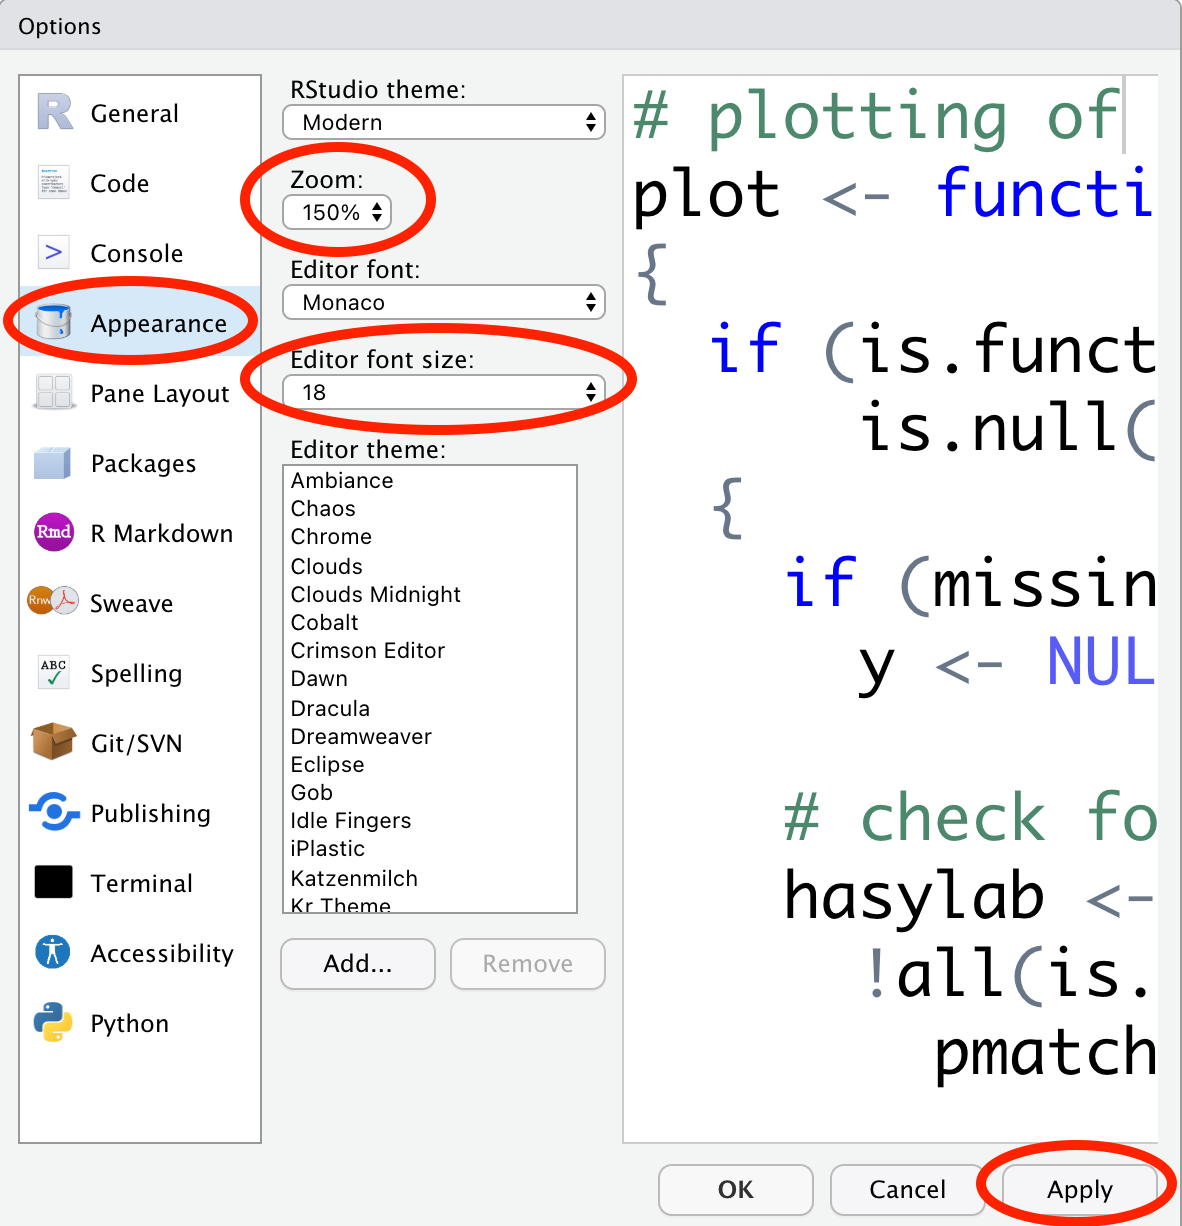
\includegraphics[width=0.5\linewidth]{pics/1size} 

}

\caption{Zoom and Editor font size}\label{fig:size}
\end{figure}

Here, we change the \emph{Zoom} to 150\% and set the \emph{Editor font size} to 18.

\textbf{\emph{b. Four panels of RStudio}}

Now, the RStudio interface is clearer with bigger font size. Although RStudio has four panels, not all of them are visible to us at the beginning (Figure \ref{fig:open}).

\begin{figure}

{\centering 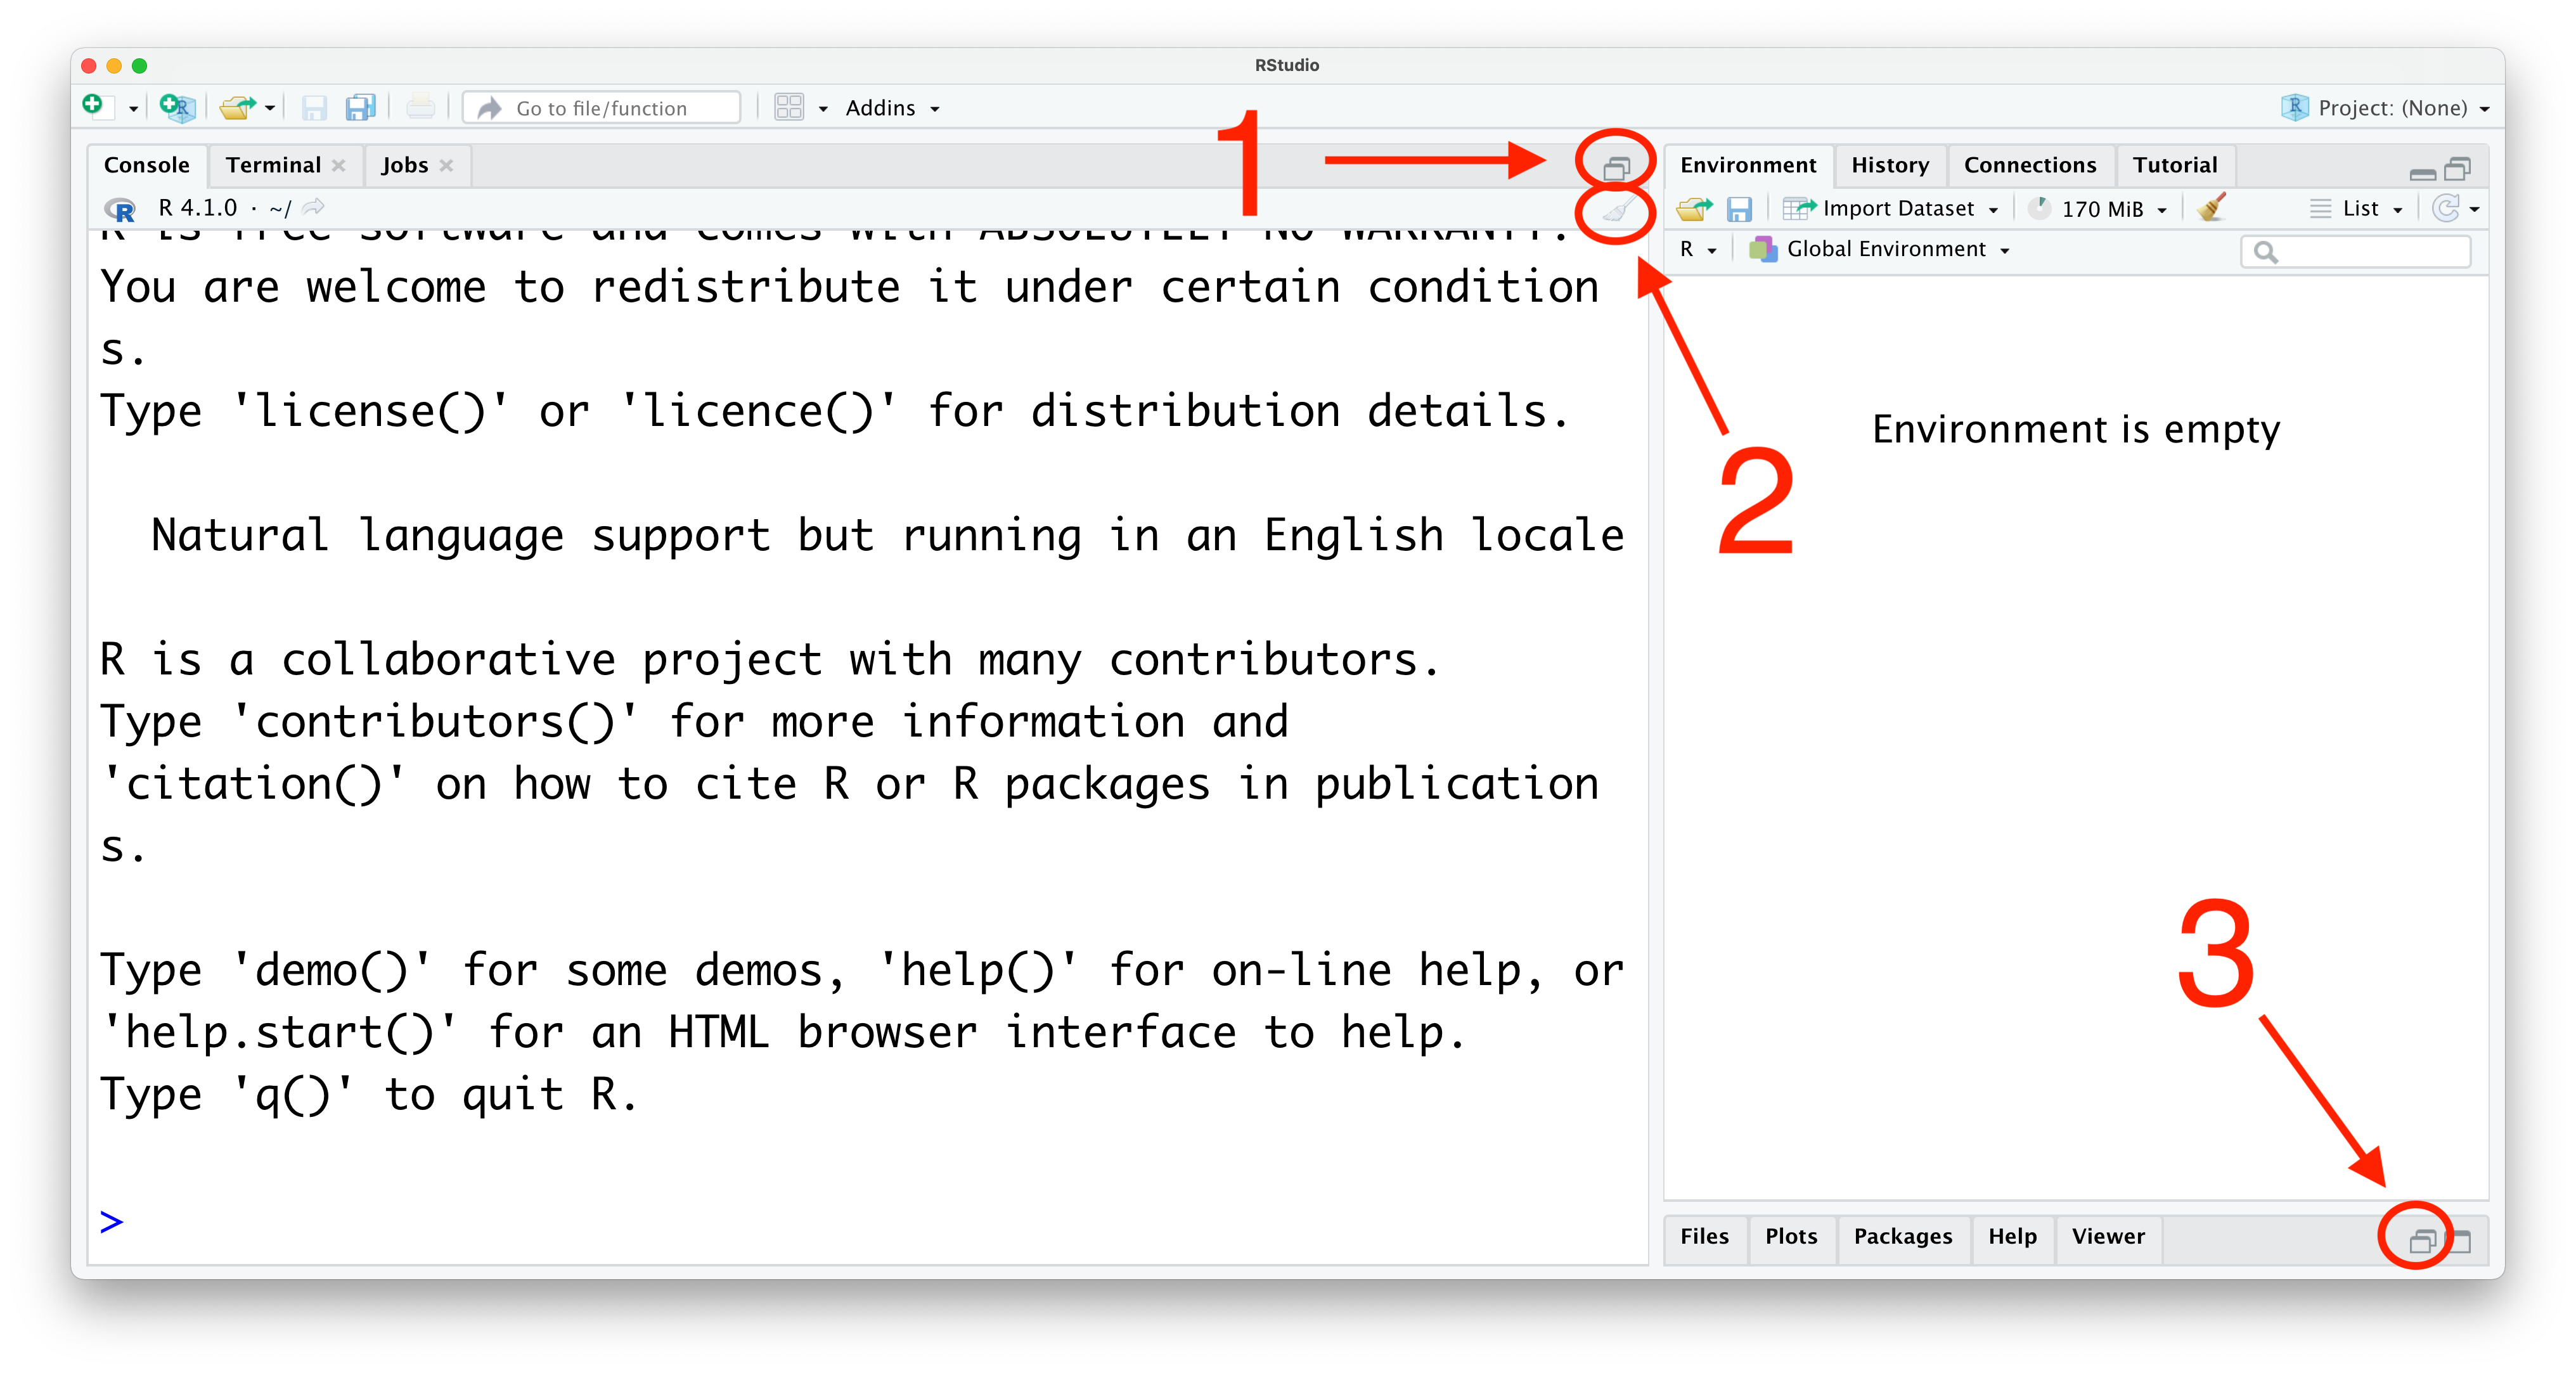
\includegraphics[width=1\linewidth]{pics/1open} 

}

\caption{Unfold panels}\label{fig:open}
\end{figure}

In Figure \ref{fig:open}, we have labeled three useful buttons as 1, 2, and 3. By clicking buttons 1 and 3, you can reveal the two hidden panels. \footnote{Note that you may see different panels hidden when you open RStudio for the first time, depending on the RStudio version. However, you can always reveal the hidden panels by clicking the corresponding buttons like Buttons 1 and 3 in Figure \ref{fig:open}.}
By clicking button 2, we can clear the content in the bottom left panel as shown in the following figure.

\begin{figure}

{\centering 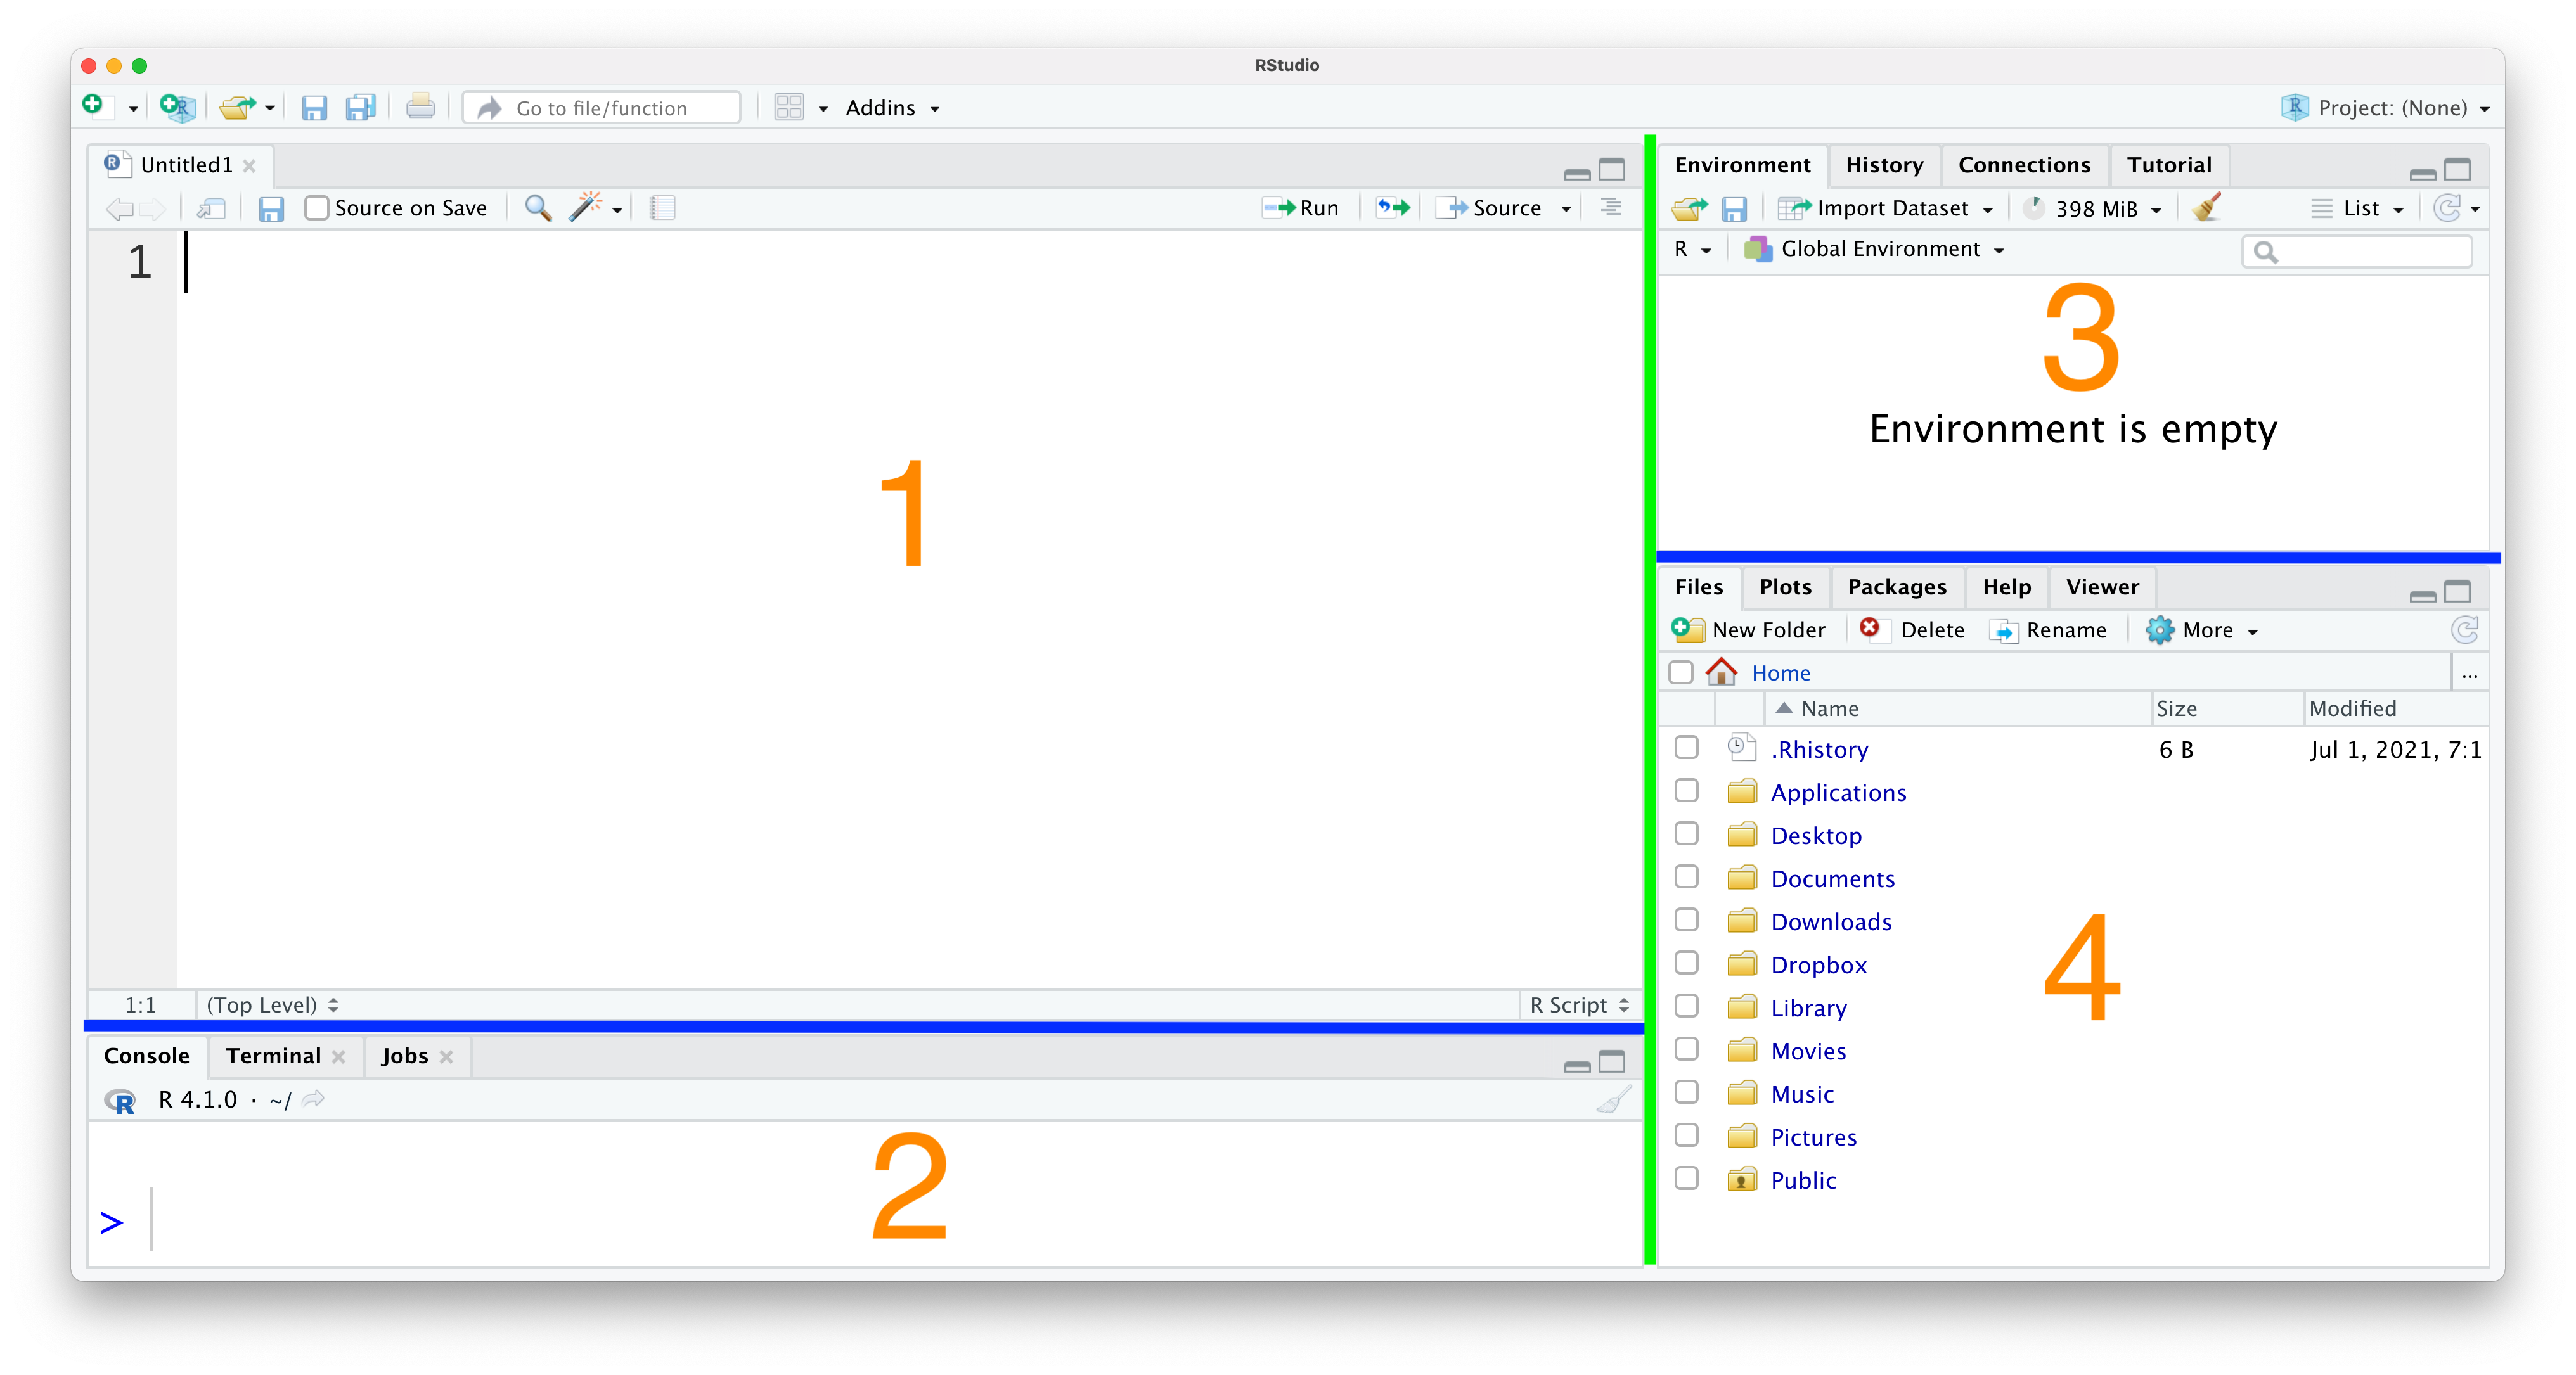
\includegraphics[width=1\linewidth]{pics/1four} 

}

\caption{Four panels}\label{fig:four}
\end{figure}

Now, let's take a close look at all four panels, which are labeled as 1-4 in Figure \ref{fig:four}. You can change the size of each panel by dragging the two blue slides up or down and the green slide left or right.

\begin{itemize}
\item
  Panels 1 and 2 are located to the left of the green line, and are collectively called the \textbf{Code Area}. We will introduce them next.
\item
  Panels 3 and 4 are located to the right of the green line, and are collectively called \textbf{R Support Area}. We will introduce these two panels in later sections. \textbf{Add the section numbers when available}
\end{itemize}

\textbf{\emph{c.~Console}}

Now, let's introduce the panel 2 in Figure \ref{fig:four}, which is usually called the \textbf{Console}.

By clicking the mouse on the line after the \texttt{\textgreater{}} symbol, you can see a blinking cursor, indicating that R is ready to accept codes. Let's type 1 + 2 and press Return (on Mac) or Enter (on Windows).

\begin{infobox}{caution}
It is a good habit to add spaces around an operator to increase readability of the code.

\end{infobox}

\begin{figure}

{\centering 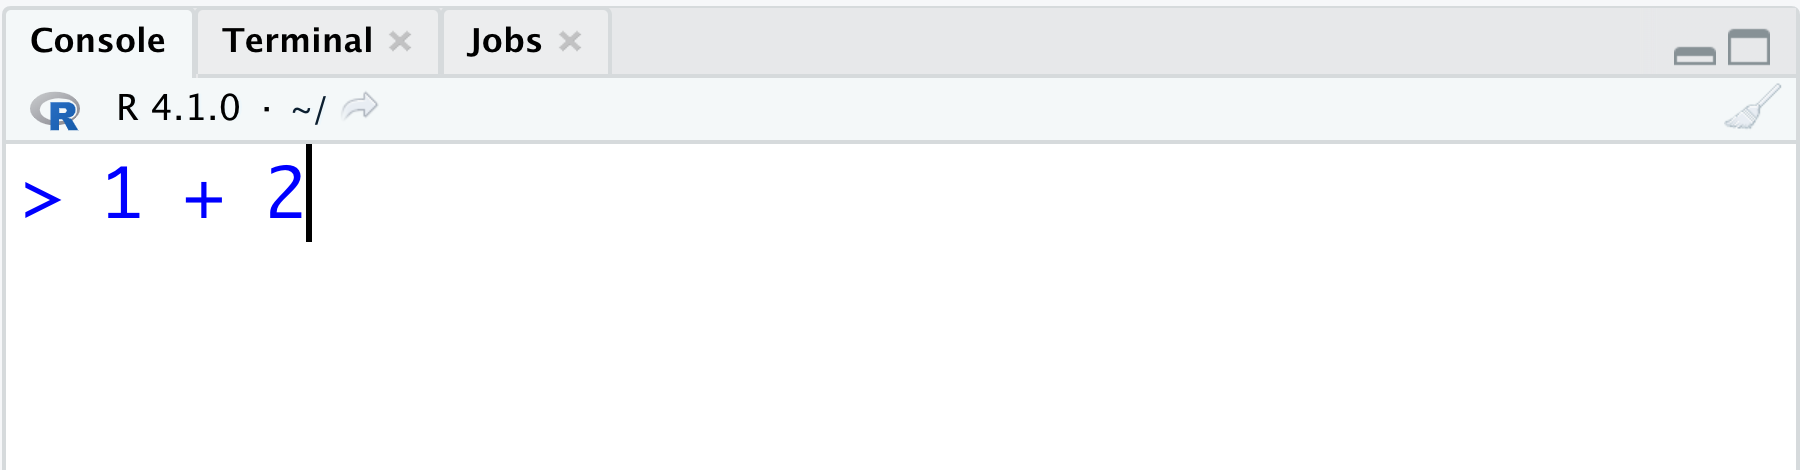
\includegraphics[width=0.7\linewidth]{pics/1code} 

}

\caption{Writing code in the console}\label{fig:code}
\end{figure}

Hooray! You have successfully ran our first piece of R code and gotten the correct answer 3. Note that the blinking cursor now appears on the next line, ready to accept a new line of code.

\begin{figure}

{\centering 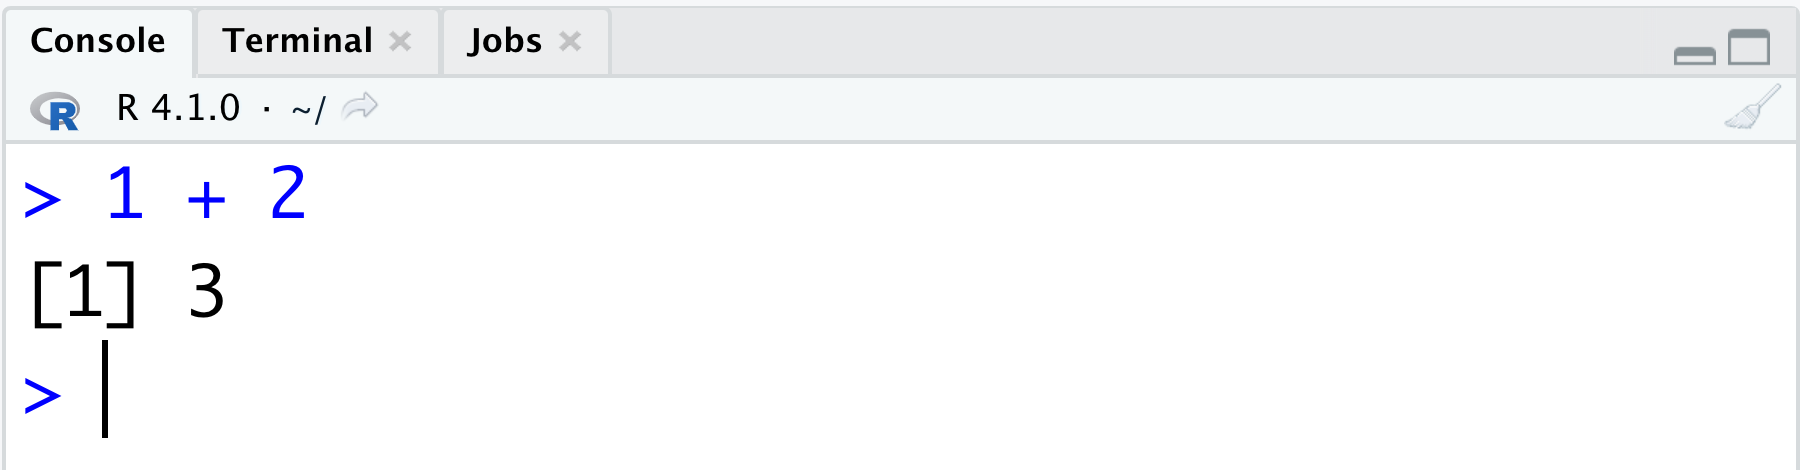
\includegraphics[width=0.7\linewidth]{pics/1answer} 

}

\caption{R code(2)}\label{fig:answer}
\end{figure}

Although the console may work well for some quick calculations, you need to resort to the panel 1 in Figure \ref{fig:four} (usually called the \textbf{Editor}) to save our work and run multiple lines of code at the same time.

\textbf{\emph{d.~Save R codes as scripts}}

The \textbf{Editor} panel is the go-to place to write complicated R codes, which you can save as R scripts for repeated use in the future.

Firstly, we will introduce how to run codes in scripts. Let's go to the editor and type 1 + 2. To run this line of code, you can click the \emph{Run} button. The keyboard shortcut of running this line of code is Cmd+Return on Mac or Ctrl+Enter on Windows.

\begin{figure}

{\centering 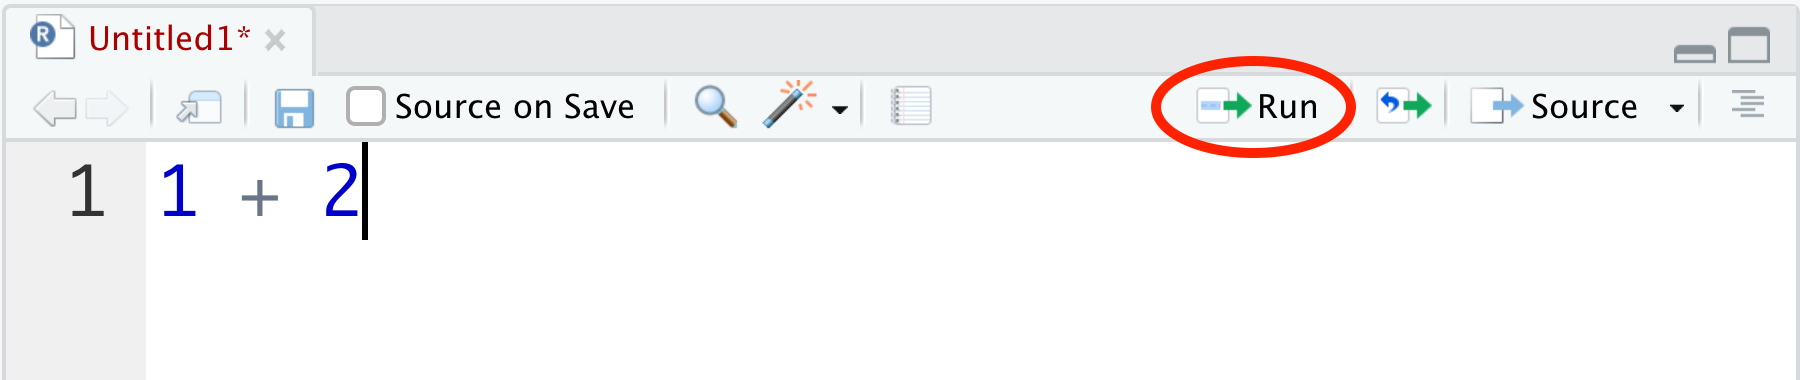
\includegraphics[width=0.7\linewidth]{pics/1run} 

}

\caption{script}\label{fig:run}
\end{figure}

RStudio will then send the line of code to the console and execute the code.

After finishing writing codes in the editor, you can save them as a script. To do that, you can click the \emph{Save} button as shown in the Figure \ref{fig:save1}. The keyboard shortcut of saving files is Cmd+S on Mac or Ctrl+S on Windows.

\begin{figure}

{\centering 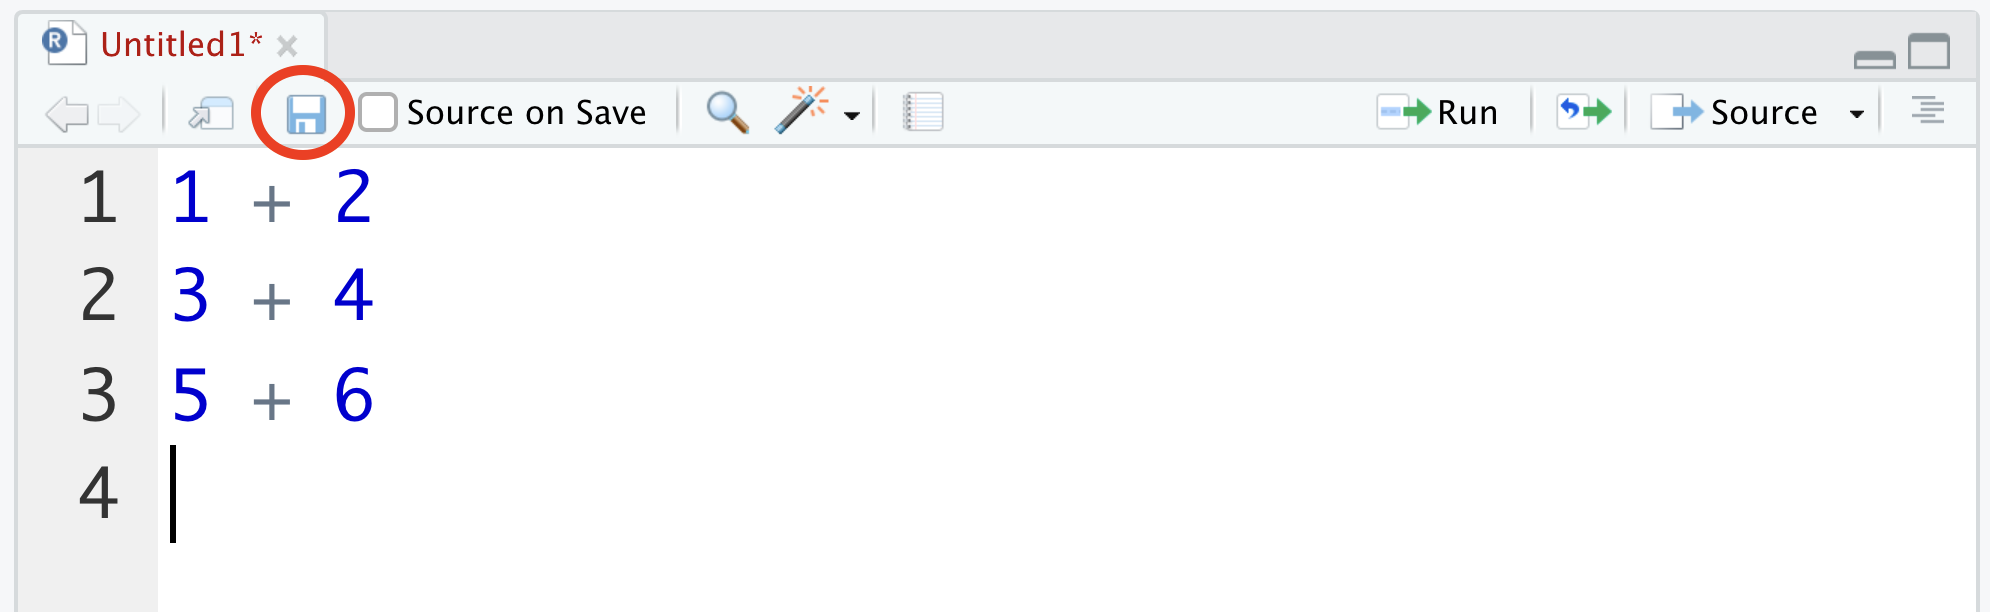
\includegraphics[width=0.7\linewidth]{pics/1save1} 

}

\caption{Save (I)}\label{fig:save1}
\end{figure}

Then you would see a pop-up file dialog box, asking you for a file name and location to save it to. Let's call it lesson1.1 here.

\begin{figure}

{\centering 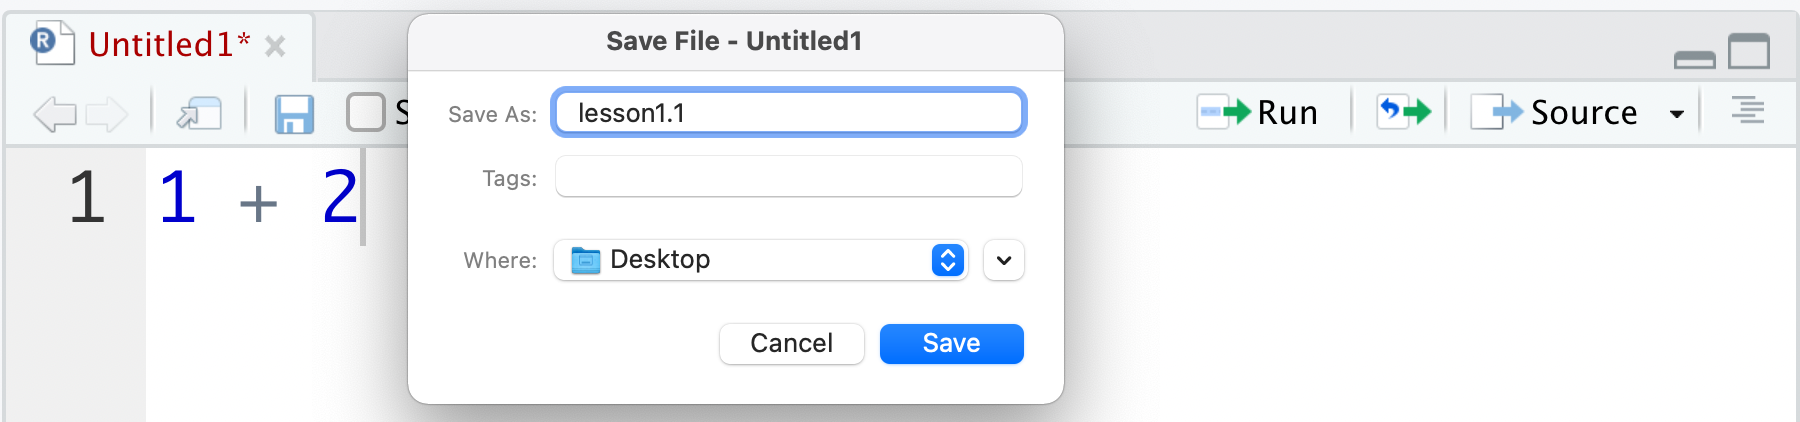
\includegraphics[width=0.7\linewidth]{pics/1save2} 

}

\caption{Save (II)}\label{fig:save2}
\end{figure}

After saving files successfully, you can confirm the name of the R script on the top.

\begin{figure}

{\centering 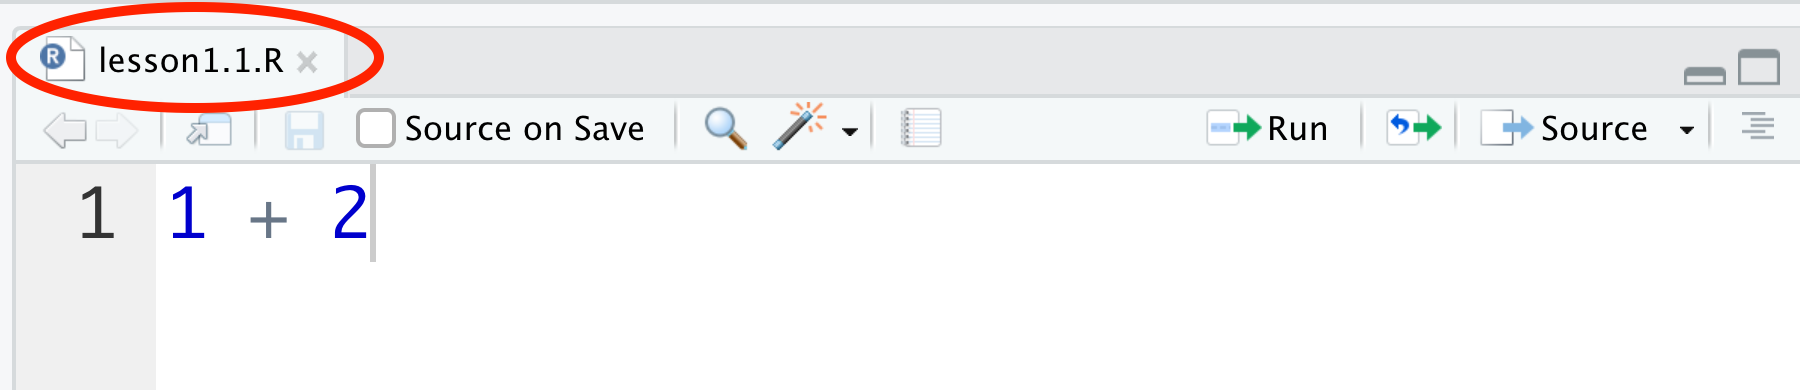
\includegraphics[width=0.7\linewidth]{pics/1save3} 

}

\caption{Save (III)}\label{fig:save3}
\end{figure}

Lastly, if you want to create a new R script, we can click the \texttt{+} button on the menu, then select \emph{R Script}. Note that there are quite a few other options including \emph{R Markdown}, which will be introduced in \textbf{Section???}. Then you will see a new file created.

\begin{figure}

{\centering 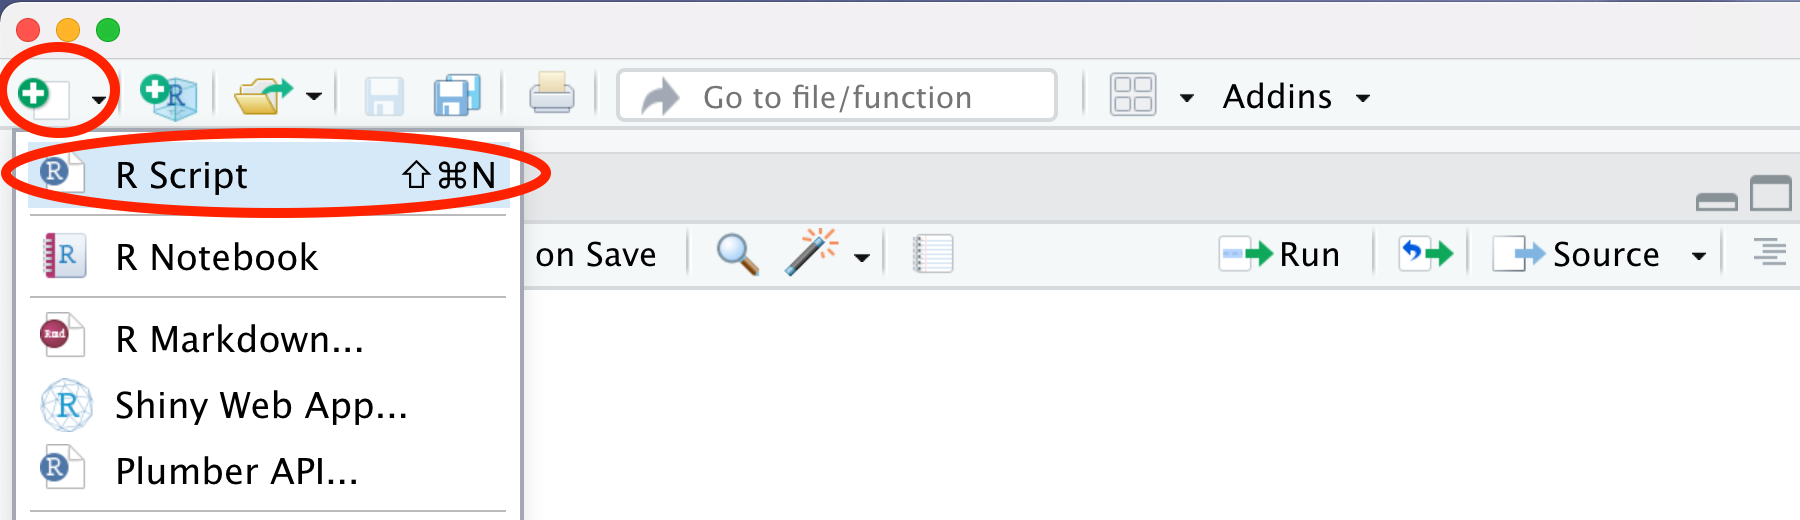
\includegraphics[width=0.7\linewidth]{pics/1new} 

}

\caption{create a new script}\label{fig:new}
\end{figure}

\hypertarget{install-and-load-r-packages}{%
\subsection{Install and load R packages}\label{install-and-load-r-packages}}

Now, you have had a basic understanding of RStudio, it is time to introduce \textbf{R packages}, which greatly extend the capabilities of base R. There are a large number of publicly available R packages. As of July 2021, there are more than 17K R packages on Comprehensive R Archive Network (CRAN), with many others located in Bioconductor, GitHub, and other repositories.

To install an R package, you need to use a built-in R \textbf{function} , which is \texttt{install.packages()}. A \textbf{function} takes in \textbf{arguments} (inputs) and performs a specific task. After the function name, we always need to put \textbf{a pair of parentheses} with the arguments inside.

While there are many built-in R functions, R packages usually contain many useful functions as well, and we can also write our own functions, which will be introduce in Section ???.

With \texttt{install.packages()}, the argument is the package name with a pair of quotation marks around it. The task it performs is installing the specific package into R. Here, you will install the companion package for this book, named \texttt{r02pro}, a.k.a. \emph{R Zero to Pro}. The \texttt{r02pro} package contains several data sets that will be used throughout the book, and interactive exercises for each subsection.

\begin{Shaded}
\begin{Highlighting}[]
\FunctionTok{install.packages}\NormalTok{(}\StringTok{"r02pro"}\NormalTok{)}
\end{Highlighting}
\end{Shaded}

\begin{infobox}{caution}
If you miss the right parenthesis, R will show a plus on the next line (as shown in Figure \ref{fig:right1}), waiting for more input to complete the command. If this happens, you can either enter the right parenthesis, or press ESC to escape this command. When you see a blinking cursor after the \texttt{\textgreater{}} symbol, you can write new codes again.

\end{infobox}

\begin{figure}

{\centering 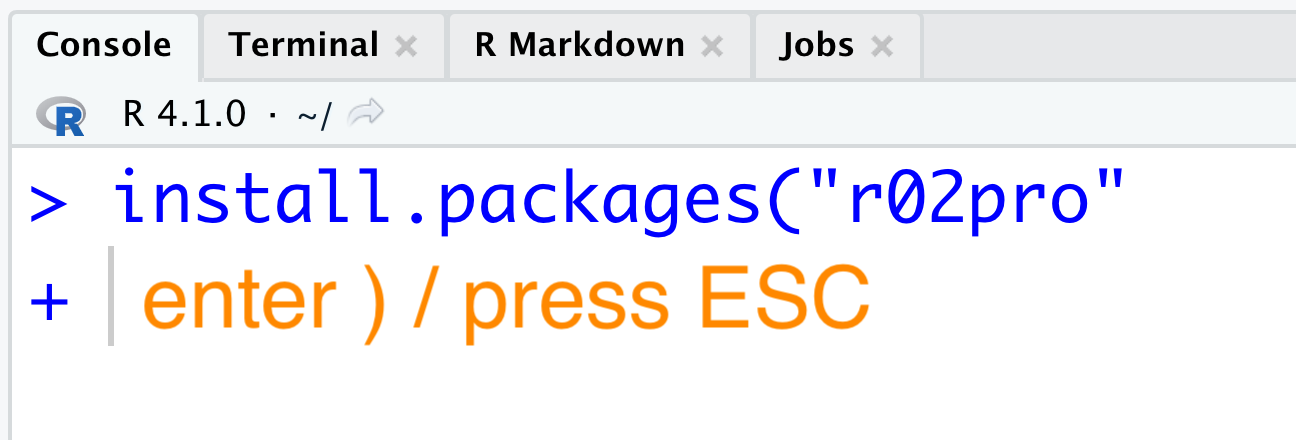
\includegraphics[width=0.7\linewidth]{pics/1right} 

}

\caption{Miss the right parenthesis}\label{fig:right1}
\end{figure}

After a package is installed, you still need to load it into R before using it. To load a package, we use the \texttt{library()} function with the package name as its argument. Here, the quotation marks are not necessary.

\begin{Shaded}
\begin{Highlighting}[]
\FunctionTok{library}\NormalTok{(r02pro)}
\end{Highlighting}
\end{Shaded}

Note that once a package is installed, you don't need to install it again on the same machine. However, when starting a new R session, you would need to load the package again.

\begin{infobox}{caution}
Quotation marks are necessary for installing R packages, but are not necessary for loading packages. If we install packages without quotation marks. We will see an error message, showing \emph{object not found}.

\end{infobox}

\begin{Shaded}
\begin{Highlighting}[]
\FunctionTok{install.packages}\NormalTok{(r02pro)}
\end{Highlighting}
\end{Shaded}

\begin{verbatim}
#> Error in endsWith(pkgs, ".tgz"): non-character object(s)
\end{verbatim}

\hypertarget{exercise-setup}{%
\subsection{Exercise setup}\label{exercise-setup}}

Having installed and loaded the \texttt{r02pro} package, let's introduce how to do the interactive exercise.
To setup the exercise, we use the \texttt{r02pro()} function with the subsection number as the argument. For example, to do the exercise for Section \ref{Installation}, we can run the following code.

\begin{Shaded}
\begin{Highlighting}[]
\FunctionTok{r02pro}\NormalTok{(}\FloatTok{1.1}\NormalTok{)}
\end{Highlighting}
\end{Shaded}

Upon running the code, a new browser window containing the interactive exercise will pop up. You can then do the exercise. The majority of the exercises ask you to write R codes to accomplish tasks. When finishing writing codes in the corresponding box, you can press the \emph{Run Code} button to run it. \textbf{Do we need to have the screenshot for this?}

\hypertarget{Calculator}{%
\section{Use R as a Fancy Calculator}\label{Calculator}}

While R is super powerful, it is, first of all, a very fancy calculator.

\hypertarget{add-comments-using}{%
\subsection{Add comments using ``\#''}\label{add-comments-using}}

The first item we will cover is about adding comments. In R, you can add comments using the pound sign \texttt{\#}. In each line, anything after \texttt{\#} are comments, which will be ignored by R. Let's see an example,

\begin{Shaded}
\begin{Highlighting}[]
\DecValTok{6} \SpecialCharTok{{-}} \DecValTok{1} \SpecialCharTok{/} \DecValTok{2} \CommentTok{\#first calculate 1/2=0.5, then 6{-}0.5=5.5}
\end{Highlighting}
\end{Shaded}

\begin{verbatim}
#> [1] 5.5
\end{verbatim}

Just looking at the resulting value 5.5, you may not know the detail of the calculation process. The comment informs you the operation order: the division is calculated before the subtraction.

In general, adding comments to codes is a very good practice, as it greatly increases readability and make collaboration easier. We will also add many comments in our codes to help you learn R.

\hypertarget{basic-calculation}{%
\subsection{Basic calculation}\label{basic-calculation}}

Now let's start to use R as a calculator! You can use R to do addition, subtraction, multiplication,division, and combine multiple basic operations. You can also calculate the square root, absolute value and the sign of a number.

\begin{tabular}{l|l}
\hline
Operation & Explanation\\
\hline
1 + 2 & addition\\
\hline
1 - 2 & subtraction\\
\hline
2 * 4 & multiplication\\
\hline
2 / 4 & division\\
\hline
6 - 1 / 2 & multiple operations\\
\hline
sqrt(100) & square root\\
\hline
abs(-3) & absolute value\\
\hline
sign(-3) & sign\\
\hline
\end{tabular}

While the first seven operations in the table look intuitive, you may be wondering, what does the \texttt{sign()} function mean here? Is it a stop sign?

\begin{center}
\includegraphics[width=0.16\linewidth]{pics/1stop} \end{center}

Sometimes, you may have no idea how a particular function works. Fortunately, R provides a detailed documentation for each function. There are three ways to ask for help in R.

\begin{itemize}
\tightlist
\item
  Use question mark followed by the function name, e.g.~\texttt{?sign}\\
\item
  Use help function, e.g.~\texttt{help(sign)}
\item
  Use the help window in RStudio, as shown in Figure \ref{fig:help}. The help window is the panel 4 of Figure \ref{fig:four} in Section \ref{Installation}. Then type in the function name in the box to the right of the magnifying glass and press return.
\end{itemize}

\begin{figure}

{\centering 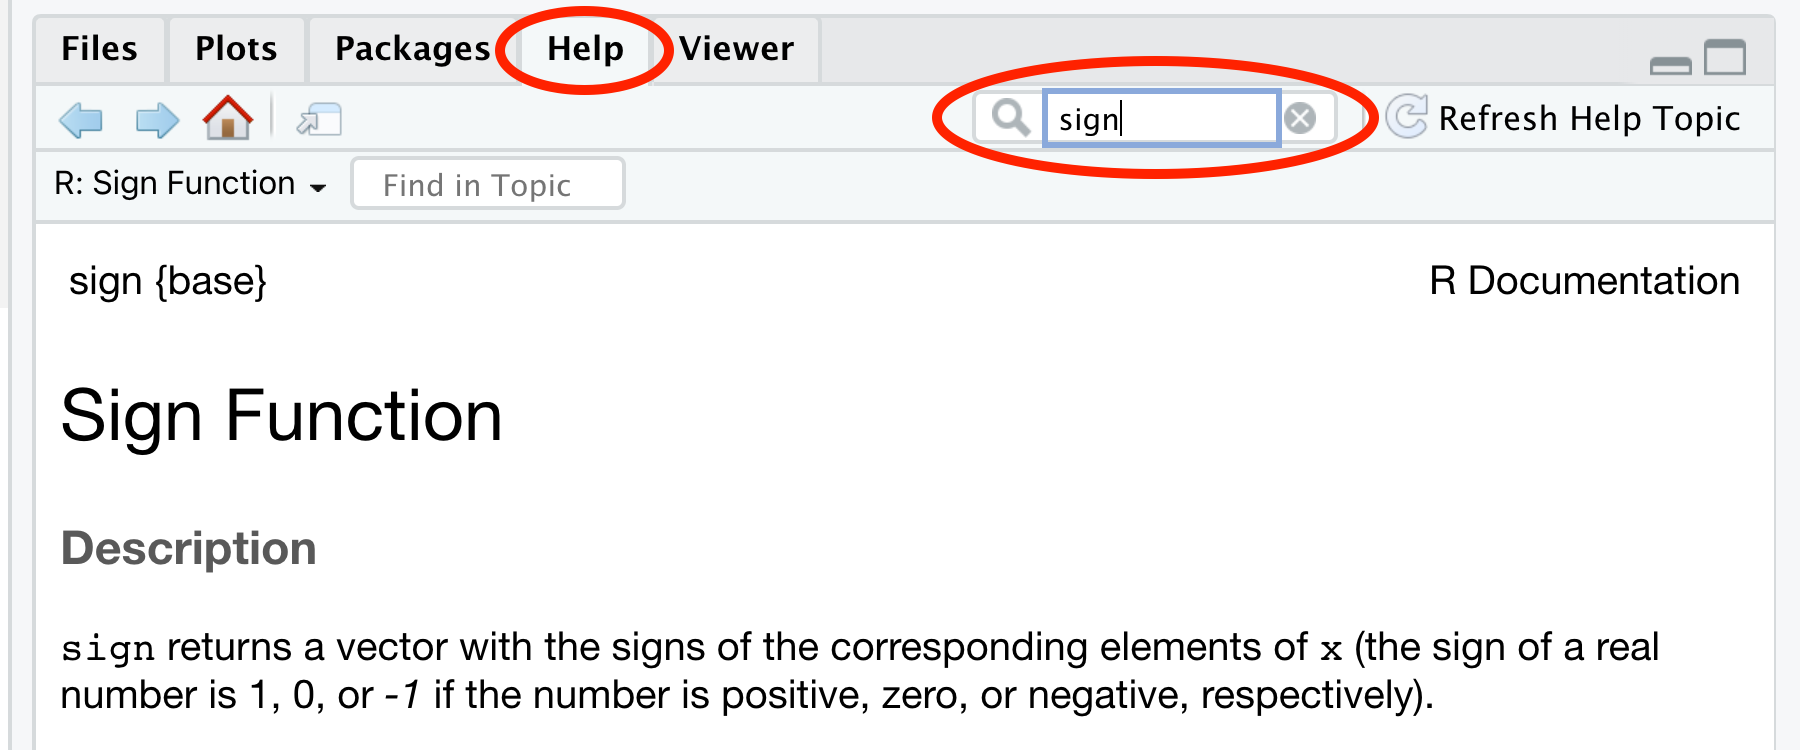
\includegraphics[width=0.7\linewidth]{pics/1help} 

}

\caption{Ask for help}\label{fig:help}
\end{figure}

\hypertarget{approximation}{%
\subsection{Approximation}\label{approximation}}

After learning about doing basic calculations, let's move on to do approximation in R. When you do division, for example, when computing \texttt{7\ /\ 3}, the answer is not a whole number since 7 is not divisible by 3. Under these circumstances, approximation operators are very handy to use. Let's take \texttt{7\ /\ 3} as the example.

\textbf{\emph{a. Get the integer part and the remainder}}

\begin{tabular}{l|l}
\hline
Code & Name\\
\hline
7\%/\%3 = 2 & integer division\\
\hline
7\%\%3 = 1 & modulus\\
\hline
\end{tabular}

We all know that 7 = 3 * \textbf{2} + \textbf{1}. So the \emph{integer division} will pick up the integer part, which is 2 here; and the \emph{modulus} will get the remainder, which is 1.

\textbf{\emph{b. Get the nearby integer}}

\begin{Shaded}
\begin{Highlighting}[]
\FunctionTok{floor}\NormalTok{(}\DecValTok{7} \SpecialCharTok{/} \DecValTok{3}\NormalTok{)   }
\FunctionTok{ceiling}\NormalTok{(}\DecValTok{7} \SpecialCharTok{/} \DecValTok{3}\NormalTok{) }
\end{Highlighting}
\end{Shaded}

Since \textbf{2} \textless= 7/3 \textless= \textbf{3}, you can use the \texttt{floor} function to find the \emph{largest integer} \textless= 7/3, which is 2; and the \texttt{ceiling} function gives the \emph{smallest integer} \textgreater= 7/3, which is 3.

\textbf{\emph{c.~Round to the nearest number}}

\begin{Shaded}
\begin{Highlighting}[]
\FunctionTok{round}\NormalTok{(}\DecValTok{7} \SpecialCharTok{/} \DecValTok{3}\NormalTok{)   }
\FunctionTok{round}\NormalTok{(}\DecValTok{7} \SpecialCharTok{/} \DecValTok{3}\NormalTok{, }\AttributeTok{digits =} \DecValTok{3}\NormalTok{)}
\end{Highlighting}
\end{Shaded}

The \texttt{round} function follows the \textbf{rounding principle}. By default, you will get the nearest integer to \texttt{7\ /\ 3}, which is \texttt{2}. If you want to control the approximation accuracy, you can add a \texttt{digits} argument to specify how many digits you want after the decimal point. Here you will get \texttt{2.333} after adding \texttt{digits\ =\ 3}.

\hypertarget{power-logarithm}{%
\subsection{Power \& logarithm}\label{power-logarithm}}

You can also use R to do \emph{power} and \emph{logarithmic} operations.

Generally, you can use \textbf{\^{}} to do power operations. For example, \texttt{10\^{}5} will give us 10 to the power of 5. Here, 10 is the \emph{base} value, and 5 is the \emph{exponent}. The result is 100000, but it is shown as \texttt{1e+05} in R. That's because R uses the so-called \emph{scientific notation}.

\begin{infobox}{caution}
\textbf{scientific notation}: a common way to express numbers which are too large or too small to be conveniently written in decimal form. Generally, it expresses numbers in forms of \(m \times 10^n\) and R uses the \textbf{e notation}. Note that the \textbf{e notation} has nothing to do with the natural number \(e\). Let's see some examples,
\begin{align}
1 \times 10^5 &= \mbox{1e+05}\\
2 \times 10^4 &= \mbox{2e+04}\\
1.2 \times 10^{-3} &= \mbox{1.2e-03}
\end{align}

\end{infobox}

In mathematics, the \emph{logarithmic operations} are inverse to the power operations. If \textbf{\(b^y = x\)} and you only know \emph{\(b\)} and \emph{\(x\)}, you can do logarithm operations to solve \emph{\(y\)} using the general form \textbf{\(y = \log(x, b)\)}, which is called the logarithm of \(x\) with base \(b\).

In R, logarithm functions with base value of 10, 2, or the natural number \(e\) have shortcuts \texttt{log10()}, \texttt{log2()}, and \texttt{log()}, respectively. Let's see an example of \texttt{log10()}, the logarithm function with base \emph{10}.

\begin{Shaded}
\begin{Highlighting}[]
\DecValTok{10}\SpecialCharTok{\^{}}\DecValTok{6} 
\FunctionTok{log10}\NormalTok{(}\FloatTok{1e6}\NormalTok{) }\CommentTok{\#log10() = log(x, 10)}
\end{Highlighting}
\end{Shaded}

Next, let's see \texttt{log2()}, the logarithm function with base \emph{2}.

\begin{Shaded}
\begin{Highlighting}[]
\DecValTok{2}\SpecialCharTok{\^{}}\DecValTok{10}
\FunctionTok{log2}\NormalTok{(}\DecValTok{1024}\NormalTok{)  }\CommentTok{\#log2() = log(x, 2)}
\end{Highlighting}
\end{Shaded}

Before moving on to the natural logarithm, note that the natural number \(e\) needs to be written as \texttt{exp(1)} in R. When you want to do power operations on \(e\), you can simply change the argument in the function \texttt{exp()}, for example, \texttt{exp(3)} is \(e\) to the power of 3. Here, \texttt{log()} without specifying the \texttt{base} argument represents the logarithm function with base \(e\).

\begin{Shaded}
\begin{Highlighting}[]
\FunctionTok{exp}\NormalTok{(}\DecValTok{1}\NormalTok{)      }
\FunctionTok{exp}\NormalTok{(}\DecValTok{3}\NormalTok{)}
\FunctionTok{log}\NormalTok{(}\FunctionTok{exp}\NormalTok{(}\DecValTok{3}\NormalTok{))  }\CommentTok{\#log() = log(x, exp(1))}
\end{Highlighting}
\end{Shaded}

\hypertarget{trigonometric-function}{%
\subsection{Trigonometric function}\label{trigonometric-function}}

R also provides the common trigonometric functions.

\begin{Shaded}
\begin{Highlighting}[]
\FunctionTok{cos}\NormalTok{(pi)}
\FunctionTok{acos}\NormalTok{(}\SpecialCharTok{{-}}\DecValTok{1}\NormalTok{)}
\end{Highlighting}
\end{Shaded}

Here, \texttt{acos()} is the inverse function of \texttt{cos()}. If we set \(cos(a) = b\), then we will get \(acos(b) = a\).

\begin{Shaded}
\begin{Highlighting}[]
\FunctionTok{sin}\NormalTok{(pi}\SpecialCharTok{/}\DecValTok{2}\NormalTok{)}
\FunctionTok{asin}\NormalTok{(}\DecValTok{1}\NormalTok{)}
\end{Highlighting}
\end{Shaded}

Similarly, \texttt{asin()} is the inverse function of \texttt{sin()}. If we set \(sin(a) = b\), then we will get \(asin(b) = a\).

\begin{Shaded}
\begin{Highlighting}[]
\FunctionTok{tan}\NormalTok{(pi}\SpecialCharTok{/}\DecValTok{4}\NormalTok{)}
\FunctionTok{atan}\NormalTok{(}\DecValTok{1}\NormalTok{)}
\end{Highlighting}
\end{Shaded}

Also, \texttt{atan()} is the inverse function of \texttt{tan()}. If we set \(tan(a) = b\), then we will get \(atan(b) = a\).

\hypertarget{exercise}{%
\subsection{Exercise}\label{exercise}}

You can run the following code to do the exercise.

\begin{Shaded}
\begin{Highlighting}[]
\FunctionTok{r02pro}\NormalTok{(}\FloatTok{1.2}\NormalTok{)}
\end{Highlighting}
\end{Shaded}

\hypertarget{r-objects}{%
\chapter{R Objects}\label{r-objects}}

In R, \textbf{everything is an object}. An object can contain values of different types including numbers, characters, and any intermediate results from operations. For example, \texttt{5} is an object with the value 5.

In the last chapter, we have seen the power of R as a fancy calculator. However, in order to do more complicated and interesting tasks, we may need to store intermediate results for future use.

Let's take a look at a concrete example. Say if you want to do the following calculations involving \texttt{exp(3)\ /\ log(20,3)\ *\ 7}.

\begin{Shaded}
\begin{Highlighting}[]
\NormalTok{(}\FunctionTok{exp}\NormalTok{(}\DecValTok{3}\NormalTok{) }\SpecialCharTok{/} \FunctionTok{log}\NormalTok{(}\DecValTok{20}\NormalTok{,}\DecValTok{3}\NormalTok{) }\SpecialCharTok{*} \DecValTok{7}\NormalTok{) }\SpecialCharTok{+} \DecValTok{3} \CommentTok{\#addition}
\NormalTok{(}\FunctionTok{exp}\NormalTok{(}\DecValTok{3}\NormalTok{) }\SpecialCharTok{/} \FunctionTok{log}\NormalTok{(}\DecValTok{20}\NormalTok{,}\DecValTok{3}\NormalTok{) }\SpecialCharTok{*} \DecValTok{7}\NormalTok{) }\SpecialCharTok{{-}} \DecValTok{3} \CommentTok{\#subtraction}
\NormalTok{(}\FunctionTok{exp}\NormalTok{(}\DecValTok{3}\NormalTok{) }\SpecialCharTok{/} \FunctionTok{log}\NormalTok{(}\DecValTok{20}\NormalTok{,}\DecValTok{3}\NormalTok{) }\SpecialCharTok{*} \DecValTok{7}\NormalTok{) }\SpecialCharTok{/} \DecValTok{3} \CommentTok{\#division}
\end{Highlighting}
\end{Shaded}

You need to type the expression three times, which is a bit cumbersome. In this chapter, we will introduce how to assign the value of the object \texttt{exp(3)\ /\ log(20,3)\ *\ 7} to a name for future use. Then, for any operation involving \texttt{exp(3)\ /\ log(20,3)\ *\ 7}, you can just use the corresponding object name instead.

In R, there are a few different object types, which we will cover each of them in detail in this Chapter.

\hypertarget{Object-Assignment}{%
\section{Object Assignment}\label{Object-Assignment}}

\hypertarget{assignment-operation-with--}{%
\subsection{\texorpdfstring{Assignment Operation with \texttt{\textless{}-}}{Assignment Operation with \textless-}}\label{assignment-operation-with--}}

Firstly, we will introduce how to assign value(s) (of objects) to a name via the \emph{assignment operator}. Let's start with a simple example,

\begin{Shaded}
\begin{Highlighting}[]
\NormalTok{x\_numeric }\OtherTok{\textless{}{-}} \DecValTok{5}
\end{Highlighting}
\end{Shaded}

The assignment operation has three components.

\begin{itemize}
\tightlist
\item
  From left to right,the first component \texttt{x\_numeric} is the \textbf{object name}, which has certain naming rules which we will discuss shortly in Section \ref{Naming}.
\item
  The second component is the \textbf{assignment operator} \texttt{\textless{}-}, which is a combination of the less than sign \texttt{\textless{}} immediately followed by the minus sign \texttt{-}.
\item
  The final component is the \textbf{value} to be assigned to the name, which is 5 here.
\end{itemize}

\begin{infobox}{caution}
There is no space between \texttt{\textless{}} and \texttt{-} in the assignment operator \texttt{\textless{}-}. Note that although \texttt{=} may also appear to be working as the assignment operator, it is not recommended as \texttt{=} is usually reserved for specifying the value of arguments in a function call, which will be introduced in Section \ref{vector-patterns}.

\end{infobox}

After running the code above, you will see no output in the console, unlike the case when we ran \texttt{1\ +\ 2} which gives us the answer 3 (as shown in the Figure \ref{fig:noa}). You may be wondering, did we successfully make our first assignment operation?

\begin{figure}

{\centering 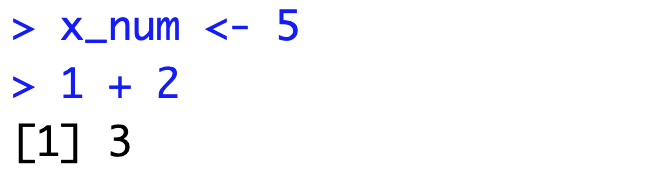
\includegraphics[width=0.7\linewidth]{pics/2noa} 

}

\caption{No output}\label{fig:noa}
\end{figure}

To verify it, you can run the code with just the object name to check its value.

\begin{Shaded}
\begin{Highlighting}[]
\NormalTok{x\_numeric}
\end{Highlighting}
\end{Shaded}

\begin{verbatim}
#> [1] 5
\end{verbatim}

Great! You get the value 5, indicating that you have successfully assigned the value 5 to \texttt{x\_numeric}.

In addition to assigning the value to a name, you can also assign the value of any R expression to it. In this case, R will first calculate the value of the expression and assign the value to the name. Let's see the following example.

\begin{Shaded}
\begin{Highlighting}[]
\NormalTok{y\_numeric }\OtherTok{\textless{}{-}} \FunctionTok{exp}\NormalTok{(}\DecValTok{3}\NormalTok{) }\SpecialCharTok{/} \FunctionTok{log}\NormalTok{(}\DecValTok{20}\NormalTok{,}\DecValTok{3}\NormalTok{) }\SpecialCharTok{*} \DecValTok{7}
\NormalTok{y\_numeric}
\end{Highlighting}
\end{Shaded}

\begin{verbatim}
#> [1] 51.56119
\end{verbatim}

Using the object name \texttt{y\_numeric}, you can do the same three calculations introduced at the beginning of this chapter as follows.

\begin{Shaded}
\begin{Highlighting}[]
\NormalTok{y\_numeric }\SpecialCharTok{+} \DecValTok{3}
\NormalTok{y\_numeric }\SpecialCharTok{{-}} \DecValTok{3}
\NormalTok{y\_numeric }\SpecialCharTok{/} \DecValTok{3}
\end{Highlighting}
\end{Shaded}

Clearly, using the object name, we greatly simplify our code and avoid the redundancy.

Note that R object names are \textbf{case-sensitive}. For example, you have defined \texttt{x\_numeric}, but if you type \texttt{X\_numeric}, you will get an error message as follow.

\begin{Shaded}
\begin{Highlighting}[]
\NormalTok{X\_numeric}
\end{Highlighting}
\end{Shaded}

\begin{verbatim}
#> Error in eval(expr, envir, enclos): object 'X_numeric' not found
\end{verbatim}

\hypertarget{review-objects-in-environment}{%
\subsection{Review objects in environment}\label{review-objects-in-environment}}

After creating the objects \texttt{x\_numeric} and \texttt{y\_numeric}, they also appear in the \textbf{Environment}, located in the top right \ref{fig:quo} panel (\textbf{panel3 in Figure \ref{fig:four}}). You can check all the named objects and their values in this area. It is helpful to monitor the environment from time to time to make sure everything looks fine.

You can also see the list of all the objects you have defined using function \texttt{ls()}.

\begin{Shaded}
\begin{Highlighting}[]
\FunctionTok{ls}\NormalTok{()}
\end{Highlighting}
\end{Shaded}

\begin{verbatim}
#>  [1] "Code"        "d"           "Explanation" "name"        "Name"       
#>  [6] "norm_dat"    "norm_dat_1"  "norm_dat_2"  "norm_dat_3"  "Operation"  
#> [11] "Pattern"     "Section"     "x"           "x_numeric"   "y_numeric"
\end{verbatim}

\hypertarget{Naming}{%
\subsection{Object naming rule}\label{Naming}}

Now you have created two objects named \texttt{x\_numeric} and \texttt{y\_numeric}. In general, R is very flexible in the name you give to an object,however, there are three important rules you need to follow.

\textbf{\emph{a. Must start with a letter or . (period)}}\\
If starting with period, the second character can't be a number.

\textbf{\emph{b. Can only contain letters, numbers, \texttt{\_} (underscore), and \texttt{.} (period)}}
One recommended naming style is to only use lower case letters and numbers, and use underscore to separate words within a name. So you can use relatively longer names that is more readable.

\textbf{\emph{c.~Can not use special keywords as names.}}
For example, \texttt{TRUE\ \textless{}-\ 12} is not permitted as \texttt{TRUE} is a special keyword in R. You can see from the following that this assignment operation leads to an error message.

\begin{Shaded}
\begin{Highlighting}[]
\ConstantTok{TRUE} \OtherTok{\textless{}{-}} \DecValTok{12}
\end{Highlighting}
\end{Shaded}

\begin{verbatim}
#> Error in TRUE <- 12: invalid (do_set) left-hand side to assignment
\end{verbatim}

Some commonly used keywords that cannot be used as names are listed as below.

\begin{tabular}{l|l}
\hline
break & NA\\
\hline
else & NaN\\
\hline
FALSE & next\\
\hline
for & repeat\\
\hline
function & return\\
\hline
if & TRUE\\
\hline
Inf & while\\
\hline
\end{tabular}

\hypertarget{object-types}{%
\subsection{Object types}\label{object-types}}

In this section, you have learned about how to assign a value to a name. The objects we used are of \emph{numeric} type. In addition, an object may contain more than one values. Also it can also be of other types than \emph{numeric}, including \emph{character}, \emph{logical} and the combination of different types. Depending on the structure, the object belongs to one particular type. We will give a comprehensive treatment to the following object types in this chapter.

\begin{tabular}{l|l}
\hline
Type & Section\\
\hline
Vector & \textbackslash{}@ref(vector)\\
\hline
Matrix & \textbackslash{}@ref(matrix)\\
\hline
Array & \textbackslash{}@ref(array)\\
\hline
Data Frame & \textbackslash{}@ref(dataframe)\\
\hline
List & \textbackslash{}@ref(list)\\
\hline
\end{tabular}

While some of the object types look more intuitive than others, you have nothing to worry about since we have this whole chapter devoted to the details of R objects. Objects are the building blocks of R programming and it will be time well spent mastering every object type.

\hypertarget{exercise-1}{%
\subsection{Exercise}\label{exercise-1}}

You can run the following code to do the exercise.

\begin{Shaded}
\begin{Highlighting}[]
\FunctionTok{r02pro}\NormalTok{(}\FloatTok{2.1}\NormalTok{)}
\end{Highlighting}
\end{Shaded}

\hypertarget{vector}{%
\section{Numeric Vector, Character Vector, \& Logical Vector}\label{vector}}

In the last section, you have had a basic understanding of R objects and how to do object assignments. From this section, we will start to introduce different types of R objects one by one. The first R object we want to introduce is called \textbf{vector}. \textbf{Vector} is the simplest object type in R, which contains one or more values of the \textbf{same type}. We will introduce numeric vector, character vector, and logical vector in this section. Let's begin with numeric vector.

\hypertarget{numeric-vector}{%
\subsection{Numeric vector}\label{numeric-vector}}

\textbf{\emph{a. Create numeric vectors}}

A \textbf{numeric vector} is a type of vector that only contains \emph{numbers}. For example, \texttt{6} is a numeric vector with length 1. After assigning 6 to the name \texttt{x1}, you can refer to \texttt{x1} in the following calculations.

\begin{Shaded}
\begin{Highlighting}[]
\DecValTok{6}                         \CommentTok{\#a vector with length 1}
\NormalTok{x1 }\OtherTok{\textless{}{-}} \DecValTok{6}                   \CommentTok{\#x1 is a named vector with length 1}
\NormalTok{x1                        }\CommentTok{\#check the value of x1}
\end{Highlighting}
\end{Shaded}

But can a numeric vector contain more than one numbers? The answer is a big YES! In R, you can use the \texttt{c()} function (\texttt{c} is short for combine) to combine values into a vector.

\begin{Shaded}
\begin{Highlighting}[]
\FunctionTok{c}\NormalTok{(}\DecValTok{1}\NormalTok{, }\DecValTok{3}\NormalTok{, }\DecValTok{3}\NormalTok{, }\DecValTok{5}\NormalTok{, }\DecValTok{5}\NormalTok{)          }\CommentTok{\#use c() to combine values into a vector with length 5}
\NormalTok{y1 }\OtherTok{\textless{}{-}} \FunctionTok{c}\NormalTok{(}\DecValTok{1}\NormalTok{, }\DecValTok{3}\NormalTok{, }\DecValTok{3}\NormalTok{, }\DecValTok{5}\NormalTok{, }\DecValTok{5}\NormalTok{)    }\CommentTok{\#y1 is a named vector with length 5}
\NormalTok{y1                        }\CommentTok{\#check the value of y1}
\FunctionTok{length}\NormalTok{(y1)                }\CommentTok{\#length of a vector}
\end{Highlighting}
\end{Shaded}

In this example, you have created a length-5 vector using the \texttt{c()} function with arguments containing the five numbers separated by comma. You can also assign the values to the name \texttt{y1}. You can verify the contents of \texttt{y1} and check the length of it through the \texttt{length()} function.

\textbf{If you write several numeric vectors in \texttt{c()}, you will also create a numeric vector with more than one numbers. For example, you can create a numeric vector with values from two numeric vectors.}

\begin{Shaded}
\begin{Highlighting}[]
\FunctionTok{c}\NormalTok{(}\FunctionTok{c}\NormalTok{(}\DecValTok{1}\NormalTok{,}\DecValTok{2}\NormalTok{), }\FunctionTok{c}\NormalTok{(}\DecValTok{3}\NormalTok{,}\DecValTok{4}\NormalTok{))          }\CommentTok{\#use c() to combine several numeric vectors into a numeric vector}
\NormalTok{z1 }\OtherTok{\textless{}{-}} \FunctionTok{c}\NormalTok{(}\FunctionTok{c}\NormalTok{(}\DecValTok{1}\NormalTok{,}\DecValTok{2}\NormalTok{), }\FunctionTok{c}\NormalTok{(}\DecValTok{3}\NormalTok{,}\DecValTok{4}\NormalTok{))}
\NormalTok{z1}
\FunctionTok{length}\NormalTok{(z1)}
\end{Highlighting}
\end{Shaded}

\textbf{After creating numeric vectors, you can use the function \texttt{class()} to check its }type\textbf{,}

\begin{Shaded}
\begin{Highlighting}[]
\FunctionTok{class}\NormalTok{(x1)}
\FunctionTok{class}\NormalTok{(y1) }
\FunctionTok{class}\NormalTok{(z1)}
\end{Highlighting}
\end{Shaded}

From the results, you will know that \texttt{x1}, \texttt{y1} and \texttt{z1} are both of numeric type, which is the reason why they are called \emph{numeric vectors}.

\textbf{\emph{b. Operations between two vectors}}

Since numeric vectors are made of numbers, you can do \textbf{arithmetic operations} between them, just like the fancy calculator in Section \ref{Calculator}. If two vectors are of the \textbf{same length}, the calculation is done elementwisely. In other words, R will perform the operation separately for each element. First, let's create another vector of length 1 and do addition with \texttt{x1}.

\begin{Shaded}
\begin{Highlighting}[]
\NormalTok{x2 }\OtherTok{\textless{}{-}} \DecValTok{3}
\NormalTok{x1 }\SpecialCharTok{+}\NormalTok{ x2}
\end{Highlighting}
\end{Shaded}

\begin{verbatim}
#> [1] 9
\end{verbatim}

Then obviously you will get 9!

Similarly, you can create another vector \texttt{y2} of the same length as vector \texttt{y1}. Then, you can do operations between \texttt{y1} and \texttt{y2}.

\begin{Shaded}
\begin{Highlighting}[]
\NormalTok{y2 }\OtherTok{\textless{}{-}} \FunctionTok{c}\NormalTok{(}\DecValTok{2}\NormalTok{, }\DecValTok{4}\NormalTok{, }\DecValTok{1}\NormalTok{, }\DecValTok{3}\NormalTok{, }\DecValTok{2}\NormalTok{)}
\NormalTok{y1 }\SpecialCharTok{+}\NormalTok{ y2}
\end{Highlighting}
\end{Shaded}

\begin{verbatim}
#> [1] 3 7 4 8 7
\end{verbatim}

The result is yet another length-5 vector. To check the calculation was indeed done elementwisely, you can verify that the first element is \(1 + 2 = 3\), and the second element is \(3 + 4 = 7\), etc.

Since the calculation is done elementwisely, we normally would want the two vectors to have the \emph{same length}. However, there is a \textbf{recycling} rule in R, which is sometimes quite useful and enables us to write simpler code. Specifically, if one vector is shorter than the other vector, R will \emph{recycle} (repeat) the shorter vector until it matches in length with the longer one. This recycling is particularly helpful for an operator between a length\textgreater1 vector and a length-1 vector. Let's see an example.

\begin{Shaded}
\begin{Highlighting}[]
\NormalTok{y1 }\SpecialCharTok{+}\NormalTok{ x1}
\end{Highlighting}
\end{Shaded}

\begin{verbatim}
#> [1]  7  9  9 11 11
\end{verbatim}

From the result, you can see that each element in \texttt{y1} is added by 6. The following are a few additional examples you can try.

\begin{Shaded}
\begin{Highlighting}[]
\NormalTok{y1 }\SpecialCharTok{*}\NormalTok{ x2}
\NormalTok{y1 }\SpecialCharTok{/} \DecValTok{5}
\NormalTok{y2 }\SpecialCharTok{{-}}\NormalTok{ x1}
\end{Highlighting}
\end{Shaded}

\hypertarget{character-vector-characterletter}{%
\subsection{Character vector character/letter}\label{character-vector-characterletter}}

\textbf{\emph{a. Create character vectors}}

Now, let's move to character vectors. In a \textbf{character vector}, each value is a \textbf{string}. A \textbf{string} is a sequence of characters (letters, numbers, or symbols) surrounded by a pair of double quotes (\texttt{""}) or single quotes (\texttt{\textquotesingle{}\textquotesingle{}}). To be consistent, we will stick with double quotes in this book. Let's first create a character vector with just one string. You can then check the value of this vector by typing its name and verify the vector type by using \texttt{class()}.

\begin{Shaded}
\begin{Highlighting}[]
\NormalTok{sheepstudio }\OtherTok{\textless{}{-}} \StringTok{"sheep@007"} 
\NormalTok{sheepstudio}
\FunctionTok{class}\NormalTok{(sheepstudio)}
\end{Highlighting}
\end{Shaded}

\begin{infobox}{caution}
Double quotes need to be paired in strings. If you miss the right double quote, R will show a plus on the next line, waiting for you to finish the command. If this happens, you can either enter the matching double quote, or press ESC to escape this command.

\end{infobox}

\begin{figure}

{\centering 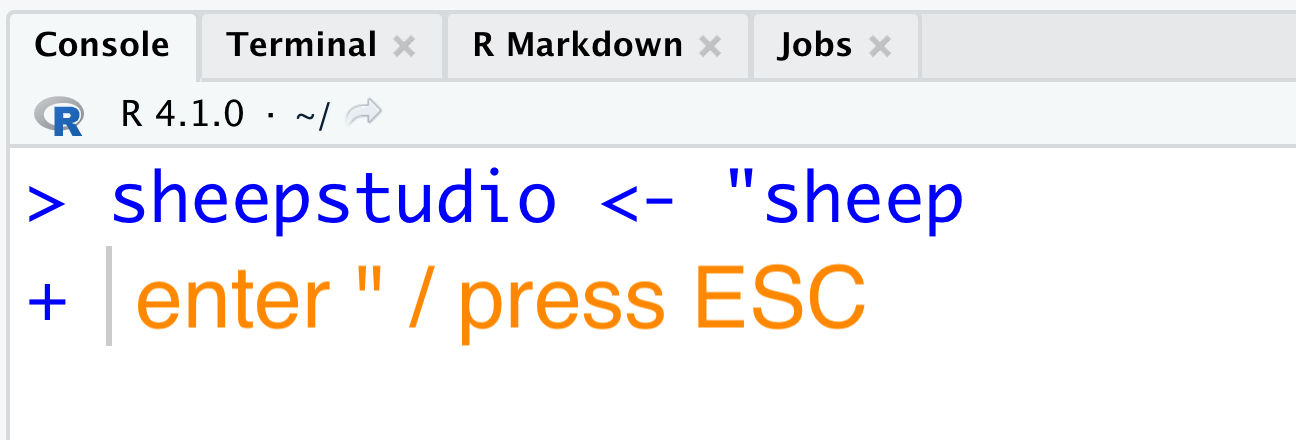
\includegraphics[width=0.7\linewidth]{pics/2quo} 

}

\caption{Miss the right quotation mark}\label{fig:quo}
\end{figure}

Similar to a numeric vector, you can use the \texttt{c()} function to combine several strings to create a character vector. You can verify the number of strings in the character vector by using \texttt{length()}, and \texttt{nchar()} can help you get the number of characters in each string.

\begin{Shaded}
\begin{Highlighting}[]
\NormalTok{animals }\OtherTok{\textless{}{-}} \FunctionTok{c}\NormalTok{(}\StringTok{"sheep@29"}\NormalTok{, }\StringTok{"pig$29"}\NormalTok{, }\StringTok{"monkey"}\NormalTok{)}
\NormalTok{animals}
\FunctionTok{length}\NormalTok{(animals)}
\FunctionTok{nchar}\NormalTok{(animals)}
\end{Highlighting}
\end{Shaded}

Note that if you have a vector consisted of numbers with surrounding double quotes, it is also a character vector.

\begin{Shaded}
\begin{Highlighting}[]
\NormalTok{num\_vec }\OtherTok{\textless{}{-}} \FunctionTok{c}\NormalTok{(}\DecValTok{4}\NormalTok{, }\DecValTok{29}\NormalTok{)}
\NormalTok{char\_vec }\OtherTok{\textless{}{-}} \FunctionTok{c}\NormalTok{(}\StringTok{"4"}\NormalTok{, }\StringTok{"29"}\NormalTok{)}
\FunctionTok{class}\NormalTok{(num\_vec)}
\end{Highlighting}
\end{Shaded}

\begin{verbatim}
#> [1] "numeric"
\end{verbatim}

\begin{Shaded}
\begin{Highlighting}[]
\FunctionTok{class}\NormalTok{(char\_vec)}
\end{Highlighting}
\end{Shaded}

\begin{verbatim}
#> [1] "character"
\end{verbatim}

\textbf{\emph{b. Concatenate several strings into a single string}}

Next, we will introduce how to concatenate several strings into a single string. To do this, you can use the \texttt{paste()} function. First, let's create a character vector with four strings,

\begin{Shaded}
\begin{Highlighting}[]
\NormalTok{four\_strings }\OtherTok{\textless{}{-}} \FunctionTok{c}\NormalTok{(}\StringTok{"This"}\NormalTok{, }\StringTok{"is"}\NormalTok{, }\StringTok{"Sheep@29"}\NormalTok{, }\StringTok{"$Studio"}\NormalTok{)}
\FunctionTok{length}\NormalTok{(four\_strings) }\CommentTok{\#verify the number of strings}
\end{Highlighting}
\end{Shaded}

Then use \texttt{paste()} instead of \texttt{c()},

\begin{Shaded}
\begin{Highlighting}[]
\NormalTok{one\_long\_string }\OtherTok{\textless{}{-}} \FunctionTok{paste}\NormalTok{(}\StringTok{"This"}\NormalTok{, }\StringTok{"is"}\NormalTok{, }\StringTok{"Sheep@29"}\NormalTok{, }\StringTok{"$Studio"}\NormalTok{)}
\NormalTok{one\_long\_string}
\FunctionTok{class}\NormalTok{(one\_long\_string)}
\FunctionTok{length}\NormalTok{(one\_long\_string) }\CommentTok{\#verify the number of strings}
\end{Highlighting}
\end{Shaded}

From the results, you can see that \texttt{one\_long\_string} is a character vector with length 1, and the value of \texttt{one\_long\_string} is a single string with space between the individual strings.

You may notice that the default separator between the individual strings is space.
Actually you can change the the separator by setting the \texttt{sep} argument in \texttt{paste()}. For example, you can separate the strings with comma,

\begin{Shaded}
\begin{Highlighting}[]
\NormalTok{comma }\OtherTok{\textless{}{-}} \FunctionTok{paste}\NormalTok{(}\StringTok{"This"}\NormalTok{, }\StringTok{"is"}\NormalTok{, }\StringTok{"Sheep@29"}\NormalTok{, }\StringTok{"$Studio"}\NormalTok{, }\AttributeTok{sep =} \StringTok{","}\NormalTok{) }
\NormalTok{comma}
\end{Highlighting}
\end{Shaded}

\begin{verbatim}
#> [1] "This,is,Sheep@29,$Studio"
\end{verbatim}

If you don't want to use a separator, you can use the \texttt{paste0()} function.

\begin{Shaded}
\begin{Highlighting}[]
\NormalTok{nosep }\OtherTok{\textless{}{-}} \FunctionTok{paste0}\NormalTok{(}\StringTok{"This"}\NormalTok{, }\StringTok{"is"}\NormalTok{, }\StringTok{"Sheep@29"}\NormalTok{, }\StringTok{"$Studio"}\NormalTok{) }
\NormalTok{nosep}
\end{Highlighting}
\end{Shaded}

\begin{verbatim}
#> [1] "ThisisSheep@29$Studio"
\end{verbatim}

\textbf{\emph{c.~Change case}}

In character vectors, each string can contain both uppercase and lowercase letters. You can unify the cases of all letters inside a vector. To convert all letters to lower case, you can use the \texttt{tolower()} function,

\begin{Shaded}
\begin{Highlighting}[]
\FunctionTok{tolower}\NormalTok{(four\_strings)}
\end{Highlighting}
\end{Shaded}

\begin{verbatim}
#> [1] "this"     "is"       "sheep@29" "$studio"
\end{verbatim}

The opposite function of \texttt{tolower()} is \texttt{toupper()}, which converts all letters to upper case,

\begin{Shaded}
\begin{Highlighting}[]
\FunctionTok{toupper}\NormalTok{(four\_strings)}
\end{Highlighting}
\end{Shaded}

\begin{verbatim}
#> [1] "THIS"     "IS"       "SHEEP@29" "$STUDIO"
\end{verbatim}

\hypertarget{logical-vector}{%
\subsection{Logical vector}\label{logical-vector}}

So far we have created several numeric vectors and character vectors. You can see all the objects you have defined by using the \texttt{ls()} function.

\begin{Shaded}
\begin{Highlighting}[]
\FunctionTok{ls}\NormalTok{()}
\end{Highlighting}
\end{Shaded}

\begin{verbatim}
#>  [1] "animals"         "char_vec"        "Code"            "comma"          
#>  [5] "d"               "Explanation"     "four_strings"    "key_mat"        
#>  [9] "Keys"            "name"            "Name"            "norm_dat"       
#> [13] "norm_dat_1"      "norm_dat_2"      "norm_dat_3"      "nosep"          
#> [17] "num_vec"         "one_long_string" "Operation"       "Pattern"        
#> [21] "Section"         "sheepstudio"     "Type"            "x"              
#> [25] "x_numeric"       "x1"              "x2"              "y_numeric"      
#> [29] "y1"              "y2"              "z1"
\end{verbatim}

As introduced in Section \ref{Object-Assignment}, another way to check the named objects is via the environment panel as shown in Figure \ref{fig:enviro}.

\begin{figure}

{\centering 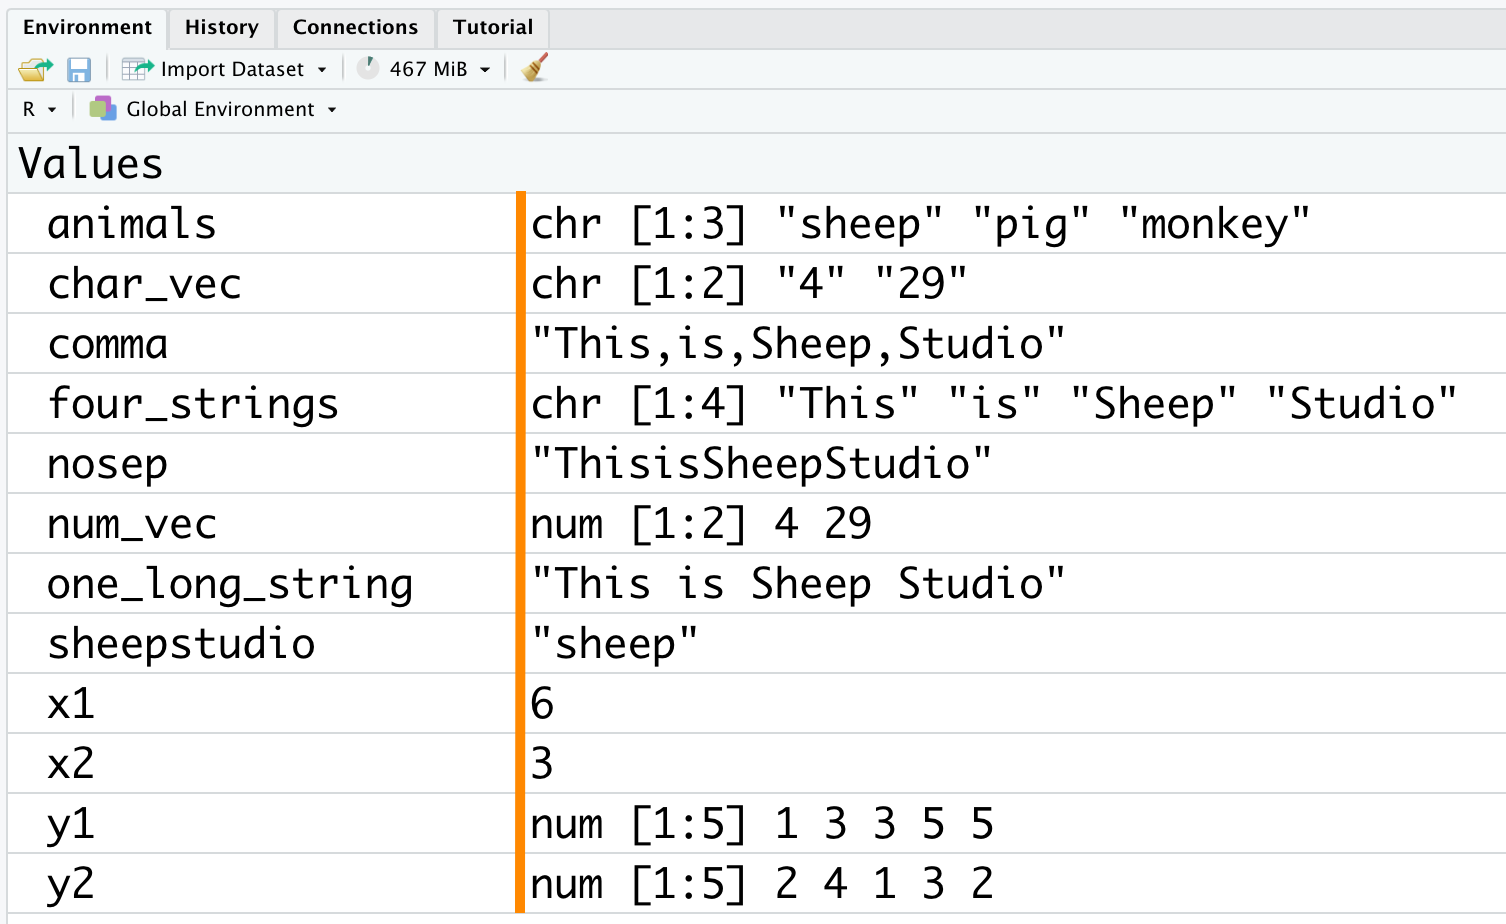
\includegraphics[width=0.7\linewidth]{pics/2enviro} 

}

\caption{Environment}\label{fig:enviro}
\end{figure}

We can see that the environment panel has two columns, with the first column showing the list of object names, and the second column showing the corresponding information for each object. The information includes the vector type (\emph{chr} is short for character and \emph{num} is short for numeric), the vector length, and the first few values of the vector. Note that if the vector is of length 1 (for example \texttt{x1}), the environment will not show the type or the length.

Before introducing the \emph{logical vector}, let's first learn a function called \texttt{is.numeric()}, which checks whether an object is of numeric type,

\begin{Shaded}
\begin{Highlighting}[]
\FunctionTok{is.numeric}\NormalTok{(y1) }\CommentTok{\#Is y1 of numeric type?}
\end{Highlighting}
\end{Shaded}

\begin{verbatim}
#> [1] TRUE
\end{verbatim}

Similar to \texttt{is.numeric()}, you can also use \texttt{is.character()} function to check if the given object is of character type.

\begin{Shaded}
\begin{Highlighting}[]
\FunctionTok{is.character}\NormalTok{(y1) }\CommentTok{\#Is y1 of character type?}
\end{Highlighting}
\end{Shaded}

\begin{verbatim}
#> [1] FALSE
\end{verbatim}

You may notice that results are \texttt{TRUE} or \texttt{FALSE} from the above codes. Actually, \textbf{logical vectors} are vectors that only use \texttt{TRUE} or \texttt{FALSE} as values. Note that \texttt{TRUE} and \texttt{FALSE} are logical constants in R. Similarly, you can use \texttt{is.logical()} to check if the argument is of logical type, or you can use \texttt{class()} to find out the exact type.

\begin{Shaded}
\begin{Highlighting}[]
\NormalTok{logic1 }\OtherTok{\textless{}{-}} \FunctionTok{c}\NormalTok{(}\ConstantTok{TRUE}\NormalTok{, }\ConstantTok{FALSE}\NormalTok{, }\ConstantTok{TRUE}\NormalTok{) }\CommentTok{\#you can also use the c() function to create a logical vector}
\FunctionTok{is.logical}\NormalTok{(logic1)}
\FunctionTok{class}\NormalTok{(logic1)}
\end{Highlighting}
\end{Shaded}

You can also use \texttt{T} to represent \texttt{TRUE} and \texttt{F} to represent \texttt{FALSE} in logical vectors.

\begin{Shaded}
\begin{Highlighting}[]
\NormalTok{logic2 }\OtherTok{\textless{}{-}} \FunctionTok{c}\NormalTok{(T, F, F)}
\FunctionTok{is.logical}\NormalTok{(logic2)}
\FunctionTok{class}\NormalTok{(logic2)}
\end{Highlighting}
\end{Shaded}

It is worth to point out that you don't want to put a pair of double quotes around \texttt{TRUE} or \texttt{FALSE} when you use them as logical values. If you do that, a character vector will be generated instead.

\begin{Shaded}
\begin{Highlighting}[]
\NormalTok{char }\OtherTok{\textless{}{-}} \FunctionTok{c}\NormalTok{(}\StringTok{"TRUE"}\NormalTok{, }\StringTok{"FALSE"}\NormalTok{, }\StringTok{"TRUE"}\NormalTok{)}
\FunctionTok{is.logical}\NormalTok{(char)}
\FunctionTok{class}\NormalTok{(char)}
\end{Highlighting}
\end{Shaded}

Note that the keywords \texttt{TRUE} and \texttt{FALSE} are case sensitive, and all letters inside them need to be in \textbf{upper case}. If you change any letter to the lower case, you will get an error, because \texttt{True} is neither a logical constant nor a defined object.

\begin{Shaded}
\begin{Highlighting}[]
\NormalTok{tlogic }\OtherTok{\textless{}{-}}\NormalTok{ True}
\end{Highlighting}
\end{Shaded}

\begin{verbatim}
#> Error in eval(expr, envir, enclos): object 'True' not found
\end{verbatim}

\hypertarget{the-coercion-rule}{%
\subsection{\texorpdfstring{\textbf{The coercion rule}}{The coercion rule}}\label{the-coercion-rule}}

So far, we have been considering vectors that have values of the same type, namely, numbers, strings, or logical values. In practice, if we have values with a mix of different types in a vector, R will \emph{unify} all values into the most complex one, which is usually called the \textbf{cocercion rule}. Specifically, R use the following order of complexity (from simple to complex).
\[logical < numeric < character\]

Let's see a few examples about the coercion. The first example mixes logical values with numbers.

\begin{Shaded}
\begin{Highlighting}[]
\NormalTok{mix\_1 }\OtherTok{\textless{}{-}} \FunctionTok{c}\NormalTok{(}\ConstantTok{TRUE}\NormalTok{, }\DecValTok{7}\NormalTok{, }\DecValTok{24}\NormalTok{, }\ConstantTok{FALSE}\NormalTok{)}
\NormalTok{mix\_1 }
\end{Highlighting}
\end{Shaded}

\begin{verbatim}
#> [1]  1  7 24  0
\end{verbatim}

\begin{Shaded}
\begin{Highlighting}[]
\FunctionTok{class}\NormalTok{(mix\_1)}
\end{Highlighting}
\end{Shaded}

\begin{verbatim}
#> [1] "numeric"
\end{verbatim}

We can see that \texttt{TRUE} will be converted to 1 and \texttt{FALSE} will be converted to 0 when they appear with numbers.

The second example mixes numbers with strings.

\begin{Shaded}
\begin{Highlighting}[]
\NormalTok{mix\_2 }\OtherTok{\textless{}{-}} \FunctionTok{c}\NormalTok{(}\DecValTok{8}\NormalTok{, }\StringTok{"happy"}\NormalTok{, }\DecValTok{26}\NormalTok{, }\StringTok{"string"}\NormalTok{)}
\NormalTok{mix\_2 }
\end{Highlighting}
\end{Shaded}

\begin{verbatim}
#> [1] "8"      "happy"  "26"     "string"
\end{verbatim}

\begin{Shaded}
\begin{Highlighting}[]
\FunctionTok{class}\NormalTok{(mix\_2)}
\end{Highlighting}
\end{Shaded}

\begin{verbatim}
#> [1] "character"
\end{verbatim}

We can see both 8 and 26 are converted into strings.

The final example mixes logical values, numbers and strings.

\begin{Shaded}
\begin{Highlighting}[]
\NormalTok{mix\_3 }\OtherTok{\textless{}{-}} \FunctionTok{c}\NormalTok{(}\DecValTok{97}\NormalTok{, }\ConstantTok{TRUE}\NormalTok{, }\StringTok{"pig"}\NormalTok{)}
\NormalTok{mix\_3}
\end{Highlighting}
\end{Shaded}

\begin{verbatim}
#> [1] "97"   "TRUE" "pig"
\end{verbatim}

\begin{Shaded}
\begin{Highlighting}[]
\FunctionTok{class}\NormalTok{(mix\_3)}
\end{Highlighting}
\end{Shaded}

\begin{verbatim}
#> [1] "character"
\end{verbatim}

We can see that both 97 and \texttt{TRUE} are converted to strings.

\hypertarget{exercise-2}{%
\subsection{Exercise}\label{exercise-2}}

You can run the following code to do the exercise.

\begin{Shaded}
\begin{Highlighting}[]
\FunctionTok{r02pro}\NormalTok{(}\FloatTok{2.2}\NormalTok{)}
\end{Highlighting}
\end{Shaded}

\hypertarget{vector-patterns}{%
\section{Create Vectors with Patterns}\label{vector-patterns}}

Now you are familiar with numeric vector, character vector and logical vector, and you can create them from scratch using the \texttt{c()} function. However, in many applications, we may want to create vectors with certain patterns. In this section, we will introduce several commonly used functions for generating vectors with patterns.

\hypertarget{create-equally-spaced-numeric-vectors-via}{%
\subsection{\texorpdfstring{Create equally-spaced numeric vectors via \texttt{:}}{Create equally-spaced numeric vectors via :}}\label{create-equally-spaced-numeric-vectors-via}}

One of the commonly used patterns associated with numeric vectors is numeric vectors composed of \textbf{equally-spaced} integers, where the differences between adjacent values in the vectors are all \(1\) or \(-1\).

Suppose we want to create a vector with consecutive integers from 1 to 5. The first method is to write all numbers down in \texttt{c()},

\begin{Shaded}
\begin{Highlighting}[]
\NormalTok{pattern1 }\OtherTok{\textless{}{-}} \FunctionTok{c}\NormalTok{(}\DecValTok{1}\NormalTok{,}\DecValTok{2}\NormalTok{,}\DecValTok{3}\NormalTok{,}\DecValTok{4}\NormalTok{,}\DecValTok{5}\NormalTok{)}
\end{Highlighting}
\end{Shaded}

You can see that it is not too cumbersome to enumerate all 5 integers when creating \texttt{pattern1}. Let's imagine if we want to create a vector containing 100 consecutive integers. Do we have a faster way than writing all 100 integers down? The answer is Yes!

You can use the \textbf{colon operator} \texttt{:}, which is frequently used in everyday programming. (Note that you don't need to use \texttt{c()} with \texttt{:})

\begin{Shaded}
\begin{Highlighting}[]
\NormalTok{pattern2 }\OtherTok{\textless{}{-}} \DecValTok{1}\SpecialCharTok{:}\DecValTok{5} \CommentTok{\#consecutive integers from 1 to 5}
\end{Highlighting}
\end{Shaded}

In addition to creating vectors with consecutive integers that is increasing, \texttt{:} can also be used to create vectors with integers in decreasing sequences.

\begin{Shaded}
\begin{Highlighting}[]
\NormalTok{pattern3 }\OtherTok{\textless{}{-}} \DecValTok{6}\SpecialCharTok{:}\DecValTok{2}  \CommentTok{\#decreasing sequence from 6 to 2}
\NormalTok{pattern4 }\OtherTok{\textless{}{-}} \DecValTok{3}\SpecialCharTok{:{-}}\DecValTok{3} \CommentTok{\#decreasing sequence from 3 to {-}3}
\end{Highlighting}
\end{Shaded}

Powerful the \texttt{:} operator is, it can only generate equally-spaced numeric vectors with increment 1 or -1. If you want to generate numeric vectors with different increments, you can use the more powerful \texttt{seq()} function.

\hypertarget{create-equally-spaced-numeric-vectors-via-seq}{%
\subsection{\texorpdfstring{Create equally-spaced numeric vectors via \texttt{seq()}}{Create equally-spaced numeric vectors via seq()}}\label{create-equally-spaced-numeric-vectors-via-seq}}

A very efficient way to create \textbf{equally-spaced} numeric vectors is to use the \texttt{seq()} function, which is short for sequence.

\textbf{\emph{a. Create sequences with \texttt{by} argument}}

To use the \texttt{seq()} function, you can specify the start value of the sequence in the \texttt{from} argument, the limit end value in the \texttt{to} argument, and the increment in the \texttt{by} argument.

\begin{Shaded}
\begin{Highlighting}[]
\FunctionTok{seq}\NormalTok{(}\AttributeTok{from =} \DecValTok{1}\NormalTok{, }\AttributeTok{to =} \DecValTok{5}\NormalTok{, }\AttributeTok{by =} \DecValTok{1}\NormalTok{)}
\end{Highlighting}
\end{Shaded}

Here, the vector starts with 1, increases by 1 at each step, and ends at 5. Note that the \texttt{from} and \texttt{by} arguments are optional in \texttt{seq()}. If you don't specify their values, \texttt{seq()} will use the default value 1 for both arguments.

\begin{Shaded}
\begin{Highlighting}[]
\FunctionTok{seq}\NormalTok{(}\AttributeTok{to =} \DecValTok{5}\NormalTok{)}
\end{Highlighting}
\end{Shaded}

\begin{infobox}{caution}

Now you have had four methods to create vectors with consecutive integers.

\begin{Shaded}
\begin{Highlighting}[]
\FunctionTok{c}\NormalTok{(}\DecValTok{1}\NormalTok{,}\DecValTok{2}\NormalTok{,}\DecValTok{3}\NormalTok{,}\DecValTok{4}\NormalTok{,}\DecValTok{5}\NormalTok{,}\DecValTok{6}\NormalTok{)                }\CommentTok{\#write all numbers down}
\DecValTok{1}\SpecialCharTok{:}\DecValTok{6}                           \CommentTok{\#use colon operator}
\FunctionTok{seq}\NormalTok{(}\AttributeTok{from =} \DecValTok{1}\NormalTok{, }\AttributeTok{to =} \DecValTok{6}\NormalTok{, }\AttributeTok{by =} \DecValTok{1}\NormalTok{) }\CommentTok{\#use seq()}
\FunctionTok{seq}\NormalTok{(}\AttributeTok{to =} \DecValTok{6}\NormalTok{)                   }\CommentTok{\#use seq()}
\end{Highlighting}
\end{Shaded}

\end{infobox}

Next, let's change the increment to 2 and you will get a numeric vector with 1, 3 and 5 as its values.

\begin{Shaded}
\begin{Highlighting}[]
\FunctionTok{seq}\NormalTok{(}\AttributeTok{from =} \DecValTok{1}\NormalTok{, }\AttributeTok{to =} \DecValTok{5}\NormalTok{, }\AttributeTok{by =} \DecValTok{2}\NormalTok{)}
\end{Highlighting}
\end{Shaded}

\begin{verbatim}
#> [1] 1 3 5
\end{verbatim}

If you only change the limit end value to 6, you still get the same sequence, since the next value in the sequence would be 7 which is larger than the limit end value 6.

\begin{Shaded}
\begin{Highlighting}[]
\FunctionTok{seq}\NormalTok{(}\AttributeTok{from =} \DecValTok{1}\NormalTok{, }\AttributeTok{to =} \DecValTok{6}\NormalTok{, }\AttributeTok{by =} \DecValTok{2}\NormalTok{) }
\end{Highlighting}
\end{Shaded}

\begin{verbatim}
#> [1] 1 3 5
\end{verbatim}

Unlike \texttt{:}, you can set values of three arguments in \texttt{seq()} as decimal numbers. Here, you will get a sequence starting with 1.1, each element in this sequence will be added by 0.7 on the basis of the previous element, until the biggest number smaller than 6.2.

\begin{Shaded}
\begin{Highlighting}[]
\FunctionTok{seq}\NormalTok{(}\AttributeTok{from =} \FloatTok{1.1}\NormalTok{, }\AttributeTok{to =} \FloatTok{6.2}\NormalTok{, }\AttributeTok{by =} \FloatTok{0.7}\NormalTok{) }
\end{Highlighting}
\end{Shaded}

\begin{verbatim}
#> [1] 1.1 1.8 2.5 3.2 3.9 4.6 5.3 6.0
\end{verbatim}

You can also create a decreasing sequence by using a smaller \texttt{to} value than the \texttt{from} value, coupled with a negative value in the \texttt{by} argument.

\begin{Shaded}
\begin{Highlighting}[]
\FunctionTok{seq}\NormalTok{(}\AttributeTok{from =} \FloatTok{1.5}\NormalTok{, }\AttributeTok{to =} \SpecialCharTok{{-}}\DecValTok{1}\NormalTok{, }\AttributeTok{by =} \SpecialCharTok{{-}}\FloatTok{0.5}\NormalTok{) }
\end{Highlighting}
\end{Shaded}

If a positive value is used in the \texttt{by} argument in a decreasing sequence, you will see an error message.

\begin{Shaded}
\begin{Highlighting}[]
\FunctionTok{seq}\NormalTok{(}\AttributeTok{from =} \FloatTok{1.5}\NormalTok{, }\AttributeTok{to =} \SpecialCharTok{{-}}\DecValTok{1}\NormalTok{, }\AttributeTok{by =} \FloatTok{0.5}\NormalTok{) }
\end{Highlighting}
\end{Shaded}

\begin{verbatim}
#> Error in seq.default(from = 1.5, to = -1, by = 0.5): wrong sign in 'by' argument
\end{verbatim}

\textbf{\emph{b. Create sequences with \texttt{length.out} argument}}

Instead of setting the increment, you can also specify the \texttt{length.out} argument, which creates a sequence with equal space in the specified length. R will automatically calculate the interval between two neighboring numbers according to values of three arguments in \texttt{seq()}.

\begin{Shaded}
\begin{Highlighting}[]
\FunctionTok{seq}\NormalTok{(}\AttributeTok{from =} \DecValTok{1}\NormalTok{, }\AttributeTok{to =} \DecValTok{5}\NormalTok{, }\AttributeTok{length.out =} \DecValTok{9}\NormalTok{) }
\end{Highlighting}
\end{Shaded}

Here, you will get a sequence of length 9 from 1 to 5.

You can also create a decreasing sequence by using the \texttt{length.out} argument.

\begin{Shaded}
\begin{Highlighting}[]
\FunctionTok{seq}\NormalTok{(}\AttributeTok{from =} \DecValTok{5}\NormalTok{, }\AttributeTok{to =} \SpecialCharTok{{-}}\DecValTok{5}\NormalTok{, }\AttributeTok{length.out =} \DecValTok{9}\NormalTok{) }
\end{Highlighting}
\end{Shaded}

\begin{infobox}{caution}
Unlike creating sequences with \texttt{by} argument, if you specify the \texttt{length.out} argument in \texttt{seq()}, the start value and end value of the sequence you get will be exactly match the input arguments.

\end{infobox}

\textbf{\emph{c.~Create sequences with both \texttt{by} and \texttt{length.out} arguments}}

Lastly, if you provide both the \texttt{by} and \texttt{length.out} arguments, only one of \texttt{from} and \texttt{to} is needed. With one value (the start value or the limit end value) fixed, \texttt{seq()} will create a vector with specified increment and length.

If you only have the \texttt{from} argument, you will get a sequence starting from the value you set with the increment in the \texttt{by} argument, until you get a sequence with specified length.

\begin{Shaded}
\begin{Highlighting}[]
\FunctionTok{seq}\NormalTok{(}\AttributeTok{from =} \DecValTok{1}\NormalTok{, }\AttributeTok{by =} \DecValTok{2}\NormalTok{, }\AttributeTok{length.out =} \DecValTok{5}\NormalTok{)}
\end{Highlighting}
\end{Shaded}

If you only have the \texttt{to} argument, you will get a sequence end with the value you set with the increment in the \texttt{by} argument, until you get a sequence with specified length.

\begin{Shaded}
\begin{Highlighting}[]
\FunctionTok{seq}\NormalTok{(}\AttributeTok{to =} \DecValTok{1}\NormalTok{, }\AttributeTok{by =} \DecValTok{2}\NormalTok{, }\AttributeTok{length.out =} \DecValTok{5}\NormalTok{)}
\end{Highlighting}
\end{Shaded}

One last thing regarding \texttt{seq()} is that you can \emph{at most} provide three arguments. For example, you will see an error when running the following example since all four arguments are specified.

\begin{Shaded}
\begin{Highlighting}[]
\FunctionTok{seq}\NormalTok{(}\AttributeTok{from =} \DecValTok{1}\NormalTok{, }\AttributeTok{to =} \DecValTok{3}\NormalTok{, }\AttributeTok{by =} \DecValTok{1}\NormalTok{, }\AttributeTok{length.out =} \DecValTok{3}\NormalTok{)}
\end{Highlighting}
\end{Shaded}

\begin{verbatim}
#> Error in seq.default(from = 1, to = 3, by = 1, length.out = 3): too many arguments
\end{verbatim}

\hypertarget{create-a-matching-numeric-vectors-via-seq_along}{%
\subsection{\texorpdfstring{Create a matching numeric vectors via \texttt{seq\_along()}}{Create a matching numeric vectors via seq\_along()}}\label{create-a-matching-numeric-vectors-via-seq_along}}

Now, we introduce one function related to \texttt{seq()}. Let's first create a numeric vector,

\begin{Shaded}
\begin{Highlighting}[]
\NormalTok{extend }\OtherTok{\textless{}{-}} \FunctionTok{seq}\NormalTok{(}\AttributeTok{from =} \DecValTok{2}\NormalTok{, }\AttributeTok{to =} \DecValTok{8}\NormalTok{, }\AttributeTok{length.out =} \DecValTok{9}\NormalTok{) }
\end{Highlighting}
\end{Shaded}

From the \texttt{seq()} above, you know that the length of this vector is \texttt{9}. Next, let's put this numeric vector in \texttt{seq\_along()}.

\begin{Shaded}
\begin{Highlighting}[]
\FunctionTok{seq\_along}\NormalTok{(extend)}
\end{Highlighting}
\end{Shaded}

\begin{verbatim}
#> [1] 1 2 3 4 5 6 7 8 9
\end{verbatim}

\texttt{seq\_along()} takes a vector as its argument, and generates consecutive integers from 1 to the length of the input vector. The \texttt{seq\_along()} function is commonly used when writing loops, which will be covered at a later time.

\begin{infobox}{caution}

You can also use \texttt{1:length(extend)} to get the same result as \texttt{seq\_along(extend)}.

\begin{Shaded}
\begin{Highlighting}[]
\DecValTok{1}\SpecialCharTok{:}\FunctionTok{length}\NormalTok{(extend)}
\end{Highlighting}
\end{Shaded}

\end{infobox}

\hypertarget{create-numeric-vectors-via-sequence}{%
\subsection{\texorpdfstring{Create numeric vectors via \texttt{sequence()}}{Create numeric vectors via sequence()}}\label{create-numeric-vectors-via-sequence}}

Sometimes, you may want to combine multiple equally-spaced integer sequences into a single vector. To do this, you can use the function \texttt{sequence()}. The most common usage of \texttt{sequence()} is to supply a vector of integers as its input.

\begin{Shaded}
\begin{Highlighting}[]
\NormalTok{comp\_seq1 }\OtherTok{\textless{}{-}} \FunctionTok{sequence}\NormalTok{(}\FunctionTok{c}\NormalTok{(}\DecValTok{2}\NormalTok{, }\DecValTok{3}\NormalTok{, }\DecValTok{5}\NormalTok{)) }
\NormalTok{comp\_seq1}
\end{Highlighting}
\end{Shaded}

\begin{verbatim}
#>  [1] 1 2 1 2 3 1 2 3 4 5
\end{verbatim}

From the result, we can see that it firstly create equally-spaced vectors 1:2, 1:3, and 1:5, then combine all vectors into a single one. This avoids the trouble of writing something like \texttt{c(1:2,\ 1:3,\ 1:5)}.

More generally, we can construct a vector of more complex integer sequences with additional arguments, namely \texttt{sequence(nvec,\ from,\ by)}. Here, the \texttt{nvec} , \texttt{from} and \texttt{by} are integer vectors of the corresponding \texttt{length.out}, \texttt{from}, and \texttt{by} arguments of each equally-spaced sequence. Let's see the following example.

\begin{Shaded}
\begin{Highlighting}[]
\NormalTok{comp\_seq2 }\OtherTok{\textless{}{-}} \FunctionTok{sequence}\NormalTok{(}\AttributeTok{nvec =} \FunctionTok{c}\NormalTok{(}\DecValTok{4}\NormalTok{, }\DecValTok{3}\NormalTok{, }\DecValTok{2}\NormalTok{), }\AttributeTok{from =} \FunctionTok{c}\NormalTok{(}\DecValTok{1}\NormalTok{, }\DecValTok{2}\NormalTok{, }\SpecialCharTok{{-}}\DecValTok{1}\NormalTok{), }\AttributeTok{by =} \FunctionTok{c}\NormalTok{(}\DecValTok{2}\NormalTok{, }\SpecialCharTok{{-}}\DecValTok{1}\NormalTok{, }\DecValTok{2}\NormalTok{))}
\NormalTok{comp\_seq2}
\end{Highlighting}
\end{Shaded}

\begin{verbatim}
#> [1]  1  3  5  7  2  1  0 -1  1
\end{verbatim}

Now, \texttt{sequence()} generate three different equally-spaced integer sequences and combine them to a single vector. We can reproduce the vector using \texttt{c()} and three calls of the \texttt{seq()} function.

\begin{Shaded}
\begin{Highlighting}[]
\NormalTok{comp\_seq3 }\OtherTok{\textless{}{-}} \FunctionTok{c}\NormalTok{(}\FunctionTok{seq}\NormalTok{(}\AttributeTok{from =} \DecValTok{1}\NormalTok{,  }\AttributeTok{by =}  \DecValTok{2}\NormalTok{, }\AttributeTok{length.out =} \DecValTok{4}\NormalTok{),}
               \FunctionTok{seq}\NormalTok{(}\AttributeTok{from =} \DecValTok{2}\NormalTok{,  }\AttributeTok{by =} \SpecialCharTok{{-}}\DecValTok{1}\NormalTok{, }\AttributeTok{length.out =} \DecValTok{3}\NormalTok{),}
               \FunctionTok{seq}\NormalTok{(}\AttributeTok{from =} \SpecialCharTok{{-}}\DecValTok{1}\NormalTok{, }\AttributeTok{by =}  \DecValTok{2}\NormalTok{, }\AttributeTok{length.out =} \DecValTok{2}\NormalTok{))}
\NormalTok{comp\_seq3}
\end{Highlighting}
\end{Shaded}

\begin{verbatim}
#> [1]  1  3  5  7  2  1  0 -1  1
\end{verbatim}

\hypertarget{create-numeric-character-and-logical-vectors-with-repetition}{%
\subsection{Create numeric, character and logical vectors with repetition}\label{create-numeric-character-and-logical-vectors-with-repetition}}

Another commonly used pattern associated with vectors is \textbf{repetition}. Note that while the equally-spaced pattern only makes sense for numeric vectors, the repetition pattern work for all three kinds of vectors.

To do repetition, you can use the \texttt{rep()} function, which works by repeating the first argument for the number of times indicated in the second argument.

Firstly, let's create a numeric vector with repetition.

\begin{Shaded}
\begin{Highlighting}[]
\NormalTok{num1 }\OtherTok{\textless{}{-}} \FunctionTok{rep}\NormalTok{(}\DecValTok{2}\NormalTok{, }\DecValTok{4}\NormalTok{)}
\NormalTok{num1}
\end{Highlighting}
\end{Shaded}

\begin{verbatim}
#> [1] 2 2 2 2
\end{verbatim}

Since the first argument is 2 and the second argument is 4, 2 is repeated for 4 times, resulting a length-4 vector with all elements 2.

The first argument can also be a numeric vector with several values.

\begin{Shaded}
\begin{Highlighting}[]
\NormalTok{num2 }\OtherTok{\textless{}{-}} \FunctionTok{rep}\NormalTok{(}\FunctionTok{c}\NormalTok{(}\DecValTok{1}\NormalTok{, }\DecValTok{4}\NormalTok{, }\DecValTok{2}\NormalTok{), }\DecValTok{3}\NormalTok{)}
\NormalTok{num2}
\end{Highlighting}
\end{Shaded}

\begin{verbatim}
#> [1] 1 4 2 1 4 2 1 4 2
\end{verbatim}

Here, then \texttt{rep()} will repeat the whole vector \texttt{c(1,\ 4,\ 2)} three times. Note that the vector is \textbf{repeated as a whole}, not elementwisely.

You may be wondering what happens the second argument also has several numbers? Let's try together.

\begin{Shaded}
\begin{Highlighting}[]
\NormalTok{num3 }\OtherTok{\textless{}{-}} \FunctionTok{rep}\NormalTok{(}\FunctionTok{c}\NormalTok{(}\DecValTok{1}\NormalTok{,}\DecValTok{5}\NormalTok{,}\DecValTok{7}\NormalTok{), }\FunctionTok{c}\NormalTok{(}\DecValTok{3}\NormalTok{,}\DecValTok{2}\NormalTok{,}\DecValTok{1}\NormalTok{))}
\NormalTok{num3}
\end{Highlighting}
\end{Shaded}

\begin{verbatim}
#> [1] 1 1 1 5 5 7
\end{verbatim}

When the second argument is also a vector, R will do an \textbf{element repeat} operation by repeating each element in the first argument the number of times indicated in the corresponding location of the second argument, and combine the repeated vectors to a single vector. In this example, 1 is repeated 3 times, 5 is repeated twice, and 7 is repeated once. It is equivalent to

\begin{Shaded}
\begin{Highlighting}[]
\FunctionTok{c}\NormalTok{(}\FunctionTok{rep}\NormalTok{(}\DecValTok{1}\NormalTok{,}\DecValTok{3}\NormalTok{), }\FunctionTok{rep}\NormalTok{(}\DecValTok{4}\NormalTok{,}\DecValTok{2}\NormalTok{), }\FunctionTok{rep}\NormalTok{(}\DecValTok{7}\NormalTok{,}\DecValTok{1}\NormalTok{))}
\end{Highlighting}
\end{Shaded}

The \texttt{rep()} function works the same way if the first argument is a character vector.

\begin{Shaded}
\begin{Highlighting}[]
\NormalTok{animals1 }\OtherTok{\textless{}{-}} \FunctionTok{rep}\NormalTok{(}\FunctionTok{c}\NormalTok{(}\StringTok{"sheep"}\NormalTok{, }\StringTok{"pig"}\NormalTok{, }\StringTok{"monkey"}\NormalTok{), }\DecValTok{2}\NormalTok{)}
\NormalTok{animals1}
\NormalTok{animals2 }\OtherTok{\textless{}{-}} \FunctionTok{rep}\NormalTok{(}\FunctionTok{c}\NormalTok{(}\StringTok{"sheep"}\NormalTok{, }\StringTok{"pig"}\NormalTok{, }\StringTok{"monkey"}\NormalTok{), }\FunctionTok{c}\NormalTok{(}\DecValTok{3}\NormalTok{, }\DecValTok{2}\NormalTok{, }\DecValTok{1}\NormalTok{))}
\NormalTok{animals2}
\end{Highlighting}
\end{Shaded}

You can also use logical vectors in the first argument.

\begin{Shaded}
\begin{Highlighting}[]
\NormalTok{logic }\OtherTok{\textless{}{-}} \FunctionTok{rep}\NormalTok{(}\FunctionTok{c}\NormalTok{(}\ConstantTok{TRUE}\NormalTok{, }\ConstantTok{FALSE}\NormalTok{), }\FunctionTok{c}\NormalTok{(}\DecValTok{3}\NormalTok{,}\DecValTok{2}\NormalTok{))}
\NormalTok{logic}
\end{Highlighting}
\end{Shaded}

\hypertarget{getting-unique-elements-and-their-frequencies}{%
\subsection{Getting unique elements and their frequencies}\label{getting-unique-elements-and-their-frequencies}}

So far, you have learned how to create vectors with different patterns. Sometimes, you may want to get the unique elements of a vector and their corresponding frequencies. Let's use \texttt{num3} as an example. \textbf{(Don't forget to use \texttt{ls()} or check the environment panel to find all objects you have defined)},

\begin{Shaded}
\begin{Highlighting}[]
\NormalTok{num3           }\CommentTok{\#check the values}
\end{Highlighting}
\end{Shaded}

\begin{verbatim}
#> [1] 1 1 1 5 5 7
\end{verbatim}

You can use \texttt{unique()} to show all unique elements in vectors

\begin{Shaded}
\begin{Highlighting}[]
\FunctionTok{unique}\NormalTok{(num3)   }\CommentTok{\#get the unique elements}
\end{Highlighting}
\end{Shaded}

\begin{verbatim}
#> [1] 1 5 7
\end{verbatim}

From the result, you know the unique elements in \texttt{num3} are \texttt{1},\texttt{5}, and \texttt{7}. To get the frequency of each element, you can use the \texttt{table()} function.

\begin{Shaded}
\begin{Highlighting}[]
\FunctionTok{table}\NormalTok{(num3)    }\CommentTok{\#get the frequency table}
\end{Highlighting}
\end{Shaded}

\begin{verbatim}
#> num3
#> 1 5 7 
#> 3 2 1
\end{verbatim}

Here, the first row is the name of the object, the second row shows all unique elements, and the third row is the corresponding frequency of each element in the same column. In \texttt{num3}, there are three \texttt{1}s, two \texttt{5}s and one \texttt{7}.

\texttt{unique()} and \texttt{table()} work similarly for character vectors and logical vectors. You can try the following codes.

\begin{Shaded}
\begin{Highlighting}[]
\NormalTok{animals}
\FunctionTok{unique}\NormalTok{(animals)}
\FunctionTok{table}\NormalTok{(animals)}
\NormalTok{logic}
\FunctionTok{unique}\NormalTok{(logic)}
\FunctionTok{table}\NormalTok{(logic)}
\end{Highlighting}
\end{Shaded}

\hypertarget{exercise-3}{%
\subsection{Exercise}\label{exercise-3}}

You can run the following code to do the exercise.

\begin{Shaded}
\begin{Highlighting}[]
\FunctionTok{r02pro}\NormalTok{(}\FloatTok{2.3}\NormalTok{)}
\end{Highlighting}
\end{Shaded}

\hypertarget{sort-vector}{%
\section{Sort, Rank, \& Order}\label{sort-vector}}

In the past two sections, you have mastered how to create vectors of different types including numeric, character and logical. In addition, you know how to create vectors with patterns. A vector usually contains more than one elements. Sometimes, you want to order the elements in various ways. In this section, we will introduce important functions that relate to ordering elements in a vector.

\hypertarget{numeric-vectors}{%
\subsection{Numeric vectors}\label{numeric-vectors}}

Let's start with numeric vectors. Firstly, let's create a numeric vector which will be used throughout this section.

\begin{Shaded}
\begin{Highlighting}[]
\NormalTok{x }\OtherTok{\textless{}{-}} \FunctionTok{c}\NormalTok{(}\DecValTok{2}\NormalTok{, }\DecValTok{3}\NormalTok{, }\DecValTok{2}\NormalTok{, }\DecValTok{0}\NormalTok{, }\DecValTok{4}\NormalTok{, }\DecValTok{7}\NormalTok{) }
\NormalTok{x }\CommentTok{\#check the value of x}
\end{Highlighting}
\end{Shaded}

\textbf{\emph{a. Sort vectors}}

The first function we will introduce is \texttt{sort()}. By default, the \texttt{sort()} function \textbf{sorts} elements in vector in the ascending order, namely from the smallest to largest.

\begin{Shaded}
\begin{Highlighting}[]
\FunctionTok{sort}\NormalTok{(x)}
\end{Highlighting}
\end{Shaded}

\begin{verbatim}
#> [1] 0 2 2 3 4 7
\end{verbatim}

If you want to sort the vector in the descending order, namely from the largest to smallest, you can set a second argument \texttt{decreasing\ =\ TRUE}.

\begin{Shaded}
\begin{Highlighting}[]
\FunctionTok{sort}\NormalTok{(x, }\AttributeTok{decreasing =} \ConstantTok{TRUE}\NormalTok{)}
\end{Highlighting}
\end{Shaded}

\begin{verbatim}
#> [1] 7 4 3 2 2 0
\end{verbatim}

\textbf{\emph{b. Ranks of vectors}}

Next, let's talk about ranks. The \texttt{rank()} function gives the \textbf{ranks} for each element of the vector, namely the corresponding positions in the \textbf{ascending order}.

\begin{Shaded}
\begin{Highlighting}[]
\FunctionTok{rank}\NormalTok{(x)}
\end{Highlighting}
\end{Shaded}

\begin{verbatim}
#> [1] 2.5 4.0 2.5 1.0 5.0 6.0
\end{verbatim}

If you check the value of \texttt{x}, you can see that the smallest value of \texttt{x} is 0, which corresponds to the fourth element. Thus, the fourth element has rank 1. The second smallest value of \texttt{x} is 2, which is shared at the first and the third elements, resulting a \textbf{tie} (elements with the same value will result in a tie). Normally, these two elements would have ranks 2 and 3. To break the tie, the \texttt{rank()} function assigns all the elements involving in the tie (the first and third elements in this example) the same rank, which is average of all their ranks (the average of 2 and 3), by default. In addition to this default behavior for handling ties, \texttt{rank()} also provides other options by setting the \texttt{ties.method} argument.

If you set \texttt{ties.method\ =\ "min"}, all the tied elements will have the \emph{minimum rank} instead of the average rank. In this case, the minimum rank is 2.

\begin{Shaded}
\begin{Highlighting}[]
\FunctionTok{rank}\NormalTok{(x, }\AttributeTok{ties.method =} \StringTok{"min"}\NormalTok{)}
\end{Highlighting}
\end{Shaded}

\begin{verbatim}
#> [1] 2 4 2 1 5 6
\end{verbatim}

If you want to break the ties by the order it appears in the vector, you can set \texttt{ties.method\ =\ "first"}. Then the earlier appearing elements will have smaller ranks than the later ones. In this example, the first element will have rank 2 and the third element has rank 3, since the first element appears earlier than the third element. There are other options for handling ties, which you can look up in the documentaion of \texttt{rank()} if interested.

\begin{Shaded}
\begin{Highlighting}[]
\FunctionTok{rank}\NormalTok{(x, }\AttributeTok{ties.method =} \StringTok{"first"}\NormalTok{)}
\end{Highlighting}
\end{Shaded}

\begin{verbatim}
#> [1] 2 4 3 1 5 6
\end{verbatim}

\begin{infobox}{caution}
Unlike \texttt{sort()}, you can't get positions in the descending order from the \texttt{rank()} function, which means you can't add \texttt{decreasing\ =\ TRUE} in \texttt{rank()}.

\end{infobox}

\textbf{\emph{c.~Order of vectors}}

The next item we want to introduce is the \texttt{order()} function. Note that the function name order could be a bit misleading since ordering elements also has the same meaning of sorting. However, although it is related to sorting, it is a very \emph{different} function from \texttt{sort()}.

Let's recall the values of \texttt{x} and apply \texttt{order()} to \texttt{x}.

\begin{Shaded}
\begin{Highlighting}[]
\NormalTok{x}
\end{Highlighting}
\end{Shaded}

\begin{verbatim}
#> [1] 2 3 2 0 4 7
\end{verbatim}

\begin{Shaded}
\begin{Highlighting}[]
\FunctionTok{order}\NormalTok{(x)}
\end{Highlighting}
\end{Shaded}

\begin{verbatim}
#> [1] 4 1 3 2 5 6
\end{verbatim}

From the result, you can see that the \texttt{order()} function returns \textbf{indices} for the elements in the ascending order, namely from the smallest to the largest. For example, the first output is 4, indicating the 4th element in \texttt{x} is the smallest. The second output is 1, showing the 1st element in \texttt{x} is the second smallest.

\begin{infobox}{caution}
Unlike \texttt{rank()}, the \texttt{order()} function breaks the ties by the appearing order by default.

\end{infobox}

If you want the indices corresponding to the descending order, then you can set \texttt{decreasing\ =\ TRUE} just like what we did in the \texttt{sort()} function.

\begin{Shaded}
\begin{Highlighting}[]
\FunctionTok{order}\NormalTok{(x, }\AttributeTok{decreasing =} \ConstantTok{TRUE}\NormalTok{)  }
\end{Highlighting}
\end{Shaded}

So far, we have covered \texttt{sort()}, \texttt{rank()} and \texttt{order()} functions for numeric vectors. It is helpful to provide a brief summary.

\begin{itemize}
\tightlist
\item
  The \texttt{sort()} function sorts elements in vectors.
\item
  The \texttt{rank()} function will give ranks for each element of the vector.
\item
  The \texttt{order()} function returns indices for the elements.
\end{itemize}

\hypertarget{character-vectors}{%
\subsection{Character vectors}\label{character-vectors}}

Now, let's move to character vectors. For character vectors, R uses the \textbf{lexicographical ordering}, which is sometimes called dictionary order since it is the order used in a dictionary. Similar to numeric vectors, let's first prepare a character vector. Note that the strings in character vectors can contain letters, numbers, or symbols.

\begin{Shaded}
\begin{Highlighting}[]
\NormalTok{char\_vec }\OtherTok{\textless{}{-}} \FunctionTok{c}\NormalTok{(}\StringTok{"a"}\NormalTok{, }\StringTok{"A"}\NormalTok{, }\StringTok{"B"}\NormalTok{, }\StringTok{"b"}\NormalTok{, }\StringTok{"ab"}\NormalTok{,}\StringTok{"aC"}\NormalTok{, }\StringTok{"1c"}\NormalTok{, }\StringTok{".a"}\NormalTok{, }\StringTok{"1a"}\NormalTok{,}\StringTok{"2a"}\NormalTok{,}\StringTok{".a"}\NormalTok{,}\StringTok{"\&u"}\NormalTok{,}\StringTok{"3"}\NormalTok{,}\StringTok{"\_4"}\NormalTok{)}
\end{Highlighting}
\end{Shaded}

\textbf{\emph{a. Ordering rules}}

First, let's discuss the ordering of a single character, including symbols, digits and letters.
There are a few important ordering rules as follows.

\begin{itemize}
\tightlist
\item
  symbols \textless{} digits \textless{} letters: symbols appears first, followed by digits, and letters come last.
\item
  symbols are ordered in the following way.
\end{itemize}

\begin{Shaded}
\begin{Highlighting}[]
\NormalTok{syms }\OtherTok{\textless{}{-}} \FunctionTok{c}\NormalTok{(}\StringTok{" "}\NormalTok{,}\StringTok{","}\NormalTok{,}\StringTok{";"}\NormalTok{,}\StringTok{"\_"}\NormalTok{,}\StringTok{"("}\NormalTok{,}\StringTok{")"}\NormalTok{,}\StringTok{"!"}\NormalTok{,}\StringTok{"["}\NormalTok{,}\StringTok{"]"}\NormalTok{,}\StringTok{"\{"}\NormalTok{,}\StringTok{"\}"}\NormalTok{,}\StringTok{"{-}"}\NormalTok{,}\StringTok{"*"}\NormalTok{,}\StringTok{"/"}\NormalTok{,}\StringTok{"\#"}\NormalTok{,}\StringTok{"$"}\NormalTok{,}\StringTok{"\%"}\NormalTok{,}\StringTok{"\^{}"}\NormalTok{,}\StringTok{"\&"}\NormalTok{,}\StringTok{"\textasciigrave{}"}\NormalTok{,}\StringTok{"@"}\NormalTok{,}\StringTok{"+"}\NormalTok{,}\StringTok{"="}\NormalTok{,}\StringTok{"|"}\NormalTok{,}\StringTok{"?"}\NormalTok{,}\StringTok{"\textless{}"}\NormalTok{,}\StringTok{"\textgreater{}"}\NormalTok{,}\StringTok{"."}\NormalTok{)}
\FunctionTok{sort}\NormalTok{(syms)}
\end{Highlighting}
\end{Shaded}

\begin{verbatim}
#>  [1] " " "_" "-" "," ";" "!" "?" "." "(" ")" "[" "]" "{" "}" "@" "*" "/" "&" "#"
#> [20] "%" "`" "^" "+" "<" "=" ">" "|" "$"
\end{verbatim}

\begin{itemize}
\tightlist
\item
  digits are in an ascending order: the smaller digits appear earlier than the bigger ones.
\end{itemize}

\begin{Shaded}
\begin{Highlighting}[]
\NormalTok{nums }\OtherTok{\textless{}{-}} \DecValTok{0}\SpecialCharTok{:}\DecValTok{9}
\FunctionTok{sort}\NormalTok{(nums)}
\end{Highlighting}
\end{Shaded}

\begin{verbatim}
#>  [1] 0 1 2 3 4 5 6 7 8 9
\end{verbatim}

\begin{itemize}
\tightlist
\item
  letters are alphabetically ordered: for the same letter,the lower case comes first
  \(a<A<b<B<\cdots<z<Z\).
\end{itemize}

\begin{Shaded}
\begin{Highlighting}[]
\NormalTok{lower\_letters }\OtherTok{\textless{}{-}}\NormalTok{ letters}
\NormalTok{upper\_letters }\OtherTok{\textless{}{-}}\NormalTok{ LETTERS}
\NormalTok{all\_letters }\OtherTok{\textless{}{-}} \FunctionTok{c}\NormalTok{(lower\_letters,upper\_letters)}
\FunctionTok{sort}\NormalTok{(all\_letters)}
\end{Highlighting}
\end{Shaded}

\begin{verbatim}
#>  [1] "a" "A" "b" "B" "c" "C" "d" "D" "e" "E" "f" "F" "g" "G" "h" "H" "i" "I" "j"
#> [20] "J" "k" "K" "l" "L" "m" "M" "n" "N" "o" "O" "p" "P" "q" "Q" "r" "R" "s" "S"
#> [39] "t" "T" "u" "U" "v" "V" "w" "W" "x" "X" "y" "Y" "z" "Z"
\end{verbatim}

You can combine symbols, numbers and letters into a single vector and get the order.

\begin{Shaded}
\begin{Highlighting}[]
\NormalTok{all\_chars }\OtherTok{\textless{}{-}} \FunctionTok{c}\NormalTok{(syms, nums, all\_letters)}
\FunctionTok{sort}\NormalTok{(all\_chars)}
\end{Highlighting}
\end{Shaded}

\textbf{\emph{b. Sort vectors}}

As before, you can apply \texttt{sort()} on character vectors. Basically, it orders by the first character, moves to the second character if there are ties in the first character (same first character), and look at more characters until the ties are broken or run out of characters.

\begin{Shaded}
\begin{Highlighting}[]
\FunctionTok{sort}\NormalTok{(char\_vec)}
\end{Highlighting}
\end{Shaded}

\begin{verbatim}
#>  [1] "_4" ".a" ".a" "&u" "1a" "1c" "2a" "3"  "a"  "A"  "ab" "aC" "b"  "B"
\end{verbatim}

We have the following observations.

\begin{itemize}
\tightlist
\item
  According to the ordering rule of symbols, \texttt{\_4} is the first, \texttt{.a} should be the second and \texttt{\&u} is the third.
\item
  \texttt{1a} and \texttt{1c} have the same first character, since a comes before c, \texttt{1a} comes before \texttt{1c}.
\item
  \texttt{ab} and \texttt{aC} have the same first character, since b comes before C (regardless of the case), \texttt{ab} comes before \texttt{aC}.
\end{itemize}

Of course, we can also have the order reversed by setting \texttt{decreasing\ =\ TRUE}.

\begin{Shaded}
\begin{Highlighting}[]
\FunctionTok{sort}\NormalTok{(char\_vec, }\AttributeTok{decreasing =} \ConstantTok{TRUE}\NormalTok{)}
\end{Highlighting}
\end{Shaded}

\textbf{\emph{c.~Ranks of vectors}}

Similarly, you can look at the ranks for each element according to the ordering rules. Here, the element with rank 1 is \texttt{\_4} and \texttt{.a} has rank 2. Just like numeric vectors, if you have elements with the same value in character vectors, the rank of these elements will be the same (the average of the corresponding ranks) by default.

\begin{Shaded}
\begin{Highlighting}[]
\FunctionTok{rank}\NormalTok{(char\_vec)}
\end{Highlighting}
\end{Shaded}

\begin{verbatim}
#>  [1]  9.0 10.0 14.0 13.0 11.0 12.0  6.0  2.5  5.0  7.0  2.5  4.0  8.0  1.0
\end{verbatim}

As expected, you can set the \texttt{ties.method} argument in \texttt{rank()} to use other methods for breaking ties.

\begin{Shaded}
\begin{Highlighting}[]
\FunctionTok{rank}\NormalTok{(char\_vec, }\AttributeTok{ties.method =} \StringTok{"min"}\NormalTok{)}
\FunctionTok{rank}\NormalTok{(char\_vec, }\AttributeTok{ties.method =} \StringTok{"first"}\NormalTok{)}
\end{Highlighting}
\end{Shaded}

\textbf{\emph{d.~Order of vectors}}

Again, you can get the order of each element in character vectors with the same \texttt{order()} function like that for numeric vectors.

\begin{Shaded}
\begin{Highlighting}[]
\FunctionTok{order}\NormalTok{(char\_vec)}
\end{Highlighting}
\end{Shaded}

\begin{verbatim}
#>  [1] 14  8 11 12  9  7 10 13  1  2  5  6  4  3
\end{verbatim}

The \texttt{decreasing} argument still works for \texttt{order()}!

\begin{Shaded}
\begin{Highlighting}[]
\FunctionTok{order}\NormalTok{(char\_vec, }\AttributeTok{decreasing =} \ConstantTok{TRUE}\NormalTok{)}
\end{Highlighting}
\end{Shaded}

\begin{verbatim}
#>  [1]  3  4  6  5  2  1 13 10  7  9 12  8 11 14
\end{verbatim}

\hypertarget{logical-vectors}{%
\subsection{Logical vectors}\label{logical-vectors}}

Since there are only two possible values \texttt{TRUE} and \texttt{FALSE} for logical vectors, it is straightforward to sort them with the knowledge of \texttt{FALSE\ \textless{}\ TRUE}. You can try the following example.

\begin{Shaded}
\begin{Highlighting}[]
\NormalTok{logi\_vec }\OtherTok{\textless{}{-}} \FunctionTok{c}\NormalTok{(}\ConstantTok{TRUE}\NormalTok{, }\ConstantTok{FALSE}\NormalTok{, }\ConstantTok{FALSE}\NormalTok{, }\ConstantTok{TRUE}\NormalTok{, }\ConstantTok{TRUE}\NormalTok{)}
\FunctionTok{sort}\NormalTok{(logi\_vec)}
\FunctionTok{rank}\NormalTok{(logi\_vec)}
\FunctionTok{order}\NormalTok{(logi\_vec)}
\end{Highlighting}
\end{Shaded}

\hypertarget{exercise-4}{%
\subsection{Exercise}\label{exercise-4}}

You can run the following code to do the exercise.

\begin{Shaded}
\begin{Highlighting}[]
\FunctionTok{r02pro}\NormalTok{(}\DecValTok{2}\NormalTok{)}
\end{Highlighting}
\end{Shaded}

\hypertarget{statistical-functions-on-vectors}{%
\section{Statistical functions on vectors}\label{statistical-functions-on-vectors}}

In this section, we will continue talking about functions on vectors, and focus on various summary statistics.

\hypertarget{numeric-vectors-1}{%
\subsection{Numeric vectors}\label{numeric-vectors-1}}

Speaking of statistics, 你一定会想到 statistics on numeric vectors. Let's first create a numeric vector which will be used throughout this section(和上一节的语言重复)

\begin{Shaded}
\begin{Highlighting}[]
\NormalTok{h }\OtherTok{\textless{}{-}} \FunctionTok{c}\NormalTok{(}\DecValTok{3}\NormalTok{, }\DecValTok{2}\NormalTok{, }\DecValTok{75}\NormalTok{, }\DecValTok{0}\NormalTok{, }\DecValTok{0}\NormalTok{, }\DecValTok{100}\NormalTok{)}
\NormalTok{h }\CommentTok{\#check the value of h}
\end{Highlighting}
\end{Shaded}

Next, we will divide statistical functions into several groups, and we will introduce groups one by one.

\textbf{\emph{Group A}}

\begin{Shaded}
\begin{Highlighting}[]
\FunctionTok{min}\NormalTok{(h) }
\FunctionTok{max}\NormalTok{(h) }
\FunctionTok{range}\NormalTok{(h)}
\end{Highlighting}
\end{Shaded}

First, you can get the minimum value and maximum value of a numeric vector, and \texttt{range()} produces a length-2 vector with both the minimum (the left element) and maximum (the right element).

\textbf{\emph{Group B}}

\begin{Shaded}
\begin{Highlighting}[]
\FunctionTok{which.min}\NormalTok{(h) }
\FunctionTok{which.max}\NormalTok{(h) }
\end{Highlighting}
\end{Shaded}

After getting the minimum value and the maximum value, you can get the location of the minimum value, if there are multiple elements with the minimum value, \texttt{which.min()} returns the first location. Here, the fourth element and the fifth element in \texttt{h} both have the minimum value, but you will get the result of \texttt{4} from \texttt{which.min()}. Similarly, \texttt{which.max()} tells you the location of the maximum value.

\textbf{\emph{Group C}}

\begin{Shaded}
\begin{Highlighting}[]
\FunctionTok{cummin}\NormalTok{(h) }
\FunctionTok{cummax}\NormalTok{(h) }
\end{Highlighting}
\end{Shaded}

In addition to the standard minimum, we also have the cumulative minimum function, called \texttt{cummin()}. It returns a vector of the same length as the input vector, with the value at each location being the minimum of all preceding elements until that location in the original vector. For example, the first element is 3 since the minimum of the first element is always itself, the second element is 1 since the minimum of the first two elements 3 and 2 is 2, and so on. Note that once we reaches the minimum value of the vector, the remaining cumulative minimum will remain the minimum value. There is also a corresponding function for computing the cumulative maximum, called \texttt{cummax()}.

\textbf{\emph{Group D}}

\begin{Shaded}
\begin{Highlighting}[]
\FunctionTok{sum}\NormalTok{(h)}
\FunctionTok{cumsum}\NormalTok{(h)}
\end{Highlighting}
\end{Shaded}

Next, let's look at the \texttt{sum()} function, which produces the sum of all elements of the vector. For the numeric vector \texttt{h}, the summation is \texttt{3+2+75+0+0+100}, which is \texttt{180}. Similarly, if you want to have the cumulative summation, you can use \texttt{cumsum()}, which works by summing up the elements cumulatively up to each location. For example, the first element is 3 since there is only one element to do summation, the second element is 5 since the summation of the first two elements 3 and 2 is 5, you can check the value of each element by yourself.

\textbf{\emph{Group E}}

\begin{Shaded}
\begin{Highlighting}[]
\FunctionTok{prod}\NormalTok{(h)}
\FunctionTok{cumprod}\NormalTok{(h)}
\end{Highlighting}
\end{Shaded}

We also have the \texttt{prod()} function, computing the product of all elements of \texttt{h}. Since there is \texttt{0} in \texttt{h}, the result of all elements of \texttt{h} will be 0. Again, we have the cumulative product function working by producting the elements cumulatively up to each location.

\textbf{\emph{Group F}}

\begin{Shaded}
\begin{Highlighting}[]
\FunctionTok{sort}\NormalTok{(h)}
\end{Highlighting}
\end{Shaded}

\begin{verbatim}
#> [1]   0   0   2   3  75 100
\end{verbatim}

Before introducing this group, let's first review the \texttt{sort()} function. By default, this function can sort elements from smallest to largest. We have introduced it in \ldots{}

\begin{Shaded}
\begin{Highlighting}[]
\FunctionTok{mean}\NormalTok{(h)}
\FunctionTok{median}\NormalTok{(h)}
\end{Highlighting}
\end{Shaded}

Then in this group, we have the \texttt{mean()} function, which returns the average of all elements. And the \texttt{median()} function returns the middle number when all elements are listed in order from smallest to largest. (get ordered elements from \texttt{order()}) If the vector length is odd, the middle number is the value of the middle element after sorting, for example, the median corresponds to the 3rd element for vectors with 5 elements. If the vector length is even, the middle number is the average of two middle elements after sorting, take \texttt{h} for example, after sorting, you will see that \texttt{2} and \texttt{3} are in middle, the median is then defined as the average of these two elements, equaling 2.5.

\textbf{\emph{Group G}}

\begin{tabular}{l|l}
\hline
Operation & Explanation\\
\hline
min(h) & get the minimum value\\
\hline
max(h) & get the maximum value\\
\hline
range(h) & get both the minimum value and the maximum value\\
\hline
which.min(h) & get the location of the minimum value\\
\hline
which.max(h) & get the location of the maximum value\\
\hline
cummin(h) & get the minimum value of all preceding elements until each location\\
\hline
cummax(h) & get the maximum value of all preceding elements until each location\\
\hline
sum(h) & get the sum of all elements\\
\hline
cumsum(h) & sum up the elements cumulatively up to each location\\
\hline
prod(h) & get the product of all elements\\
\hline
cumprod(h) & product cumulatively up to each locatio\\
\hline
mean(h) & get the average of all elements\\
\hline
median(h) & get the middle number when all elements are listed in order from smallest to largest\\
\hline
quantile(h, probs = 0.95) & \\
\hline
IQR(h) & \\
\hline
summary(h) & \\
\hline
var(h) & \\
\hline
sum((h-mean(h))\textasciicircum{}2)/(length(h)-1) & \\
\hline
sd(h) & \\
\hline
sqrt(var(h)) & \\
\hline
lag(h) & \\
\hline
lag(h, 2) & \\
\hline
diff(h) & \\
\hline
diff(h, lag = 2) & \\
\hline
\end{tabular}

\begin{infobox}{caution}
Unlike \texttt{sort()}, you can't get positions in the descending order from the \texttt{rank()} function, which means you can't add \texttt{decreasing\ =\ TRUE} in \texttt{rank()}.

\end{infobox}

\hypertarget{character-vectors-1}{%
\subsection{Character vectors}\label{character-vectors-1}}

\hypertarget{logical-vectors-1}{%
\subsection{Logical vectors}\label{logical-vectors-1}}

\hypertarget{exercise-5}{%
\subsection{Exercise}\label{exercise-5}}

You can run the following code to do the exercise.

\begin{Shaded}
\begin{Highlighting}[]
\FunctionTok{r02pro}\NormalTok{(}\DecValTok{2}\NormalTok{)}
\end{Highlighting}
\end{Shaded}

\hypertarget{data-visualization}{%
\chapter{Data Visualization}\label{data-visualization}}

\hypertarget{intro-dataset}{%
\section{Introduction to Datasets}\label{intro-dataset}}

Before entering the colorful world of data visualization, let's first introduce the data set we will be using throughout this chapter. The data set is a part of the Ames Housing Price data, containing 165 observations and 12 features including the sale date and price.

The dataset \texttt{sahp} is located in the R package \textbf{r02pro}, the companion package of this book.
Besides the \textbf{r02pro} package, we will also extensively use the \textbf{tidyverse} package for visualization in this chapter.
First, let's load these two packages.

\begin{Shaded}
\begin{Highlighting}[]
\FunctionTok{library}\NormalTok{(r02pro)}
\FunctionTok{library}\NormalTok{(tidyverse)}
\end{Highlighting}
\end{Shaded}

\begin{verbatim}
#> -- Attaching packages --------------------------------------- tidyverse 1.3.0 --
\end{verbatim}

\begin{verbatim}
#> v ggplot2 3.3.2     v purrr   0.3.4
#> v tibble  3.0.4     v dplyr   1.0.2
#> v tidyr   1.1.2     v stringr 1.4.0
#> v readr   1.4.0     v forcats 0.5.0
\end{verbatim}

\begin{verbatim}
#> -- Conflicts ------------------------------------------ tidyverse_conflicts() --
#> x dplyr::filter() masks stats::filter()
#> x dplyr::lag()    masks stats::lag()
\end{verbatim}

After loading the two packages, you can type \texttt{sahp} to have a quick look of the dataset.

\begin{Shaded}
\begin{Highlighting}[]
\NormalTok{sahp}
\end{Highlighting}
\end{Shaded}

\begin{verbatim}
#> # A tibble: 165 x 12
#>    dt_sold    bedroom bathroom gar_car oa_qual liv_area lot_area house_style
#>    <date>       <dbl>    <dbl>   <dbl>   <dbl>    <dbl>    <dbl> <chr>      
#>  1 2010-03-25       3      2.5       2       6     1479    13517 2Story     
#>  2 2009-04-10       4      3.5       2       7     2122    11492 2Story     
#>  3 2010-01-15       3      2         1       5     1057     7922 1Story     
#>  4 2010-04-19       3      2.5       2       5     1444     9802 2Story     
#>  5 2010-03-22       3      2         2       6     1445    14235 1.5Fin     
#>  6 2010-06-06       2      2.5       2       6     1888    16492 1Story     
#>  7 2006-06-14       2      3         2       6     1072     3675 SFoyer     
#>  8 2010-05-08       3      2         2       5     1188    12160 1Story     
#>  9 2007-06-14       2      1         1       5      924    15783 1Story     
#> 10 2007-09-01       5      2.5       2       5     2080    11606 2Story     
#> # ... with 155 more rows, and 4 more variables: kit_qual <chr>,
#> #   heat_qual <chr>, central_air <chr>, sale_price <dbl>
\end{verbatim}

You can see that \texttt{sahp} is a \emph{tibble} with 165 observations and 12 variables. By default, the output only shows the first 10 observations in the tibble along with the first few variables that can fit the window. To view the full dataset, you can use the \texttt{view()} function, which will open the dataset in a new window.

\begin{Shaded}
\begin{Highlighting}[]
\FunctionTok{view}\NormalTok{(sahp)}
\end{Highlighting}
\end{Shaded}

To view the top rows of the dataset, you can
use the \texttt{head()} function, which produces the first 6 observations by default. You can also set an optional second argument to pick any given number of observations.

\begin{Shaded}
\begin{Highlighting}[]
\FunctionTok{head}\NormalTok{(sahp)}
\FunctionTok{head}\NormalTok{(sahp, }\DecValTok{15}\NormalTok{)}
\end{Highlighting}
\end{Shaded}

To get a first impression on the dataset, you can use the \texttt{summary()} function introduced in \textbf{Section??}.

\begin{Shaded}
\begin{Highlighting}[]
\FunctionTok{summary}\NormalTok{(sahp)}
\end{Highlighting}
\end{Shaded}

In the output, we get the summary statistics for each variable. For numeric variables, we get the minimum, 1st quartile, median, mean, 3rd quartile, and the maximum. It also shows the number of \texttt{NA}s for a particular variable. For character variables, we only get the length of the vector, the class, and the mode.

Although the types of each variable are shown in the result when typing \texttt{sahp}, a more detailed list can be found with the function \texttt{str()}.

\begin{Shaded}
\begin{Highlighting}[]
\FunctionTok{str}\NormalTok{(sahp)}
\end{Highlighting}
\end{Shaded}

\begin{verbatim}
#> tibble [165 x 12] (S3: tbl_df/tbl/data.frame)
#>  $ dt_sold    : Date[1:165], format: "2010-03-25" "2009-04-10" ...
#>  $ bedroom    : num [1:165] 3 4 3 3 3 2 2 3 2 5 ...
#>  $ bathroom   : num [1:165] 2.5 3.5 2 2.5 2 2.5 3 2 1 2.5 ...
#>  $ gar_car    : num [1:165] 2 2 1 2 2 2 2 2 1 2 ...
#>  $ oa_qual    : num [1:165] 6 7 5 5 6 6 6 5 5 5 ...
#>  $ liv_area   : num [1:165] 1479 2122 1057 1444 1445 ...
#>  $ lot_area   : num [1:165] 13517 11492 7922 9802 14235 ...
#>  $ house_style: chr [1:165] "2Story" "2Story" "1Story" "2Story" ...
#>  $ kit_qual   : chr [1:165] "Good" "Good" "Good" "Average" ...
#>  $ heat_qual  : chr [1:165] "Excellent" "Excellent" "Average" "Good" ...
#>  $ central_air: chr [1:165] "Y" "Y" "Y" "Y" ...
#>  $ sale_price : num [1:165] 130 NA 109 174 138 ...
\end{verbatim}

The \texttt{str()} function gives a list of each component, the corresponding type, the length, and the first several values.

\hypertarget{are-two-story-houses-more-expensive-than-one-story-ones}{%
\subsection{Are two-story houses more expensive than one-story ones?}\label{are-two-story-houses-more-expensive-than-one-story-ones}}

Let's try to answer this question by doing some analysis. First, let's create the logical vectors corresponding to two-story and one-story houses.

\begin{Shaded}
\begin{Highlighting}[]
\NormalTok{story\_2 }\OtherTok{\textless{}{-}}\NormalTok{ sahp}\SpecialCharTok{$}\NormalTok{house\_style }\SpecialCharTok{==} \StringTok{"2Story"}
\NormalTok{story\_1 }\OtherTok{\textless{}{-}}\NormalTok{ sahp}\SpecialCharTok{$}\NormalTok{house\_style }\SpecialCharTok{==} \StringTok{"1Story"}
\end{Highlighting}
\end{Shaded}

Then, we create two vectors containing the prices of the two groups, respectively.

\begin{Shaded}
\begin{Highlighting}[]
\NormalTok{sale\_price\_2 }\OtherTok{\textless{}{-}}\NormalTok{ sahp}\SpecialCharTok{$}\NormalTok{sale\_price[story\_2]}
\NormalTok{sale\_price\_1 }\OtherTok{\textless{}{-}}\NormalTok{ sahp}\SpecialCharTok{$}\NormalTok{sale\_price[story\_1]}
\end{Highlighting}
\end{Shaded}

Finally, we can run the \texttt{summary()} function on both vectors.

\begin{Shaded}
\begin{Highlighting}[]
\FunctionTok{summary}\NormalTok{(sale\_price\_2)}
\end{Highlighting}
\end{Shaded}

\begin{verbatim}
#>    Min. 1st Qu.  Median    Mean 3rd Qu.    Max.    NA's 
#>    55.0   137.9   174.0   197.8   231.5   545.2       1
\end{verbatim}

\begin{Shaded}
\begin{Highlighting}[]
\FunctionTok{summary}\NormalTok{(sale\_price\_1)}
\end{Highlighting}
\end{Shaded}

\begin{verbatim}
#>    Min. 1st Qu.  Median    Mean 3rd Qu.    Max. 
#>    44.0   129.0   160.0   183.0   224.2   465.0
\end{verbatim}

From these summaries, it is clear that the corresponding statistic is larger for two-story houses compared with one-story ones, for all 6 measures. As a result, we can draw the conclusion that the two-story houses indeed have a higher sale price than the one-story ones.

\hypertarget{converting-data-types}{%
\subsection{Converting Data Types}\label{converting-data-types}}

When you import a data set into R, some variables may not have the desired types. In this case, it would be useful to convert them into the types you want before conducting further data analysis.

\textbf{\emph{a. Convert a character vector to an unordered factor}}

Let's look at the variable \texttt{house\_style} in \texttt{sahp}. We can see from the output of \texttt{str(sahp)} that it is of \texttt{chr} type. Let's confirm this and get it summary.

\begin{Shaded}
\begin{Highlighting}[]
\FunctionTok{is.character}\NormalTok{(sahp}\SpecialCharTok{$}\NormalTok{house\_style)}
\end{Highlighting}
\end{Shaded}

\begin{verbatim}
#> [1] TRUE
\end{verbatim}

\begin{Shaded}
\begin{Highlighting}[]
\FunctionTok{summary}\NormalTok{(sahp}\SpecialCharTok{$}\NormalTok{house\_style)}
\end{Highlighting}
\end{Shaded}

\begin{verbatim}
#>    Length     Class      Mode 
#>       165 character character
\end{verbatim}

As briefly mentioned before, using the \texttt{summary()} function on a character vector doesn't provide us much useful information. Let's find the unique values of this vector and get the frequency table.

\begin{Shaded}
\begin{Highlighting}[]
\FunctionTok{unique}\NormalTok{(sahp}\SpecialCharTok{$}\NormalTok{house\_style)}
\end{Highlighting}
\end{Shaded}

\begin{verbatim}
#> [1] "2Story" "1Story" "1.5Fin" "SFoyer" "SLvl"
\end{verbatim}

\begin{Shaded}
\begin{Highlighting}[]
\FunctionTok{table}\NormalTok{(sahp}\SpecialCharTok{$}\NormalTok{house\_style)}
\end{Highlighting}
\end{Shaded}

\begin{verbatim}
#> 
#> 1.5Fin 1Story 2Story SFoyer   SLvl 
#>     21     81     50      5      8
\end{verbatim}

We can see that there are five house styles along with their frequencies. It turns out to be particularly useful to convert this type of variable into a \emph{factor} type. Let's use the function \texttt{as.factor()} and run the summary function again.

\begin{Shaded}
\begin{Highlighting}[]
\NormalTok{sahp}\SpecialCharTok{$}\NormalTok{house\_style }\OtherTok{\textless{}{-}} \FunctionTok{factor}\NormalTok{(sahp}\SpecialCharTok{$}\NormalTok{house\_style)}
\FunctionTok{summary}\NormalTok{(sahp}\SpecialCharTok{$}\NormalTok{house\_style)}
\end{Highlighting}
\end{Shaded}

\begin{verbatim}
#> 1.5Fin 1Story 2Story SFoyer   SLvl 
#>     21     81     50      5      8
\end{verbatim}

\textbf{\emph{b. Convert a character vector to an ordered factor}}

Now, let's take a look at another variable called \texttt{kit\_qual}, measuring the kitchen quality. Again, let's check the unique values.

\begin{Shaded}
\begin{Highlighting}[]
\FunctionTok{unique}\NormalTok{(sahp}\SpecialCharTok{$}\NormalTok{kit\_qual)}
\end{Highlighting}
\end{Shaded}

\begin{verbatim}
#> [1] "Good"      "Average"   "Fair"      "Excellent"
\end{verbatim}

In addition to having four different quality values, they have an internal ordering among them. In particular, we know Fair \textless{} Average \textless{} Good \textless{} Excellent. To reflect this, you can convert this variable in to an \emph{ordered factor} using the \texttt{factor()} function. In particular, the \texttt{ordered\ =\ TRUE} argument reflects that we want to create an ordered factor.

\begin{Shaded}
\begin{Highlighting}[]
\NormalTok{sahp}\SpecialCharTok{$}\NormalTok{kit\_qual }\OtherTok{\textless{}{-}} \FunctionTok{factor}\NormalTok{(sahp}\SpecialCharTok{$}\NormalTok{kit\_qual, }\AttributeTok{ordered =} \ConstantTok{TRUE}\NormalTok{, }\AttributeTok{levels =} \FunctionTok{c}\NormalTok{(}\StringTok{"Fair"}\NormalTok{, }\StringTok{"Average"}\NormalTok{, }\StringTok{"Good"}\NormalTok{, }\StringTok{"Excellent"}\NormalTok{))}\CommentTok{\#covert to ordered factor}
\FunctionTok{summary}\NormalTok{(sahp}\SpecialCharTok{$}\NormalTok{kit\_qual)}
\end{Highlighting}
\end{Shaded}

\begin{verbatim}
#>      Fair   Average      Good Excellent 
#>         9        85        57        14
\end{verbatim}

\begin{Shaded}
\begin{Highlighting}[]
\FunctionTok{str}\NormalTok{(sahp}\SpecialCharTok{$}\NormalTok{kit\_qual)}
\end{Highlighting}
\end{Shaded}

\begin{verbatim}
#>  Ord.factor w/ 4 levels "Fair"<"Average"<..: 3 3 3 2 2 3 2 2 2 1 ...
\end{verbatim}

\textbf{\emph{c.~Convert a character vector to a logical vector}}

Lastly, let's look at the variable \texttt{central\_air}, representing whether the house has central AC or not. As before, let's get the unique elements.

\begin{Shaded}
\begin{Highlighting}[]
\FunctionTok{unique}\NormalTok{(sahp}\SpecialCharTok{$}\NormalTok{central\_air)}
\end{Highlighting}
\end{Shaded}

\begin{verbatim}
#> [1] "Y" "N"
\end{verbatim}

Intuitively, you can create a logical vector representing whether the house has central AC.

\begin{Shaded}
\begin{Highlighting}[]
\NormalTok{sahp}\SpecialCharTok{$}\NormalTok{central\_air }\OtherTok{\textless{}{-}}\NormalTok{ sahp}\SpecialCharTok{$}\NormalTok{central\_air }\SpecialCharTok{==} \StringTok{"Y"}
\FunctionTok{summary}\NormalTok{(sahp}\SpecialCharTok{$}\NormalTok{central\_air)}
\FunctionTok{str}\NormalTok{(sahp}\SpecialCharTok{$}\NormalTok{central\_air)}
\end{Highlighting}
\end{Shaded}

Sometimes, you may also want to create additional variables from the existing ones. For example, we know the overall quality of the house ranges from 2 to 10.

\begin{Shaded}
\begin{Highlighting}[]
\FunctionTok{table}\NormalTok{(sahp}\SpecialCharTok{$}\NormalTok{oa\_qual)}
\end{Highlighting}
\end{Shaded}

Maybe we want to call a house of good quality if \texttt{oa\_qual} is larger than 5. We can then create a new logical variable as follows.

\begin{Shaded}
\begin{Highlighting}[]
\NormalTok{sahp}\SpecialCharTok{$}\NormalTok{good\_qual }\OtherTok{\textless{}{-}}\NormalTok{ sahp}\SpecialCharTok{$}\NormalTok{oa\_qual }\SpecialCharTok{\textgreater{}} \DecValTok{5}
\end{Highlighting}
\end{Shaded}

Finally, let's look at the structure of \texttt{sahp} again to confirm the actions we did.

\begin{Shaded}
\begin{Highlighting}[]
\FunctionTok{str}\NormalTok{(sahp)}
\end{Highlighting}
\end{Shaded}

\hypertarget{scatterplots}{%
\section{Scatterplots}\label{scatterplots}}

From this section, you will learn various kinds of plots, that involves one or more variables in a data set. Considering the housing prices, a natural question you may have is that are the bigger houses more expensive?

To answer this question, you need to look at the relationship between \texttt{liv\_area} and the \texttt{sale\_price} in the \texttt{sahp} data set.
To visualize the relationship between two continuous variables, the most commonly used plot is the \textbf{scatterplot}, which is a 2-dimensional plot with a collection of all the datapoints, where the x-axis and y-axis correspond to the two variables, respectively.

\hypertarget{using-the-plot-function}{%
\subsection{\texorpdfstring{Using the \texttt{plot()} function}{Using the plot() function}}\label{using-the-plot-function}}

In base R, we can use the \texttt{plot()} function to generate this scatterplot with the first argument being the variable on the x-axis and the second argument being the variable on the y-axis.

\begin{Shaded}
\begin{Highlighting}[]
\FunctionTok{library}\NormalTok{(r02pro)}
\FunctionTok{plot}\NormalTok{(sahp}\SpecialCharTok{$}\NormalTok{liv\_area, sahp}\SpecialCharTok{$}\NormalTok{sale\_price)}
\end{Highlighting}
\end{Shaded}

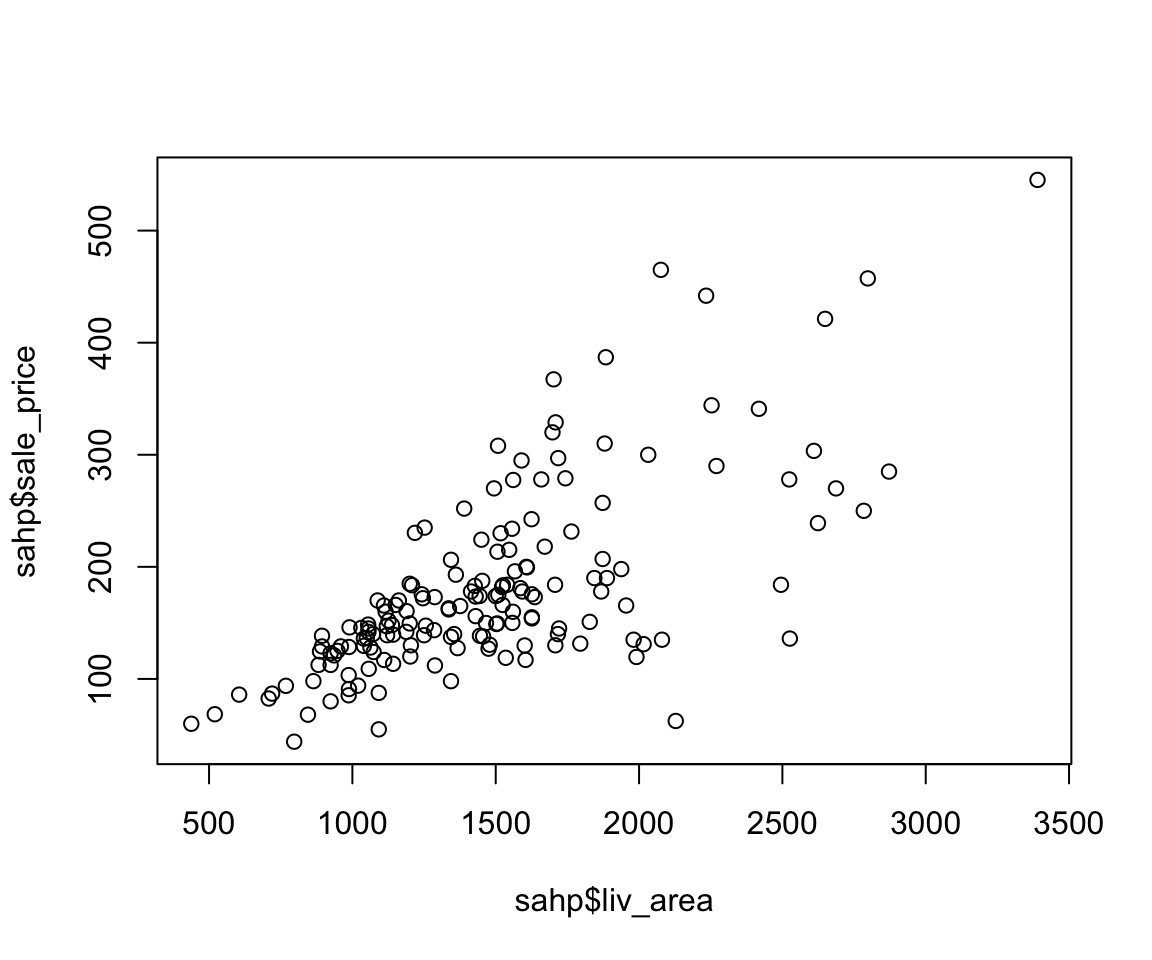
\includegraphics{bookdown-demo_files/figure-latex/unnamed-chunk-140-1.pdf}
From the scatterplot, we can see a clear increasing trend between \texttt{sale\_price} and \texttt{liv\_area}, which is consistent with our intuition. The \texttt{plot()} function provides a rich capability of customization. For example, we can set the labels on the x-axis and y-axis, change the color of the points, etc.

\begin{Shaded}
\begin{Highlighting}[]
\FunctionTok{plot}\NormalTok{(sahp}\SpecialCharTok{$}\NormalTok{liv\_area, sahp}\SpecialCharTok{$}\NormalTok{sale\_price, }\AttributeTok{xlab =} \StringTok{"liv\_area"}\NormalTok{, }\AttributeTok{ylab =} \StringTok{"sale\_price"}\NormalTok{, }\AttributeTok{col =} \StringTok{"red"}\NormalTok{)}
\end{Highlighting}
\end{Shaded}

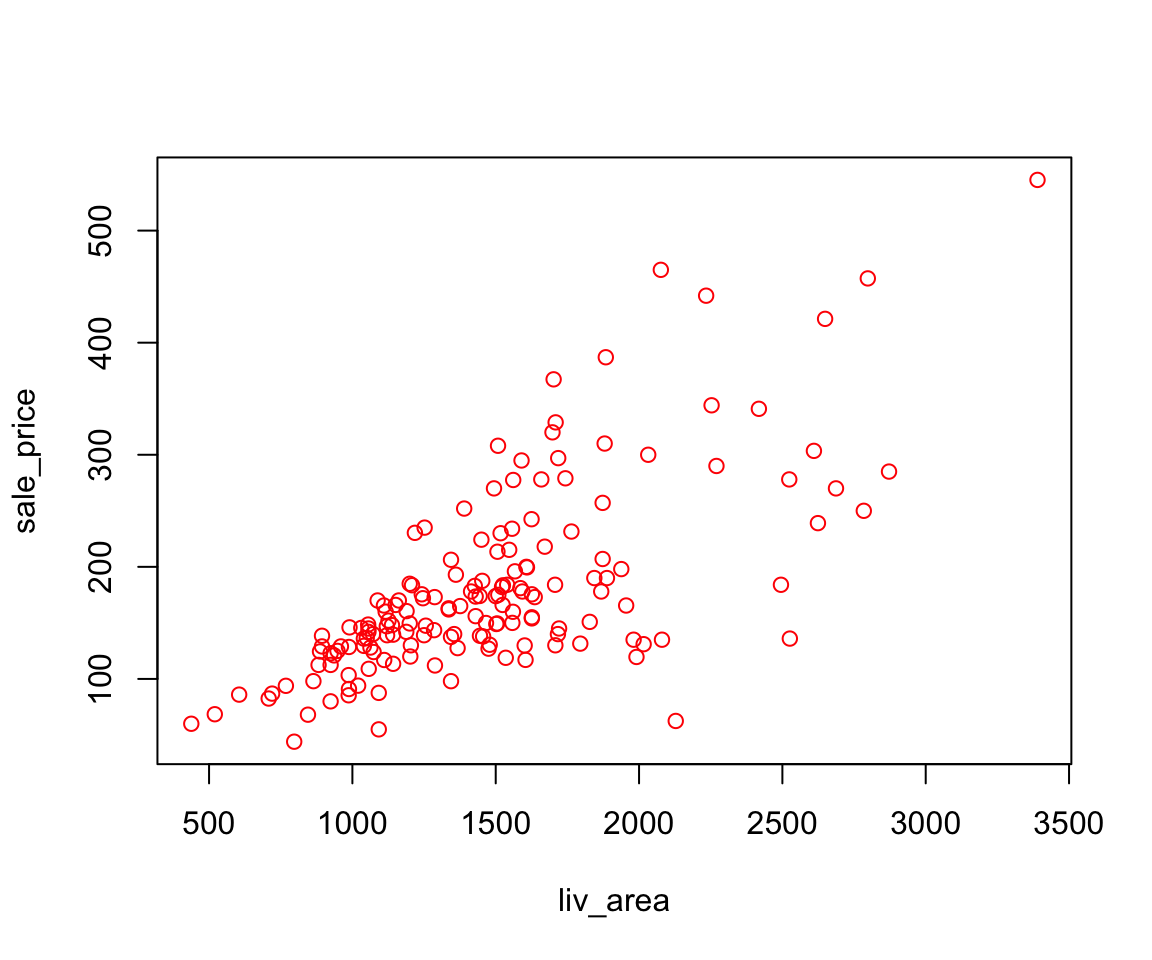
\includegraphics{bookdown-demo_files/figure-latex/unnamed-chunk-141-1.pdf}

\hypertarget{using-the-ggplot-function}{%
\subsection{\texorpdfstring{Using the \texttt{ggplot()} function}{Using the ggplot() function}}\label{using-the-ggplot-function}}

Although the \texttt{plot()} function gets the work done, the \textbf{ggplot2} package provides a superior user experience which allows us to create complex plots with ease. Since the \textbf{ggplot2} package is a member of the \textbf{tidyverse} package, you don't need to install it separately if \textbf{tidyverse} was already installed. Let's first load the package \textbf{ggplot2} and create a scatterplot.

\begin{Shaded}
\begin{Highlighting}[]
\FunctionTok{library}\NormalTok{(ggplot2)}
\FunctionTok{ggplot}\NormalTok{(}\AttributeTok{data =}\NormalTok{ sahp) }\SpecialCharTok{+} \FunctionTok{geom\_point}\NormalTok{(}\AttributeTok{mapping =} \FunctionTok{aes}\NormalTok{(}\AttributeTok{x =}\NormalTok{ liv\_area, }\AttributeTok{y =}\NormalTok{ sale\_price))}
\end{Highlighting}
\end{Shaded}

\begin{verbatim}
#> Warning: Removed 1 rows containing missing values (geom_point).
\end{verbatim}

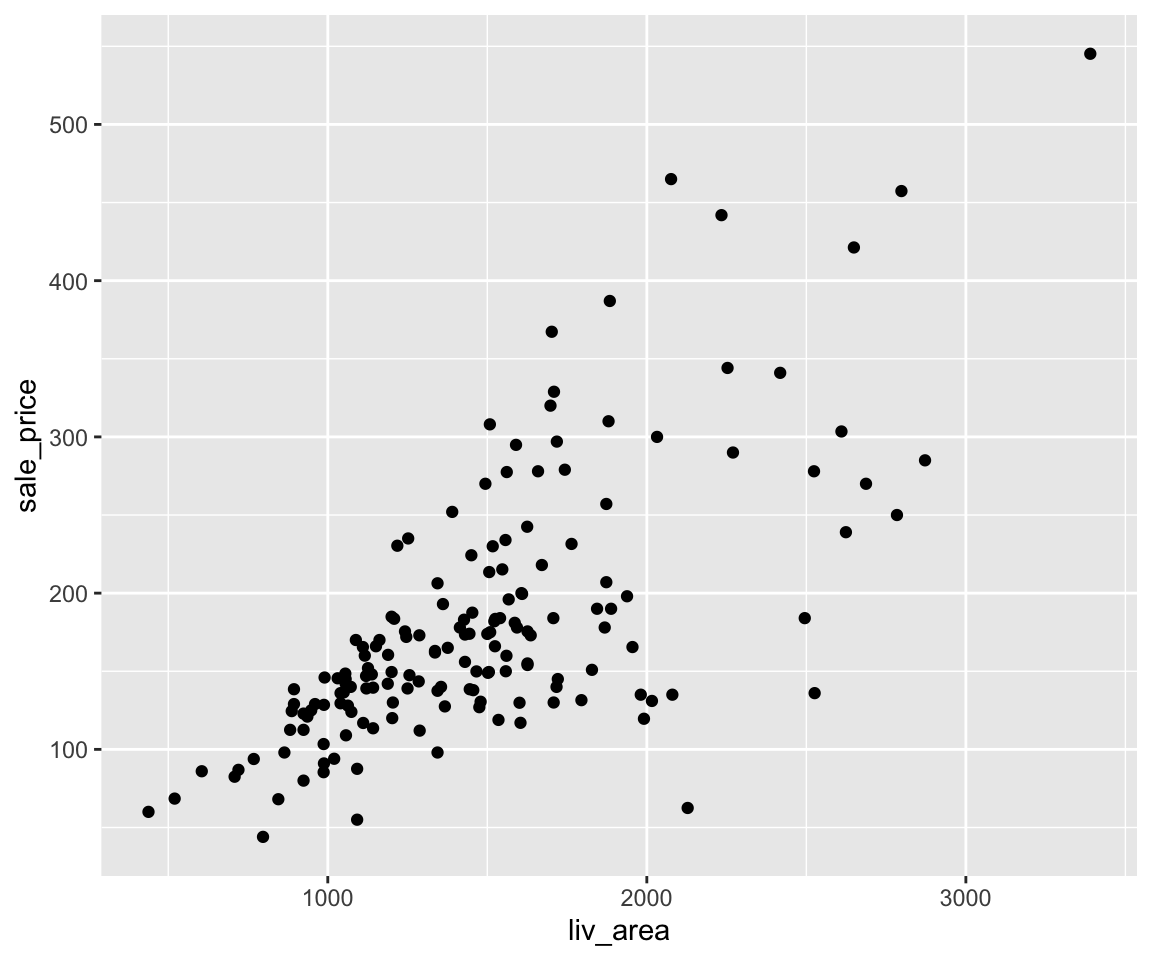
\includegraphics{bookdown-demo_files/figure-latex/unnamed-chunk-142-1.pdf}

Aside from the expected scatterplot, you can see a warning message ``Removed 1 rows containing missing values (geom\_point).'' This indicate that there is 1 row in \texttt{sahp} that contains missing values and it was removed during the plotting process. The removal of missing values is a default behavior for all plots generated by the \textbf{ggplot2} package.

Now, let's walk through the mechanism of \textbf{ggplot2}. In a nutshell, ggplot2 implements the \textbf{grammar of graphics}, a coherent system for describing and building graphs. A more detailed description on the grammar of graphics can be found in \citet{wickham2010layered}.

Let's break it down into two steps. In \textbf{ggplot2}, we always start with the function \texttt{ggplot()} with a data frame or tibble as its argument.

\begin{Shaded}
\begin{Highlighting}[]
\FunctionTok{ggplot}\NormalTok{(}\AttributeTok{data =}\NormalTok{ sahp)}
\end{Highlighting}
\end{Shaded}

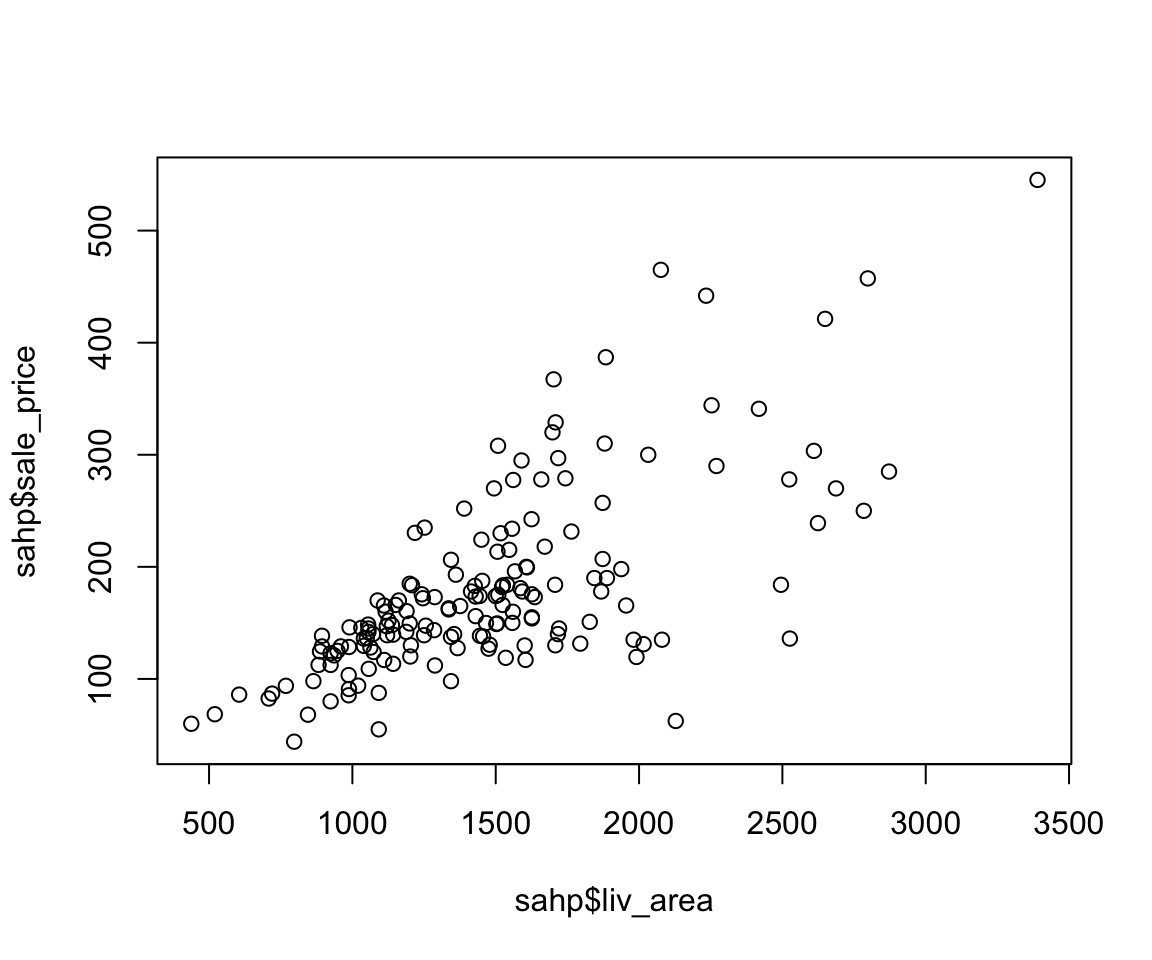
\includegraphics{bookdown-demo_files/figure-latex/unnamed-chunk-143-1.pdf}

After running this code, you can see an empty plot. This is because ggplot does not yet know which variables or what type of plots you want to create. To generate a scatterplot, you can use add a layer using the \texttt{+} operator followed by the \texttt{geom\_point()} function. The \texttt{geom\_point()} is one of the many available geoms in ggplot.

Inside \texttt{geom\_point()}, you need to set the value of the \texttt{mapping} argument. The \texttt{mapping} argument takes a functional form as \texttt{mapping\ =\ aes()}, where the \texttt{aes} is short for aesthetics. For example, you can use \texttt{aes()} to tell ggplot to use which variable on the x-axis, which variable on the y-axis. Let's take another look at this example.

\begin{Shaded}
\begin{Highlighting}[]
\FunctionTok{ggplot}\NormalTok{(}\AttributeTok{data =}\NormalTok{ sahp) }\SpecialCharTok{+} \FunctionTok{geom\_point}\NormalTok{(}\AttributeTok{mapping =} \FunctionTok{aes}\NormalTok{(}\AttributeTok{x =}\NormalTok{ liv\_area, }\AttributeTok{y =}\NormalTok{ sale\_price))}
\end{Highlighting}
\end{Shaded}

Here, inside the \texttt{aes()} function, we set \texttt{x\ =\ liv\_area} and \texttt{y\ =\ sale\_price}, indicating that the variable \texttt{liv\_area} will appear on the x-axis and \texttt{sale\_price} will appear on the y-axis.

\hypertarget{aes}{%
\section{Aesthetics in ggplot}\label{aes}}

Knowing how to generate a scatterplot using \texttt{geom\_point()}, let's discuss one of the most important aspects in a \texttt{geom}, namely, the aesthetics. Aesthetics include various parameters that you can change that affect the appearances of a plot. Some commonly used aesthetics include color, size, shape, and so on.

Note that although we will introduce aesthetics via the example of scatterplot, they are used for all kinds of plots which will be covered at a later time.

\hypertarget{global-aes}{%
\subsection{Global Aesthetics}\label{global-aes}}

First, we discuss \textbf{global aesthetics}, which change certain features of a plot globally.

Let's first review the code we used to generate the scatterplot between \texttt{liv\_area} and \texttt{sale\_price}.

\begin{Shaded}
\begin{Highlighting}[]
\FunctionTok{library}\NormalTok{(ggplot2)}
\FunctionTok{library}\NormalTok{(r02pro)}
\FunctionTok{ggplot}\NormalTok{(}\AttributeTok{data =}\NormalTok{ sahp) }\SpecialCharTok{+} \FunctionTok{geom\_point}\NormalTok{(}\AttributeTok{mapping =} \FunctionTok{aes}\NormalTok{(}\AttributeTok{x =}\NormalTok{ liv\_area, }\AttributeTok{y =}\NormalTok{ sale\_price))}
\end{Highlighting}
\end{Shaded}

\begin{verbatim}
#> Warning: Removed 1 rows containing missing values (geom_point).
\end{verbatim}

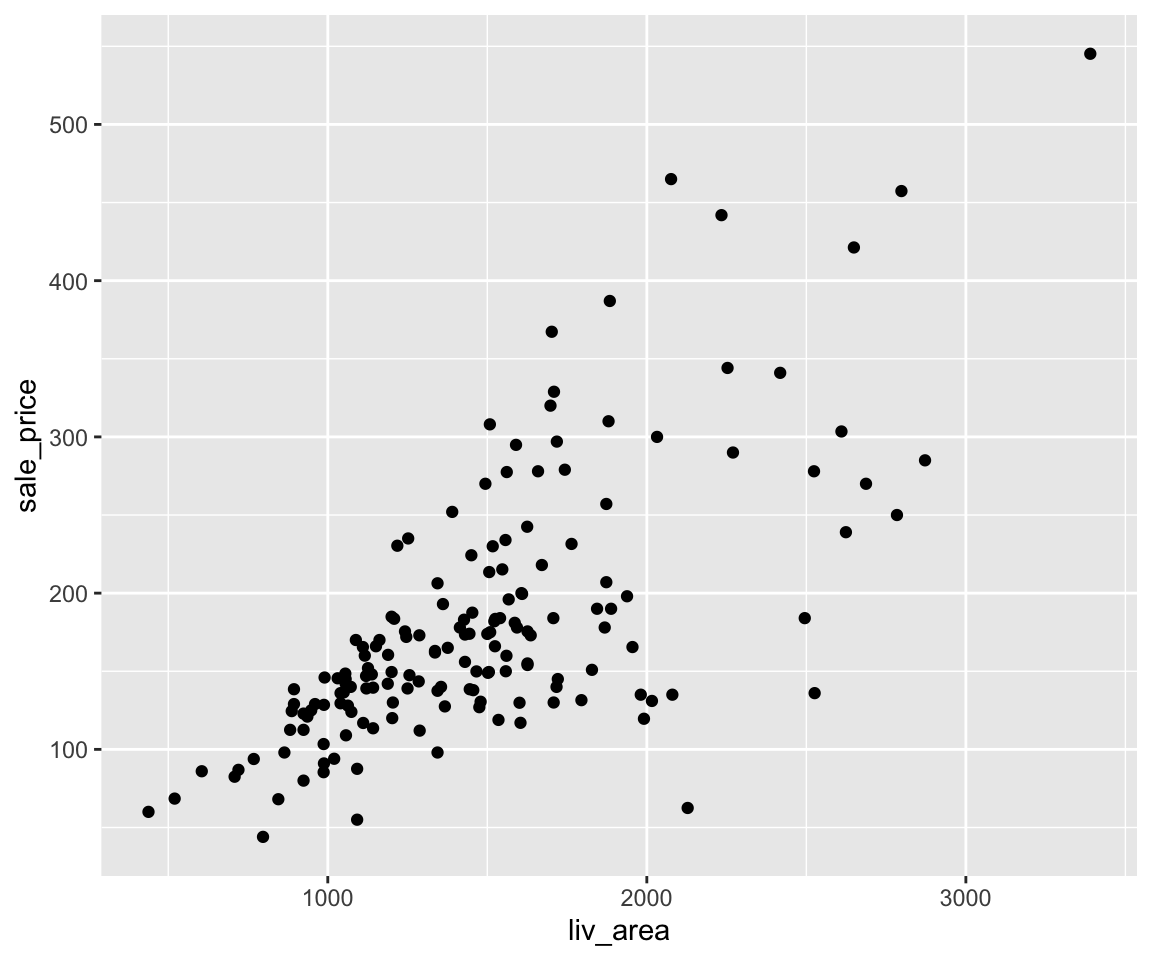
\includegraphics{bookdown-demo_files/figure-latex/unnamed-chunk-145-1.pdf}

Now, let's see how to set \textbf{global aethetics} in \texttt{geom\_point()}.

\textbf{\emph{a. Color}}

To change the color of all points, you can set the \texttt{color} argument in the \texttt{geom\_point()} function. Note that it is placed outside of the \texttt{aes()} function.

\begin{Shaded}
\begin{Highlighting}[]
\FunctionTok{ggplot}\NormalTok{(}\AttributeTok{data =}\NormalTok{ sahp) }\SpecialCharTok{+} \FunctionTok{geom\_point}\NormalTok{(}\AttributeTok{mapping =} \FunctionTok{aes}\NormalTok{(}\AttributeTok{x =}\NormalTok{ liv\_area, }\AttributeTok{y =}\NormalTok{ sale\_price), }\AttributeTok{color =} \StringTok{"red"}\NormalTok{)}
\end{Highlighting}
\end{Shaded}

\begin{verbatim}
#> Warning: Removed 1 rows containing missing values (geom_point).
\end{verbatim}

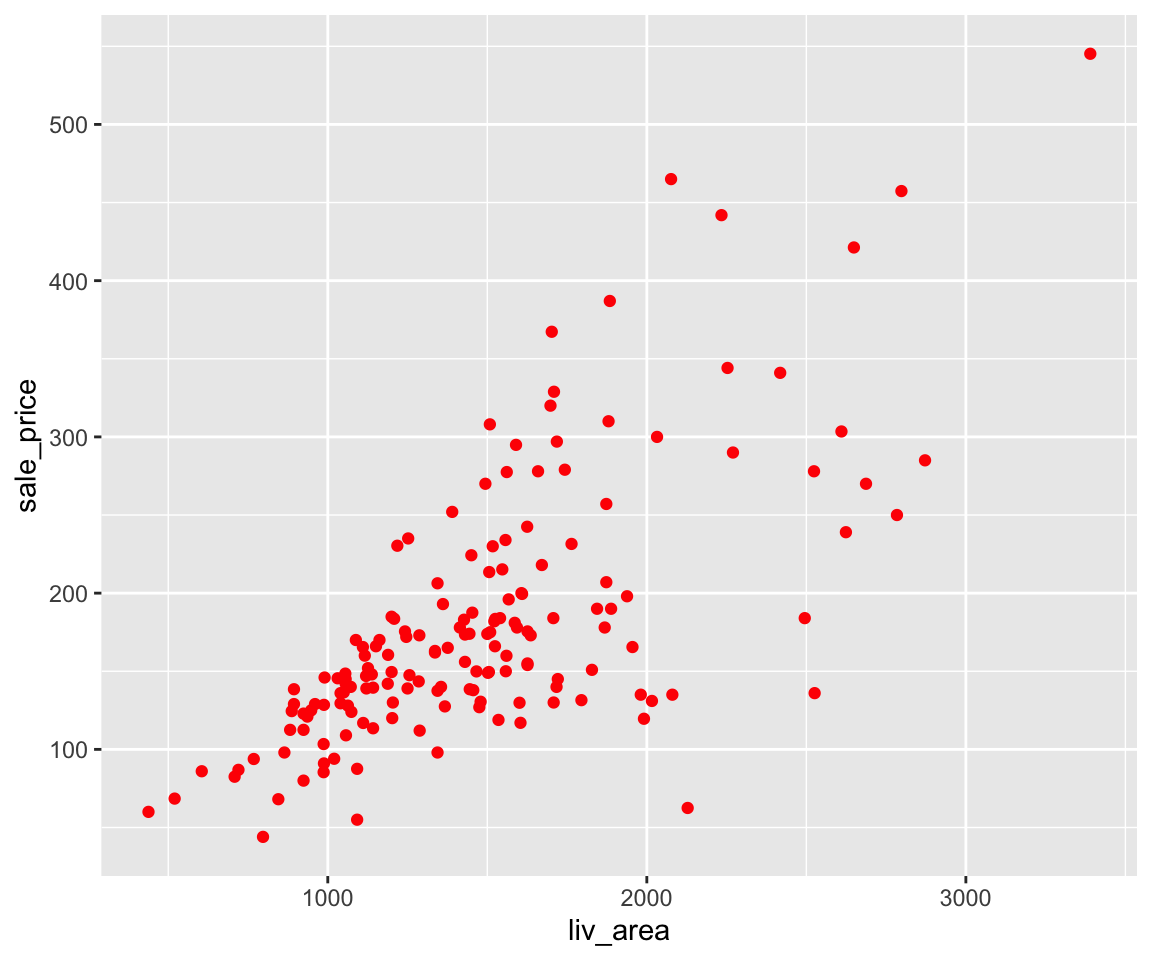
\includegraphics{bookdown-demo_files/figure-latex/unnamed-chunk-146-1.pdf}

Clearly, all points are changed to red.

\textbf{\emph{b. Size}}

Similarly, you can set the \texttt{size} element in the \texttt{geom\_point()} function to change the size of the all points.

\begin{Shaded}
\begin{Highlighting}[]
\FunctionTok{ggplot}\NormalTok{(}\AttributeTok{data =}\NormalTok{ sahp) }\SpecialCharTok{+} \FunctionTok{geom\_point}\NormalTok{(}\AttributeTok{mapping =} \FunctionTok{aes}\NormalTok{(}\AttributeTok{x =}\NormalTok{ liv\_area, }\AttributeTok{y =}\NormalTok{ sale\_price), }\AttributeTok{size =} \DecValTok{3}\NormalTok{)}
\end{Highlighting}
\end{Shaded}

\begin{verbatim}
#> Warning: Removed 1 rows containing missing values (geom_point).
\end{verbatim}

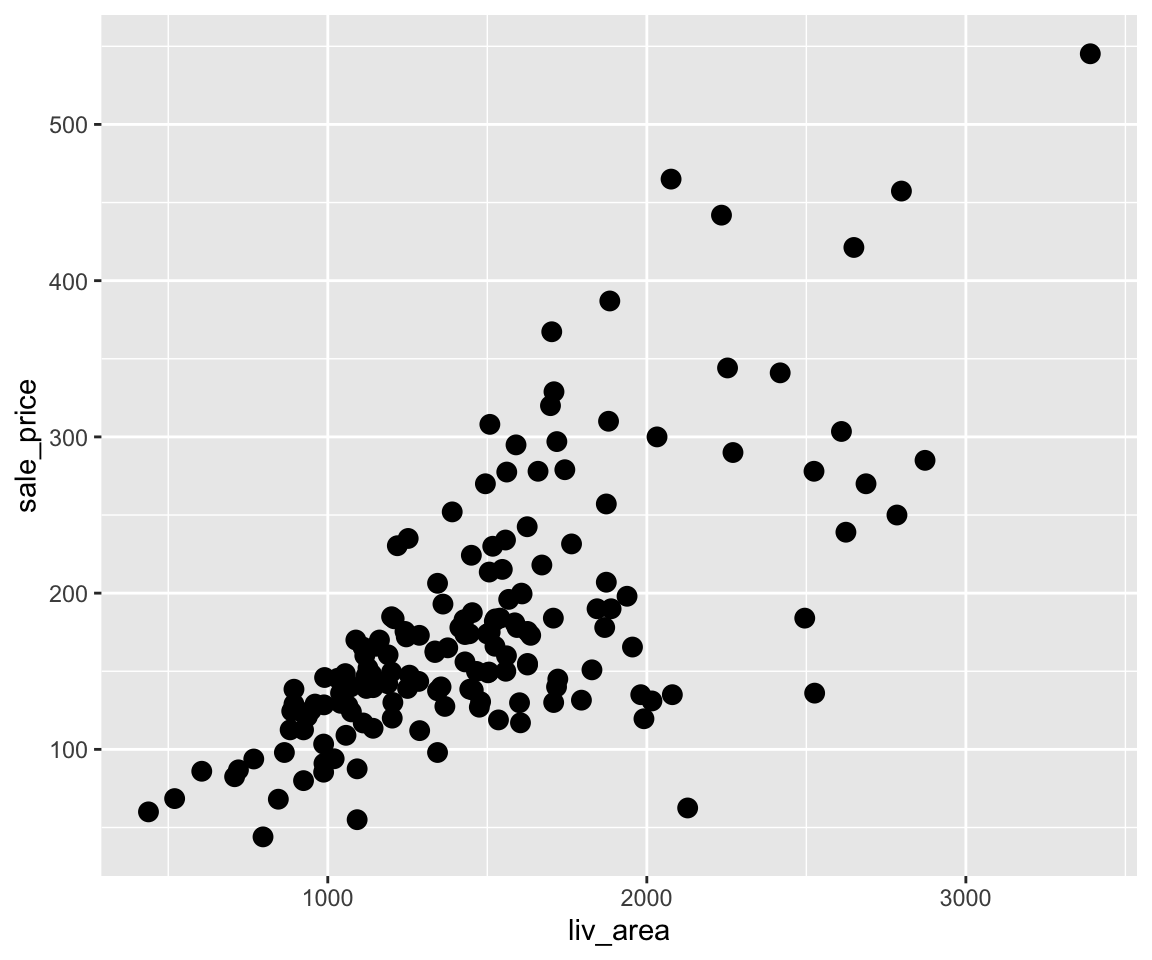
\includegraphics{bookdown-demo_files/figure-latex/unnamed-chunk-147-1.pdf}

You may notice that the points are now bigger than before. Looking at the plot, many points are overlapping with each other, which is sometimes called \textbf{overplotting}. To solve this issue, you can change the transparency level of the points by setting the \texttt{alpha} argument.

\textbf{\emph{c.~Transparency}}

\begin{Shaded}
\begin{Highlighting}[]
\FunctionTok{ggplot}\NormalTok{(}\AttributeTok{data =}\NormalTok{ sahp) }\SpecialCharTok{+} \FunctionTok{geom\_point}\NormalTok{(}\AttributeTok{mapping =} \FunctionTok{aes}\NormalTok{(}\AttributeTok{x =}\NormalTok{ liv\_area, }\AttributeTok{y =}\NormalTok{ sale\_price), }\AttributeTok{size =} \DecValTok{3}\NormalTok{, }\AttributeTok{alpha =} \FloatTok{0.5}\NormalTok{)}
\end{Highlighting}
\end{Shaded}

\begin{verbatim}
#> Warning: Removed 1 rows containing missing values (geom_point).
\end{verbatim}

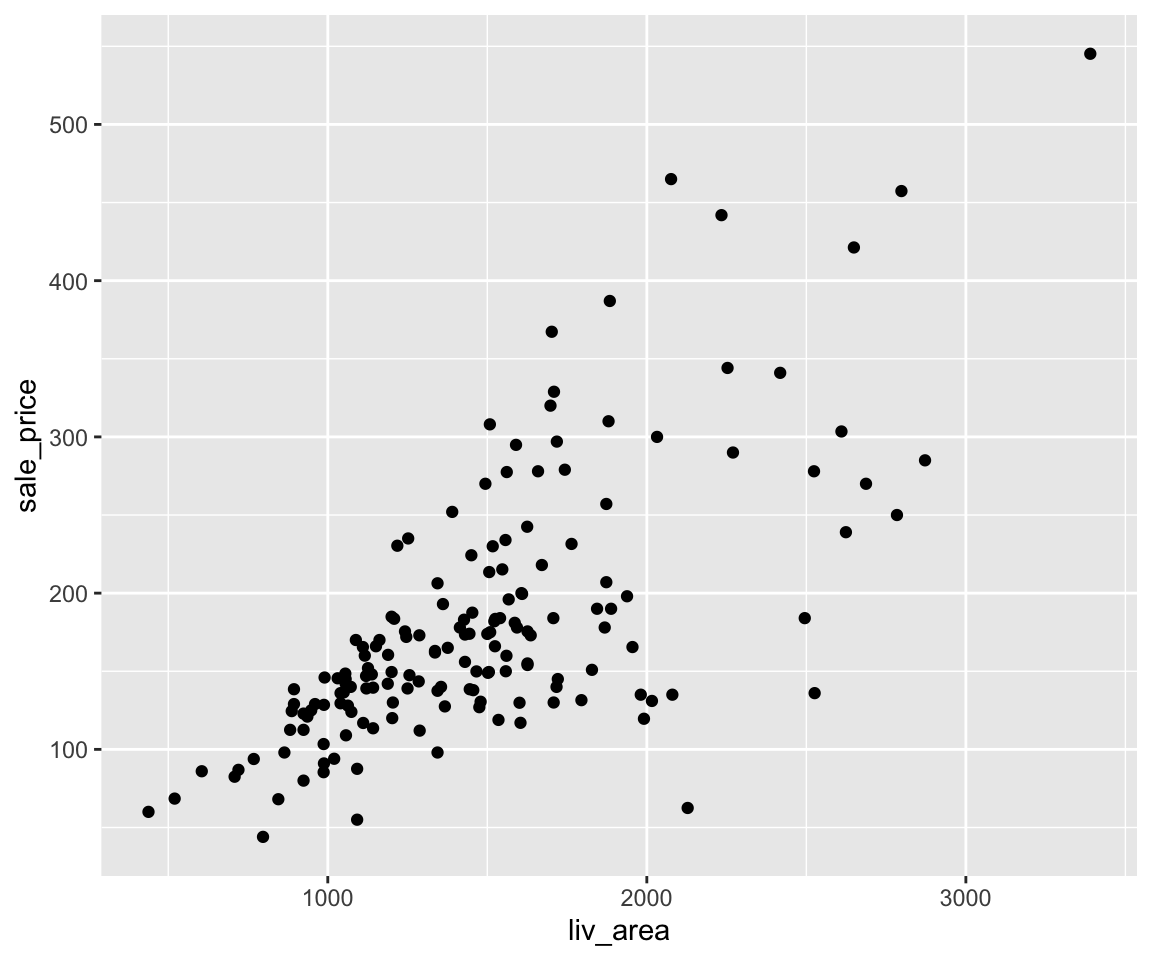
\includegraphics{bookdown-demo_files/figure-latex/unnamed-chunk-148-1.pdf}

By setting \texttt{alpha\ =\ 0.5}, the points become more visible and the overplotting problem is largely alleviated.

\textbf{\emph{d.~Shape}}

Lastly, we can also change the shape of the points from the default one (circle) to other shapes by the \texttt{shape} argument in \texttt{geom\_point()}.

\begin{Shaded}
\begin{Highlighting}[]
\FunctionTok{ggplot}\NormalTok{(}\AttributeTok{data =}\NormalTok{ sahp) }\SpecialCharTok{+} \FunctionTok{geom\_point}\NormalTok{(}\AttributeTok{mapping =} \FunctionTok{aes}\NormalTok{(}\AttributeTok{x =}\NormalTok{ liv\_area, }\AttributeTok{y =}\NormalTok{ sale\_price), }\AttributeTok{shape =} \DecValTok{2}\NormalTok{)}
\end{Highlighting}
\end{Shaded}

\begin{verbatim}
#> Warning: Removed 1 rows containing missing values (geom_point).
\end{verbatim}

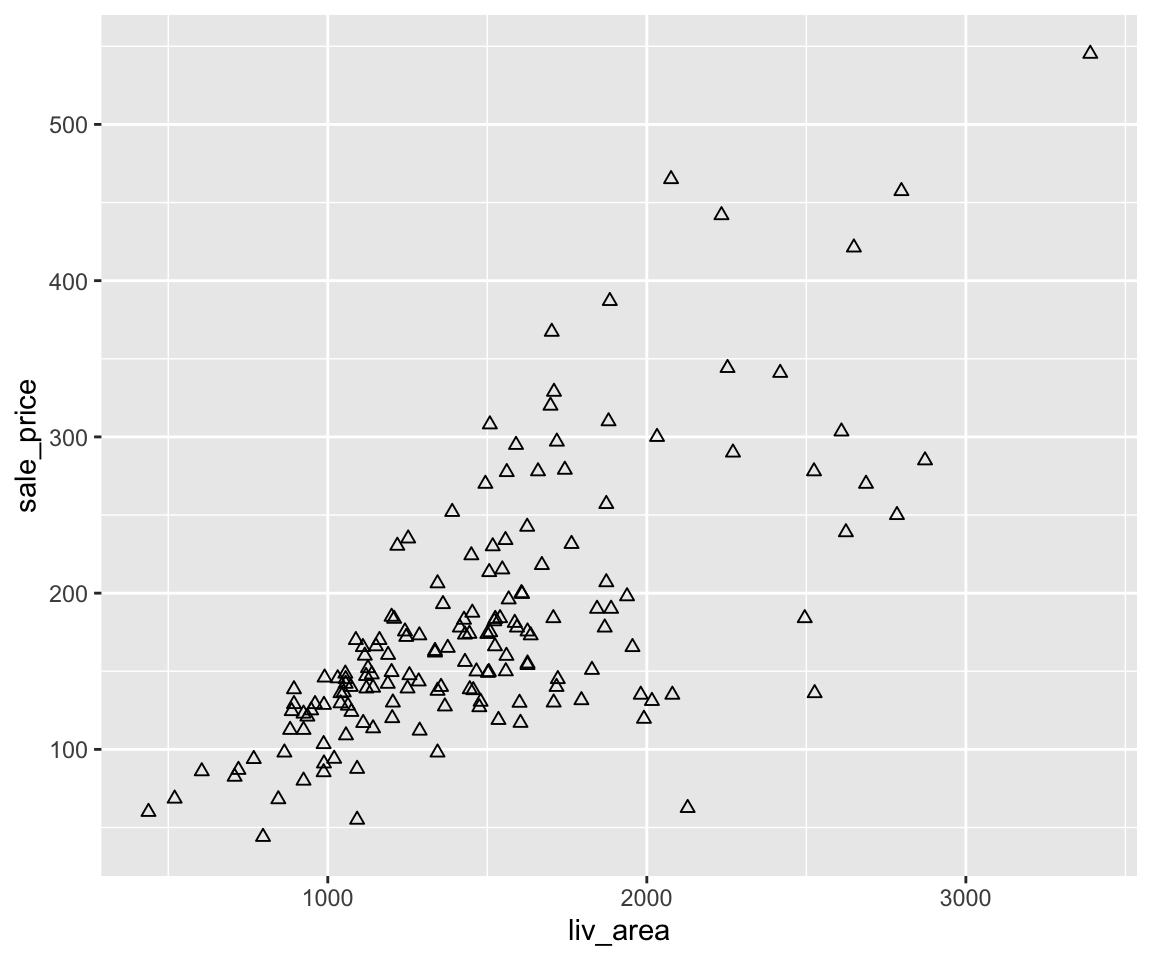
\includegraphics{bookdown-demo_files/figure-latex/unnamed-chunk-149-1.pdf}

\textbf{\emph{e. Multiple Aesthetics}}

Of course, we can combine multiple global aesthetics in the same plot.

\begin{Shaded}
\begin{Highlighting}[]
\FunctionTok{ggplot}\NormalTok{(}\AttributeTok{data =}\NormalTok{ sahp) }\SpecialCharTok{+} \FunctionTok{geom\_point}\NormalTok{(}\AttributeTok{mapping =} \FunctionTok{aes}\NormalTok{(}\AttributeTok{x =}\NormalTok{ liv\_area, }\AttributeTok{y =}\NormalTok{ sale\_price), }\AttributeTok{color =} \StringTok{"red"}\NormalTok{, }\AttributeTok{size =} \DecValTok{3}\NormalTok{, }\AttributeTok{shape =} \DecValTok{2}\NormalTok{)}
\end{Highlighting}
\end{Shaded}

\begin{verbatim}
#> Warning: Removed 1 rows containing missing values (geom_point).
\end{verbatim}

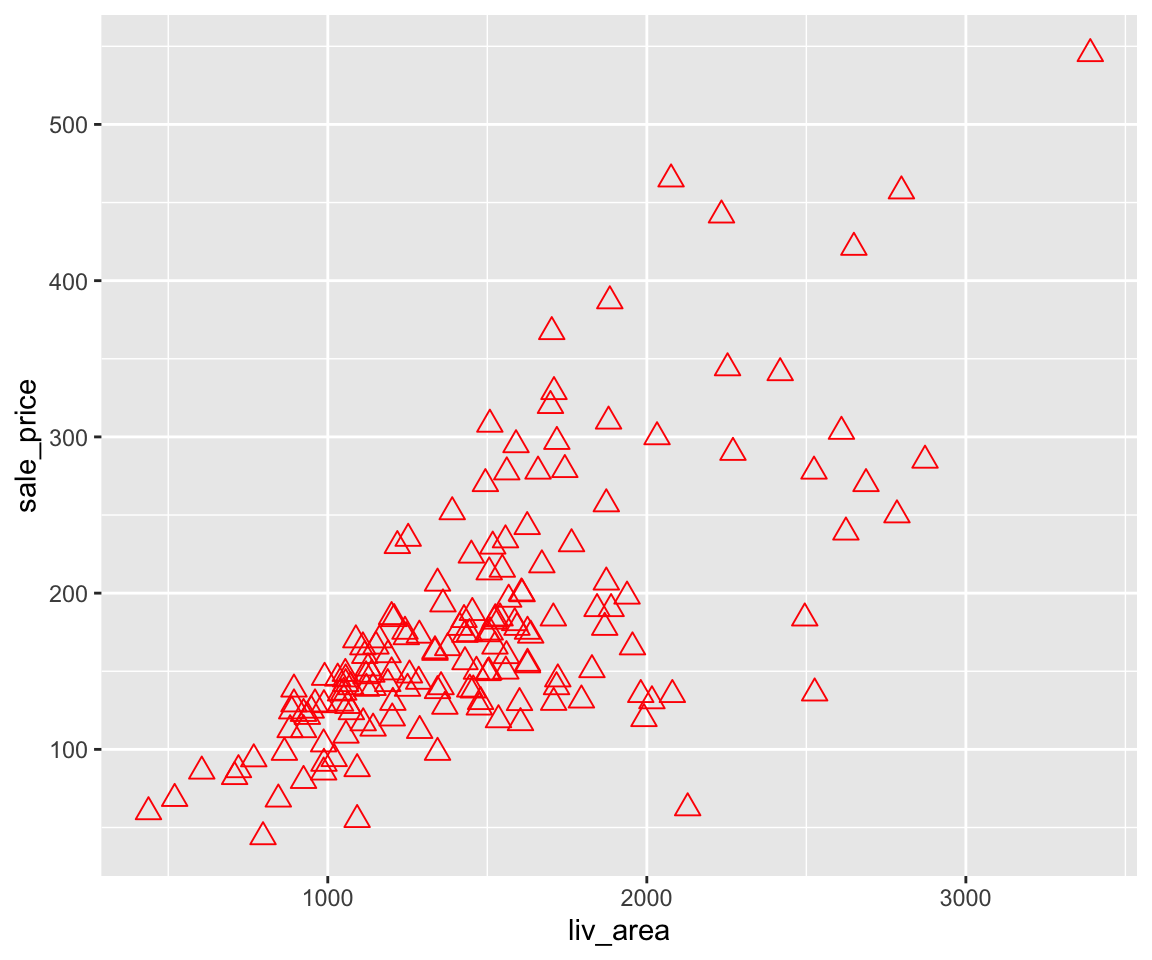
\includegraphics{bookdown-demo_files/figure-latex/unnamed-chunk-150-1.pdf}

Here, we have all points red, size of 3, and of triangle shape.

\hypertarget{map-discrete-aes}{%
\subsection{Map Discrete Variables to Aesthetics}\label{map-discrete-aes}}

Knowing how to use global aesthetics to change the global appearance of a plot, you may want to differentiate different groups with different values of aesthetics. For example, you want to use different colors according to the different \texttt{house\_style} in the scatterplot. To do this, you can map a discrete variable (say \texttt{house\_style}), to an aesthetic (say \texttt{color}) by setting \texttt{color\ =\ house\_style} as an argument in the \texttt{aes()} function.

\textbf{\emph{a. Color}}

Now, let's map \texttt{house\_style} to \texttt{color}.

\begin{Shaded}
\begin{Highlighting}[]
\FunctionTok{ggplot}\NormalTok{(}\AttributeTok{data =}\NormalTok{ sahp) }\SpecialCharTok{+} \FunctionTok{geom\_point}\NormalTok{(}\AttributeTok{mapping =} \FunctionTok{aes}\NormalTok{(}\AttributeTok{x =}\NormalTok{ liv\_area, }\AttributeTok{y =}\NormalTok{ sale\_price, }\AttributeTok{color =}\NormalTok{ house\_style), }\AttributeTok{size =} \DecValTok{3}\NormalTok{)}
\end{Highlighting}
\end{Shaded}

\begin{verbatim}
#> Warning: Removed 1 rows containing missing values (geom_point).
\end{verbatim}

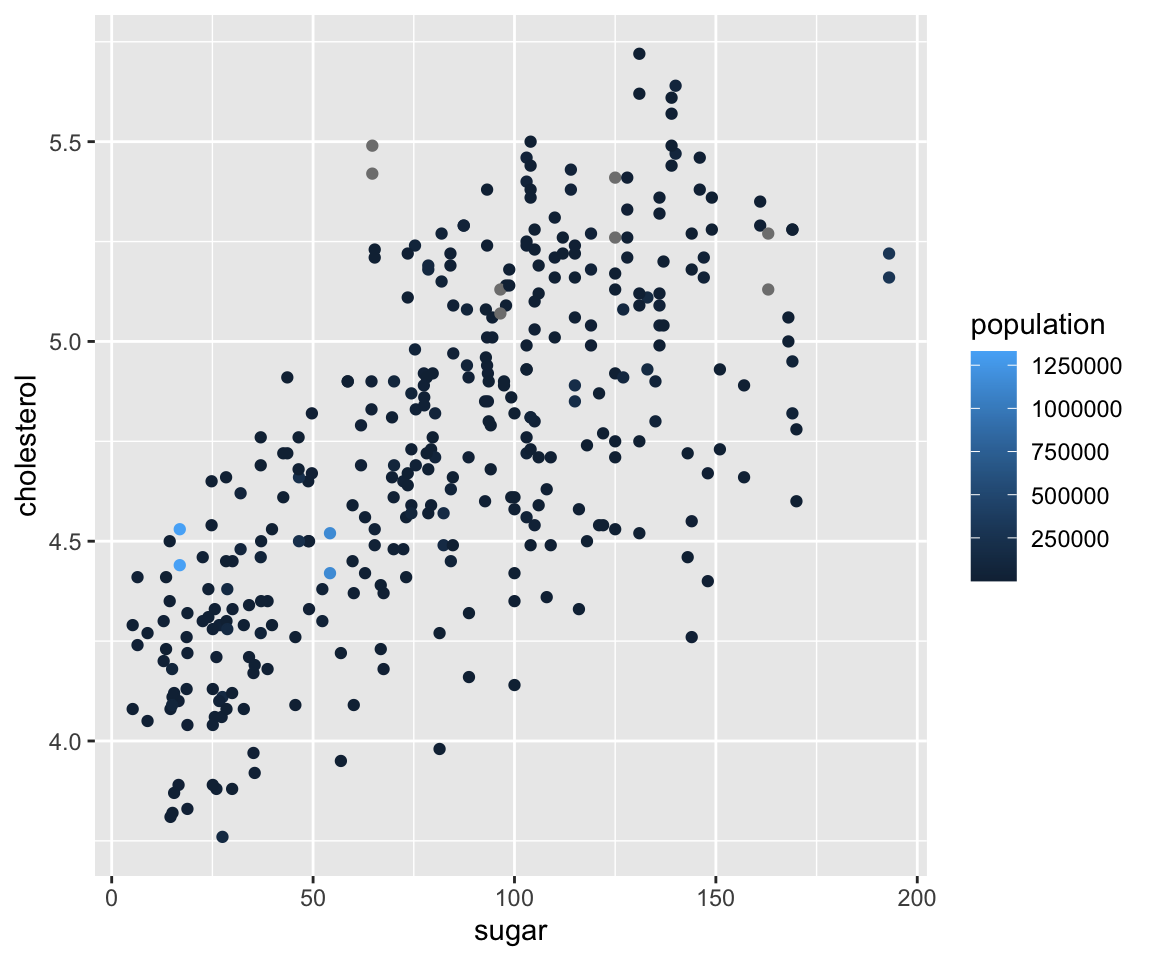
\includegraphics{bookdown-demo_files/figure-latex/scatterplot-color-1.pdf}

From this figure, we can clearly see houses of different styles in distinct colors. In addition, \texttt{ggplot} automatically created a legend to show the correspondence between the house styles and colors.

Sometimes, you may want to use specific colors for different values of the factor. To customize the colors, you can add a layer to the ggplot with function \texttt{scale\_colour\_manual} with argument \texttt{values} containing a character vector consisting of the colors.

\begin{Shaded}
\begin{Highlighting}[]
\FunctionTok{ggplot}\NormalTok{(}\AttributeTok{data =}\NormalTok{ sahp) }\SpecialCharTok{+} \FunctionTok{geom\_point}\NormalTok{(}\AttributeTok{mapping =} \FunctionTok{aes}\NormalTok{(}\AttributeTok{x =}\NormalTok{ liv\_area, }\AttributeTok{y =}\NormalTok{ sale\_price, }\AttributeTok{color =}\NormalTok{ house\_style), }\AttributeTok{size =} \DecValTok{3}\NormalTok{) }\SpecialCharTok{+}  \FunctionTok{scale\_colour\_manual}\NormalTok{(}\AttributeTok{values =} \FunctionTok{c}\NormalTok{(}\StringTok{"red"}\NormalTok{, }\StringTok{"blue"}\NormalTok{, }\StringTok{"green"}\NormalTok{, }\StringTok{"orange"}\NormalTok{,}\StringTok{"purple"}\NormalTok{))}
\end{Highlighting}
\end{Shaded}

\begin{verbatim}
#> Warning: Removed 1 rows containing missing values (geom_point).
\end{verbatim}

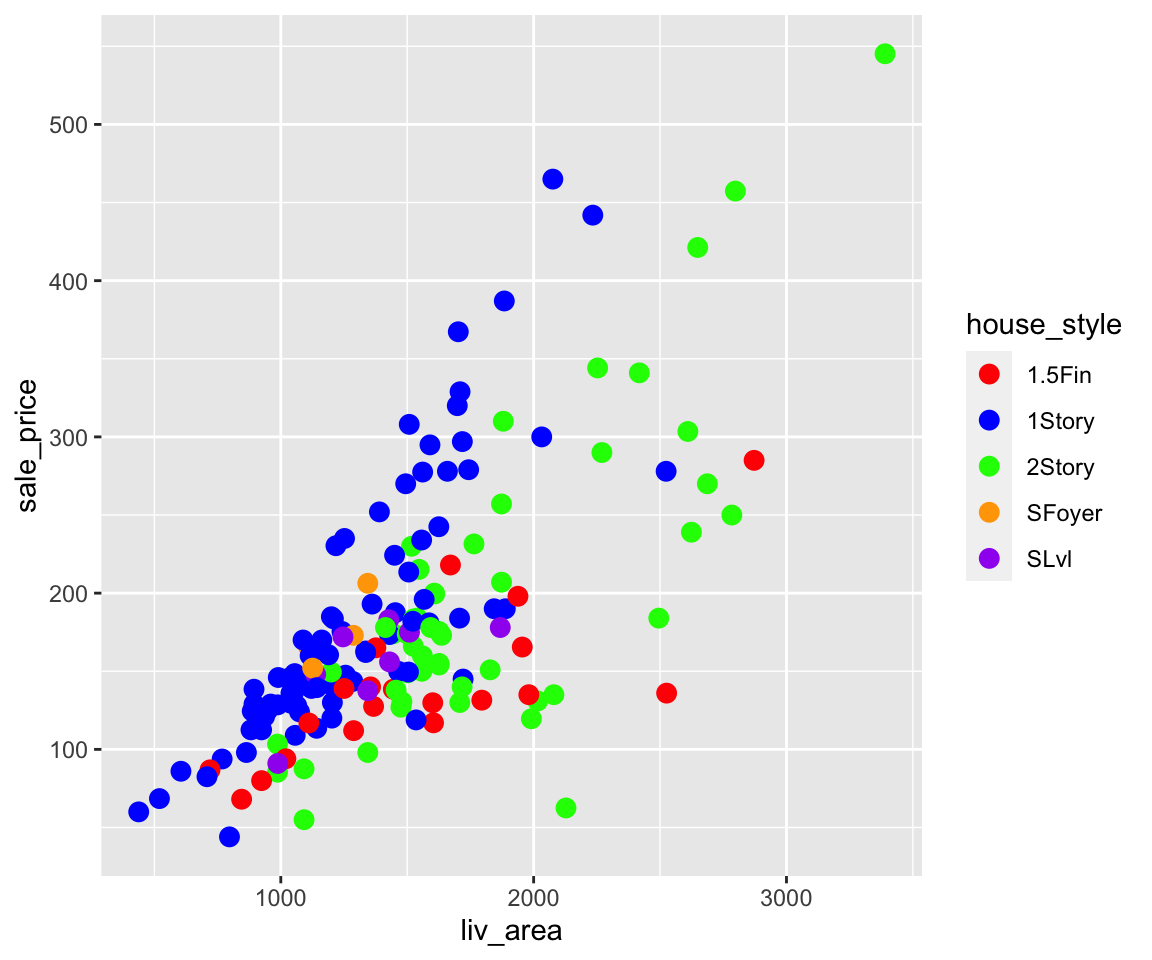
\includegraphics{bookdown-demo_files/figure-latex/unnamed-chunk-151-1.pdf}

Similarly, you can also map \texttt{central\_air} to \texttt{color}.

\begin{Shaded}
\begin{Highlighting}[]
\FunctionTok{ggplot}\NormalTok{(}\AttributeTok{data =}\NormalTok{ sahp) }\SpecialCharTok{+} \FunctionTok{geom\_point}\NormalTok{(}\AttributeTok{mapping =} \FunctionTok{aes}\NormalTok{(}\AttributeTok{x =}\NormalTok{ liv\_area, }\AttributeTok{y =}\NormalTok{ sale\_price, }\AttributeTok{color =}\NormalTok{ central\_air), }\AttributeTok{size =} \DecValTok{3}\NormalTok{)}
\end{Highlighting}
\end{Shaded}

\begin{verbatim}
#> Warning: Removed 1 rows containing missing values (geom_point).
\end{verbatim}

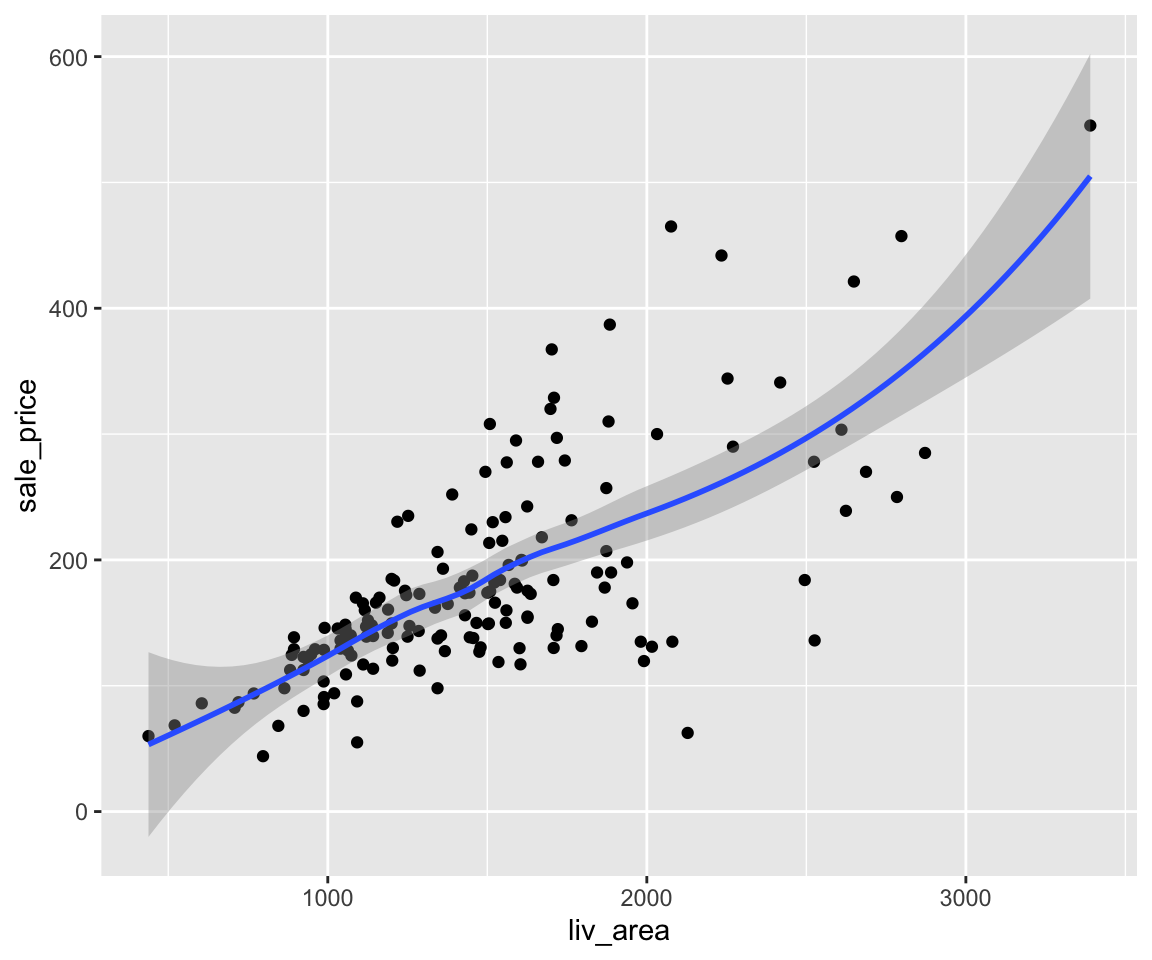
\includegraphics{bookdown-demo_files/figure-latex/unnamed-chunk-152-1.pdf}

The plot tells us the majority of the houses have central AC and the ones without it have relatively lower sale price.

\textbf{\emph{b. Size}}

In addition to color, you can also map a discrete variable to the size aesthetic.

\begin{Shaded}
\begin{Highlighting}[]
\FunctionTok{ggplot}\NormalTok{(}\AttributeTok{data =}\NormalTok{ sahp) }\SpecialCharTok{+} \FunctionTok{geom\_point}\NormalTok{(}\AttributeTok{mapping =} \FunctionTok{aes}\NormalTok{(}\AttributeTok{x =}\NormalTok{ liv\_area, }\AttributeTok{y =}\NormalTok{ sale\_price, }\AttributeTok{size =}\NormalTok{ house\_style), }\AttributeTok{alpha =} \FloatTok{0.5}\NormalTok{)}
\end{Highlighting}
\end{Shaded}

\begin{verbatim}
#> Warning: Using size for a discrete variable is not advised.
\end{verbatim}

\begin{verbatim}
#> Warning: Removed 1 rows containing missing values (geom_point).
\end{verbatim}

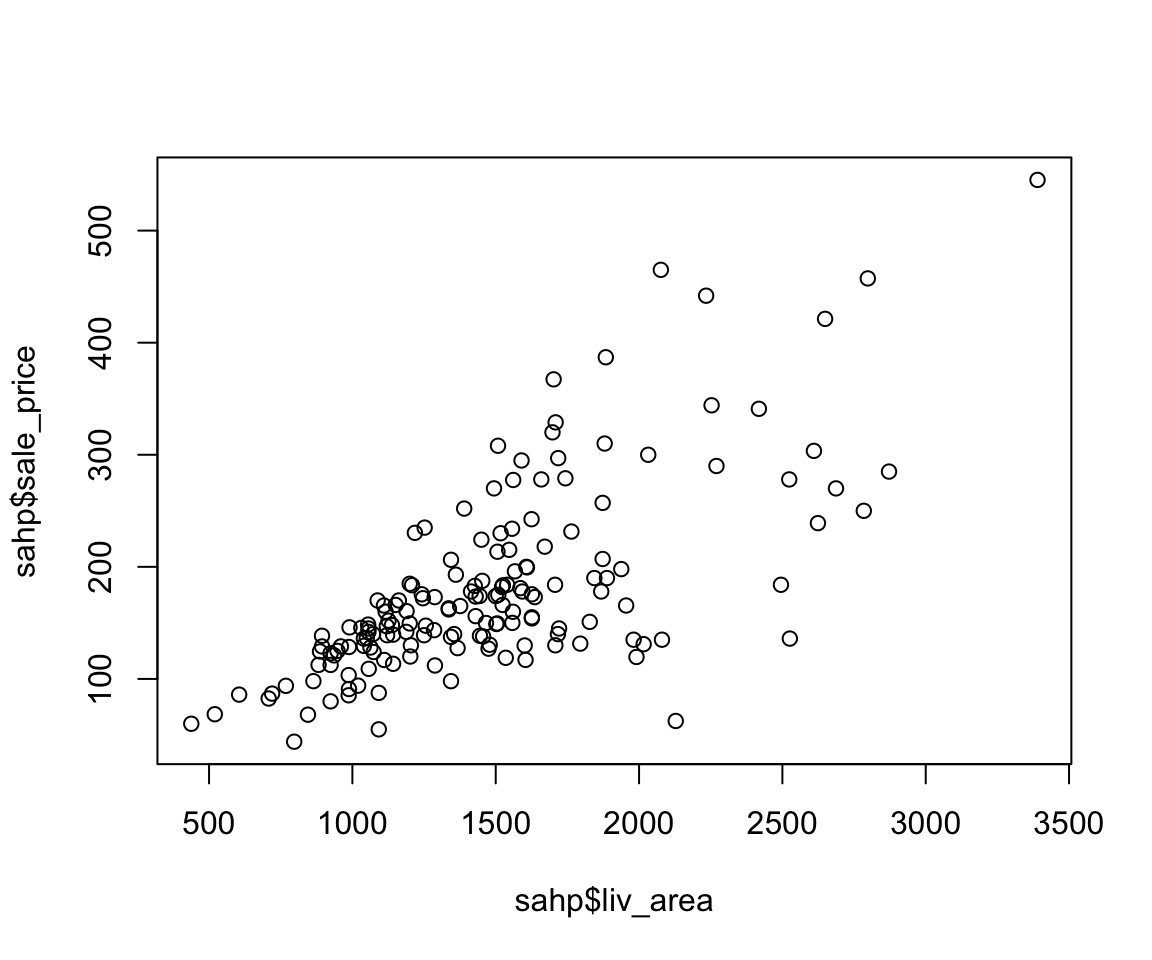
\includegraphics{bookdown-demo_files/figure-latex/unnamed-chunk-153-1.pdf}
You can see from the plot that the sizes of the points are now different according to the \texttt{house\_style}. To alleviate the overplotting issue, we added a global aesthetic \texttt{alpha\ =\ 0.5}, making all points more transparent.

There is a warning message: ``Using size for a discrete variable is not advised.'' The reason is that different sizes may implicitly indicate a particular ordering of the groups, which are usually not clear for a discrete variable.

\textbf{\emph{c.~Shape}}

We can also map a discrete variable to the \texttt{shape} aesthetic.

\begin{Shaded}
\begin{Highlighting}[]
\FunctionTok{ggplot}\NormalTok{(}\AttributeTok{data =}\NormalTok{ sahp) }\SpecialCharTok{+} \FunctionTok{geom\_point}\NormalTok{(}\AttributeTok{mapping =} \FunctionTok{aes}\NormalTok{(}\AttributeTok{x =}\NormalTok{ liv\_area, }\AttributeTok{y =}\NormalTok{ sale\_price, }\AttributeTok{shape =}\NormalTok{ house\_style), }\AttributeTok{size =} \DecValTok{2}\NormalTok{, }\AttributeTok{alpha =} \FloatTok{0.5}\NormalTok{)}
\end{Highlighting}
\end{Shaded}

\begin{verbatim}
#> Warning: Removed 1 rows containing missing values (geom_point).
\end{verbatim}

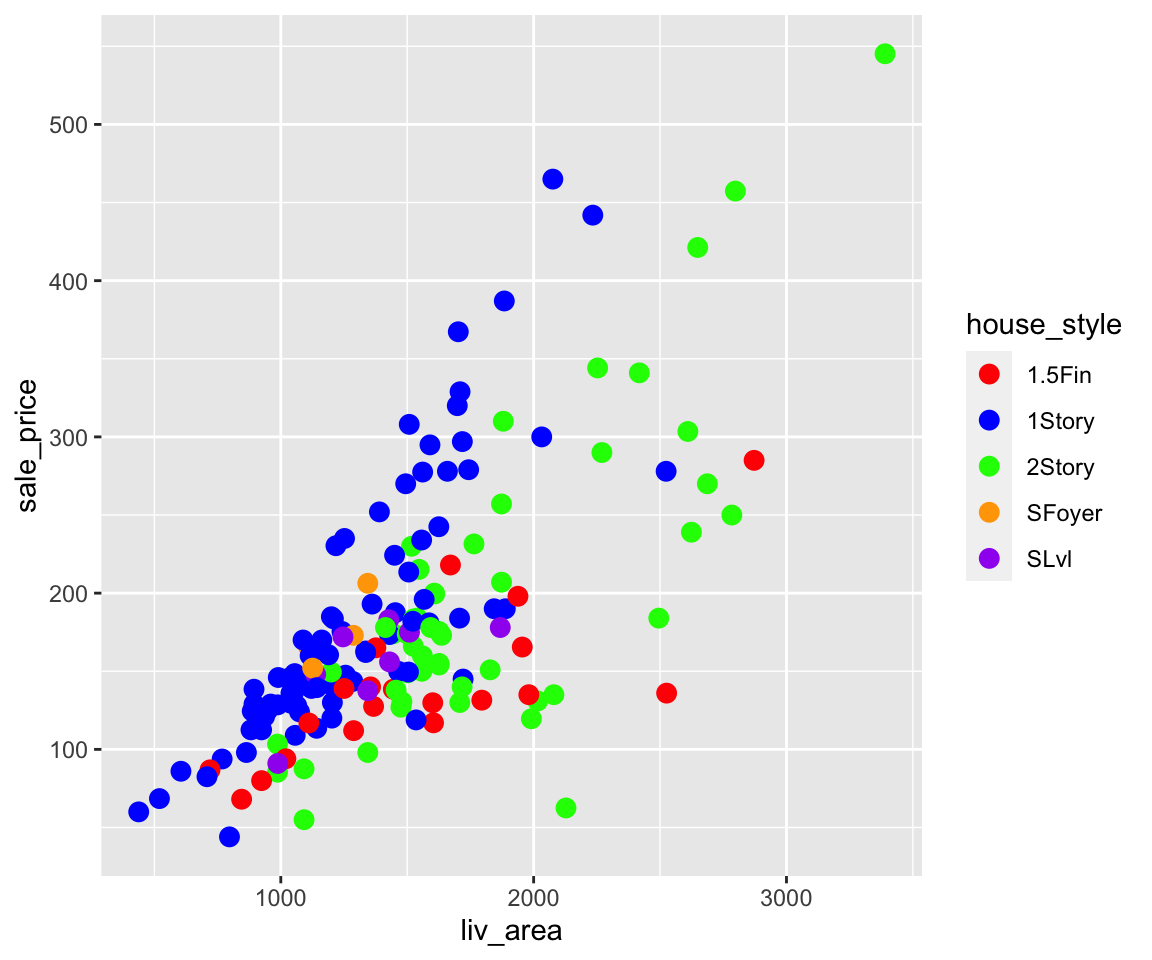
\includegraphics{bookdown-demo_files/figure-latex/unnamed-chunk-154-1.pdf}
Again, we added global aesthetics \texttt{size} and \texttt{alpha} to make the points more visible.

\textbf{\emph{d.~Multiple mappings}}

Just like global aesthetics, you can also have multiple mappings for aesthetics, and mix them with the global aesthetic when necessary.

\begin{Shaded}
\begin{Highlighting}[]
\FunctionTok{ggplot}\NormalTok{(}\AttributeTok{data =}\NormalTok{ sahp) }\SpecialCharTok{+} \FunctionTok{geom\_point}\NormalTok{(}\AttributeTok{mapping =} \FunctionTok{aes}\NormalTok{(}\AttributeTok{x =}\NormalTok{ liv\_area, }\AttributeTok{y =}\NormalTok{ sale\_price, }\AttributeTok{color =}\NormalTok{ house\_style, }\AttributeTok{shape =}\NormalTok{ central\_air), }\AttributeTok{size =} \DecValTok{3}\NormalTok{)}
\end{Highlighting}
\end{Shaded}

\begin{verbatim}
#> Warning: Removed 1 rows containing missing values (geom_point).
\end{verbatim}

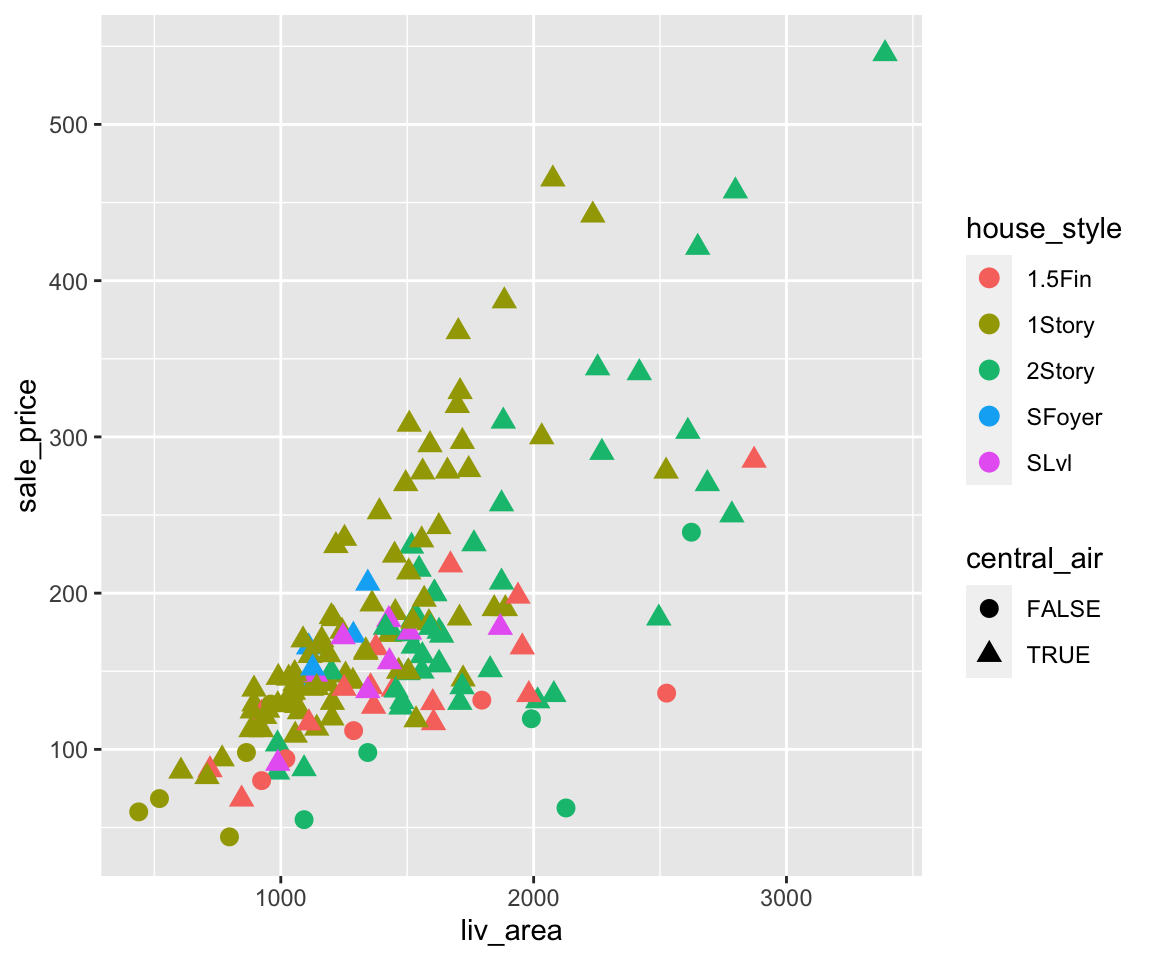
\includegraphics{bookdown-demo_files/figure-latex/unnamed-chunk-155-1.pdf}

Here, we can see the points have different colors according to \texttt{house\_style} and are of different shapes depending on the value of \texttt{central\_air}. Note that there are two legends on the plot showing the color and shape, respectively.

\hypertarget{change-legend-order-via-factors}{%
\subsection{Change Legend Order via Factors}\label{change-legend-order-via-factors}}

Let's first generate a scatterplot between \texttt{liv\_area} and \texttt{sale\_price} where we map the \texttt{heat\_qual} (heating quality) to the \texttt{color} aesthetic.

\begin{Shaded}
\begin{Highlighting}[]
\FunctionTok{ggplot}\NormalTok{(}\AttributeTok{data =}\NormalTok{ sahp) }\SpecialCharTok{+} \FunctionTok{geom\_point}\NormalTok{(}\AttributeTok{mapping =} \FunctionTok{aes}\NormalTok{(}\AttributeTok{x =}\NormalTok{ liv\_area, }\AttributeTok{y =}\NormalTok{ sale\_price, }\AttributeTok{color =}\NormalTok{ heat\_qual), }\AttributeTok{size =} \DecValTok{3}\NormalTok{)}
\end{Highlighting}
\end{Shaded}

\begin{verbatim}
#> Warning: Removed 1 rows containing missing values (geom_point).
\end{verbatim}

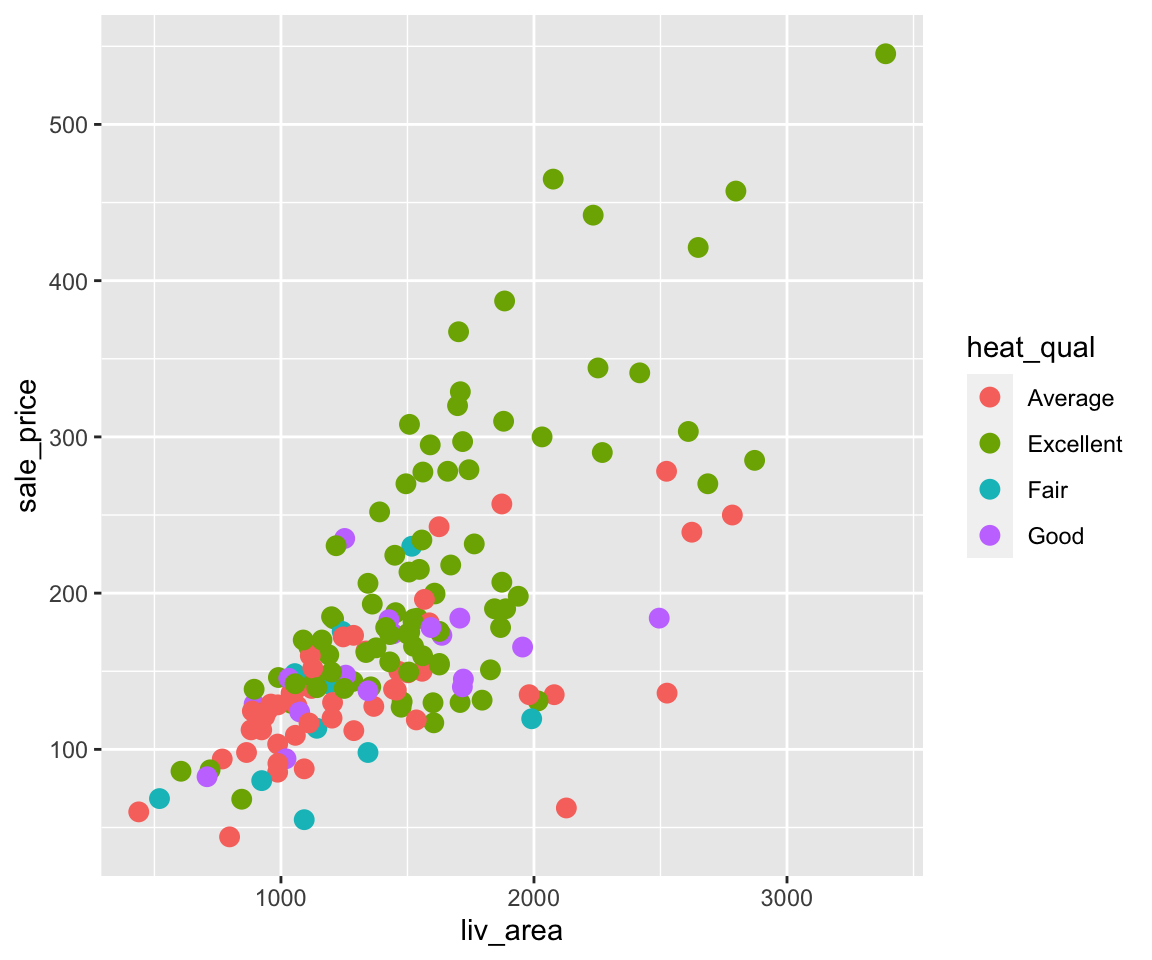
\includegraphics{bookdown-demo_files/figure-latex/unnamed-chunk-156-1.pdf}
Looking at the legend, you can see that different \texttt{heat\_qual} values are in alphabetical order as introduced in Section \ref{sort-vector} when we introduced the ordering of character vectors. Sometimes, you may want to arrange these values in a different order in the plot, for example from the worst to the best. To achieve this, you can use the \texttt{factor()} function with the argument \texttt{levels} which specifies the desired order.

\begin{Shaded}
\begin{Highlighting}[]
\NormalTok{sahp}\SpecialCharTok{$}\NormalTok{heat\_qual }\OtherTok{\textless{}{-}} \FunctionTok{factor}\NormalTok{(sahp}\SpecialCharTok{$}\NormalTok{heat\_qual, }\AttributeTok{levels =} \FunctionTok{c}\NormalTok{(}\StringTok{"Fair"}\NormalTok{,}\StringTok{"Average"}\NormalTok{,}\StringTok{"Good"}\NormalTok{,}\StringTok{"Excellent"}\NormalTok{))}
\FunctionTok{ggplot}\NormalTok{(}\AttributeTok{data =}\NormalTok{ sahp) }\SpecialCharTok{+} \FunctionTok{geom\_point}\NormalTok{(}\AttributeTok{mapping =} \FunctionTok{aes}\NormalTok{(}\AttributeTok{x =}\NormalTok{ liv\_area, }\AttributeTok{y =}\NormalTok{ sale\_price, }\AttributeTok{color =}\NormalTok{ heat\_qual), }\AttributeTok{size =} \DecValTok{3}\NormalTok{)}
\end{Highlighting}
\end{Shaded}

\begin{verbatim}
#> Warning: Removed 1 rows containing missing values (geom_point).
\end{verbatim}

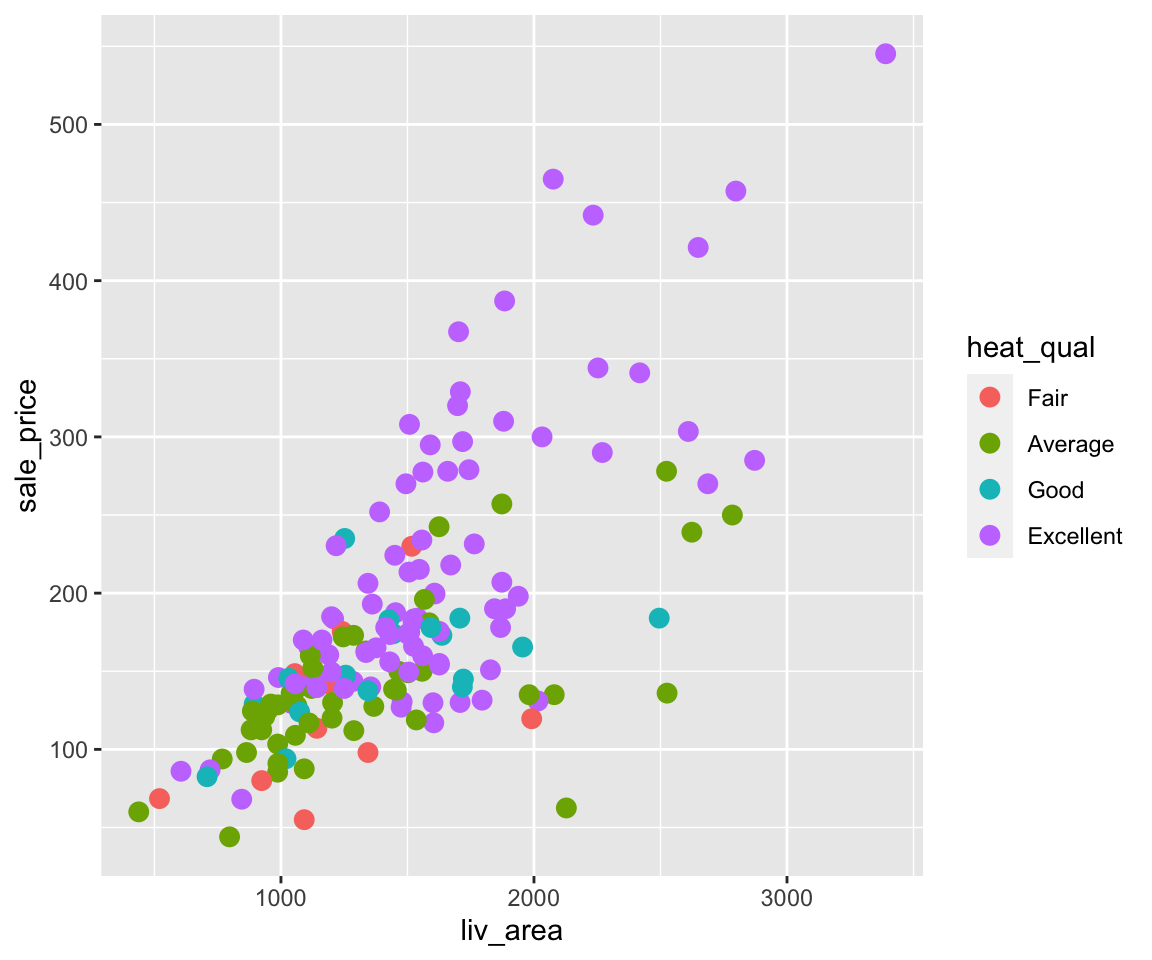
\includegraphics{bookdown-demo_files/figure-latex/unnamed-chunk-157-1.pdf}
After changing the \texttt{heat\_qual} variable to a factor with desired levels, you can see the order in the legend changes accordingly.

\hypertarget{map-continous-aes}{%
\subsection{Map Continuous Variables to Aesthetics}\label{map-continous-aes}}

Knowing how to map discrete variables to aesthetics, it is natural to ask whether we can also map continuous variables to aesthetics. The answer is positive.

\textbf{\emph{a. Color}}
Let's again start with the color aesthetic by mapping \texttt{oa\_qual} to \texttt{color}.

\begin{Shaded}
\begin{Highlighting}[]
\FunctionTok{ggplot}\NormalTok{(}\AttributeTok{data =}\NormalTok{ sahp) }\SpecialCharTok{+} \FunctionTok{geom\_point}\NormalTok{(}\AttributeTok{mapping =} \FunctionTok{aes}\NormalTok{(}\AttributeTok{x =}\NormalTok{ liv\_area, }\AttributeTok{y =}\NormalTok{ sale\_price, }\AttributeTok{color =}\NormalTok{ oa\_qual))}
\end{Highlighting}
\end{Shaded}

\begin{verbatim}
#> Warning: Removed 1 rows containing missing values (geom_point).
\end{verbatim}

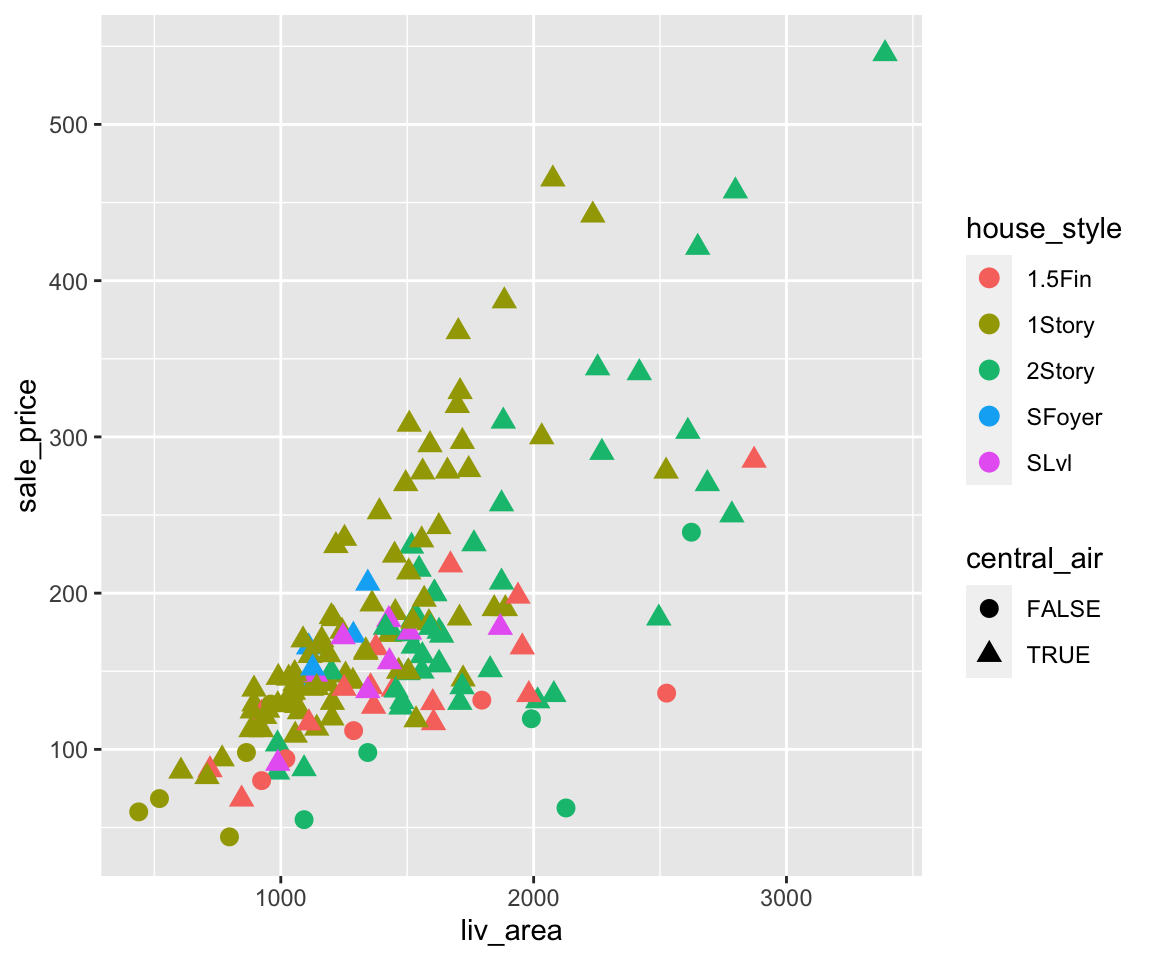
\includegraphics{bookdown-demo_files/figure-latex/unnamed-chunk-158-1.pdf}
Here, we can see the color of all points vary from dark blue to light blue, depending on the value of \texttt{oa\_qual}. Instead of showing different colors in the discrete variable case, the legend now displays a bar showing a continuous color scale according to the value of \texttt{oa\_qual}. To customize the color scale, you can add another lay using the function \texttt{scale\_color\_continuous} with arguments \texttt{low} and \texttt{high} being two colors corresponding to the colors when the variable is of low and high values, respectively.

\begin{Shaded}
\begin{Highlighting}[]
\FunctionTok{ggplot}\NormalTok{(}\AttributeTok{data =}\NormalTok{ sahp) }\SpecialCharTok{+} \FunctionTok{geom\_point}\NormalTok{(}\AttributeTok{mapping =} \FunctionTok{aes}\NormalTok{(}\AttributeTok{x =}\NormalTok{ liv\_area, }\AttributeTok{y =}\NormalTok{ sale\_price, }\AttributeTok{color =}\NormalTok{ oa\_qual)) }\SpecialCharTok{+} \FunctionTok{scale\_color\_continuous}\NormalTok{(}\AttributeTok{low =} \StringTok{"green"}\NormalTok{, }\AttributeTok{high =} \StringTok{"red"}\NormalTok{)}
\end{Highlighting}
\end{Shaded}

\begin{verbatim}
#> Warning: Removed 1 rows containing missing values (geom_point).
\end{verbatim}

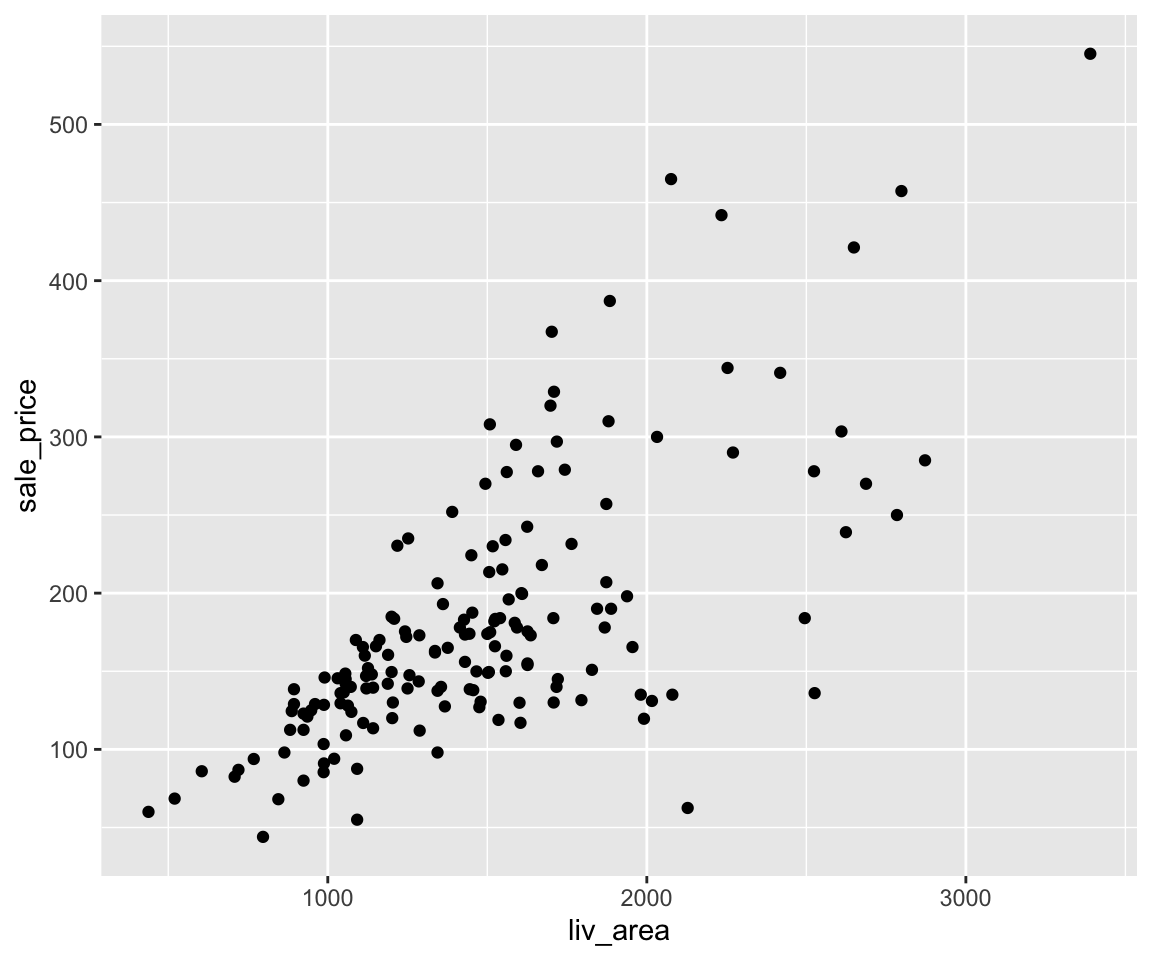
\includegraphics{bookdown-demo_files/figure-latex/unnamed-chunk-159-1.pdf}
Here, the low value of \texttt{oa\_qual} is mapped to green color and the high value of \texttt{oa\_qual} is mapped to red color. You can also try out the following examples.

\begin{Shaded}
\begin{Highlighting}[]
\FunctionTok{ggplot}\NormalTok{(}\AttributeTok{data =}\NormalTok{ sahp) }\SpecialCharTok{+} \FunctionTok{geom\_point}\NormalTok{(}\AttributeTok{mapping =} \FunctionTok{aes}\NormalTok{(}\AttributeTok{x =}\NormalTok{ liv\_area, }\AttributeTok{y =}\NormalTok{ sale\_price, }\AttributeTok{color =}\NormalTok{ oa\_qual)) }\SpecialCharTok{+} \FunctionTok{scale\_color\_continuous}\NormalTok{(}\AttributeTok{low =} \StringTok{"yellow"}\NormalTok{, }\AttributeTok{high =} \StringTok{"blue"}\NormalTok{)}
\end{Highlighting}
\end{Shaded}

\begin{Shaded}
\begin{Highlighting}[]
\FunctionTok{ggplot}\NormalTok{(}\AttributeTok{data =}\NormalTok{ sahp) }\SpecialCharTok{+} \FunctionTok{geom\_point}\NormalTok{(}\AttributeTok{mapping =} \FunctionTok{aes}\NormalTok{(}\AttributeTok{x =}\NormalTok{ liv\_area, }\AttributeTok{y =}\NormalTok{ sale\_price, }\AttributeTok{color =}\NormalTok{ bedroom), }\AttributeTok{size =} \DecValTok{3}\NormalTok{) }\SpecialCharTok{+} \FunctionTok{scale\_color\_continuous}\NormalTok{(}\AttributeTok{low =} \StringTok{"yellow"}\NormalTok{, }\AttributeTok{high =} \StringTok{"blue"}\NormalTok{)}
\end{Highlighting}
\end{Shaded}

\textbf{\emph{b. Size}}

In addition to the color aesthetic, we can also map continuous variables to the size aesthetic.

\begin{Shaded}
\begin{Highlighting}[]
\FunctionTok{ggplot}\NormalTok{(}\AttributeTok{data =}\NormalTok{ sahp) }\SpecialCharTok{+} \FunctionTok{geom\_point}\NormalTok{(}\AttributeTok{mapping =} \FunctionTok{aes}\NormalTok{(}\AttributeTok{x =}\NormalTok{ liv\_area, }\AttributeTok{y =}\NormalTok{ sale\_price, }\AttributeTok{size =}\NormalTok{ lot\_area))}
\end{Highlighting}
\end{Shaded}

\begin{verbatim}
#> Warning: Removed 1 rows containing missing values (geom_point).
\end{verbatim}

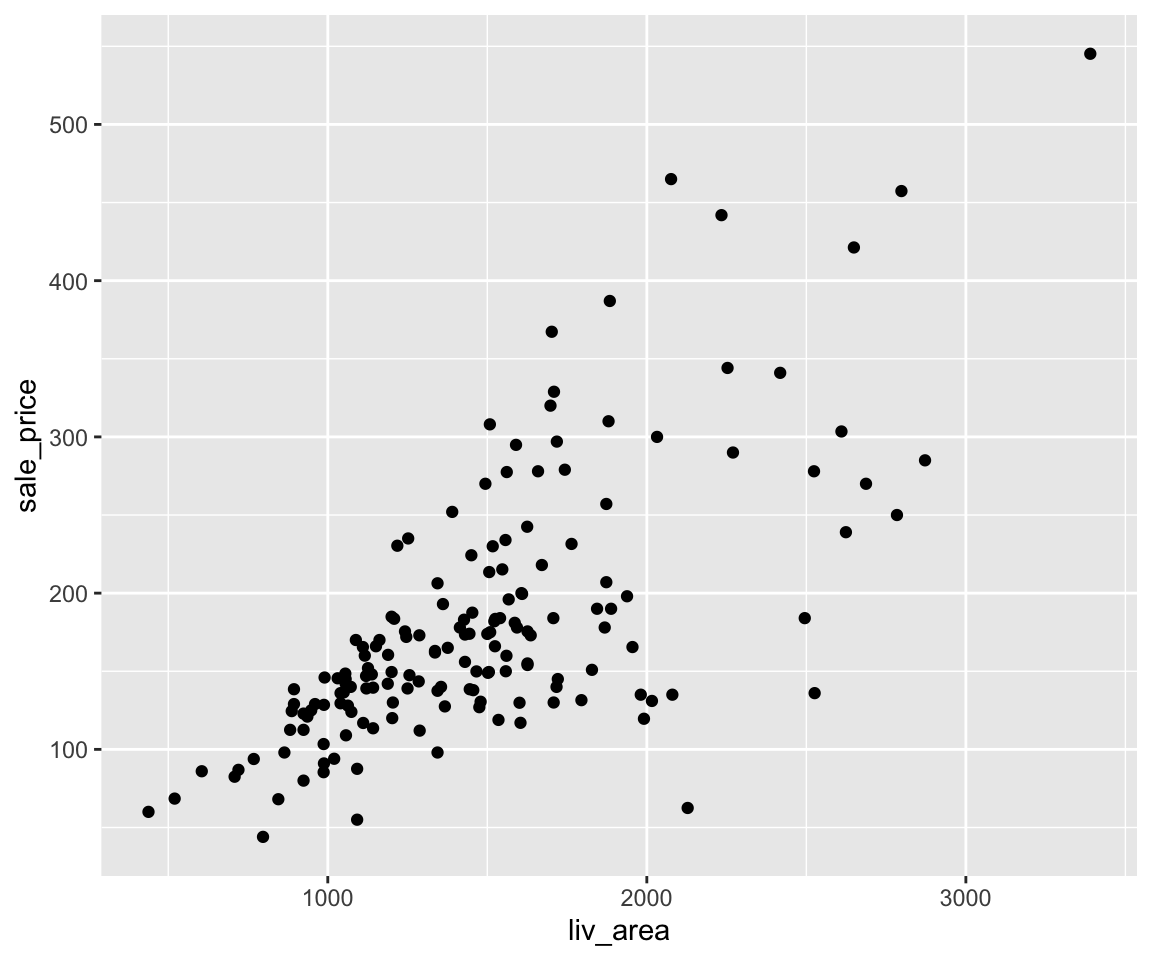
\includegraphics{bookdown-demo_files/figure-latex/unnamed-chunk-162-1.pdf}
In this example, you can see the points corresponding to larger \texttt{lot\_area} values are larger than those corresponding to smaller \texttt{lot\_area} values. Note that although the legend only shows three different sizes, the actual size of the point is continuous corresponding to the value of \texttt{lot\_area}.

How about the shape aesthetic? Can we map a continuous variable to it? Let's try it.

\begin{Shaded}
\begin{Highlighting}[]
\FunctionTok{ggplot}\NormalTok{(}\AttributeTok{data =}\NormalTok{ sahp) }\SpecialCharTok{+} \FunctionTok{geom\_point}\NormalTok{(}\AttributeTok{mapping =} \FunctionTok{aes}\NormalTok{(}\AttributeTok{x =}\NormalTok{ liv\_area, }\AttributeTok{y =}\NormalTok{ sale\_price, }\AttributeTok{shape =}\NormalTok{ lot\_area)) }\CommentTok{\#continuous variable can not be mapped to shape}
\end{Highlighting}
\end{Shaded}

\begin{verbatim}
#> Error: A continuous variable can not be mapped to shape
\end{verbatim}


\includegraphics{bookdown-demo_files/figure-latex/unnamed-chunk-163-1.pdf}
You see an error message: ``A continuous variable can not be mapped to shape''. The reason is intuitive: the shape can't be naturally changed continuously.

\hypertarget{map-converted-logical-variable-to-aesthetics}{%
\subsection{Map Converted Logical Variable to Aesthetics}\label{map-converted-logical-variable-to-aesthetics}}

Lastly, you can also create logical variables on the fly and map them to aesthetics. For example, if you want to differentiate the points according to whether the value of \texttt{lot\_area} is larger than 1e4, a logical variable \texttt{lot\_area\ \textgreater{}\ 1e4} can be created.

\begin{Shaded}
\begin{Highlighting}[]
\FunctionTok{ggplot}\NormalTok{(}\AttributeTok{data =}\NormalTok{ sahp) }\SpecialCharTok{+} \FunctionTok{geom\_point}\NormalTok{(}\AttributeTok{mapping =} \FunctionTok{aes}\NormalTok{(}\AttributeTok{x =}\NormalTok{ liv\_area, }\AttributeTok{y =}\NormalTok{ sale\_price, }\AttributeTok{shape =}\NormalTok{ lot\_area }\SpecialCharTok{\textgreater{}} \FloatTok{1e4}\NormalTok{), }\AttributeTok{size =} \DecValTok{3}\NormalTok{)}
\end{Highlighting}
\end{Shaded}

\begin{verbatim}
#> Warning: Removed 1 rows containing missing values (geom_point).
\end{verbatim}

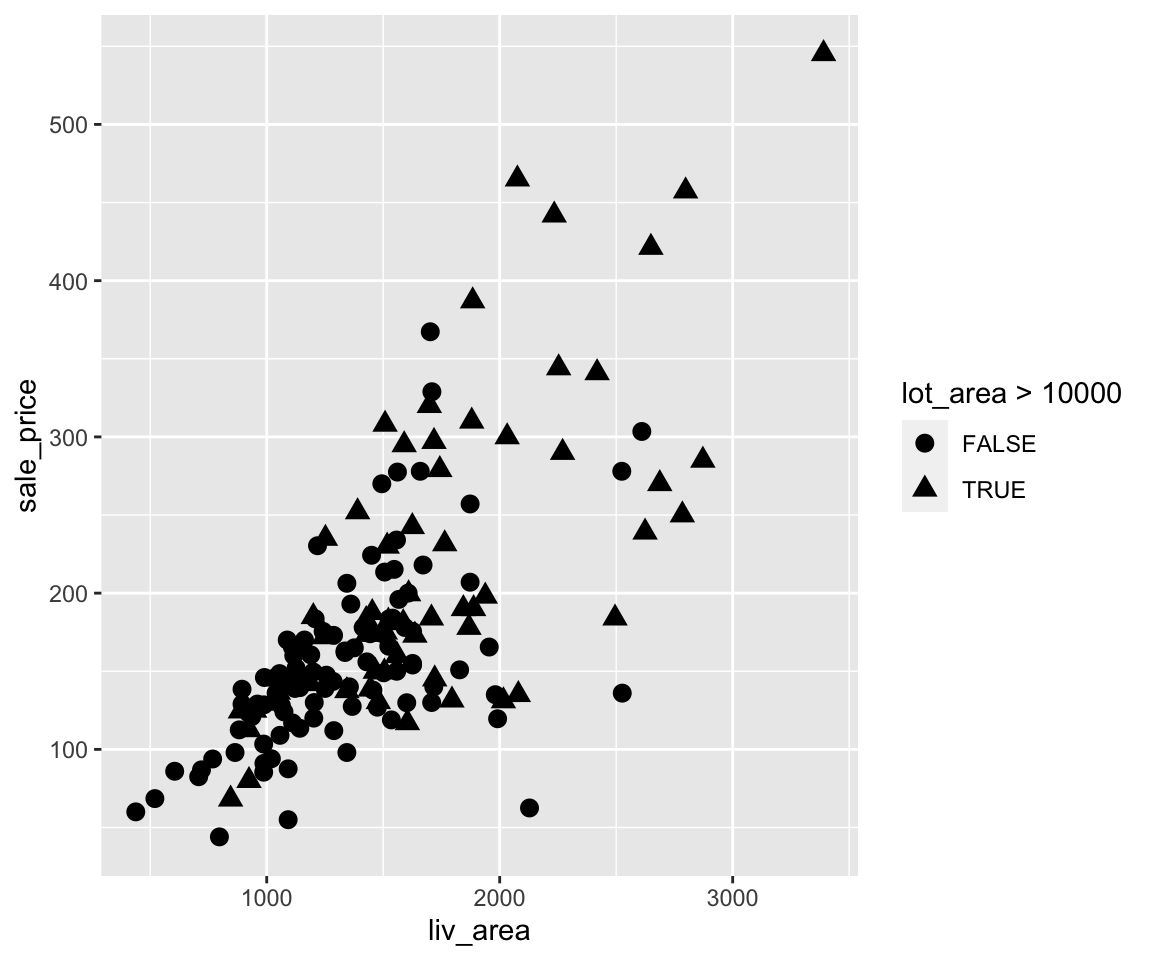
\includegraphics{bookdown-demo_files/figure-latex/unnamed-chunk-164-1.pdf}

We can see the houses with \texttt{lot\_area} larger than 1e4 are of different color from those with less than 1e4 in lot area.

Let's see another example where we want to highlight the different between two-story houses from the other types.

\begin{Shaded}
\begin{Highlighting}[]
\FunctionTok{ggplot}\NormalTok{(}\AttributeTok{data =}\NormalTok{ sahp) }\SpecialCharTok{+} \FunctionTok{geom\_point}\NormalTok{(}\AttributeTok{mapping =} \FunctionTok{aes}\NormalTok{(}\AttributeTok{x =}\NormalTok{ liv\_area, }\AttributeTok{y =}\NormalTok{ sale\_price, }\AttributeTok{shape =}\NormalTok{ house\_style }\SpecialCharTok{==} \StringTok{"2Story"}\NormalTok{))}
\end{Highlighting}
\end{Shaded}

\begin{verbatim}
#> Warning: Removed 1 rows containing missing values (geom_point).
\end{verbatim}

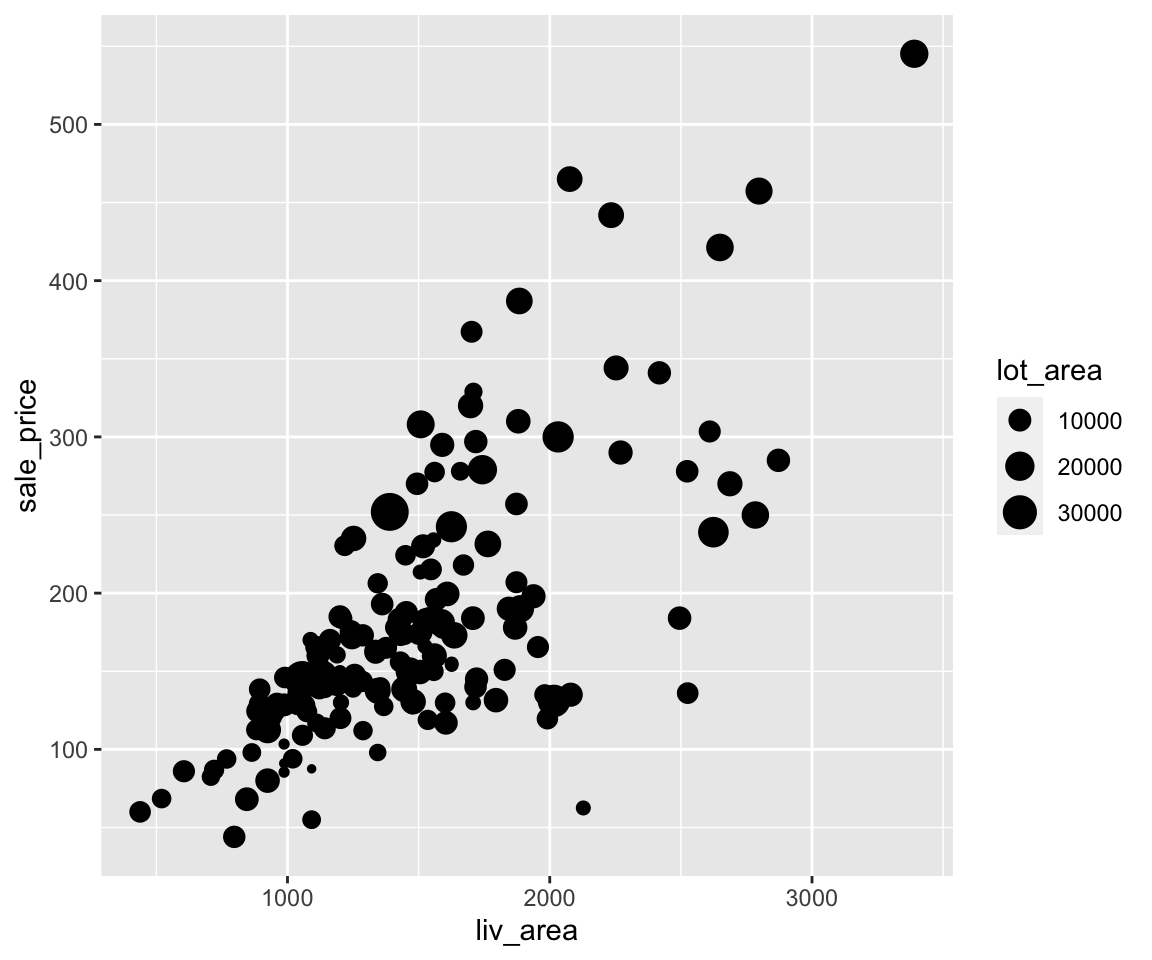
\includegraphics{bookdown-demo_files/figure-latex/unnamed-chunk-165-1.pdf}

Now, the two-story houses are triangles and other houses are circles.

Clearly, you can easily create new logical variables using any logical operations on existing variables, and map them into any aesthetics just like the existing categorical variables.í

\hypertarget{smoothline}{%
\section{Smoothline Fits}\label{smoothline}}

Now, you know how to create scatterplots with many possible customizations via specifying different aesthetics. In addition to scatterplots, a very useful type of plots that can capture the trend of pairwise relationship is the \textbf{smoothline fits}.

\hypertarget{creating-smoothline-fits-using-geom_smooth}{%
\subsection{\texorpdfstring{Creating Smoothline Fits using \texttt{geom\_smooth()}}{Creating Smoothline Fits using geom\_smooth()}}\label{creating-smoothline-fits-using-geom_smooth}}

To create a smoothline fit, you can use the \texttt{geom\_smooth()} function in the \textbf{ggplot2} package. Let's say you want to find the trend between the sale price and the living area of a house.

\begin{Shaded}
\begin{Highlighting}[]
\FunctionTok{library}\NormalTok{(ggplot2)}
\FunctionTok{library}\NormalTok{(r02pro)}
\FunctionTok{ggplot}\NormalTok{(}\AttributeTok{data =}\NormalTok{ sahp) }\SpecialCharTok{+} \FunctionTok{geom\_smooth}\NormalTok{(}\AttributeTok{mapping =} \FunctionTok{aes}\NormalTok{(}\AttributeTok{x =}\NormalTok{ liv\_area, }\AttributeTok{y =}\NormalTok{ sale\_price))}
\end{Highlighting}
\end{Shaded}

\begin{verbatim}
#> `geom_smooth()` using method = 'loess' and formula 'y ~ x'
\end{verbatim}

\begin{verbatim}
#> Warning: Removed 1 rows containing non-finite values (stat_smooth).
\end{verbatim}

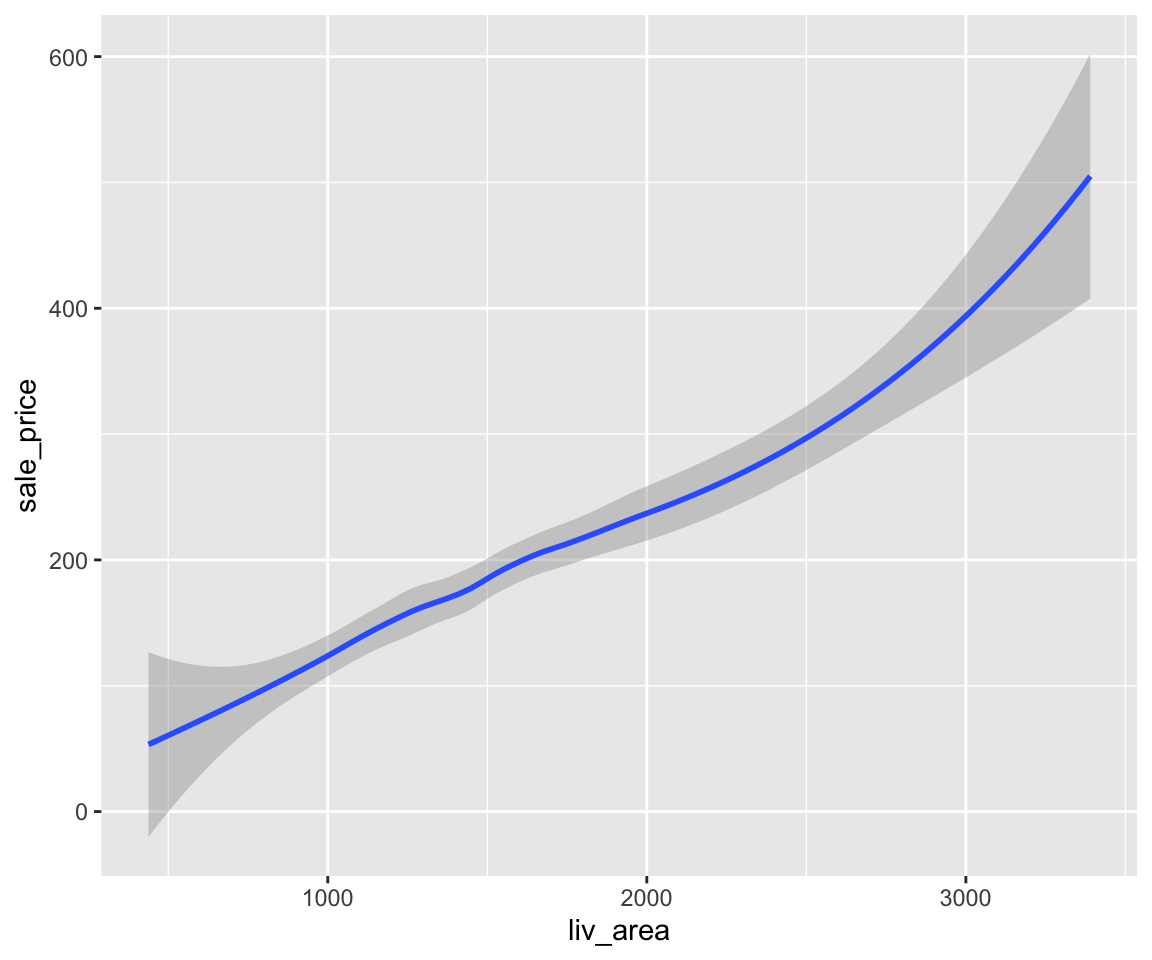
\includegraphics{bookdown-demo_files/figure-latex/unnamed-chunk-166-1.pdf}
Perhaps it is helpful to review the code for generating a scatterplot between \texttt{liv\_area} and \texttt{sale\_price}.

\begin{Shaded}
\begin{Highlighting}[]
\FunctionTok{ggplot}\NormalTok{(}\AttributeTok{data =}\NormalTok{ sahp) }\SpecialCharTok{+} \FunctionTok{geom\_point}\NormalTok{(}\AttributeTok{mapping =} \FunctionTok{aes}\NormalTok{(}\AttributeTok{x =}\NormalTok{ liv\_area, }\AttributeTok{y =}\NormalTok{ sale\_price))}
\end{Highlighting}
\end{Shaded}

We can see that the only difference is the use of different geoms. In fact, the mechanism of \texttt{geom\_smooth()} is that it fits a smooth line according to the points of the given variable pair. By default, it uses the \textbf{loess} method (locally estimated scatterplot smoothing), which is a popular nonparametric regression technique. In addition to the smoothline, it also generates a shaded area, representing the confidence interval around the fitted smoothline. To hide this shaded area, you can add the argument \texttt{se\ =\ FALSE} as a global aesthetic.

\begin{Shaded}
\begin{Highlighting}[]
\FunctionTok{ggplot}\NormalTok{(}\AttributeTok{data =}\NormalTok{ sahp) }\SpecialCharTok{+} \FunctionTok{geom\_smooth}\NormalTok{(}\AttributeTok{mapping =} \FunctionTok{aes}\NormalTok{(}\AttributeTok{x =}\NormalTok{ liv\_area, }\AttributeTok{y =}\NormalTok{ sale\_price), }\AttributeTok{se =} \ConstantTok{FALSE}\NormalTok{)}
\end{Highlighting}
\end{Shaded}

In addition to the default loess method for smoothline fit, \texttt{geom\_smooth()} also provides other smoothing moethods. For example, we can set \texttt{method\ =\ "lm"} to fit a linear line.

\begin{Shaded}
\begin{Highlighting}[]
\FunctionTok{ggplot}\NormalTok{(}\AttributeTok{data =}\NormalTok{ sahp) }\SpecialCharTok{+} \FunctionTok{geom\_smooth}\NormalTok{(}\AttributeTok{mapping =} \FunctionTok{aes}\NormalTok{(}\AttributeTok{x =}\NormalTok{ liv\_area, }\AttributeTok{y =}\NormalTok{ sale\_price), }\AttributeTok{method =} \StringTok{"lm"}\NormalTok{)}
\end{Highlighting}
\end{Shaded}

\begin{verbatim}
#> `geom_smooth()` using formula 'y ~ x'
\end{verbatim}

\begin{verbatim}
#> Warning: Removed 1 rows containing non-finite values (stat_smooth).
\end{verbatim}

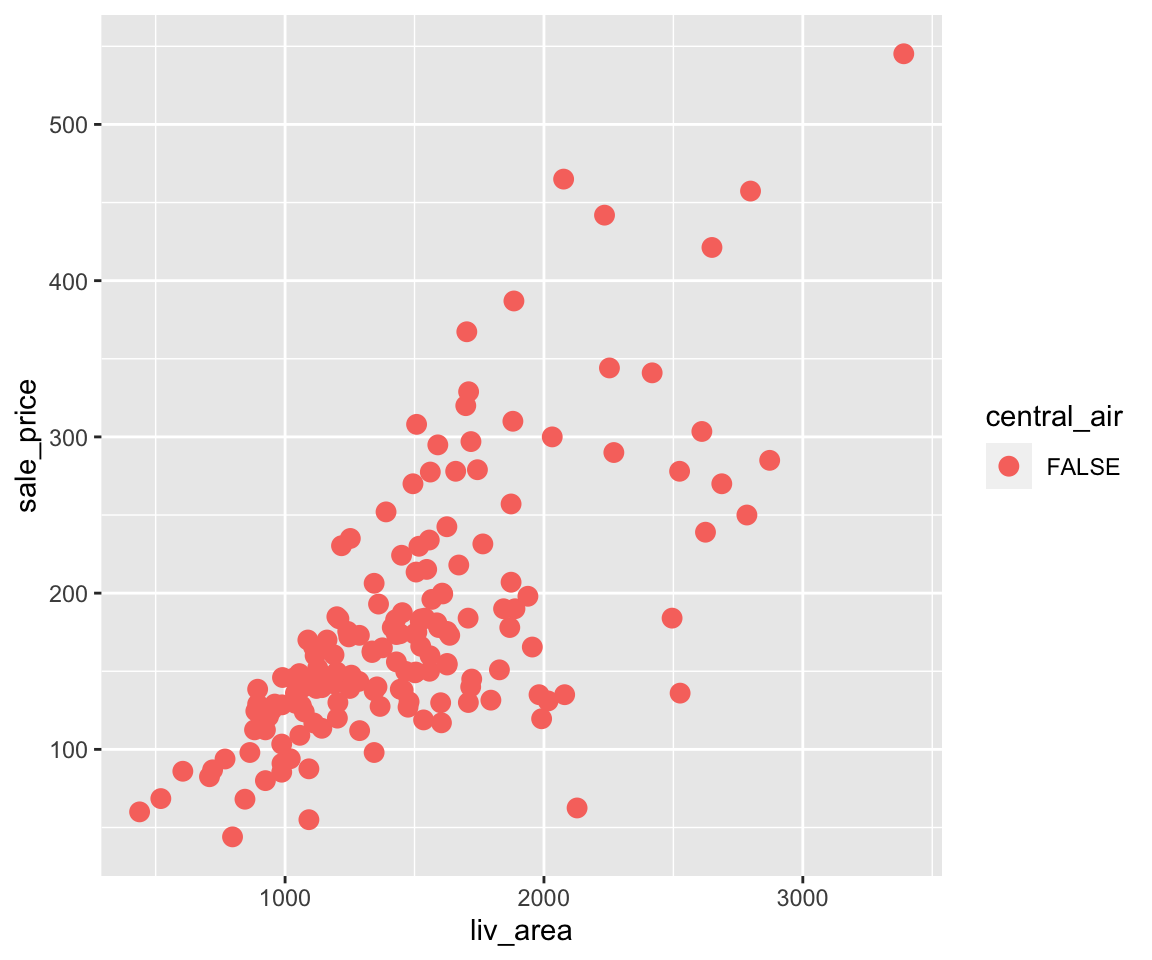
\includegraphics{bookdown-demo_files/figure-latex/unnamed-chunk-169-1.pdf}

\hypertarget{aesthetics-in-smoothline-fits}{%
\subsection{Aesthetics in Smoothline Fits}\label{aesthetics-in-smoothline-fits}}

As in scatterplots, you can also set global aesthetics as well as map variables to aesthetics in smoothline fits. Let's begin with mapping variables to aesthetics. We first define a new logical vector \texttt{good\_qual} which is \texttt{TRUE} when \texttt{oa\_qual\ \textgreater{}\ 5}.

\begin{Shaded}
\begin{Highlighting}[]
\NormalTok{sahp}\SpecialCharTok{$}\NormalTok{good\_qual }\OtherTok{\textless{}{-}}\NormalTok{ sahp}\SpecialCharTok{$}\NormalTok{oa\_qual }\SpecialCharTok{\textgreater{}} \DecValTok{5} 
\end{Highlighting}
\end{Shaded}

\textbf{\emph{a. Group}}

When we map a variable to the \texttt{group} aesthetic, \texttt{geom\_smooth} will first divide all the data points into different \emph{groups} according to the variable value, and then fit a separate smoothline for each group.

\begin{Shaded}
\begin{Highlighting}[]
\FunctionTok{ggplot}\NormalTok{(}\AttributeTok{data =}\NormalTok{ sahp) }\SpecialCharTok{+} \FunctionTok{geom\_smooth}\NormalTok{(}\AttributeTok{mapping =} \FunctionTok{aes}\NormalTok{(}\AttributeTok{x =}\NormalTok{ liv\_area, }\AttributeTok{y =}\NormalTok{ sale\_price, }\AttributeTok{group =}\NormalTok{ good\_qual))}
\end{Highlighting}
\end{Shaded}

\begin{verbatim}
#> `geom_smooth()` using method = 'loess' and formula 'y ~ x'
\end{verbatim}

\begin{verbatim}
#> Warning: Removed 1 rows containing non-finite values (stat_smooth).
\end{verbatim}

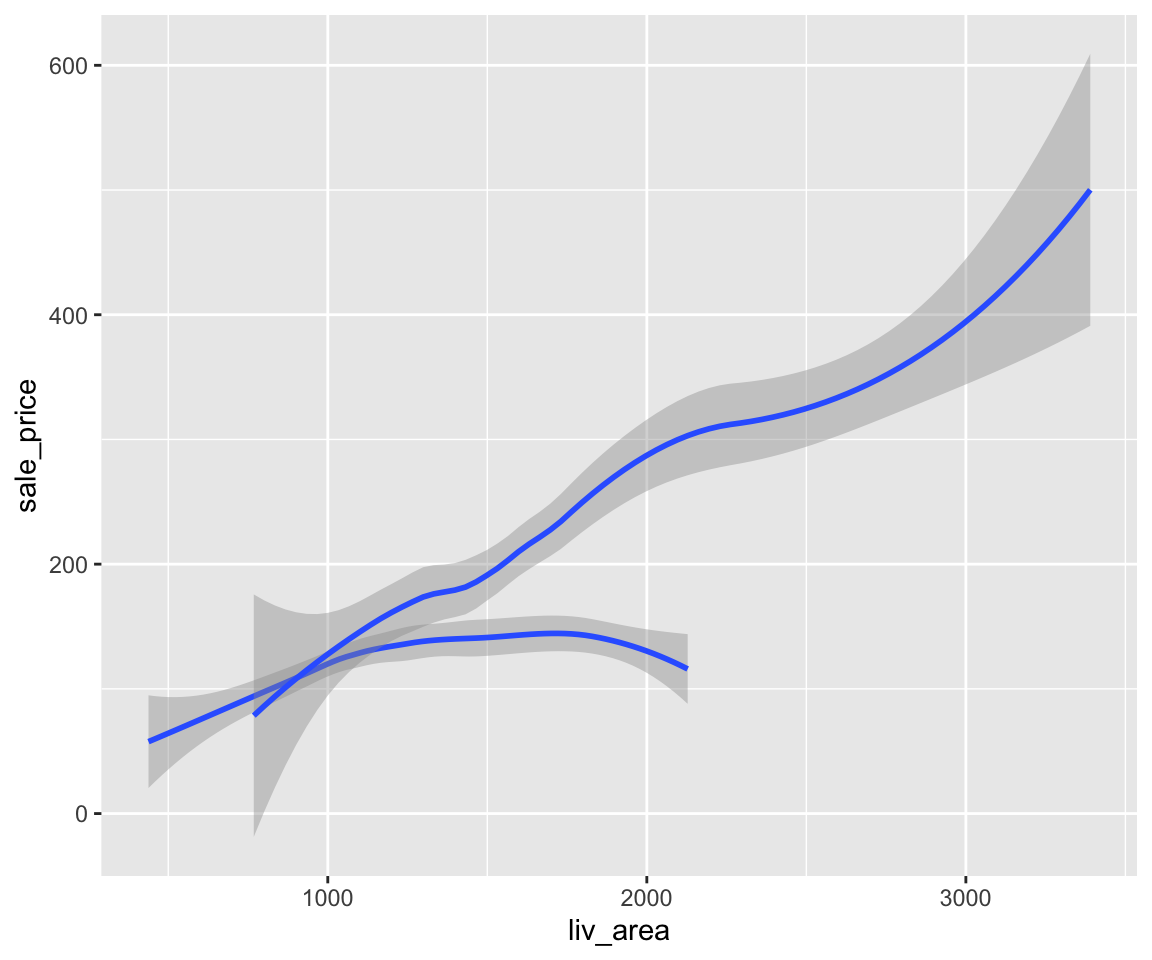
\includegraphics{bookdown-demo_files/figure-latex/unnamed-chunk-171-1.pdf}

You can see that two smoothlines are generated. However, it is not clear from the plot which group each smoothline corresponds to. To make the two smoothlines different, you can map the variable to other aesthetics.

\textbf{\emph{b. Color}}

As in \texttt{geom\_point()}, we can map the variable to the color aesthetic.

\begin{Shaded}
\begin{Highlighting}[]
\FunctionTok{ggplot}\NormalTok{(}\AttributeTok{data =}\NormalTok{ sahp) }\SpecialCharTok{+} \FunctionTok{geom\_smooth}\NormalTok{(}\AttributeTok{mapping =} \FunctionTok{aes}\NormalTok{(}\AttributeTok{x =}\NormalTok{ liv\_area, }\AttributeTok{y =}\NormalTok{ sale\_price, }\AttributeTok{color =}\NormalTok{ good\_qual))}
\end{Highlighting}
\end{Shaded}

\begin{verbatim}
#> `geom_smooth()` using method = 'loess' and formula 'y ~ x'
\end{verbatim}

\begin{verbatim}
#> Warning: Removed 1 rows containing non-finite values (stat_smooth).
\end{verbatim}

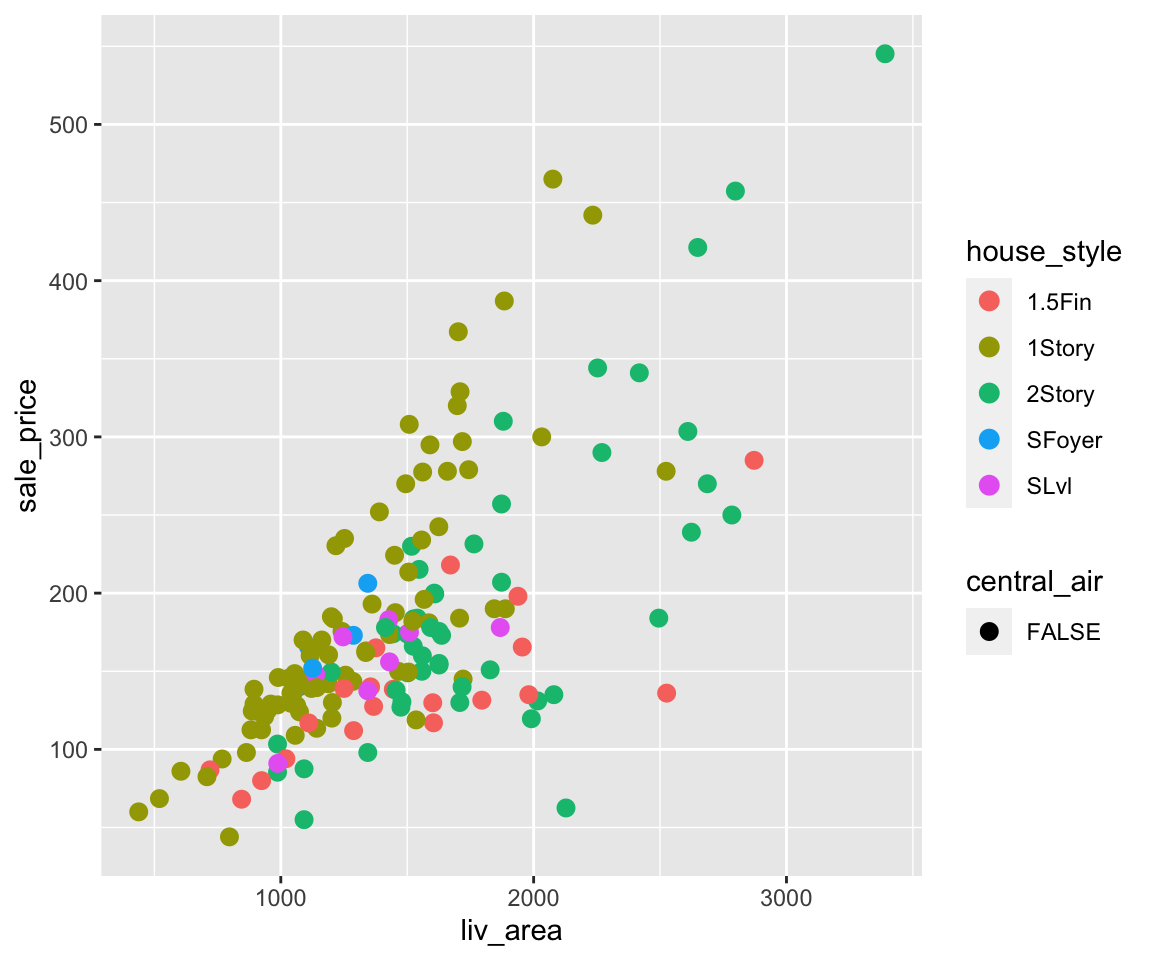
\includegraphics{bookdown-demo_files/figure-latex/unnamed-chunk-172-1.pdf}
This is a more informative plot than the one using \texttt{group} aesthetic as you can see the two smoothlines have different colors according to the \texttt{good\_qual} variable.ß

\textbf{\emph{c.~Linetype}}

Another useful aesthetic that was not applicable in \texttt{geom\_point()} is \texttt{linetype}, which controls the linetypes for each smoothline.

\begin{Shaded}
\begin{Highlighting}[]
\FunctionTok{ggplot}\NormalTok{(}\AttributeTok{data =}\NormalTok{ sahp) }\SpecialCharTok{+} \FunctionTok{geom\_smooth}\NormalTok{(}\AttributeTok{mapping =} \FunctionTok{aes}\NormalTok{(}\AttributeTok{x =}\NormalTok{ liv\_area, }\AttributeTok{y =}\NormalTok{ sale\_price, }\AttributeTok{linetype =}\NormalTok{ good\_qual))}
\end{Highlighting}
\end{Shaded}

\begin{verbatim}
#> `geom_smooth()` using method = 'loess' and formula 'y ~ x'
\end{verbatim}

\begin{verbatim}
#> Warning: Removed 1 rows containing non-finite values (stat_smooth).
\end{verbatim}

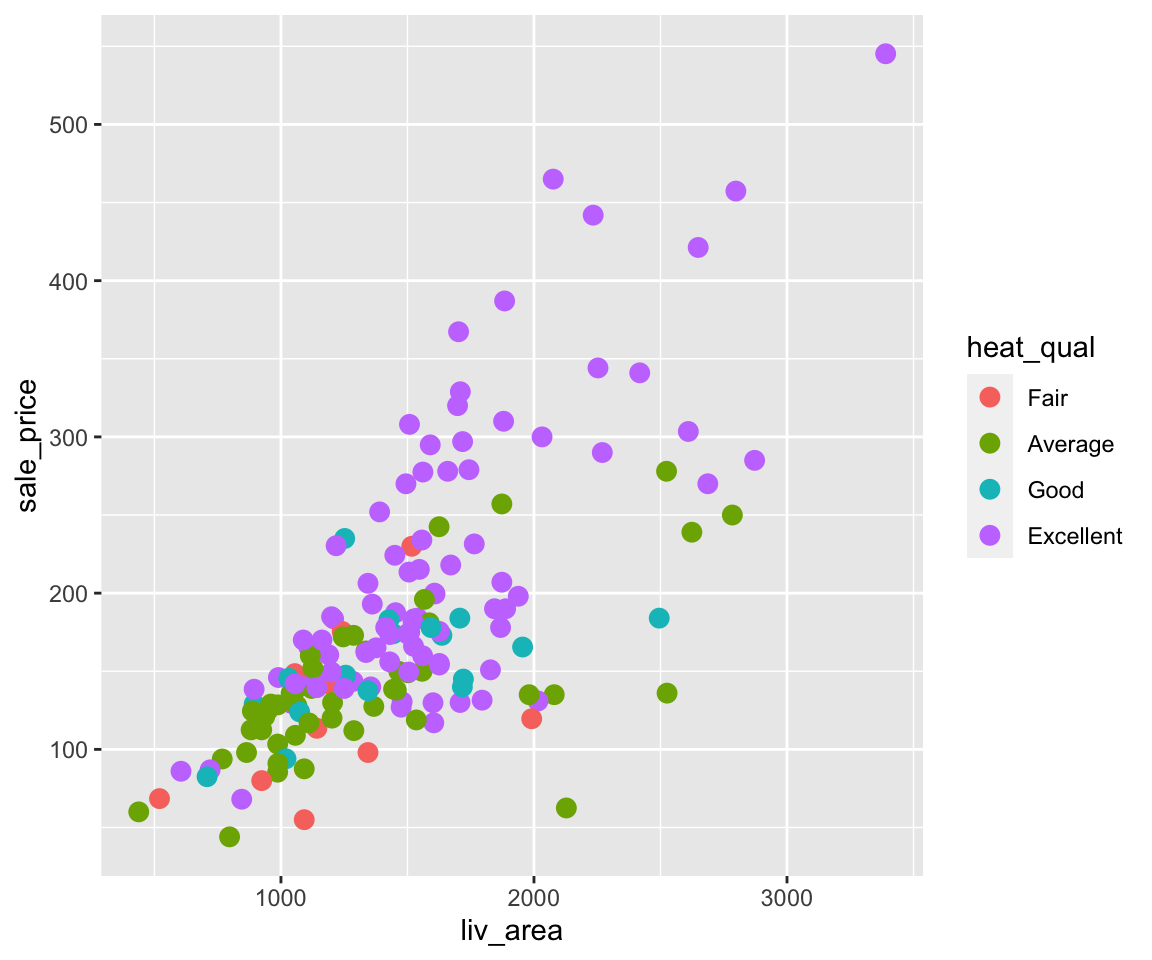
\includegraphics{bookdown-demo_files/figure-latex/unnamed-chunk-173-1.pdf}
The plot shows a dashed line for the smoothline corresponding to \texttt{good\_qual\ ==\ TRUE}, and a solid line for the smoothline corresponding to \texttt{good\_qual\ ==\ FALSE}.

\textbf{\emph{d.~Size}}

You can also map \texttt{good\_qual} to the \texttt{size} aesthetic, which controls the width of each smoothline fit.

\begin{Shaded}
\begin{Highlighting}[]
\FunctionTok{ggplot}\NormalTok{(}\AttributeTok{data =}\NormalTok{ sahp) }\SpecialCharTok{+} \FunctionTok{geom\_smooth}\NormalTok{(}\AttributeTok{mapping =} \FunctionTok{aes}\NormalTok{(}\AttributeTok{x =}\NormalTok{ liv\_area, }\AttributeTok{y =}\NormalTok{ sale\_price, }\AttributeTok{size =}\NormalTok{ good\_qual))}
\end{Highlighting}
\end{Shaded}

\begin{verbatim}
#> Warning: Using size for a discrete variable is not advised.
\end{verbatim}

\begin{verbatim}
#> `geom_smooth()` using method = 'loess' and formula 'y ~ x'
\end{verbatim}

\begin{verbatim}
#> Warning: Removed 1 rows containing non-finite values (stat_smooth).
\end{verbatim}

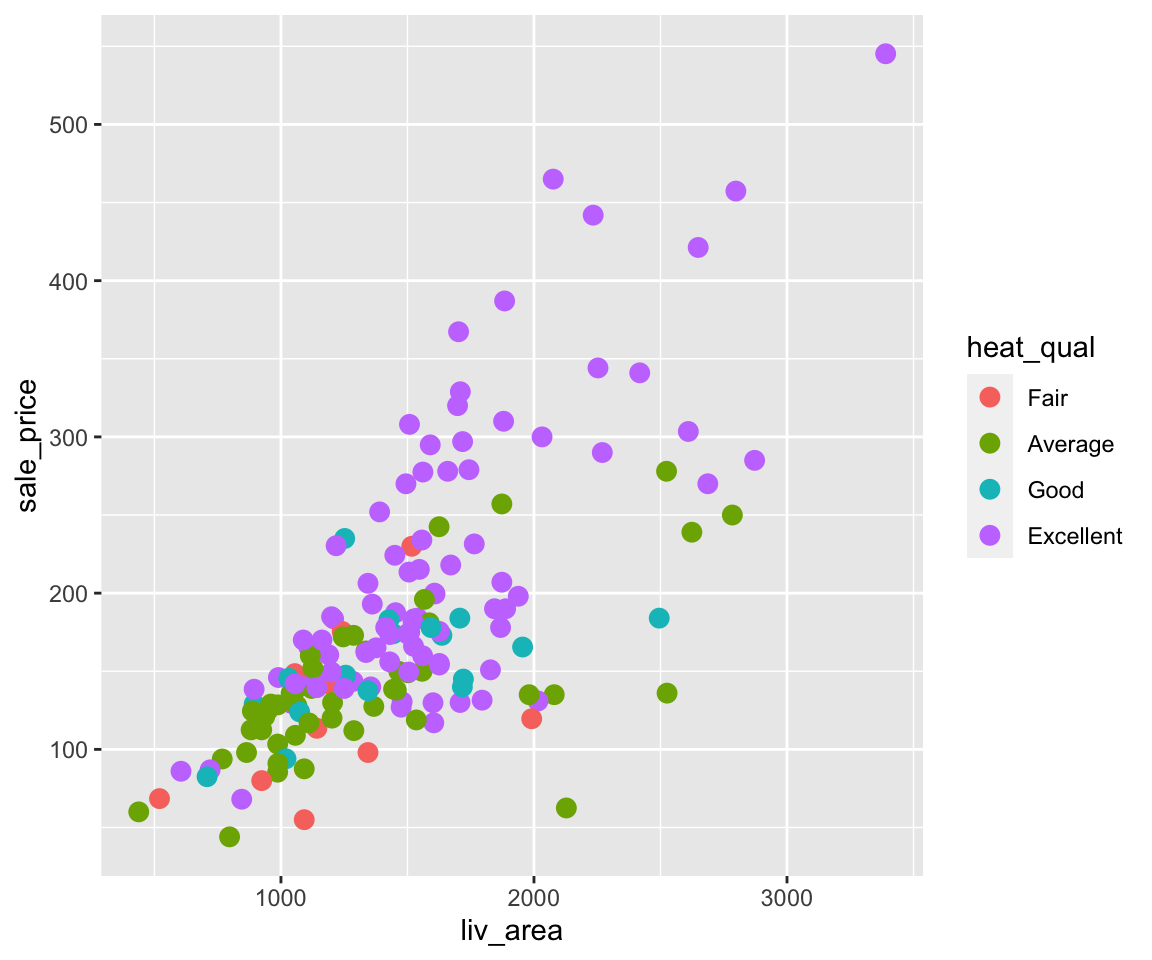
\includegraphics{bookdown-demo_files/figure-latex/unnamed-chunk-174-1.pdf}

It is worth to mention that \texttt{shape} is not a valid aesthetic for \texttt{geom\_smooth} as it doesn't make sense to talk about the shape of a line.

\begin{Shaded}
\begin{Highlighting}[]
\FunctionTok{ggplot}\NormalTok{(}\AttributeTok{data =}\NormalTok{ sahp) }\SpecialCharTok{+} \FunctionTok{geom\_smooth}\NormalTok{(}\AttributeTok{mapping =} \FunctionTok{aes}\NormalTok{(}\AttributeTok{x =}\NormalTok{ liv\_area, }\AttributeTok{y =}\NormalTok{ sale\_price, }\AttributeTok{shape =}\NormalTok{ good\_qual))}
\end{Highlighting}
\end{Shaded}

\begin{verbatim}
#> Warning: Ignoring unknown aesthetics: shape
\end{verbatim}

\begin{verbatim}
#> `geom_smooth()` using method = 'loess' and formula 'y ~ x'
\end{verbatim}

\begin{verbatim}
#> Warning: Removed 1 rows containing non-finite values (stat_smooth).
\end{verbatim}

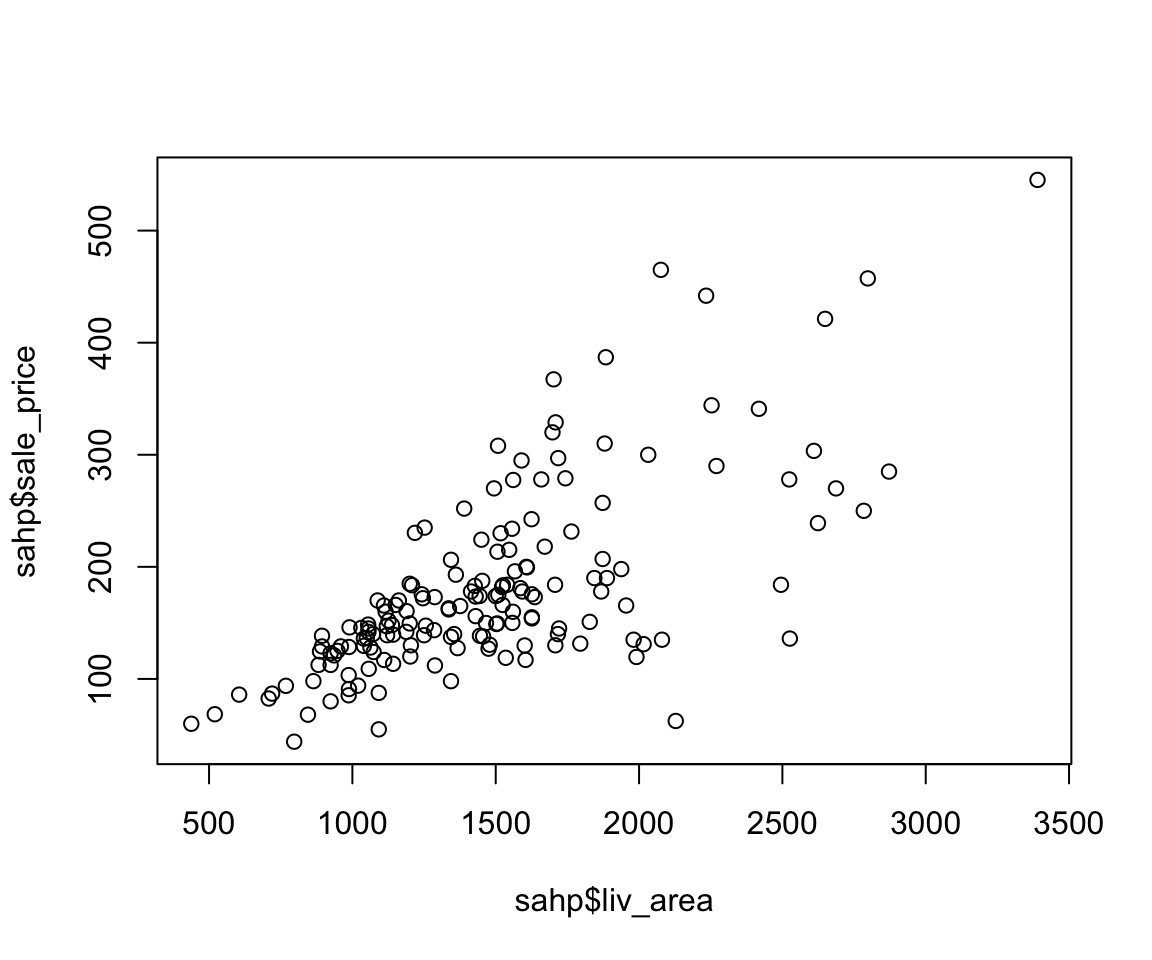
\includegraphics{bookdown-demo_files/figure-latex/unnamed-chunk-175-1.pdf}
When you tried to map a variable to the \texttt{shape} aesthetic, \texttt{geom\_smooth()} will show a warning message ``Warning: Ignoring unknown aesthetics: shape'', and use the \texttt{group} aesthetic instead.

Naturally, we can also have global aesthetic and it is straightforward to combine multiple aesthetics in the same plot.

\begin{Shaded}
\begin{Highlighting}[]
\FunctionTok{ggplot}\NormalTok{(}\AttributeTok{data =}\NormalTok{ sahp) }\SpecialCharTok{+} \FunctionTok{geom\_smooth}\NormalTok{(}\AttributeTok{mapping =} \FunctionTok{aes}\NormalTok{(}\AttributeTok{x =}\NormalTok{ liv\_area, }\AttributeTok{y =}\NormalTok{ sale\_price, }\AttributeTok{color =}\NormalTok{ good\_qual), }\AttributeTok{linetype =} \DecValTok{2}\NormalTok{)}
\end{Highlighting}
\end{Shaded}

\begin{verbatim}
#> `geom_smooth()` using method = 'loess' and formula 'y ~ x'
\end{verbatim}

\begin{verbatim}
#> Warning: Removed 1 rows containing non-finite values (stat_smooth).
\end{verbatim}

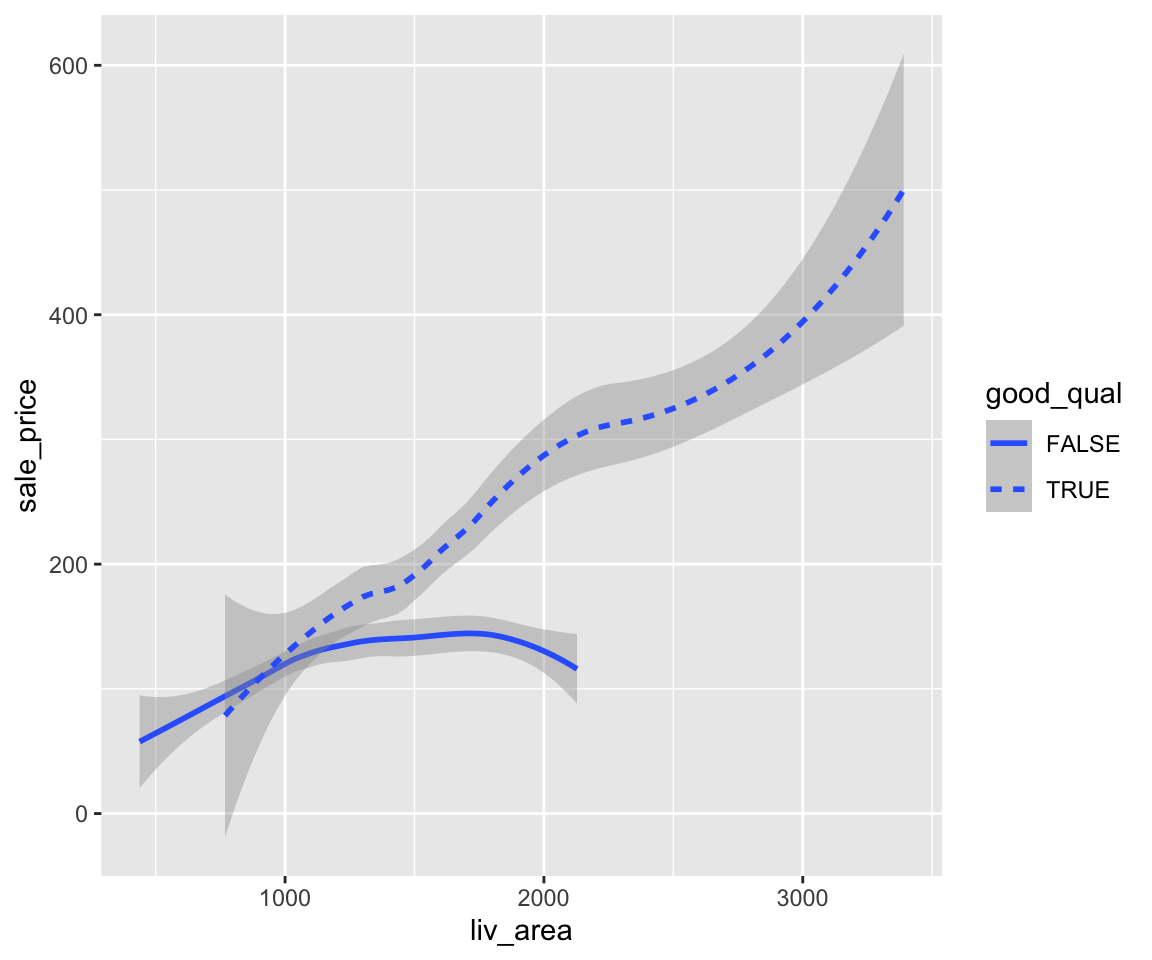
\includegraphics{bookdown-demo_files/figure-latex/unnamed-chunk-176-1.pdf}

\hypertarget{multi-geom}{%
\section{Multiple geoms and Aesthetics}\label{multi-geom}}

So far, you have learned to create scatterplots using \texttt{geom\_point()} and smoothline fits using \texttt{geom\_smooth()}. It is sometimes useful to combine multiple geoms in the same plot.

Let's first review the scatterplot and smoothline fit between \texttt{liv\_area} and \texttt{sale\_price}.

\begin{Shaded}
\begin{Highlighting}[]
\FunctionTok{library}\NormalTok{(r02pro)}
\FunctionTok{library}\NormalTok{(tidyverse)}
\FunctionTok{ggplot}\NormalTok{(}\AttributeTok{data =}\NormalTok{ sahp) }\SpecialCharTok{+} \FunctionTok{geom\_point}\NormalTok{(}\AttributeTok{mapping =} \FunctionTok{aes}\NormalTok{(}\AttributeTok{x =}\NormalTok{ liv\_area, }\AttributeTok{y =}\NormalTok{ sale\_price))}
\end{Highlighting}
\end{Shaded}

\begin{verbatim}
#> Warning: Removed 1 rows containing missing values (geom_point).
\end{verbatim}

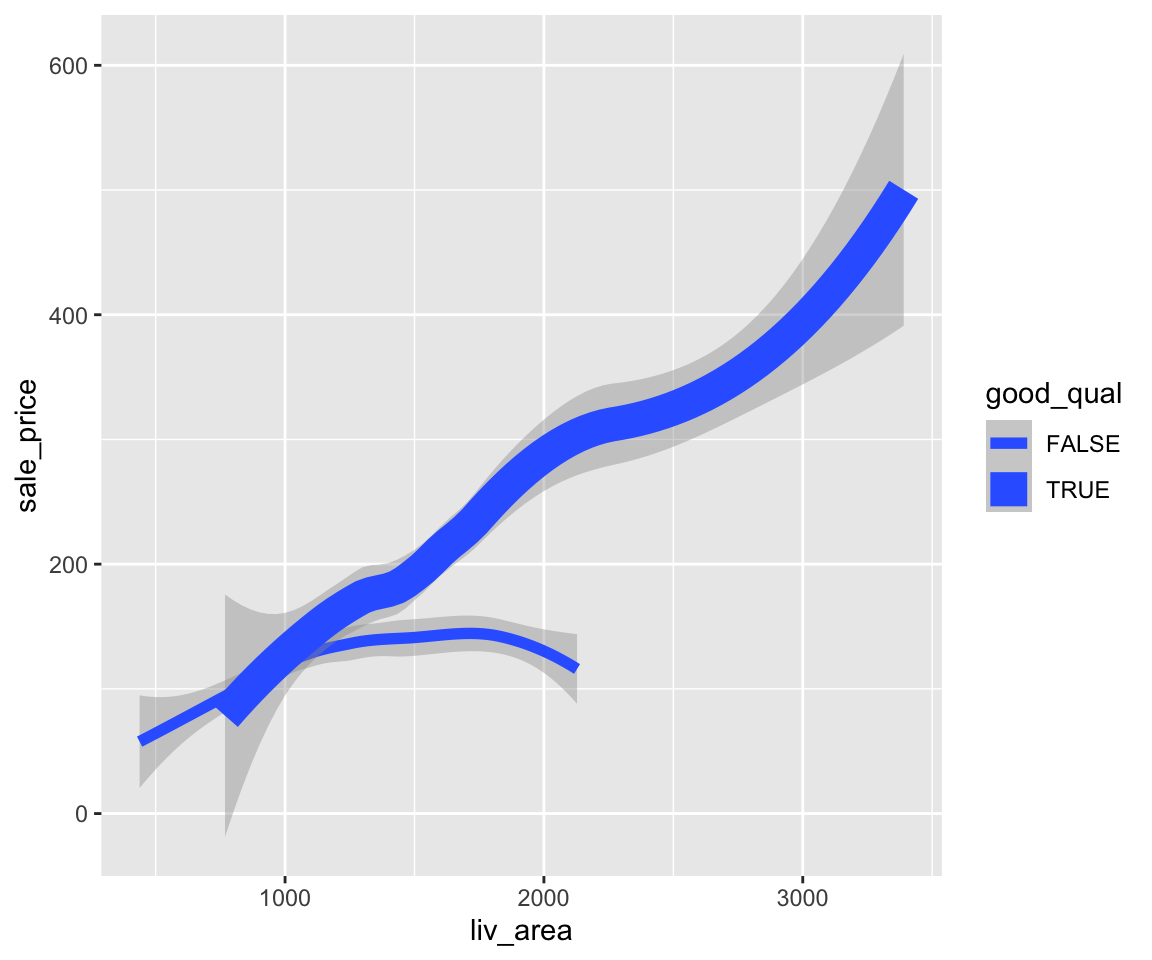
\includegraphics{bookdown-demo_files/figure-latex/unnamed-chunk-177-1.pdf}

\begin{Shaded}
\begin{Highlighting}[]
\FunctionTok{ggplot}\NormalTok{(}\AttributeTok{data =}\NormalTok{ sahp) }\SpecialCharTok{+} \FunctionTok{geom\_smooth}\NormalTok{(}\AttributeTok{mapping =} \FunctionTok{aes}\NormalTok{(}\AttributeTok{x =}\NormalTok{ liv\_area, }\AttributeTok{y =}\NormalTok{ sale\_price))}
\end{Highlighting}
\end{Shaded}

\begin{verbatim}
#> `geom_smooth()` using method = 'loess' and formula 'y ~ x'
\end{verbatim}

\begin{verbatim}
#> Warning: Removed 1 rows containing non-finite values (stat_smooth).
\end{verbatim}

\includegraphics{bookdown-demo_files/figure-latex/unnamed-chunk-177-2.pdf}

To combine multiple geoms, you can simply use \texttt{+} to add them.

\begin{Shaded}
\begin{Highlighting}[]
\FunctionTok{ggplot}\NormalTok{(}\AttributeTok{data =}\NormalTok{ sahp) }\SpecialCharTok{+} \FunctionTok{geom\_point}\NormalTok{(}\AttributeTok{mapping =} \FunctionTok{aes}\NormalTok{(}\AttributeTok{x =}\NormalTok{ liv\_area, }\AttributeTok{y =}\NormalTok{ sale\_price)) }\SpecialCharTok{+} \FunctionTok{geom\_smooth}\NormalTok{(}\AttributeTok{mapping =} \FunctionTok{aes}\NormalTok{(}\AttributeTok{x =}\NormalTok{ liv\_area, }\AttributeTok{y =}\NormalTok{ sale\_price))}
\end{Highlighting}
\end{Shaded}

\begin{verbatim}
#> `geom_smooth()` using method = 'loess' and formula 'y ~ x'
\end{verbatim}

\begin{verbatim}
#> Warning: Removed 1 rows containing non-finite values (stat_smooth).
\end{verbatim}

\begin{verbatim}
#> Warning: Removed 1 rows containing missing values (geom_point).
\end{verbatim}

\includegraphics{bookdown-demo_files/figure-latex/unnamed-chunk-178-1.pdf}
As expected, you see all the points and the smoothline fit on the same plot, which contains very rich information.

As usual, you can add aesthetics to both geoms.

Let's first map \texttt{good\_qual} (defined as \texttt{oa\_qual\ \textgreater{}\ 5} in Section \ref{smoothline}) to the color aesthetic for \texttt{geom\_smooth()}.

\begin{Shaded}
\begin{Highlighting}[]
\FunctionTok{ggplot}\NormalTok{(}\AttributeTok{data =}\NormalTok{ sahp) }\SpecialCharTok{+} \FunctionTok{geom\_point}\NormalTok{(}\AttributeTok{mapping =} \FunctionTok{aes}\NormalTok{(}\AttributeTok{x =}\NormalTok{ liv\_area, }\AttributeTok{y =}\NormalTok{ sale\_price)) }\SpecialCharTok{+} \FunctionTok{geom\_smooth}\NormalTok{(}\AttributeTok{mapping =} \FunctionTok{aes}\NormalTok{(}\AttributeTok{x =}\NormalTok{ liv\_area, }\AttributeTok{y =}\NormalTok{ sale\_price, }\AttributeTok{color =}\NormalTok{ good\_qual))}
\end{Highlighting}
\end{Shaded}

\begin{verbatim}
#> `geom_smooth()` using method = 'loess' and formula 'y ~ x'
\end{verbatim}

\begin{verbatim}
#> Warning: Removed 1 rows containing non-finite values (stat_smooth).
\end{verbatim}

\begin{verbatim}
#> Warning: Removed 1 rows containing missing values (geom_point).
\end{verbatim}

\includegraphics{bookdown-demo_files/figure-latex/unnamed-chunk-179-1.pdf}

To verify the two smoothline fits are indeed fitted from the data points in the two groups, you can map \texttt{good\_qual} to the color aesthetic for \texttt{geom\_point()} as well.

\begin{Shaded}
\begin{Highlighting}[]
\FunctionTok{ggplot}\NormalTok{(}\AttributeTok{data =}\NormalTok{ sahp) }\SpecialCharTok{+} \FunctionTok{geom\_point}\NormalTok{(}\AttributeTok{mapping =} \FunctionTok{aes}\NormalTok{(}\AttributeTok{x =}\NormalTok{ liv\_area, }\AttributeTok{y =}\NormalTok{ sale\_price, }\AttributeTok{color =}\NormalTok{ good\_qual)) }\SpecialCharTok{+} \FunctionTok{geom\_smooth}\NormalTok{(}\AttributeTok{mapping =} \FunctionTok{aes}\NormalTok{(}\AttributeTok{x =}\NormalTok{ liv\_area, }\AttributeTok{y =}\NormalTok{ sale\_price, }\AttributeTok{color =}\NormalTok{ good\_qual), }\AttributeTok{se =} \ConstantTok{FALSE}\NormalTok{)}
\end{Highlighting}
\end{Shaded}

\begin{verbatim}
#> `geom_smooth()` using method = 'loess' and formula 'y ~ x'
\end{verbatim}

\begin{verbatim}
#> Warning: Removed 1 rows containing non-finite values (stat_smooth).
\end{verbatim}

\begin{verbatim}
#> Warning: Removed 1 rows containing missing values (geom_point).
\end{verbatim}

\includegraphics{bookdown-demo_files/figure-latex/unnamed-chunk-180-1.pdf}
The plot is reassuring that the two smoothline fits indeed correspond to the data points in the two groups defined by \texttt{good\_qual}. Note that the legend also shows a \texttt{NA} category since there is a missing value in the variable \texttt{good\_qual}.

In addition to mapping variables to aesthetics, you can also use global aesthetics.

\begin{Shaded}
\begin{Highlighting}[]
\FunctionTok{ggplot}\NormalTok{(}\AttributeTok{data =}\NormalTok{ sahp) }\SpecialCharTok{+} \FunctionTok{geom\_point}\NormalTok{(}\AttributeTok{mapping =} \FunctionTok{aes}\NormalTok{(}\AttributeTok{x =}\NormalTok{ liv\_area, }\AttributeTok{y =}\NormalTok{ sale\_price, }\AttributeTok{color =}\NormalTok{ good\_qual, }\AttributeTok{shape =}\NormalTok{ house\_style }\SpecialCharTok{==} \StringTok{"2Story"}\NormalTok{)) }\SpecialCharTok{+} \FunctionTok{geom\_smooth}\NormalTok{(}\AttributeTok{mapping =} \FunctionTok{aes}\NormalTok{(}\AttributeTok{x =}\NormalTok{ liv\_area, }\AttributeTok{y =}\NormalTok{ sale\_price, }\AttributeTok{color =}\NormalTok{ good\_qual), }\AttributeTok{linetype =} \DecValTok{2}\NormalTok{, }\AttributeTok{se =} \ConstantTok{FALSE}\NormalTok{)}
\end{Highlighting}
\end{Shaded}

\begin{verbatim}
#> `geom_smooth()` using method = 'loess' and formula 'y ~ x'
\end{verbatim}

\begin{verbatim}
#> Warning: Removed 1 rows containing non-finite values (stat_smooth).
\end{verbatim}

\begin{verbatim}
#> Warning: Removed 1 rows containing missing values (geom_point).
\end{verbatim}

\includegraphics{bookdown-demo_files/figure-latex/unnamed-chunk-181-1.pdf}

\hypertarget{global-local-mapping}{%
\section{Global and Local Aesthetic Mappings}\label{global-local-mapping}}

In Section \ref{multi-geom}, you learned how to combine the scatterplot and smoothline fit into a single plot by using two geoms.

Let's first review the code.

\begin{Shaded}
\begin{Highlighting}[]
\FunctionTok{library}\NormalTok{(r02pro)}
\FunctionTok{library}\NormalTok{(tidyverse)}
\FunctionTok{ggplot}\NormalTok{(}\AttributeTok{data =}\NormalTok{ sahp) }\SpecialCharTok{+} \FunctionTok{geom\_point}\NormalTok{(}\AttributeTok{mapping =} \FunctionTok{aes}\NormalTok{(}\AttributeTok{x =}\NormalTok{ liv\_area, }\AttributeTok{y =}\NormalTok{ sale\_price)) }\SpecialCharTok{+} \FunctionTok{geom\_smooth}\NormalTok{(}\AttributeTok{mapping =} \FunctionTok{aes}\NormalTok{(}\AttributeTok{x =}\NormalTok{ liv\_area, }\AttributeTok{y =}\NormalTok{ sale\_price))}
\end{Highlighting}
\end{Shaded}

\begin{verbatim}
#> `geom_smooth()` using method = 'loess' and formula 'y ~ x'
\end{verbatim}

\begin{verbatim}
#> Warning: Removed 1 rows containing non-finite values (stat_smooth).
\end{verbatim}

\begin{verbatim}
#> Warning: Removed 1 rows containing missing values (geom_point).
\end{verbatim}

\includegraphics{bookdown-demo_files/figure-latex/unnamed-chunk-182-1.pdf}

You may notice that the arguments inside \texttt{geom\_point()} and \texttt{geom\_smooth()} are identical. Now, thinking about if we want to generate another plot by replacing the \texttt{liv\_area} with \texttt{lot\_area} (the size of lot area), both instances of \texttt{liv\_area} need to be changed to \texttt{lot\_area}, which is a bit cumbersome. It turns out we can use the so-called \textbf{global mapping} to simplify the code. Correspondingly, we call a mapping inside a specific geom \textbf{local mapping}.

To use the global mapping, we move the \texttt{mapping} argument from the geoms into the \texttt{ggplot()} function.

\begin{Shaded}
\begin{Highlighting}[]
\FunctionTok{ggplot}\NormalTok{(}\AttributeTok{data =}\NormalTok{ sahp, }\AttributeTok{mapping =} \FunctionTok{aes}\NormalTok{(}\AttributeTok{x =}\NormalTok{ liv\_area, }\AttributeTok{y =}\NormalTok{ sale\_price)) }\SpecialCharTok{+} \FunctionTok{geom\_point}\NormalTok{() }\SpecialCharTok{+} \FunctionTok{geom\_smooth}\NormalTok{()}
\end{Highlighting}
\end{Shaded}

We can also map variables to aesthetics in the global mapping. The global aesthetic mapping will be inherited in all geoms used.

\begin{Shaded}
\begin{Highlighting}[]
\FunctionTok{ggplot}\NormalTok{(}\AttributeTok{data =}\NormalTok{ sahp, }\AttributeTok{mapping =} \FunctionTok{aes}\NormalTok{(}\AttributeTok{x =}\NormalTok{ lot\_area, }\AttributeTok{y =}\NormalTok{ sale\_price, }\AttributeTok{color =}\NormalTok{ kit\_qual)) }\SpecialCharTok{+} \FunctionTok{geom\_point}\NormalTok{() }\SpecialCharTok{+} \FunctionTok{geom\_smooth}\NormalTok{()}
\end{Highlighting}
\end{Shaded}

\begin{verbatim}
#> `geom_smooth()` using method = 'loess' and formula 'y ~ x'
\end{verbatim}

\begin{verbatim}
#> Warning: Removed 1 rows containing non-finite values (stat_smooth).
\end{verbatim}

\begin{verbatim}
#> Warning: Removed 1 rows containing missing values (geom_point).
\end{verbatim}

\includegraphics{bookdown-demo_files/figure-latex/unnamed-chunk-184-1.pdf}

Clearly, the use of global mapping greatly simplify our code as we would need to repeat the same mapping argument in both geoms.

In addition to use the same mapping in each geom as the global mapping, we can extend or overwrite the global mapping in each geom.

\begin{enumerate}
\def\labelenumi{\arabic{enumi}.}
\tightlist
\item
  Extend Global Aesthetic Mappings
\end{enumerate}

\begin{Shaded}
\begin{Highlighting}[]
\FunctionTok{ggplot}\NormalTok{(}\AttributeTok{data =}\NormalTok{ sahp, }\AttributeTok{mapping =} \FunctionTok{aes}\NormalTok{(}\AttributeTok{x =}\NormalTok{ lot\_area, }\AttributeTok{y =}\NormalTok{ sale\_price, }\AttributeTok{color =}\NormalTok{ kit\_qual)) }\SpecialCharTok{+} \FunctionTok{geom\_point}\NormalTok{(}\AttributeTok{mapping =} \FunctionTok{aes}\NormalTok{(}\AttributeTok{shape =}\NormalTok{ gar\_car }\SpecialCharTok{\textgreater{}} \DecValTok{1}\NormalTok{)) }\SpecialCharTok{+} \FunctionTok{geom\_smooth}\NormalTok{(}\AttributeTok{mapping =} \FunctionTok{aes}\NormalTok{(}\AttributeTok{linetype =}\NormalTok{ kit\_qual))}
\end{Highlighting}
\end{Shaded}

\begin{verbatim}
#> `geom_smooth()` using method = 'loess' and formula 'y ~ x'
\end{verbatim}

\includegraphics{bookdown-demo_files/figure-latex/unnamed-chunk-185-1.pdf}

\begin{enumerate}
\def\labelenumi{\arabic{enumi}.}
\setcounter{enumi}{1}
\tightlist
\item
  Overwrite Global Aesthetic Mappings
\end{enumerate}

\begin{Shaded}
\begin{Highlighting}[]
\FunctionTok{ggplot}\NormalTok{(}\AttributeTok{data =}\NormalTok{ sahp, }\AttributeTok{mapping =} \FunctionTok{aes}\NormalTok{(}\AttributeTok{x =}\NormalTok{ lot\_area, }\AttributeTok{y =}\NormalTok{ sale\_price, }\AttributeTok{color =}\NormalTok{ kit\_qual)) }\SpecialCharTok{+} \FunctionTok{geom\_point}\NormalTok{(}\AttributeTok{mapping =} \FunctionTok{aes}\NormalTok{(}\AttributeTok{color =}\NormalTok{ gar\_car }\SpecialCharTok{\textgreater{}} \DecValTok{1}\NormalTok{)) }\SpecialCharTok{+} \FunctionTok{geom\_smooth}\NormalTok{(}\AttributeTok{mapping =} \FunctionTok{aes}\NormalTok{(}\AttributeTok{color =}\NormalTok{ gar\_car }\SpecialCharTok{\textgreater{}} \DecValTok{1}\NormalTok{))}
\end{Highlighting}
\end{Shaded}

\begin{verbatim}
#> `geom_smooth()` using method = 'loess' and formula 'y ~ x'
\end{verbatim}

\includegraphics{bookdown-demo_files/figure-latex/unnamed-chunk-186-1.pdf}

\begin{enumerate}
\def\labelenumi{\arabic{enumi}.}
\setcounter{enumi}{2}
\tightlist
\item
  Mix
\end{enumerate}

\begin{Shaded}
\begin{Highlighting}[]
\FunctionTok{ggplot}\NormalTok{(}\AttributeTok{data =}\NormalTok{ sahp, }\AttributeTok{mapping =} \FunctionTok{aes}\NormalTok{(}\AttributeTok{x =}\NormalTok{ liv\_area, }\AttributeTok{y =}\NormalTok{ sale\_price, }\AttributeTok{color =}\NormalTok{ kit\_qual)) }\SpecialCharTok{+} \FunctionTok{geom\_point}\NormalTok{(}\AttributeTok{mapping =} \FunctionTok{aes}\NormalTok{(}\AttributeTok{shape =}\NormalTok{ house\_style }\SpecialCharTok{==} \StringTok{"2Story"}\NormalTok{), }\AttributeTok{size =} \DecValTok{2}\NormalTok{) }\SpecialCharTok{+} \FunctionTok{geom\_smooth}\NormalTok{(}\AttributeTok{linetype =} \DecValTok{2}\NormalTok{, }\AttributeTok{se =} \ConstantTok{FALSE}\NormalTok{)}
\end{Highlighting}
\end{Shaded}

\begin{verbatim}
#> `geom_smooth()` using method = 'loess' and formula 'y ~ x'
\end{verbatim}

\includegraphics{bookdown-demo_files/figure-latex/unnamed-chunk-187-1.pdf}

\hypertarget{import-export}{%
\chapter{Data Import and Export}\label{import-export}}

So far in this book, you have been creating objects by yourself or working with existing data in R packages. When working on a project, you often need to \textbf{import} existing data into R, or \textbf{export} the created object into a file on the computer. In this chapter, you will learn how to import and export data of different file types.

\hypertarget{export-data}{%
\section{Exporting Data to Delimited Files}\label{export-data}}

We will start by introducing how to export data to a file in this chapter.

\hypertarget{set-the-working-directory}{%
\subsection{Set the working directory}\label{set-the-working-directory}}

Firstly, we will introduce an important concept of \textbf{Working Directory}. To conduct the data export and import, you are recommended to set the \emph{working directory} since we usually use a path relative to the working directory for interacting with files on the computer in R, . To set the working directory, you can click \emph{Session} on the menu and click \emph{Set Working Directory}. \textbf{ADD a screenshot with this menu here} There are three options under this menu.

\begin{itemize}
\tightlist
\item
  \emph{To Source File Location}: this is the same directory as the current R script.
\item
  \emph{To Files Pane Location}: this is the same directory as shown in the Files Panel on the bottom right of RStudio.
\item
  \emph{Choose Directory\ldots{}}: this will open up a window from which you can choose any desired directory.
\end{itemize}

After selecting any of the three options, we can see a line of code containing the function \texttt{setwd()} executed in the console. \textbf{ADD a screenshot with this line of code here} Indeed, this menu operation is equivalent to using the \texttt{setwd()} function with the argument being the full path or relative path of the desired directory.

Another related function is \texttt{getwd()} which tells us the absolute path representing the current working directory.

\begin{Shaded}
\begin{Highlighting}[]
\FunctionTok{getwd}\NormalTok{()}
\end{Highlighting}
\end{Shaded}

\hypertarget{delimited-files}{%
\subsection{Delimited files}\label{delimited-files}}

In most applications, you will use a specific file type called \textbf{delimited} file. In a delimited file, each row represents a single observation, and it has values separated by the \textbf{delimiter}. In principle, \emph{any character (including letters, numbers, or symbols)} can be used as a delimiter, with the most commonly used ones being comma, tab, colon, and space.

\hypertarget{write-an-object-into-a-.csv-file}{%
\subsection{Write an object into a .csv file}\label{write-an-object-into-a-.csv-file}}

First, let's work with one popular kind of \emph{delimited} files called \emph{comma-separated value} file, usually with the file extension .csv. In a .csv file, the \emph{delimiter} is \emph{comma} (\texttt{,}).

Let's review the data frame you created in \textbf{Section???}.

\begin{Shaded}
\begin{Highlighting}[]
\NormalTok{dig\_num }\OtherTok{\textless{}{-}} \DecValTok{7}\SpecialCharTok{:}\DecValTok{1}
\NormalTok{ani\_char }\OtherTok{\textless{}{-}} \FunctionTok{c}\NormalTok{(}\StringTok{"sheep"}\NormalTok{, }\StringTok{"pig"}\NormalTok{, }\StringTok{"monkey"}\NormalTok{, }\StringTok{"pig"}\NormalTok{, }\StringTok{"monkey"}\NormalTok{, }\ConstantTok{NA}\NormalTok{, }\StringTok{"pig"}\NormalTok{)}
\NormalTok{conditions }\OtherTok{\textless{}{-}} \FunctionTok{c}\NormalTok{(}\StringTok{"Excellent"}\NormalTok{, }\StringTok{"Good"}\NormalTok{, }\StringTok{"N"}\NormalTok{, }\StringTok{"Fair"}\NormalTok{, }\StringTok{"Good"}\NormalTok{, }\StringTok{"Good"}\NormalTok{, }\StringTok{"Excellent"}\NormalTok{)}
\NormalTok{my\_animals}\OtherTok{\textless{}{-}} \FunctionTok{data.frame}\NormalTok{(dig\_num, ani\_char, conditions)}
\NormalTok{my\_animals}
\end{Highlighting}
\end{Shaded}

Now, let's write the data frame \texttt{my\_animals} into a file called ``my\_animals.csv'' in the currently working directory. To write an object into a .csv file, you will use the \texttt{write\_csv()} function in the \textbf{readr} package. Since \textbf{readr} is a subpackage of \textbf{tidyverse}, you don't need to install it separately, but you need to load the package in each new R session.

\begin{Shaded}
\begin{Highlighting}[]
\FunctionTok{library}\NormalTok{(readr)}
\FunctionTok{write\_csv}\NormalTok{(my\_animals, }\StringTok{"my\_animals.csv"}\NormalTok{)}
\end{Highlighting}
\end{Shaded}

You can verify the .csv file has been indeed created and open the file with RStudio or any text editor to verify its contents. \textbf{Shall we use a screenshot again?}
We can see that all the information has been written in the .csv file, which has \emph{commas} separating the values on each line. In particular, you may find out the first row of the file corresponds to the column names. If you don't want to include the column names, you can set the argument \texttt{col\_names} to be \texttt{FALSE}.

\begin{Shaded}
\begin{Highlighting}[]
\FunctionTok{write\_csv}\NormalTok{(my\_animals, }\StringTok{"my\_animals\_no\_colname.csv"}\NormalTok{, }\AttributeTok{col\_names =} \ConstantTok{FALSE}\NormalTok{)}
\end{Highlighting}
\end{Shaded}

By default, \texttt{write\_csv()} writes the data into a file in which \texttt{NA} is used to represent all the missing values, just like in the tibble. If you want to use another string to represent the missing values in the file, you can set the argument \texttt{na} to be the string.

\begin{Shaded}
\begin{Highlighting}[]
\FunctionTok{write\_csv}\NormalTok{(my\_animals, }\StringTok{"my\_animals\_missing.csv"}\NormalTok{, }\AttributeTok{na =} \StringTok{"This value is missing!"}\NormalTok{)}
\end{Highlighting}
\end{Shaded}

\hypertarget{write-an-object-into-a-delimited-file}{%
\subsection{Write an object into a delimited file}\label{write-an-object-into-a-delimited-file}}

As introduced at the beginning, there are different types of \emph{delimited files} depending on the specific \emph{delimiter}. The function \texttt{write\_delim()} enables us to write an object into a delimited file with any chosen delimiter. The usage of \texttt{write\_delim()} is almost identical to \texttt{write\_csv()}, except that it has an additional argument \texttt{delim}, which specifies the delimiter to be used. Let's see the following example with \texttt{*} as the delimiter.

\begin{Shaded}
\begin{Highlighting}[]
\FunctionTok{write\_delim}\NormalTok{(my\_animals, }\StringTok{"my\_animals\_star.csv"}\NormalTok{, }\AttributeTok{delim =} \StringTok{"*"}\NormalTok{)}
\end{Highlighting}
\end{Shaded}

\hypertarget{exercise-6}{%
\subsection{Exercise}\label{exercise-6}}

You can run the following code to do the exercise.

\begin{Shaded}
\begin{Highlighting}[]
\FunctionTok{r02pro}\NormalTok{(}\StringTok{"4"}\NormalTok{)}
\end{Highlighting}
\end{Shaded}

\hypertarget{import-data}{%
\section{Importing Data from Delimited Files}\label{import-data}}

Knowing how to export data into delimited files, let's see how to \textbf{import} data from the delimited files.

\hypertarget{import-.csv-files-using-read_csv}{%
\subsection{\texorpdfstring{Import .csv Files using \texttt{read\_csv()}}{Import .csv Files using read\_csv()}}\label{import-.csv-files-using-read_csv}}

To import .csv files, we can use the function \texttt{read\_csv()} in the \textbf{readr} package, which is a sub-package of \textbf{tidyverse}. If you have already installed \textbf{tidyverse}, you can directly load the \textbf{readr} package.

After loading the \textbf{readr} package, you can try to import the data from ``my\_animals.csv'', which you want to make sure is in the current working directory.

\begin{Shaded}
\begin{Highlighting}[]
\FunctionTok{library}\NormalTok{(readr)}
\NormalTok{my\_animals }\OtherTok{\textless{}{-}} \FunctionTok{read\_csv}\NormalTok{(}\StringTok{"my\_animals.csv"}\NormalTok{)}
\end{Highlighting}
\end{Shaded}

\begin{verbatim}
#> 
#> -- Column specification --------------------------------------------------------
#> cols(
#>   dig_num = col_double(),
#>   ani_char = col_character(),
#>   conditions = col_character()
#> )
\end{verbatim}

We can see there is a message showing the \emph{Column specification} during the import process. In particular, we see \texttt{dig\_num} is of type \emph{double} (or \emph{numeric}), and both \texttt{ani\_char} and \texttt{cond\_fac} are of type \emph{character}. We can also check the value of \texttt{my\_animals} and its structure.

\begin{Shaded}
\begin{Highlighting}[]
\NormalTok{my\_animals}
\FunctionTok{str}\NormalTok{(my\_animals)}
\end{Highlighting}
\end{Shaded}

We can see that the tibble \texttt{my\_animals} is generated along with the correct column types. In order to introduce the various options associated with \texttt{read\_csv()} function, let's move on to the topic of \textbf{inline} .csv files next.

\hypertarget{read-inline-.csv-files}{%
\subsection{Read Inline .csv Files}\label{read-inline-.csv-files}}

The \texttt{read\_csv()} function not only can read files into R, it also accept \emph{inline input} as its argument. While the inline input may not be commonly used in practice, it is particularly useful for learning how to use the function. Let's see an example.

\begin{Shaded}
\begin{Highlighting}[]
\FunctionTok{read\_csv}\NormalTok{(}\StringTok{"x,y,z}
\StringTok{          1,3,5}
\StringTok{          2,4,6"}\NormalTok{)}
\end{Highlighting}
\end{Shaded}

You can see that a tibble is generated with 2 rows and 3 columns with the column names being \texttt{x}, \texttt{y} and \texttt{z}. From the argument, we can see that by default, the first row of the input data will be interpreted as the column names. If the input data doesn't correspond to the variable names, you need to set \texttt{col\_names\ =\ FALSE} as an additional argument in \texttt{read\_csv()}.

\begin{Shaded}
\begin{Highlighting}[]
\FunctionTok{read\_csv}\NormalTok{(}\StringTok{"x,y,z}
\StringTok{          1,3,5}
\StringTok{          2,4,6"}\NormalTok{, }\AttributeTok{col\_names =} \ConstantTok{FALSE}\NormalTok{)}
\end{Highlighting}
\end{Shaded}

Now, a tibble of 3 rows and 3 columns was generated, with the column names being \texttt{X1}, \texttt{X2}, and \texttt{X3}. Note that these are the naming convention in the function when you don't supply the column names in the file. Another thing worth mentioning is that all three variables are of \emph{character} types, due to the fact that there are character values for all variables (\texttt{x}, \texttt{y}, and \texttt{z}).

Sometimes, the first few lines of your data file may be descriptions of the data, which you want to skip when import into R. We can set the \texttt{skip} argument in the \texttt{read\_csv()} function to skip a certain number of lines.

\begin{Shaded}
\begin{Highlighting}[]
\FunctionTok{read\_csv}\NormalTok{(}\StringTok{"The first line }
\StringTok{          The second line}
\StringTok{          The third line}
\StringTok{          x,y,z}
\StringTok{          1,3,5"}\NormalTok{, }\AttributeTok{skip =} \DecValTok{3}\NormalTok{)}
\end{Highlighting}
\end{Shaded}

It is clear from the result that the first 3 lines of the input data is skipped.

Another useful argument to when we have comments in the data file is the \texttt{comment} argument, which tells R to skip all text after the string specified in the \texttt{comment} argument.

\begin{Shaded}
\begin{Highlighting}[]
\FunctionTok{read\_csv}\NormalTok{(}\StringTok{"x,y,z \#variable names}
\StringTok{         1,3,5 \#the first observation}
\StringTok{         2,4,6 \#the second observation"}\NormalTok{, }\AttributeTok{comment =} \StringTok{"\#"}\NormalTok{)}
\end{Highlighting}
\end{Shaded}

\hypertarget{handing-missing-values}{%
\subsection{Handing Missing Values}\label{handing-missing-values}}

In many real data sets, we may have missing values. You may recall that R uses \texttt{NA} to represent the missing values. If the data set was prepared by an R user, it probably already uses \texttt{NA} to represent all the missing values. In this case, \texttt{read\_csv()} will automatically interpret all \texttt{NA}s as missing values.

\begin{Shaded}
\begin{Highlighting}[]
\FunctionTok{read\_csv}\NormalTok{(}\StringTok{"x,y,z}
\StringTok{          999,3,5}
\StringTok{         NA,{-}999,6"}\NormalTok{)}
\end{Highlighting}
\end{Shaded}

In a typical application, however, the person who prepared the data may use other strings to represent missing value. For example, if 999 and -999 are used as the indicators for missing values, you can set the argument \texttt{na} to be the vector for those values.

\begin{Shaded}
\begin{Highlighting}[]
\FunctionTok{read\_csv}\NormalTok{(}\StringTok{"x,y,z}
\StringTok{          999,3,5}
\StringTok{         999,{-}999,6"}\NormalTok{, }\AttributeTok{na =} \FunctionTok{c}\NormalTok{(}\StringTok{"999"}\NormalTok{,}\StringTok{"{-}999"}\NormalTok{,}\StringTok{"NA"}\NormalTok{))}
\end{Highlighting}
\end{Shaded}

You can see from the output tibble that all the missing values are now denoted as \texttt{NA}.

\hypertarget{importing-data-from-a-delimited-file}{%
\subsection{Importing data from a delimited file}\label{importing-data-from-a-delimited-file}}

You now know how to import data from a .csv file using \texttt{read\_csv()}. More generally, \texttt{read\_delim()} allows us to import data from a delimited file with any chosen \emph{delimiter}. The usage of \texttt{read\_delim()} is almost identical to \texttt{read\_csv()}, except that it has an additional argument \texttt{delim}, which specifies the delimiter to be used. Let's see the following example with \texttt{*} as the delimiter.

\begin{Shaded}
\begin{Highlighting}[]
\NormalTok{my\_animals }\OtherTok{\textless{}{-}} \FunctionTok{read\_delim}\NormalTok{(}\StringTok{"my\_animals\_star.csv"}\NormalTok{, }\AttributeTok{delim =} \StringTok{"*"}\NormalTok{)}
\end{Highlighting}
\end{Shaded}

\begin{verbatim}
#> 
#> -- Column specification --------------------------------------------------------
#> cols(
#>   dig_num = col_double(),
#>   ani_char = col_character(),
#>   conditions = col_character()
#> )
\end{verbatim}

\hypertarget{import-menu}{%
\subsection{Import data using the menu}\label{import-menu}}

Besides writing codes involving \texttt{read\_csv()} or \texttt{read\_delim()} to import data, you can also take advantage of the interactive menu RStudio provides.

To do this, you can click on the \textbf{Import Dataset} button in the \textbf{Environment} panel on the top right of RStudio. Here, you can see quite a few options which are summarized in the following table.

\begin{table}

\caption{\label{tab:importMenu}Import Data from Menu}
\centering
\begin{tabular}[t]{l|l}
\hline
Choice & Name\\
\hline
From Text (readr) & Delimited Files (.csv, .txt, and others)\\
\hline
From Excel & Excel Files (.xls and .xlsx)\\
\hline
From SPSS & SPSS Files (.sav)\\
\hline
From SAS & SAS Files (.sas7bdat and.sas7bcat)\\
\hline
From Stata & Stata Files (.dta)\\
\hline
\end{tabular}
\end{table}

We will focus on importing delimited files in this section. We will cover importing Excel files in Section \ref{import-excel}. Working with SPSS, SAS, and Stata files will be covered in Section \ref{import-other}.

For importing a .csv file, .txt file, or any other file with a delimiter, you can choose the \textbf{From Text (readr)} option. Then, you can click \textbf{Browse\ldots{}} and select the data file.

After a file is selected, you can see the \textbf{Data Preview} which showing the first several rows of the data. Note that the first row shows the column names and their associate types in parentheses. For each column, you can click the dropdown menu after the type to change its type.

When we select a .csv file, we may see the function \texttt{read\_csv()} in the \emph{Code Preview} window. Indeed, \texttt{read\_csv()} is the backbone for reading .csv files into R.

\textbf{We need a screen shot?}

The bottom area shows many \textbf{Import Options}. Let's look at a few commonly used options, their corresponding arguments in the \texttt{read\_csv()} or \texttt{read\_delim()} function, and meanings.

\textbackslash begin\{table\}

\textbackslash caption\{\label{tab:importOptions}Menu Options and its Corresponding Arguments in \texttt{read\_delim()} and Meanings\}
\centering

\begin{tabular}[t]{l|l|l}
\hline
Option & Argument & Meaning\\
\hline
Name & - & The object name you would like to assign to.\\
\hline
Skip & `skip` & The number of rows to skip at the beginning of the file.\\
\hline
First Row as Names & `col\_names` & Whether you want to use the first row as column names. `TRUE` or `FALSE`.\\
\hline
Delimiter & `delim` & The delimiter of the data file.\\
\hline
Comment & `comment` & The character indicating the starting of comment. The contents after the comment character will be ignore in each line.\\
\hline
NA & `na` & The way NA is represented in the data file.\\
\hline
Code Preview & - & The R code to be executed for importing the data\\
\hline
\end{tabular}

\textbackslash end\{table\}

Note that when you change these options, the code in the \emph{Code Preview} window will change accordingly, which is a great way to learn on how they work.

\hypertarget{exercise-7}{%
\subsection{Exercise}\label{exercise-7}}

You can run the following code to do the exercise.

\begin{Shaded}
\begin{Highlighting}[]
\FunctionTok{r02pro}\NormalTok{(}\StringTok{"4"}\NormalTok{)}
\end{Highlighting}
\end{Shaded}

\hypertarget{import-excel}{%
\section{Exporting and Importing Data from Excel Files}\label{import-excel}}

Now, you know how to export and import data from \emph{delimited} files. In this section, you will learn how to export and import data from Excel files with extensions .xls and .xlxs.

\hypertarget{export-data-into-excel-files}{%
\subsection{Export data into Excel files}\label{export-data-into-excel-files}}

To export data into an Excel file, you can use the \textbf{writexl} package. Let's first install the package.

\begin{Shaded}
\begin{Highlighting}[]
\FunctionTok{install.packages}\NormalTok{(}\StringTok{"writexl"}\NormalTok{)}
\end{Highlighting}
\end{Shaded}

Now, we can load the \textbf{writexl} package and use the \texttt{write.xlsx()} function to write data into an Excel file with extension .xlsx.

\begin{Shaded}
\begin{Highlighting}[]
\FunctionTok{library}\NormalTok{(writexl)}
\end{Highlighting}
\end{Shaded}

\begin{verbatim}
#> Error in library(writexl): there is no package called 'writexl'
\end{verbatim}

\begin{Shaded}
\begin{Highlighting}[]
\FunctionTok{write\_xlsx}\NormalTok{(my\_animals, }\StringTok{"my\_animals.xlsx"}\NormalTok{)}
\end{Highlighting}
\end{Shaded}

\begin{verbatim}
#> Error in write_xlsx(my_animals, "my_animals.xlsx"): could not find function "write_xlsx"
\end{verbatim}

By default, the column name of the data frame/tibble will be written to the first row of the Excel file.

In addition to writing one data frame to an Excel file, \texttt{write.xlsx()} can also write multiple data frames into a single Excel file, with each sheet containing each data frame. Let's take a look at the following example which write both \texttt{my\_animals} and \texttt{sahp} (a tibble in the \texttt{r02pro} package) into an Excel file named ``two\_data.xlsx''.

\begin{Shaded}
\begin{Highlighting}[]
\NormalTok{two\_data }\OtherTok{\textless{}{-}} \FunctionTok{list}\NormalTok{(}\AttributeTok{my\_animals =}\NormalTok{ my\_animals, }\AttributeTok{sahp =}\NormalTok{ sahp)}
\FunctionTok{write\_xlsx}\NormalTok{(two\_data, }\StringTok{"two\_data.xlsx"}\NormalTok{)}
\end{Highlighting}
\end{Shaded}

\begin{verbatim}
#> Error in write_xlsx(two_data, "two_data.xlsx"): could not find function "write_xlsx"
\end{verbatim}

\hypertarget{import-excel-files-.xls-and-.xlsx-using-read_excel}{%
\subsection{\texorpdfstring{Import Excel Files (.xls and .xlsx ) using \texttt{read\_excel()}}{Import Excel Files (.xls and .xlsx ) using read\_excel()}}\label{import-excel-files-.xls-and-.xlsx-using-read_excel}}

Having learned how to export data into an Excel file, let's see how to read an existing Excel file into R. We can use the \texttt{read\_excel()} function in the \texttt{readxl} package to import Excel files. Here, \texttt{readxl} is another subpackage in the \textbf{tidyverse} package. Thus we can directly load the package and use it.
Let's import the sheet \texttt{sahp} from the Excel file ``two\_data.xlsx''.

\begin{Shaded}
\begin{Highlighting}[]
\FunctionTok{library}\NormalTok{(readxl)}
\NormalTok{shap\_1 }\OtherTok{\textless{}{-}} \FunctionTok{read\_excel}\NormalTok{(}\StringTok{"two\_data.xlsx"}\NormalTok{, }\AttributeTok{sheet =} \StringTok{"sahp"}\NormalTok{)}
\FunctionTok{head}\NormalTok{(shap\_1)}
\end{Highlighting}
\end{Shaded}

\begin{verbatim}
#> # A tibble: 6 x 13
#>   dt_sold             bedroom bathroom gar_car oa_qual liv_area lot_area
#>   <dttm>                <dbl>    <dbl>   <dbl>   <dbl>    <dbl>    <dbl>
#> 1 2010-03-25 00:00:00       3      2.5       2       6     1479    13517
#> 2 2009-04-10 00:00:00       4      3.5       2       7     2122    11492
#> 3 2010-01-15 00:00:00       3      2         1       5     1057     7922
#> 4 2010-04-19 00:00:00       3      2.5       2       5     1444     9802
#> 5 2010-03-22 00:00:00       3      2         2       6     1445    14235
#> 6 2010-06-06 00:00:00       2      2.5       2       6     1888    16492
#> # ... with 6 more variables: house_style <chr>, kit_qual <chr>,
#> #   heat_qual <chr>, central_air <lgl>, sale_price <dbl>, good_qual <lgl>
\end{verbatim}

If we only want to import a portion of the data, let' say the first 5 rows and the first four columns, then we can set the argument \texttt{range\ =\ "A1:D5"}.

\begin{Shaded}
\begin{Highlighting}[]
\NormalTok{shap\_2 }\OtherTok{\textless{}{-}} \FunctionTok{read\_excel}\NormalTok{(}\StringTok{"two\_data.xlsx"}\NormalTok{, }\AttributeTok{sheet =} \StringTok{"sahp"}\NormalTok{, }\AttributeTok{range =} \StringTok{"A1:D5"}\NormalTok{)}
\NormalTok{shap\_2}
\end{Highlighting}
\end{Shaded}

\begin{verbatim}
#> # A tibble: 4 x 4
#>   dt_sold             bedroom bathroom gar_car
#>   <dttm>                <dbl>    <dbl>   <dbl>
#> 1 2010-03-25 00:00:00       3      2.5       2
#> 2 2009-04-10 00:00:00       4      3.5       2
#> 3 2010-01-15 00:00:00       3      2         1
#> 4 2010-04-19 00:00:00       3      2.5       2
\end{verbatim}

\hypertarget{import-excel-file-using-the-menu}{%
\subsection{Import Excel file using the menu}\label{import-excel-file-using-the-menu}}

Besides using \texttt{read\_excel()} to import Excel files, you can again use the interactive menu we introduced in Section \ref{import-data} .

As introduced in Table \ref{tab:importMenu}, to import Excel files, you can select \emph{From Excel} after choosing the \textbf{Import Dataset} option. As before, you can click \textbf{Browse\ldots{}} and select the data file. Let's select the ``two\_data.xlsx'' file we just created.

Similar to importing the delimited files, we can see the first several rows in the \textbf{Data Preview} windows. The first row shows the column names and their associate types in parentheses. For each column, you can click the dropdown menu after the type to change its type. Now, let's discuss several options in the \textbf{Import Options} section and their corresponding arguments in the \texttt{read\_excel()} function.

\textbackslash begin\{table\}

\textbackslash caption\{\label{tab:importExcelOptions}Menu Options and its Corresponding Arguments in \texttt{read\_excel()} and Meanings\}
\centering

\begin{tabular}[t]{l|l|l}
\hline
Option & Argument & Meaning\\
\hline
Name & - & The object name you would like to assign to.\\
\hline
Sheet & `sheet` & The Sheet you want to import from.\\
\hline
Range & `range` & The data range you want to import.\\
\hline
Max Rows & `n\_max` & The maximum number of rows to import.\\
\hline
Skip & `skip` & The number of rows to skip at the beginning of the file.\\
\hline
NA & `na` & The way NA is represented in the data file.\\
\hline
First Row as Names & `col\_names` & Whether you want to use the first row as column names. `TRUE` or `FALSE`.\\
\hline
Code Preview & - & The R code to be executed for importing the data\\
\hline
\end{tabular}

\textbackslash end\{table\}

Note that similar as importing delimited files, when you change these options, the code in the \emph{Code Preview} window will change accordingly, which is a great way to learn on how they work.

\hypertarget{exercise-8}{%
\subsection{Exercise}\label{exercise-8}}

You can run the following code to do the exercise.

\begin{Shaded}
\begin{Highlighting}[]
\FunctionTok{r02pro}\NormalTok{(}\DecValTok{4}\NormalTok{)}
\end{Highlighting}
\end{Shaded}

\hypertarget{import-other}{%
\section{Working with Data from SPSS, SAS, and Stata Files}\label{import-other}}

Now, you know how to export and import data from delimited files and Excel files. In the section, you will learn how to export and import data from other statistical software including SPSS, SAS, and Stata. We will use the package \textbf{haven}, another member of the \textbf{tidyverse} family.

\hypertarget{export-and-import-spss-files}{%
\subsection{Export and Import SPSS Files}\label{export-and-import-spss-files}}

Let's first defined a data frame for

\begin{Shaded}
\begin{Highlighting}[]
\NormalTok{dig\_num }\OtherTok{\textless{}{-}} \DecValTok{7}\SpecialCharTok{:}\DecValTok{1}
\NormalTok{ani\_char }\OtherTok{\textless{}{-}} \FunctionTok{c}\NormalTok{(}\StringTok{"sheep"}\NormalTok{, }\StringTok{"pig"}\NormalTok{, }\StringTok{"monkey"}\NormalTok{, }\StringTok{"pig"}\NormalTok{, }\StringTok{"monkey"}\NormalTok{, }\ConstantTok{NA}\NormalTok{, }\StringTok{"pig"}\NormalTok{)}
\NormalTok{conditions }\OtherTok{\textless{}{-}} \FunctionTok{c}\NormalTok{(}\StringTok{"Excellent"}\NormalTok{, }\StringTok{"Good"}\NormalTok{, }\StringTok{"N"}\NormalTok{, }\StringTok{"Fair"}\NormalTok{, }\StringTok{"Good"}\NormalTok{, }\StringTok{"Good"}\NormalTok{, }\StringTok{"Excellent"}\NormalTok{)}
\NormalTok{my\_animals}\OtherTok{\textless{}{-}} \FunctionTok{tibble}\NormalTok{(dig\_num, ani\_char,conditions)}
\NormalTok{my\_animals}
\end{Highlighting}
\end{Shaded}

The data frame \texttt{my\_animals} will be used as in Section \ref{export-data}. You can use the function \texttt{write\_sav()} to export a data frame into a SPSS .sav file.

\begin{Shaded}
\begin{Highlighting}[]
\FunctionTok{library}\NormalTok{(haven)}
\FunctionTok{write\_sav}\NormalTok{(my\_animals, }\StringTok{"my\_animals.sav"}\NormalTok{)}
\end{Highlighting}
\end{Shaded}

To read a SPSS file ending in .sav or .por, you can use the function \texttt{read\_spss()} which will automatically call \texttt{read\_sav()} for .sav files and \texttt{read\_por()} for .por files.

\begin{Shaded}
\begin{Highlighting}[]
\NormalTok{my\_animals\_spss }\OtherTok{\textless{}{-}} \FunctionTok{read\_spss}\NormalTok{(}\StringTok{"my\_animals.sav"}\NormalTok{)}
\FunctionTok{head}\NormalTok{(my\_animals\_spss)}
\end{Highlighting}
\end{Shaded}

\hypertarget{export-and-import-sas-files}{%
\subsection{Export and Import SAS Files}\label{export-and-import-sas-files}}

You can use the function \texttt{write\_sas()} to export a data frame into a SAS .sas7bdat file.

\begin{Shaded}
\begin{Highlighting}[]
\FunctionTok{write\_sas}\NormalTok{(my\_animals, }\StringTok{"my\_animals.sas7bdat"}\NormalTok{)}
\end{Highlighting}
\end{Shaded}

To import a SAS file, you can use the function \texttt{read\_sas()}.

\begin{Shaded}
\begin{Highlighting}[]
\NormalTok{my\_animals\_sas }\OtherTok{\textless{}{-}} \FunctionTok{read\_sas}\NormalTok{(}\StringTok{"my\_animals.sas7bdat"}\NormalTok{)}
\FunctionTok{head}\NormalTok{(my\_animals\_sas)}
\end{Highlighting}
\end{Shaded}

\hypertarget{export-and-import-stata-files}{%
\subsection{Export and Import Stata Files}\label{export-and-import-stata-files}}

Lastly, let's talk about Stata files. You can use the function \texttt{write\_dta()} to export a data frame into a Stata .dta file.

\begin{Shaded}
\begin{Highlighting}[]
\FunctionTok{write\_dta}\NormalTok{(my\_animals, }\StringTok{"my\_animals.dta"}\NormalTok{)}
\end{Highlighting}
\end{Shaded}

To read a Stata file ending in .dta, you can use the function \texttt{read\_dta()}.

\begin{Shaded}
\begin{Highlighting}[]
\NormalTok{my\_animals\_stata }\OtherTok{\textless{}{-}} \FunctionTok{read\_dta}\NormalTok{(}\StringTok{"my\_animals.dta"}\NormalTok{)}
\FunctionTok{head}\NormalTok{(my\_animals\_stata)}
\end{Highlighting}
\end{Shaded}

\hypertarget{import-using-the-menu}{%
\subsection{Import using the menu}\label{import-using-the-menu}}

Similarly as Sections \ref{import-data} and \ref{import-excel}, you can also use the menu in Table \ref{tab:importMenu} to import SPSS, SAS, and Stata Files.

\hypertarget{exercise-9}{%
\subsection{Exercise}\label{exercise-9}}

You can run the following code to do the exercise.

\begin{Shaded}
\begin{Highlighting}[]
\FunctionTok{r02pro}\NormalTok{(}\StringTok{"8.1"}\NormalTok{)}
\end{Highlighting}
\end{Shaded}

\hypertarget{save-object}{%
\section{Save and Restore Objects and Workspace}\label{save-object}}

Now, you know how to export and import data frames (or tibbles) to and from various types of file. In this section, you will learn how to save and restore one or more objects that can be \textbf{of any types}, and even the \textbf{whole workspace} that includes all the named objects.

To get started, let's first clear our workspace using \texttt{rm(list\ =\ ls())} and create a few objects with different types.

\begin{Shaded}
\begin{Highlighting}[]
\FunctionTok{rm}\NormalTok{(}\AttributeTok{list =} \FunctionTok{ls}\NormalTok{())}
\NormalTok{dig\_num }\OtherTok{\textless{}{-}} \DecValTok{7}\SpecialCharTok{:}\DecValTok{1}
\NormalTok{ani\_char }\OtherTok{\textless{}{-}} \FunctionTok{c}\NormalTok{(}\StringTok{"sheep"}\NormalTok{, }\StringTok{"pig"}\NormalTok{, }\StringTok{"monkey"}\NormalTok{, }\StringTok{"pig"}\NormalTok{, }\StringTok{"monkey"}\NormalTok{, }\ConstantTok{NA}\NormalTok{, }\StringTok{"pig"}\NormalTok{)}
\NormalTok{my\_list}\OtherTok{\textless{}{-}} \FunctionTok{list}\NormalTok{(}\AttributeTok{dig\_num =}\NormalTok{ dig\_num, }\AttributeTok{ani\_char =}\NormalTok{ ani\_char)}
\end{Highlighting}
\end{Shaded}

Recall that we can use \texttt{ls()} to get a vector of strings giving the names of the objects in the current environment.

\begin{Shaded}
\begin{Highlighting}[]
\FunctionTok{ls}\NormalTok{()}
\end{Highlighting}
\end{Shaded}

\begin{verbatim}
#> [1] "ani_char" "dig_num"  "my_list"
\end{verbatim}

\hypertarget{save-and-restore-objects-using-.rdata}{%
\subsection{Save and Restore Objects using .RData}\label{save-and-restore-objects-using-.rdata}}

In R, you can use the function \texttt{save()} to save one or more objects into an .RData file. Note that you want to make sure to change the working directory as needed. Let's see the following example where we save the object \texttt{dig\_num} into a file named ``dig\_num.RData''.

\begin{Shaded}
\begin{Highlighting}[]
\FunctionTok{save}\NormalTok{(dig\_num, }\AttributeTok{file =} \StringTok{"dig\_num.RData"}\NormalTok{)}
\end{Highlighting}
\end{Shaded}

Before introducing how to restore objects, let's first remove \texttt{dig\_num} from our workspace using the \texttt{rm()} function.

\begin{Shaded}
\begin{Highlighting}[]
\FunctionTok{rm}\NormalTok{(dig\_num)}
\NormalTok{dig\_num}
\end{Highlighting}
\end{Shaded}

\begin{verbatim}
#> Error in eval(expr, envir, enclos): object 'dig_num' not found
\end{verbatim}

You can see that \texttt{dig\_num} has indeed been removed from the workspace. To restore it, you can use the function \texttt{load()} with the corresponding .RData in double quotes as its argument.

\begin{Shaded}
\begin{Highlighting}[]
\FunctionTok{load}\NormalTok{(}\StringTok{"dig\_num.RData"}\NormalTok{)}
\NormalTok{dig\_num}
\end{Highlighting}
\end{Shaded}

\begin{verbatim}
#> [1] 7 6 5 4 3 2 1
\end{verbatim}

You can verify from the value of \texttt{dig\_num} that we have successfully restored the object \texttt{dig\_num} from the file ``dig\_num.RData''.

To save more than one objects into one file, you just need to enter them as additional arguments in the \texttt{save()} function.

\begin{Shaded}
\begin{Highlighting}[]
\FunctionTok{save}\NormalTok{(dig\_num, ani\_char, }\AttributeTok{file =} \StringTok{"dig\_num\_and\_ani\_char.RData"}\NormalTok{)}
\end{Highlighting}
\end{Shaded}

To save everything in the workspace, you can use the function \texttt{save.image()} with the desired file name in double quotes as the argument.

\begin{Shaded}
\begin{Highlighting}[]
\FunctionTok{save.image}\NormalTok{(}\StringTok{"all.RData"}\NormalTok{)}
\end{Highlighting}
\end{Shaded}

To verify that ``all.RData'' indeed contains all the named object, let's do the following.

\begin{Shaded}
\begin{Highlighting}[]
\FunctionTok{rm}\NormalTok{(}\AttributeTok{list =} \FunctionTok{ls}\NormalTok{())  }\CommentTok{\#remove everything from the workspace.}
\FunctionTok{ls}\NormalTok{()             }\CommentTok{\#confirm the workspace is empty.}
\end{Highlighting}
\end{Shaded}

\begin{verbatim}
#> character(0)
\end{verbatim}

\begin{Shaded}
\begin{Highlighting}[]
\FunctionTok{load}\NormalTok{(}\StringTok{"all.RData"}\NormalTok{)}\CommentTok{\#restore from "all.RData".}
\FunctionTok{ls}\NormalTok{()             }\CommentTok{\#check what\textquotesingle{}s in the workspace.}
\end{Highlighting}
\end{Shaded}

\begin{verbatim}
#> [1] "ani_char" "dig_num"  "my_list"
\end{verbatim}

\hypertarget{save-and-restore-a-single-object-using-saverds-and-loadrds}{%
\subsection{\texorpdfstring{Save and Restore a Single Object using \texttt{saveRDS()} and \texttt{loadRDS()}}{Save and Restore a Single Object using saveRDS() and loadRDS()}}\label{save-and-restore-a-single-object-using-saverds-and-loadrds}}

Before introducing the new method, there is one drawback of \texttt{load()} worth noting: if the imported .RData file contains objects with the same names as in the current workspace, \textbf{all} these objects in the current workspace will be silently \textbf{overwritten} without any warning! Let's see the following example.

\begin{Shaded}
\begin{Highlighting}[]
\NormalTok{dig\_num }\OtherTok{\textless{}{-}} \DecValTok{724}
\NormalTok{dig\_num}
\end{Highlighting}
\end{Shaded}

\begin{verbatim}
#> [1] 724
\end{verbatim}

\begin{Shaded}
\begin{Highlighting}[]
\FunctionTok{load}\NormalTok{(}\StringTok{"all.RData"}\NormalTok{)}
\NormalTok{dig\_num}
\end{Highlighting}
\end{Shaded}

\begin{verbatim}
#> [1] 7 6 5 4 3 2 1
\end{verbatim}

We can see that the value of \texttt{dig\_num} was indeed silently \emph{overwritten} by the \texttt{load()} function, which could be sometimes dangerous.

To avoid this issue, another pair of functions to save and restore a single object is \texttt{saveRDS()} and \texttt{loadRDS()}. The usage of \texttt{saveRDS()} is almost identical to \texttt{save()} except we usually use a file with extension ``.rds'' to store the object.

\begin{Shaded}
\begin{Highlighting}[]
\FunctionTok{saveRDS}\NormalTok{(dig\_num, }\AttributeTok{file =} \StringTok{"dig\_num.rds"}\NormalTok{)}
\end{Highlighting}
\end{Shaded}

To highlight the different behaviors of \texttt{readRDS()} and \texttt{load()}, let's change the \texttt{dig\_num} again.

\begin{Shaded}
\begin{Highlighting}[]
\NormalTok{dig\_num }\OtherTok{\textless{}{-}} \DecValTok{826}
\NormalTok{dig\_num}
\end{Highlighting}
\end{Shaded}

\begin{verbatim}
#> [1] 826
\end{verbatim}

To restore the object in an ``rds'' file, we use the \texttt{readRDS()} in the following way.

\begin{Shaded}
\begin{Highlighting}[]
\NormalTok{dig\_num\_new }\OtherTok{\textless{}{-}} \FunctionTok{readRDS}\NormalTok{(}\StringTok{"dig\_num.rds"}\NormalTok{)}
\NormalTok{dig\_num\_new}
\end{Highlighting}
\end{Shaded}

\begin{verbatim}
#> [1] 7 6 5 4 3 2 1
\end{verbatim}

\begin{Shaded}
\begin{Highlighting}[]
\NormalTok{dig\_num}
\end{Highlighting}
\end{Shaded}

\begin{verbatim}
#> [1] 826
\end{verbatim}

As it is clearly from this example, you need to assign the value of the \texttt{readRDS()} function to a name, which helps to prevent any objects been overwritten silently. In fact, the \texttt{saveRDS()} only saves the value of the object without the object name.

For this reason, you are recommended to use the function pair \texttt{saveRDS()} and \texttt{readRDS()} if you want to save and load one R object. While \texttt{save()} and \texttt{load()} may be simplier to use when saving and loading multiple objects, you want to be extremely careful with the overwriting issues we discussed here.

\hypertarget{exercise-10}{%
\subsection{Exercise}\label{exercise-10}}

You can run the following code to do the exercise.

\begin{Shaded}
\begin{Highlighting}[]
\FunctionTok{r02pro}\NormalTok{(}\DecValTok{4}\NormalTok{)}
\end{Highlighting}
\end{Shaded}

\hypertarget{data-manipulation}{%
\chapter{Data Manipulation}\label{data-manipulation}}

For conducting data analysis, we often need to conduct various kinds of data manipulation. We will use the \texttt{ahp} dataset in the \textbf{r02pro} package throughout this chapter. Let's first review the dataset.

\begin{Shaded}
\begin{Highlighting}[]
\FunctionTok{library}\NormalTok{(r02pro)}
\NormalTok{ahp}
\end{Highlighting}
\end{Shaded}

\texttt{ahp} is a dataset of 2048 houses in Ames, Iowa from 2006 to 2010, with 56 features including the sale date and price. To learn more about each variable, you can look at its documentation.

\begin{Shaded}
\begin{Highlighting}[]
\NormalTok{?ahp}
\end{Highlighting}
\end{Shaded}

To view the entire dataset, you can use the \texttt{View()} function, which will open the dataset in the new file window.

\begin{Shaded}
\begin{Highlighting}[]
\FunctionTok{View}\NormalTok{(ahp)}
\end{Highlighting}
\end{Shaded}

To get the first 6 rows of \texttt{ahp}, you can use the \texttt{head()} function, which also has an optional argument if you want a different number of top rows.

\begin{Shaded}
\begin{Highlighting}[]
\FunctionTok{head}\NormalTok{(ahp)}
\FunctionTok{head}\NormalTok{(ahp, }\AttributeTok{n =} \DecValTok{10}\NormalTok{) }\CommentTok{\#the first 10 rows of ahp}
\end{Highlighting}
\end{Shaded}

The following are some possible questions we may want to explore.

\begin{enumerate}
\def\labelenumi{\arabic{enumi}.}
\item
  (pick observations by their values) Find the houses that are sold in Jan 2009.
\item
  (reorder the observations) Find the houses with the highest sale prices.
\item
  (pick variable by their names) We see there are 56 columns. For a particular data analysis question, perhaps we want to focus on a subset of the columns.
\item
  (create new variables as functions of existing ones) From the existing variables, perhaps we want to create new ones, for instance, the average price per living area.
\item
  (create various summary statistics) We may want to create certain summary statistics. For example, what is the average sale price for each type of houses?
\end{enumerate}

\hypertarget{filter-observations}{%
\section{Filter Observations and Objects Masking}\label{filter-observations}}

Let's start with the first task outlined at the beginning of this chapter. Suppose we want to find the houses that are sold in Jan 2009. You can use the function \texttt{filter()} in the \textbf{dplyr} package, a member of the \textbf{tidyverse} package. If you haven't installed the \textbf{tidyverse} package, you need to install it. Let's first load the \textbf{dplyr} package.

\begin{Shaded}
\begin{Highlighting}[]
\FunctionTok{library}\NormalTok{(dplyr)}
\end{Highlighting}
\end{Shaded}

\hypertarget{objects-masking}{%
\subsection{Objects Masking}\label{objects-masking}}

After loading the package \textbf{dplyr}, you can see the following message

\begin{verbatim}
The following objects are masked from ‘package:stats’:

    filter, lag
\end{verbatim}

The message appears because \textbf{dplyr} contains the functions \texttt{filter()} and \texttt{lag()} which are already defined and preloaded in the R package \textbf{stats}. As a result, the original functions are masked by the new definition in \textbf{dplyr}.

In this scenario when the same function name is shared by multiple packages, we can add the package name as a prefix to the function name with \emph{double colon} (\texttt{::}). For example, \texttt{stats::filter()} represents the \texttt{filter()} function in the \textbf{stats} package, while \texttt{dplyr::filter()} represents the \texttt{filter()} function in the \textbf{dplyr} package. You can also look at their documentations.

\begin{Shaded}
\begin{Highlighting}[]
\NormalTok{?stats}\SpecialCharTok{::}\NormalTok{filter}
\NormalTok{?dplyr}\SpecialCharTok{::}\NormalTok{filter}
\end{Highlighting}
\end{Shaded}

It is helpful to verify which version of \texttt{filter()} you are using by typing the function name \texttt{filter}.

\begin{Shaded}
\begin{Highlighting}[]
\NormalTok{filter}
\end{Highlighting}
\end{Shaded}

Usually, R will use the function in the package that is loaded last. To verify the search path, you can use the \texttt{search()} function. R will

\begin{Shaded}
\begin{Highlighting}[]
\FunctionTok{search}\NormalTok{()}
\end{Highlighting}
\end{Shaded}

\texttt{ahp} is a dataset of 2048 houses in Ames, Iowa from 2006 to 2010, with 56 features including the sale date and price. To learn more about each variable, you can look at its documentation.

\begin{Shaded}
\begin{Highlighting}[]
\NormalTok{?ahp}
\end{Highlighting}
\end{Shaded}

The following are some possible questions we may want to explore.

\begin{enumerate}
\def\labelenumi{\arabic{enumi}.}
\item
  (pick observations by their values) Find the houses that are larger than 2K sq. ft.
\item
  (reorder the observations) Find the houses with the highest sale prices.
\item
  (pick variable by their names) We see there are 56 columns. For a particular data analysis question, perhaps we want to focus on a subset of the columns.
\item
  (create new variables as functions of existing ones) From the existing variables, perhaps we want to create new ones, for instance, the average price per living area.
\item
  (create various summary statistics) We may want to create certain summary statistics. For example, what is the average sale price for each type of houses?
\end{enumerate}

\hypertarget{tidy-data}{%
\chapter{Tidy Data}\label{tidy-data}}

In the part several chapters, you have learned a lot in data visualization, data import and export, and data manipulation. All the data you have seen so far share a very attractive property, namely, they are all \emph{tidy}. So, what is the so called \textbf{tidy data}? Following the definition in \citet{wickham2016r}, tidy data has the following three interrelated properties.

\begin{enumerate}
\def\labelenumi{\arabic{enumi}.}
\tightlist
\item
  Each variable must have its own column.
\item
  Each observation must have its own row.
\item
  Each value must have its own cell.
\end{enumerate}

These properties of \emph{tidy data} enable us to conduct efficient data manipulation and visualization. Note that in practical applications, many collected data is \emph{untidy}. Although \emph{untidy} data could also be very useful in terms of reporting and visually more intuitive, you are recommended to \emph{tidy} it before applying the tools we learned in this course.

\hypertarget{tidy-name-value}{%
\section{Convert Between Names and Values}\label{tidy-name-value}}

First, let's create an artificial dataset which contains the weights of a sheep and a pig for years 2019, 2020, and 2021.

\begin{Shaded}
\begin{Highlighting}[]
\FunctionTok{library}\NormalTok{(tibble)}
\NormalTok{animal }\OtherTok{\textless{}{-}} \FunctionTok{rep}\NormalTok{(}\FunctionTok{c}\NormalTok{(}\StringTok{"sheep"}\NormalTok{,}\StringTok{"pig"}\NormalTok{), }\FunctionTok{c}\NormalTok{(}\DecValTok{3}\NormalTok{,}\DecValTok{3}\NormalTok{))}
\NormalTok{year }\OtherTok{\textless{}{-}} \FunctionTok{rep}\NormalTok{(}\DecValTok{2019}\SpecialCharTok{:}\DecValTok{2021}\NormalTok{, }\DecValTok{2}\NormalTok{)}
\NormalTok{weight }\OtherTok{\textless{}{-}} \FunctionTok{c}\NormalTok{(}\DecValTok{110}\NormalTok{, }\DecValTok{120}\NormalTok{, }\DecValTok{140}\NormalTok{, }\ConstantTok{NA}\NormalTok{, }\DecValTok{300}\NormalTok{, }\DecValTok{800}\NormalTok{)}
\NormalTok{animal\_tidy }\OtherTok{\textless{}{-}} \FunctionTok{tibble}\NormalTok{(animal, year, weight)}
\NormalTok{animal\_tidy}
\end{Highlighting}
\end{Shaded}

\begin{verbatim}
#> # A tibble: 6 x 3
#>   animal  year weight
#>   <chr>  <int>  <dbl>
#> 1 sheep   2019    110
#> 2 sheep   2020    120
#> 3 sheep   2021    140
#> 4 pig     2019     NA
#> 5 pig     2020    300
#> 6 pig     2021    800
\end{verbatim}

By checking the definition of \textbf{tidy data}, it is clear \texttt{animal\_tidy} is indeed tidy. Let's make it untidy.

\hypertarget{tidy-wide}{%
\subsection{Convert Values into Column Names}\label{tidy-wide}}

In \texttt{animal\_tidy}, each row contains the year when the weight measurement was taken. Suppose we want to convert the year value into column names. You can use the \texttt{pivot\_wider()} function in \textbf{tidyr} package, another member of the \textbf{tidyverse} package. In \texttt{pivot\_wider()}, you need to specify two arguments: \texttt{names\_from} denotes which column in the original tibble contains the values of the new column names, \texttt{values\_from} denotes which column in the original tibble contains the values for each cell in the new tibble. The reason why the function is called \texttt{pivot\_wider()} is due to the fact that it will create a \textbf{wider} dataset than the orginal one, containing more columns.

\begin{Shaded}
\begin{Highlighting}[]
\FunctionTok{library}\NormalTok{(tidyr)}
\NormalTok{animal\_wide }\OtherTok{\textless{}{-}}\NormalTok{ animal\_tidy }\SpecialCharTok{\%\textgreater{}\%} \FunctionTok{pivot\_wider}\NormalTok{(}\AttributeTok{names\_from =}\NormalTok{ year,                                  }\AttributeTok{values\_from =}\NormalTok{ weight) }
\NormalTok{animal\_wide   }\CommentTok{\#untidy animal: wide}
\end{Highlighting}
\end{Shaded}

\begin{verbatim}
#> # A tibble: 2 x 4
#>   animal `2019` `2020` `2021`
#>   <chr>   <dbl>  <dbl>  <dbl>
#> 1 sheep     110    120    140
#> 2 pig        NA    300    800
\end{verbatim}

In \texttt{animal\_wide}, we have the columns names \texttt{2019}, \texttt{2020}, and \texttt{2021} coming from the \texttt{year} variable, and the values \texttt{110}, \texttt{120}, \texttt{140}, \texttt{NA}, \texttt{300}, and \texttt{800} from the \texttt{weight} variable, both of which are in the original tibble \texttt{animal\_tidy}. The \texttt{animal\_wide} is clearly \emph{untidy}, since neither the \texttt{weight} nor the \texttt{year} information is contained in a single column. Note that this data format is commonly encountered in practice.

As it is clear from the resulting tibble, the name \texttt{weight} is lost during the pivoting process, which is not desirable. Fortunately, you can add a prefix ``weight'' to the column names via an argument \texttt{names\_prefix} in the \texttt{pivot\_wider()} function.

\begin{Shaded}
\begin{Highlighting}[]
\NormalTok{animal\_wide\_weight }\OtherTok{\textless{}{-}}\NormalTok{ animal\_tidy }\SpecialCharTok{\%\textgreater{}\%} \FunctionTok{pivot\_wider}\NormalTok{(}\AttributeTok{names\_from =}\NormalTok{ year,}
            \AttributeTok{names\_prefix =} \StringTok{"weight"}\NormalTok{,}
            \AttributeTok{values\_from =}\NormalTok{ weight) }
\NormalTok{animal\_wide\_weight   }
\end{Highlighting}
\end{Shaded}

\begin{verbatim}
#> # A tibble: 2 x 4
#>   animal weight2019 weight2020 weight2021
#>   <chr>       <dbl>      <dbl>      <dbl>
#> 1 sheep         110        120        140
#> 2 pig            NA        300        800
\end{verbatim}

\hypertarget{tidy-long}{%
\subsection{Convert Column Names into Values}\label{tidy-long}}

Now, you will learn how to \emph{tidy} \texttt{animal\_wide} into a tidy data. To do this, you can use the \texttt{pivot\_longer()} function to convert the columns names \texttt{2019}, \texttt{2020}, and \texttt{2021} into values of a variable, for example, \texttt{year}.

\begin{Shaded}
\begin{Highlighting}[]
\NormalTok{animal\_wide }\SpecialCharTok{\%\textgreater{}\%} 
  \FunctionTok{pivot\_longer}\NormalTok{(}\AttributeTok{cols =} \SpecialCharTok{{-}}\DecValTok{1}\NormalTok{, }
               \AttributeTok{names\_to =} \StringTok{"year"}\NormalTok{, }
               \AttributeTok{values\_to =} \StringTok{"weight"}\NormalTok{)}
\end{Highlighting}
\end{Shaded}

In \texttt{pivot\_longer()}, \texttt{cols} specifies the column names that you want to convert from, which accept the same format as that in \texttt{dplyr::select()} introduced in \textbf{Section ?}. \texttt{names\_to} specifies the variable name you want to use for the column names. Finally, \texttt{values\_to} specifies the variable name for holding the values in the selected columns.
You can see that we have recovered the \texttt{animal\_tidy} through the tidy process. To tidy \texttt{animal\_wide\_weight}, we can use the same function \texttt{pivot\_longer()} along with the argument \texttt{names\_prefix} as below.

\begin{Shaded}
\begin{Highlighting}[]
\NormalTok{animal\_wide\_weight }\SpecialCharTok{\%\textgreater{}\%} 
  \FunctionTok{pivot\_longer}\NormalTok{(}\AttributeTok{cols =} \SpecialCharTok{{-}}\DecValTok{1}\NormalTok{, }
               \AttributeTok{names\_to =} \StringTok{"year"}\NormalTok{,}
               \AttributeTok{names\_prefix =} \StringTok{"weight"}\NormalTok{, }
               \AttributeTok{values\_to =} \StringTok{"weight"}\NormalTok{)}
\end{Highlighting}
\end{Shaded}

In this regards, \texttt{pivot\_wider()} and \texttt{pivot\_longer()} can be viewed as \emph{opposite} functions.

\hypertarget{strings}{%
\chapter{Strings}\label{strings}}

\hypertarget{statistics}{%
\chapter{Statistics}\label{statistics}}

In this chapter, you will dive into the world of statistics. As a language initially designed for statistical computing, R undoubtedly provides a wide range of functions related to all aspects of probability and statistics. You will start with functions related to normal distribution in Section \ref{normal-distribution}.

\hypertarget{normal-distribution}{%
\section{Normal Distribution}\label{normal-distribution}}

First, let's review the definition of \textbf{normal distribution}, which is also called \textbf{Gaussian distribution}. If \(X\sim N(\mu, \sigma^2)\), we say \(X\) is a random variable following a normal distribution with mean \(\mu\) and variance \(\sigma^2\).

In the following table, we list the four useful functions for normal distribution, and they will be introduced in the subsequent four parts, respectively.

\begin{tabular}{l|l|l}
\hline
Code & Name & Section\\
\hline
`dnorm(x, mean, sd)` & probability density function & \textbackslash{}@ref(pdf)\\
\hline
`pnorm(q, mean, sd)` & cumulative distribution function & \textbackslash{}@ref(cdf)\\
\hline
`qnorm(p, mean, sd)` & quantile function & \textbackslash{}@ref(qf)\\
\hline
`rnorm(n, mean, sd)` & random number generator & \textbackslash{}@ref(rng)\\
\hline
\end{tabular}

\hypertarget{pdf}{%
\subsection{Probability density function (pdf)}\label{pdf}}

To characterize the distribution of a continuous random variable, you can use the \textbf{probability density function (pdf)} . When \(X\sim N(\mu,\sigma^2)\), its pdf is
\[f(x) = \frac{1}{\sqrt{2\pi \sigma}}\exp\left[-\frac{(x-\mu)^2}{2\sigma^2}\right].\]

In R, you can use \texttt{dnorm(x,\ mean,\ sd)} to calculate the pdf of normal distribution.

\begin{itemize}
\item
  The argument \texttt{x} represent the location(s) at which to compute the pdf.
\item
  The arguments \texttt{mean} and \texttt{sd} represent the mean and standard deviation of the normal distribution, respectively.
\end{itemize}

For example, \texttt{dnorm(0,\ mean\ =\ 1,\ sd\ =\ 2)} computes the pdf at location 0 of \(N(1, 4)\), normal distribution with mean 1 and variance 4.

\begin{infobox}{caution}
Note that the argument \texttt{sd} is the standard deviation, which is the square root of the variance.

\end{infobox}

In particular, \texttt{dnorm()} without specifying the \texttt{mean} and \texttt{sd} arguments will compute the pdf of \(N(0,1)\), which is the standard normal distribution. Let's see examples of computing the pdf at one location for three different normal distributions.

\begin{Shaded}
\begin{Highlighting}[]
\FunctionTok{dnorm}\NormalTok{(}\DecValTok{0}\NormalTok{, }\AttributeTok{mean =} \DecValTok{1}\NormalTok{, }\AttributeTok{sd =} \DecValTok{2}\NormalTok{)}
\FunctionTok{dnorm}\NormalTok{(}\DecValTok{1}\NormalTok{, }\AttributeTok{mean =} \SpecialCharTok{{-}}\DecValTok{1}\NormalTok{, }\AttributeTok{sd =} \FloatTok{0.5}\NormalTok{)}
\FunctionTok{dnorm}\NormalTok{(}\DecValTok{0}\NormalTok{) }\CommentTok{\#standard normal}
\end{Highlighting}
\end{Shaded}

In addition to computing the pdf at one location for a single normal distribution, \texttt{dnorm} also accepts vectors with more than one elements in all three arguments. For example, you can use the following code to compute the three pdf values in the previous code block.

\begin{Shaded}
\begin{Highlighting}[]
\FunctionTok{dnorm}\NormalTok{(}\FunctionTok{c}\NormalTok{(}\DecValTok{0}\NormalTok{,}\DecValTok{1}\NormalTok{,}\DecValTok{0}\NormalTok{), }\AttributeTok{mean =} \FunctionTok{c}\NormalTok{(}\DecValTok{1}\NormalTok{, }\SpecialCharTok{{-}}\DecValTok{1}\NormalTok{, }\DecValTok{0}\NormalTok{), }\AttributeTok{sd=} \FunctionTok{c}\NormalTok{(}\DecValTok{2}\NormalTok{, }\FloatTok{0.5}\NormalTok{, }\DecValTok{1}\NormalTok{))}
\end{Highlighting}
\end{Shaded}

If you want to compute the pdf at the same location 0 for distributions \(N(1,4)\), \(N(-1, 0.25)\), and \(N(0, 1)\), you can use the following code.

\begin{Shaded}
\begin{Highlighting}[]
\FunctionTok{dnorm}\NormalTok{(}\DecValTok{0}\NormalTok{, }\AttributeTok{mean =} \FunctionTok{c}\NormalTok{(}\DecValTok{1}\NormalTok{, }\SpecialCharTok{{-}}\DecValTok{1}\NormalTok{, }\DecValTok{0}\NormalTok{), }\AttributeTok{sd=} \FunctionTok{c}\NormalTok{(}\DecValTok{2}\NormalTok{, }\FloatTok{0.5}\NormalTok{, }\DecValTok{1}\NormalTok{))}
\end{Highlighting}
\end{Shaded}

If you want to compute the pdf at three different locations (-3, 2, and 5) for distribution \(N(3, 4)\), you can use the following code.

\begin{Shaded}
\begin{Highlighting}[]
\FunctionTok{dnorm}\NormalTok{(}\FunctionTok{c}\NormalTok{(}\SpecialCharTok{{-}}\DecValTok{3}\NormalTok{, }\DecValTok{2}\NormalTok{, }\DecValTok{5}\NormalTok{), }\AttributeTok{mean =} \DecValTok{3}\NormalTok{, }\AttributeTok{sd =} \DecValTok{2}\NormalTok{)}
\end{Highlighting}
\end{Shaded}

To get a better understanding on the shape of the normal pdf, let's visualize the pdf of \(N(0,1)\). You first need to create a equal-spaced vector \texttt{x} from -5 to 5 with increment 0.1. Then, you can compute the pdf value for each element of \texttt{x} using \texttt{dnorm}. Finally, you can visualize the pdf using \texttt{geom\_line}.

\begin{Shaded}
\begin{Highlighting}[]
\FunctionTok{library}\NormalTok{(ggplot2)}
\NormalTok{x }\OtherTok{\textless{}{-}} \FunctionTok{seq}\NormalTok{(}\AttributeTok{from =} \SpecialCharTok{{-}}\DecValTok{5}\NormalTok{, }\AttributeTok{to =} \DecValTok{5}\NormalTok{, }\AttributeTok{by =} \FloatTok{0.05}\NormalTok{)}
\NormalTok{norm\_dat }\OtherTok{\textless{}{-}} \FunctionTok{data.frame}\NormalTok{(}\AttributeTok{x =}\NormalTok{ x, }\AttributeTok{pdf =} \FunctionTok{dnorm}\NormalTok{(x))}
\FunctionTok{ggplot}\NormalTok{(norm\_dat) }\SpecialCharTok{+} \FunctionTok{geom\_line}\NormalTok{(}\FunctionTok{aes}\NormalTok{(}\AttributeTok{x =}\NormalTok{ x, }\AttributeTok{y =}\NormalTok{ pdf))}
\end{Highlighting}
\end{Shaded}

\includegraphics{bookdown-demo_files/figure-latex/unnamed-chunk-251-1.pdf}

Next, you can take a step further to visualize three different normal distributions in the same plot, \(N(0,1)\), \(N(1,4)\), and \(N(-1, 0.25)\). You can use the same vector \texttt{x} and compute the three pdfs on each element of \texttt{x}. \texttt{geom\_line} is still used with the variable \texttt{dist} mapped to the \texttt{color} aesthetic.

\begin{Shaded}
\begin{Highlighting}[]
\NormalTok{x }\OtherTok{\textless{}{-}} \FunctionTok{seq}\NormalTok{(}\AttributeTok{from =} \SpecialCharTok{{-}}\DecValTok{5}\NormalTok{, }\AttributeTok{to =} \DecValTok{5}\NormalTok{, }\AttributeTok{by =} \FloatTok{0.05}\NormalTok{)}
\NormalTok{norm\_dat\_1 }\OtherTok{\textless{}{-}} \FunctionTok{data.frame}\NormalTok{(}\AttributeTok{dist =} \StringTok{"N(0,1)"}\NormalTok{, }\AttributeTok{x =}\NormalTok{ x, }\AttributeTok{pdf =} \FunctionTok{dnorm}\NormalTok{(x))}
\NormalTok{norm\_dat\_2 }\OtherTok{\textless{}{-}} \FunctionTok{data.frame}\NormalTok{(}\AttributeTok{dist =} \StringTok{"N(1,4)"}\NormalTok{, }\AttributeTok{x =}\NormalTok{ x, }\AttributeTok{pdf =} \FunctionTok{dnorm}\NormalTok{(x, }\AttributeTok{mean =} \DecValTok{1}\NormalTok{, }\AttributeTok{sd =} \DecValTok{2}\NormalTok{))}
\NormalTok{norm\_dat\_3 }\OtherTok{\textless{}{-}} \FunctionTok{data.frame}\NormalTok{(}\AttributeTok{dist =} \StringTok{"N({-}1, 0.25)"}\NormalTok{, }\AttributeTok{x =}\NormalTok{ x, }\AttributeTok{pdf =} \FunctionTok{dnorm}\NormalTok{(x, }\AttributeTok{mean =} \SpecialCharTok{{-}}\DecValTok{1}\NormalTok{, }\AttributeTok{sd =} \FloatTok{0.5}\NormalTok{))}
\NormalTok{norm\_dat }\OtherTok{\textless{}{-}} \FunctionTok{rbind}\NormalTok{(norm\_dat\_1, norm\_dat\_2, norm\_dat\_3)}
\FunctionTok{ggplot}\NormalTok{(norm\_dat) }\SpecialCharTok{+} \FunctionTok{geom\_line}\NormalTok{(}\FunctionTok{aes}\NormalTok{(}\AttributeTok{x =}\NormalTok{ x, }\AttributeTok{y =}\NormalTok{ pdf, }\AttributeTok{color =}\NormalTok{ dist))}
\end{Highlighting}
\end{Shaded}

\includegraphics{bookdown-demo_files/figure-latex/unnamed-chunk-252-1.pdf}

\hypertarget{cdf}{%
\subsection{Cumulative distribution function (cdf)}\label{cdf}}

In addition to pdf, you can compute the \textbf{cumulative distribution function (cdf)} of the normal distribution using the function \texttt{pnorm(q,\ mean,\ sd)}. Generally speaking, the cdf of a random variable \(X\) is defined as
\[F(x) = P(X\leq x).\] Similar to \texttt{dnorm()}, \texttt{pnorm()} also has two optional arguments, \texttt{mean} and \texttt{sd}, which represent the mean and standard deviation of the normal distribution, respectively. If you don't specify these two arguments, \texttt{pnorm()} will compute the cdf of \(N(0,1)\).

\begin{Shaded}
\begin{Highlighting}[]
\FunctionTok{pnorm}\NormalTok{(}\DecValTok{0}\NormalTok{, }\AttributeTok{mean =} \DecValTok{1}\NormalTok{, }\AttributeTok{sd =} \DecValTok{2}\NormalTok{)}
\FunctionTok{pnorm}\NormalTok{(}\DecValTok{0}\NormalTok{) }\CommentTok{\# cdf at 0 of standard normal}
\end{Highlighting}
\end{Shaded}

You can also use \texttt{pnorm()} to visualize the cdf of the standard normal distribution.

\begin{Shaded}
\begin{Highlighting}[]
\NormalTok{q }\OtherTok{\textless{}{-}} \FunctionTok{seq}\NormalTok{(}\AttributeTok{from =} \SpecialCharTok{{-}}\DecValTok{5}\NormalTok{, }\AttributeTok{to =} \DecValTok{5}\NormalTok{, }\AttributeTok{by =} \FloatTok{0.1}\NormalTok{)}
\NormalTok{norm\_dat }\OtherTok{\textless{}{-}} \FunctionTok{data.frame}\NormalTok{(}\AttributeTok{q =}\NormalTok{ q, }\AttributeTok{cdf =} \FunctionTok{pnorm}\NormalTok{(q))}
\FunctionTok{ggplot}\NormalTok{(norm\_dat) }\SpecialCharTok{+} \FunctionTok{geom\_line}\NormalTok{(}\FunctionTok{aes}\NormalTok{(}\AttributeTok{x =}\NormalTok{ q, }\AttributeTok{y =}\NormalTok{ cdf))}
\end{Highlighting}
\end{Shaded}

\includegraphics{bookdown-demo_files/figure-latex/unnamed-chunk-254-1.pdf}

\hypertarget{qf}{%
\subsection{Quantile function}\label{qf}}

The third useful function related to distributions is the \textbf{quantile function}. You can compute the quantile of the normal distribution using \texttt{qnorm(p,\ mean,\ sd)}. The quantile function is the inverse function of the cdf. In particular, the \(p\) quantile returns the value \(x\) such that
\[F(x) = P(X\leq x) =  p\]

Let's verify \texttt{qnorm()} is indeed the inverse function of \texttt{pnorm()} using the following example.

\begin{Shaded}
\begin{Highlighting}[]
\FunctionTok{pnorm}\NormalTok{(}\FunctionTok{qnorm}\NormalTok{(}\FunctionTok{c}\NormalTok{(}\FloatTok{0.5}\NormalTok{,}\FloatTok{0.7}\NormalTok{)))}
\end{Highlighting}
\end{Shaded}

When \(p=0.5\), \texttt{qnorm()} gives us the median of the normal distribution.
Let's see a few examples for computing the quantiles.

\begin{Shaded}
\begin{Highlighting}[]
\FunctionTok{qnorm}\NormalTok{(}\FloatTok{0.5}\NormalTok{, }\AttributeTok{mean =} \DecValTok{1}\NormalTok{, }\AttributeTok{sd =} \DecValTok{2}\NormalTok{)}
\FunctionTok{qnorm}\NormalTok{(}\FloatTok{0.5}\NormalTok{)}
\end{Highlighting}
\end{Shaded}

\textbf{You can also visualize the shape of the quantile function.}

\begin{Shaded}
\begin{Highlighting}[]
\NormalTok{p }\OtherTok{\textless{}{-}} \FunctionTok{seq}\NormalTok{(}\AttributeTok{from =}  \FloatTok{0.01}\NormalTok{, }\AttributeTok{to =} \FloatTok{0.99}\NormalTok{, }\AttributeTok{by =} \FloatTok{0.01}\NormalTok{)}
\NormalTok{norm\_dat }\OtherTok{\textless{}{-}} \FunctionTok{data.frame}\NormalTok{(}\AttributeTok{p =}\NormalTok{ p, }\AttributeTok{quantile =} \FunctionTok{qnorm}\NormalTok{(p))}
\FunctionTok{ggplot}\NormalTok{(norm\_dat) }\SpecialCharTok{+} \FunctionTok{geom\_line}\NormalTok{(}\FunctionTok{aes}\NormalTok{(}\AttributeTok{x =}\NormalTok{ p, }\AttributeTok{y =}\NormalTok{ quantile))}
\end{Highlighting}
\end{Shaded}

\includegraphics{bookdown-demo_files/figure-latex/unnamed-chunk-257-1.pdf}

\hypertarget{rng}{%
\subsection{Random Number Generator}\label{rng}}

Lastly, to generate (pick up) random numbers from normal distributions, you can use the function \texttt{rnorm(n,\ mean,\ sd)} , with the argument \texttt{n} represents the number of random numbers to generate, the arguments \texttt{mean} and \texttt{sd} are the mean and standard deviation of the normal distribution you would like to generate from, respectively. Again, if you only supply the argument \texttt{n}, you will be generating random numbers from \(N(0,1)\).

\begin{Shaded}
\begin{Highlighting}[]
\FunctionTok{rnorm}\NormalTok{(}\DecValTok{3}\NormalTok{, }\AttributeTok{mean =} \DecValTok{0}\NormalTok{, }\AttributeTok{sd =} \DecValTok{1}\NormalTok{) }\CommentTok{\#generate 3 random numbers from N(0, 1)}
\FunctionTok{rnorm}\NormalTok{(}\DecValTok{3}\NormalTok{) }\CommentTok{\#generate another 3 random numbers from N(0,1)}
\end{Highlighting}
\end{Shaded}

Since you are generating random numbers, the results may be different each time. In many applications, however, you may want to make the results reproducible. To do this, you can set random seed using the function \texttt{set.seed()} before generating the random numbers. Let's see the following example.

\begin{Shaded}
\begin{Highlighting}[]
\FunctionTok{set.seed}\NormalTok{(}\DecValTok{724}\NormalTok{)}
\FunctionTok{rnorm}\NormalTok{(}\DecValTok{3}\NormalTok{) }
\end{Highlighting}
\end{Shaded}

Now, let's run it one more time.

\begin{Shaded}
\begin{Highlighting}[]
\FunctionTok{set.seed}\NormalTok{(}\DecValTok{724}\NormalTok{)}
\FunctionTok{rnorm}\NormalTok{(}\DecValTok{3}\NormalTok{) }
\end{Highlighting}
\end{Shaded}

You can see that the exact 3 numbers are reproduced since you are using the same random seed 724. You can run these two lines of code on any machine and will get the exact same three random numbers.

\begin{infobox}{caution}
Note that the code that involves randomness needs to be identical to reproduce the results. If you change the arguments in \texttt{rnorm()}, you will get totally different results. See the following example.

\end{infobox}

\begin{Shaded}
\begin{Highlighting}[]
\FunctionTok{set.seed}\NormalTok{(}\DecValTok{724}\NormalTok{)}
\FunctionTok{rnorm}\NormalTok{(}\DecValTok{1}\NormalTok{)}
\FunctionTok{rnorm}\NormalTok{(}\DecValTok{3}\NormalTok{) }
\end{Highlighting}
\end{Shaded}

By setting a different random seed, you will see different results as the following example.

\begin{Shaded}
\begin{Highlighting}[]
\FunctionTok{set.seed}\NormalTok{(}\DecValTok{826}\NormalTok{)}
\FunctionTok{rnorm}\NormalTok{(}\DecValTok{3}\NormalTok{) }
\end{Highlighting}
\end{Shaded}

Lastly, let's do a simple statistical exercise by checking the closeness of the \emph{sample mean} and \emph{sample standard deviation} to their population counterparts.

\begin{Shaded}
\begin{Highlighting}[]
\NormalTok{x }\OtherTok{\textless{}{-}} \FunctionTok{rnorm}\NormalTok{(}\FloatTok{1e6}\NormalTok{, }\AttributeTok{mean =} \DecValTok{1}\NormalTok{, }\AttributeTok{sd =} \DecValTok{2}\NormalTok{)}
\FunctionTok{mean}\NormalTok{(x) }\CommentTok{\#sample mean}
\FunctionTok{sd}\NormalTok{(x)   }\CommentTok{\#sample standard deviation}
\end{Highlighting}
\end{Shaded}

\hypertarget{exercise-11}{%
\subsection{Exercise}\label{exercise-11}}

You can run the following code to do the exercise.

\begin{Shaded}
\begin{Highlighting}[]
\FunctionTok{r02pro}\NormalTok{(}\StringTok{"8.1"}\NormalTok{)}
\end{Highlighting}
\end{Shaded}

\hypertarget{other-distributions}{%
\section{Other Distributions}\label{other-distributions}}

In Section \ref{normal-distribution}, we gave a detailed introduction to the four functions for a normal distribution, which is a popular \emph{continuous} distribution. In particular, we now know that \texttt{dnorm()} produces the pdf of a normal distribution. In the case of \emph{discrete} distributions, however, we would have \textbf{probability mass function (pmf)} instead of the pdf. Let's use the \textbf{binomial} distribution as a representative example of discrete distributions with the four functions as below.

Now, let's look at a few other commonly used distributions. For simplicity, let's just use the random number generator for each distribution in the following table.

As we can see from this table, all random number generator functions are formed by the letter \texttt{r} followed by the name of the distribution we would like to generate from. For the other three functions, we just need to change the initial letter \texttt{r}:

\begin{itemize}
\tightlist
\item
  to \texttt{d} for pdf (continuous distribution) or pmf (discrete distribution),
\item
  to \texttt{p} for cdf,
\item
  to \texttt{q} for quantile function.
\end{itemize}

Let's do some statistical exercise with those distributions.

\hypertarget{exercise-12}{%
\subsection{Exercise}\label{exercise-12}}

You can run the following code to do the exercise.

\begin{Shaded}
\begin{Highlighting}[]
\FunctionTok{r02pro}\NormalTok{(}\StringTok{"8.2"}\NormalTok{)}
\end{Highlighting}
\end{Shaded}

\hypertarget{sampling}{%
\section{Random Permutation and Random Sampling}\label{sampling}}

Now, you have covered how to work with distributions in R with the four useful functions for each distribution. In many applications, you may want to randomly permute or sample elements from a vector. Let's see how to do that. The vector \texttt{x\ \textless{}-\ 6:10} will be used throughout this section.

\hypertarget{random-permutation}{%
\subsection{Random Permutation}\label{random-permutation}}

In statistics and machine learning, you usually need to do a random permutation of the data. For example, you can evaluate a model's performance by dividing the data randomly into two parts for training and validation, respectively.

For the vector \texttt{x\ \textless{}-\ 6:10}, you can use the function \texttt{sample()} to get a permutation for \texttt{x}.

\begin{Shaded}
\begin{Highlighting}[]
\NormalTok{x }\OtherTok{\textless{}{-}} \DecValTok{6}\SpecialCharTok{:}\DecValTok{10}
\FunctionTok{set.seed}\NormalTok{(}\DecValTok{97}\NormalTok{)}
\FunctionTok{sample}\NormalTok{(x)  }\CommentTok{\#a random permutation of x}
\end{Highlighting}
\end{Shaded}

To reproduce the random permutation, we can use the same seed.

\begin{Shaded}
\begin{Highlighting}[]
\FunctionTok{set.seed}\NormalTok{(}\DecValTok{97}\NormalTok{)}
\FunctionTok{sample}\NormalTok{(x)  }\CommentTok{\#reproduce the random permutation}
\end{Highlighting}
\end{Shaded}

\hypertarget{random-sampling-without-replacement}{%
\subsection{Random Sampling without Replacement}\label{random-sampling-without-replacement}}

Note that the vector \texttt{x} has 5 elements in total. To sample a few elements from \texttt{x}, you can again use the \texttt{sample()} function. For example, if you want to randomly sample two elements from \texttt{x}, you can use the following code

\begin{Shaded}
\begin{Highlighting}[]
\FunctionTok{sample}\NormalTok{(x, }\AttributeTok{size =} \DecValTok{2}\NormalTok{) }
\end{Highlighting}
\end{Shaded}

Here, the \texttt{size} argument specify the targeted number of elements. By default, the \texttt{sample} function take a sample \textbf{without replacement}, i.e.~the results sample has no duplicated elements. Because of this, if the \texttt{size} is larger than the length of the vector \texttt{x}, you will see an error message as follows.

\begin{Shaded}
\begin{Highlighting}[]
\FunctionTok{sample}\NormalTok{(x, }\AttributeTok{size =} \DecValTok{6}\NormalTok{)}
\end{Highlighting}
\end{Shaded}

\begin{verbatim}
#> Error in sample.int(length(x), size, replace, prob): cannot take a sample larger than the population when 'replace = FALSE'
\end{verbatim}

In addition to using a vector in the first argument of \texttt{sample}, you can also use a positive integer (e.g., 10), which will be equivalent to \texttt{x\ =\ 1:10}. See the following code for an example.

\begin{Shaded}
\begin{Highlighting}[]
\FunctionTok{sample}\NormalTok{(}\DecValTok{10}\NormalTok{, }\AttributeTok{size =} \DecValTok{4}\NormalTok{)   }\CommentTok{\#sample 4 integers from 1 to 10.}
\FunctionTok{sample}\NormalTok{(}\DecValTok{1}\SpecialCharTok{:}\DecValTok{10}\NormalTok{, }\AttributeTok{size =} \DecValTok{4}\NormalTok{) }\CommentTok{\#sample 4 integers from 1 to 10.}
\end{Highlighting}
\end{Shaded}

\hypertarget{random-sampling-with-replacement}{%
\subsection{Random Sampling with Replacement}\label{random-sampling-with-replacement}}

Sometimes, you may want to get a sample with replacements. You will still be using the \texttt{sample} function, but setting the argument \texttt{replace\ =\ TRUE}. The following code samples 10 elements with replacement from x.

\begin{Shaded}
\begin{Highlighting}[]
\FunctionTok{sample}\NormalTok{(x, }\AttributeTok{size =} \DecValTok{10}\NormalTok{, }\AttributeTok{replace =} \ConstantTok{TRUE}\NormalTok{)}
\end{Highlighting}
\end{Shaded}

As expected, you will see some duplicated elements in the output vector.

A very important application of random sample with replacement is \textbf{bootstrap}. A bootstrap sample is a sample of \emph{the same size as the original data} with replacement. So, if you want to get a bootstrap sample from x, you will sample 5 elements with replacement from x.

\begin{Shaded}
\begin{Highlighting}[]
\FunctionTok{sample}\NormalTok{(x, }\AttributeTok{replace =} \ConstantTok{TRUE}\NormalTok{) }\CommentTok{\#a bootstrap sample}
\end{Highlighting}
\end{Shaded}

\begin{infobox}{caution}
Note that, when the argument \texttt{size} is not provided, it will take the default value: the length of \texttt{x}.

\end{infobox}

\hypertarget{random-sampling-with-unequal-probabilities}{%
\subsection{Random Sampling with Unequal Probabilities}\label{random-sampling-with-unequal-probabilities}}

By default, the \texttt{sample()} function will draw each element with the same probability. In some cases, you may want to assign different probabilities for different elements.

To draw elements with different probabilities, the first method is to use the random number generator for Binomial distribution or Bernoulli distribution. Let's say we want to randomly sample 100 elements from a Bernoulli distribution with success probability \(p=0.2\).

\begin{Shaded}
\begin{Highlighting}[]
\FunctionTok{rbinom}\NormalTok{(}\DecValTok{100}\NormalTok{, }\AttributeTok{size =} \DecValTok{1}\NormalTok{, }\AttributeTok{prob =} \FloatTok{0.2}\NormalTok{)}
\end{Highlighting}
\end{Shaded}

In addition to using the \texttt{rbinom} function introduced in Section \ref{other-distributions}, you can use the \texttt{sample} function with the \texttt{prob} argument inside to achieve the same goal.

\begin{Shaded}
\begin{Highlighting}[]
\FunctionTok{sample}\NormalTok{(}\FunctionTok{c}\NormalTok{(}\DecValTok{0}\NormalTok{, }\DecValTok{1}\NormalTok{), }\AttributeTok{size =} \DecValTok{100}\NormalTok{, }\AttributeTok{replace =} \ConstantTok{TRUE}\NormalTok{, }\AttributeTok{prob =} \FunctionTok{c}\NormalTok{(}\FloatTok{0.8}\NormalTok{, }\FloatTok{0.2}\NormalTok{))}
\end{Highlighting}
\end{Shaded}

You will samples 100 elements with replacement from c(0,1) here, and the probability of drawing 0 is 0.8, the probability of drawing 1 is 0.2.

\hypertarget{exercise-13}{%
\subsection{Exercise}\label{exercise-13}}

You can run the following code to do the exercise.

\begin{Shaded}
\begin{Highlighting}[]
\FunctionTok{r02pro}\NormalTok{(}\StringTok{"8.3"}\NormalTok{)}
\end{Highlighting}
\end{Shaded}

\hypertarget{covariance_correlation}{%
\section{Covariance and Correlation}\label{covariance_correlation}}

In this section, we will dive further into statistics, this time talking about the relationship among variables. For two random variables \(X\) and \(Y\), the covariance between them is defined as \(Cov(X, Y) = E[(X-E(X))(Y-E(Y))]\).

\begin{Shaded}
\begin{Highlighting}[]
\FunctionTok{set.seed}\NormalTok{(}\DecValTok{724}\NormalTok{)}
\NormalTok{n }\OtherTok{\textless{}{-}} \FloatTok{1e5}
\NormalTok{x1 }\OtherTok{\textless{}{-}} \FunctionTok{rnorm}\NormalTok{(n)}
\NormalTok{x2 }\OtherTok{\textless{}{-}}\NormalTok{ x1 }\SpecialCharTok{+} \FunctionTok{rnorm}\NormalTok{(n)}
\NormalTok{x3 }\OtherTok{\textless{}{-}}\NormalTok{ x2 }\SpecialCharTok{+} \FunctionTok{rnorm}\NormalTok{(n)}
\FunctionTok{cor}\NormalTok{(x1, x2)}
\FunctionTok{cor}\NormalTok{(x1, x3)}
\FunctionTok{cor}\NormalTok{(x2, x3)}
\NormalTok{x }\OtherTok{\textless{}{-}} \FunctionTok{data.frame}\NormalTok{(x1, x2, x3)}
\FunctionTok{cor}\NormalTok{(x) }\CommentTok{\#correlation matrix}
\FunctionTok{cov}\NormalTok{(x) }\CommentTok{\#covariance matrix}
\end{Highlighting}
\end{Shaded}

\hypertarget{exercise-14}{%
\subsection{Exercise}\label{exercise-14}}

You can run the following code to do the exercise.

\begin{Shaded}
\begin{Highlighting}[]
\FunctionTok{r02pro}\NormalTok{(}\StringTok{"8.4"}\NormalTok{)}
\end{Highlighting}
\end{Shaded}

\hypertarget{write-code}{%
\chapter{Writing Complicated Codes}\label{write-code}}

\hypertarget{case-study}{%
\chapter{A Case Study: 24 Solver}\label{case-study}}

  \bibliography{book.bib,packages.bib}

\end{document}
